\documentclass{ucbthesis}
\usepackage[backend=biber,refsection=chapter]{biblatex}
\usepackage{amsmath}
\usepackage{amssymb}
\usepackage{slashed}
% Double spacing, if you want it.
% \def\dsp{\def\baselinestretch{2.0}\large\normalsize}
% \dsp

% If the Grad. Division insists that the first paragraph of a section
% be indented (like the others), then include this line:
% \usepackage{indentfirst}

\newtheorem{theorem}{Jibberish}

\bibliography{thesis}

\hyphenation{mar-gin-al-ia}


\begin{document}

% Declarations for Front Matter

\title{Searches for Beyond the Standard Model Phenomena using Events with Multiple Leptons with the ATLAS Detector at the LHC}
\author{David Ren-Hwa Yu}
\degreesemester{Summer}
\degreeyear{2014}
\degree{Doctor of Philosophy}
\chair{Professor Yury Kolomensky}
\othermembers{Professor Beate Heinemann \\
  Professor Karl van Bibber}
\numberofmembers{3}
\prevdegrees{B.A. (University of Chicago) 2009 \\
  M.S. (University of California, Berkeley) 2010}
\field{Physics}
\campus{Berkeley}

% For a masters thesis, uncomment (remove the % at the beginning of)
% the following line.  This affects the title and approval pages,
% which by default calls this a "dissertation", not a "thesis".

%\itsamasters

% The title page generated by LaTeX is now acceptable for handing in.
% (This was not always the case).

\maketitle
\approvalpage
\copyrightpage

\begin{abstract}
This dissertation presents two searches for phenomena beyond the Standard Model using events with three or more charged leptons. The searches are based on $\SI{20.3}{\femto\barn\tothe{-1}}$ of proton-proton collision data with a center-of-mass energy of $\sqrt{s}=\SI{8}{\tera\electronvolt}$ collected by the ATLAS detector at the CERN Large Hadron Collider in 2012.  The first is a model-independent search for excesses beyond Standard Model expectations in many signal regions. The events are required to have least three charged leptons, of which at least two are electrons or muons, and at most one is a hadronically decaying $\tau$ lepton. The selected events are categorized based on the flavor and charge of the leptons, and the signal regions are defined using several kinematic variables sensitive to beyond the Standard Model phenomena. The second search looks for new heavy leptons decaying resonantly to three electrons or muons, two of which are produced through an intermediate $Z$ boson. The resonant decay produces a narrowly-peaked excess in the trilepton mass spectrum. In both cases, no significant excess beyond Standard Model expectations is observed, and the data are used to set limits on models of new physics. The model-independent trilepton search is used to confront a model of doubly charged scalar particles decaying to $e\tau$ or $\mu\tau$, excluding masses below $\SI{400}{\giga\electronvolt}$ at 95\% confidence level. The trilepton resonance search is used to test models of vector-like leptons and the type~III neutrino seesaw mechanism. The vector-like lepton model is excluded for most of the mass range $\SIrange[range-phrase=-]{114}{176}{\giga\electronvolt}$, while the type~III seesaw model is excluded for most the mass range $\SIrange[range-phrase=-]{100}{468}{\giga\electronvolt}$. Both searches also present tools to facilitate reinterpretations in the context of other models predicting the production of three or more charged leptons.
\end{abstract}


\begin{frontmatter}

\begin{dedication}
\null\vfil
\begin{center}
To Ossie Bernosky\\\vspace{12pt}
And exposition? Of go. No upstairs do fingering. Or obstructive, or purposeful.
In the glitter. For so talented. Which is confines cocoa accomplished.
Masterpiece as devoted. My primal the narcotic. For cine? To by recollection
bleeding. That calf are infant. In clause. Be a popularly. A as midnight
transcript alike. Washable an acre. To canned, silence in foreign.
\end{center}
\vfil\null
\end{dedication}

\tableofcontents
\clearpage
\listoffigures
\clearpage
\listoftables

\begin{acknowledgements}
I want to thank my advisor for advising me.
\end{acknowledgements}

\end{frontmatter}

\pagestyle{headings}

% (Optional) \part{First Part}

\chapter{Introduction}
% PLANNING
% - Summarize the state of the field.
% - Motivate the research presented: why do we think there's more? In brief.
% - Explain the analyses to be presented.

% Particle physics has seen the experimental verification of the Standard Model. Verified that we exist in a world of broken symmetry, where the Higgs field condensate is responsible for the mass of the known fundamental particles. All the parameters are known, although not all of the predictions (interactions) have yet been observed. 

% A small but compelling set of inconsistencies and philosophical shortcomings have generated a number of candidates for theories that extend the Standard model. The LHC has the power to explore a subset, or a part of the parameter space, of these many models. Energy and luminosity. 

% This dissertation presents a search using rare multilepton processes with the ATLAS detector at the LHC. 
\chapter{Physics at the Energy Frontier}\label{ch:theory}
% "modern parlance" kind of sucks. Maybe say, in the words of a recent major funding report?
In modern parlance, today's particle physics is roughly divided into three disciplines, the frontiers of energy, intensity, and cosmology. The three genres are classifications of experimental techniques:  the energy frontier uses particle accelerators to produce new particles in high-energy collisions; the intensity frontier investigates rare processes using intense particle beams; and the cosmic frontier analyzes the contents of the universe, such as the distribution of matter or the cosmic microwave background, to determine the physics responsible for the evolution of the universe from the Big Bang to today. All three frontiers contribute vital discoveries which form the foundation of our understanding of fundamental physics. 

The LHC is the current flagship experiment of the energy frontier, with the capability of producing proton-proton collisions with a center-of-mass energy of $\sqrt{s}=14~\mbox{TeV}$. Accounting for the composite nature of the proton, these collisions give access to phenomena with characteristic energies approximately up to the TeV scale, which couple in some fashion to quarks or gluons. The program of study divides into two categories: confirmation and measurement of the Standard Model, and searches for new phenomena beyond the Standard Model. The former category consists of observation and measurement of the particles and interactions of the Standard Model, especially concerning the top quark and the physics of electroweak symmetry breaking. The latter consists of a diverse array of searches for new particles hypothesized to address deficiencies of the Standard Model. This chapter describes the theories underlying the LHC's exploration of physics at the TeV scale. Emphasis is placed on theories predicting the production of several charged leptons, which are of interest to the analyses described in chapters~\ref{ch:modelindependent} and \ref{ch:resonance}. 



\section{The Standard Model}
\subsection{Introduction}
The Standard Model of particle physics is a theoretical framework describing the dynamics and interactions of the known elementary particles under the electromagnetic, weak, and strong forces. The theory is a gauge theory describing a wide range of phenomena in the language of Quantum Field Theory. Historically and phenomenologically, it consists of two distinct components: the electroweak sector, describing the electromagnetic and weak forces, and the strong sector, describing the strong force. 

The electroweak sector's development began in the 1930s with quantum electrodynamics (QED), culminating in the 1940s with the Nobel Prize-winning work of Tomonaga, Schwinger, and Feynman~\cite{QED}, among others. The theory successfully predicted a number of very precisely measured quantities, including the $g-2$ of the electron~\cite{g-2}, and the Lamb shift in hydrogen~\cite{bethe-lamb}. This simple gauge theory was extended to include a description of the weak force over the next twenty years, which successfully predicted the massive $W^{\pm}$ and $Z^0$ bosons discovered at CERN in 1983~\cite{WZ-discovery}. A key ingredient of the electroweak theory was the introduction of spontaneous symmetry breaking, the mechanism by which the $W^{\pm}$ and $Z$ bosons could acquire nonzero mass without abandoning the underlying symmetry of the theory. As proposed in 1964, independently by Higgs~\cite{higgs}, Brout and Englert~\cite{brout englert}, and Guralnik, Hagen and Kibble~\cite{ghk}, the symmetry breaking occurred in an extra sector of the theory containing a single quantum field $phi$, which interacted with the electroweak force and had a quartic potential energy expression. Assuming a positive quartic coefficient and a negative quadratic coefficient, the ground state of the theory would have a nonzero value of $\phi$, breaking electroweak symmetry. Aside from endowing the $W^{\pm}$ and $Z$ bosons with mass, the extra quantum field also contributed a massive scalar particle to the theory, now known as the \emph{Higgs boson}, $h$. Famously, the early phenomenological investigations of the Higgs pointed out that the particle would be extremely difficult to detect:

``We apologize to the experimentalists for having no idea what is the mass of the Higgs boson, unlike the case with charm, and for not being sure of its couplins to other particles, except that they are probably all very small. For these reasons we do not want to encourage big experimental searches for the Higgs boson, but we do feel that people performing experiments vulnerable to the Higgs boson should know how it may turn up.''~\cite{gaillardnanoellis1975}. 

Indeed, a generation of experiments passed before the Higgs boson was discovered, 48 years later by the ATLAS and CMS experiments at the LHC~\cite{atlashiggs, cmshiggs}. 

The strong sector began as a study of the patterns of hadrons observed in cosmic ray and accelerator experiments. The light hadrons were observed to fall into a two-dimension octuplet pattern in isospin and strangeness space (???), a symmetry dubbed ``the eightfold way'' by Murray Gell-Mann. In 1963, Gell-Mann and George Zweig independently suggested an origin for this symmetry in hadronic substructure, namely that the hadrons were composite particles formed from three more fundamental particles, now called the up, down, and strange quarks. This model was quickly disrupted by the observation of the spin-$\frac32$ $\Delta^{+++}$ particle (WHAT ORDER DID THIS HAPPEN IN?), which was composed of three up quarks in the same spin state and therefore would violate Dirac statistics. Han and Nambu, and, independently, Greenburg, proposed an extra quantum number under which the quarks were charged, called \emph{color} and taking on the three discrete values of red, green, and blue. This proposal led to the development of the $SU(3)$ gauge theory now known as quantum chromodynamics, which successfully explains the confinement of quarks into the observed spectrum of hadrons. 

The Standard Model is now understood as a gauge theory with gauge group $SU(3)_c\times SU(2)_L \times U(1)_Y$, roughly corresponding to the strong, weak, and electromagnetic forces, respectively. Matter particles consist of quarks and leptons. Quarks are charged under the whole gauge group, experiencing both the strong force, which confines them into hadrons, and the electroweak force, responsible for radioactive decays and electromagnetic interactions. Leptons and neutrinos, on the other hand, are charged only under $SU(2)_L\times U(1)_Y$, and therefore exist as unconfined particles which participate in radioactive decays and electromagnetic interactions. Force particles 

\subsection{Particle Content}

Particles in the Standard Model are described as excitations of quantum fields, whose properties are defined by their representation under the Lorentz group and the gauge groups associated with the electroweak and strong force. The representations of the Lorentz group are enumerated by the particle's \emph{spin}, $s=\frac{n}{2}$ for $n\in \mathbb{Z}_{\geq0}$~\cite{something}. Particles with integer spin, \emph{bosons}, obey Bose-Einstein statistics, while those with half-integer spin, \emph{fermions}, obey Dirac statistics~\cite{spin-statistics}. 

The fermionic content of the Standard Model is summarized in table~\ref{table:standard-model-particles}. The fermions are organized into three generations, each containing an up-type quark, a down-type quark, a lepton, and a neutrino. The generations are identical except for the particle's masses, which are shown in table~\ref{table:fermion-masses}. The bosonic content of the Standard Model consists of a spin-1 boson for each generator of $SU(3)_c\times SU(2)_L \times U(1)_Y$, yielding eight \emph{gluons} for $SU(3)_c$ and four electroweak gauge bosons for $SU(2)_L\times U(1)_Y$, plus the spin-0 Higgs boson. 


\begin{table}
	\centering
	\begin{tabular}{cccccc}
		 & $Q_L=\left(\begin{array}{c} u_L \\ d_L \end{array}\right)$ & $u_R$ & $d_R$ & $E_L=\left(\begin{array}{c} \nu_L \\ e_L \end{array}\right) $ & $e_R$ \\
		$SU(3)_c$ & $\mathbf{3}$ &  $\mathbf{3}$ & $\mathbf{3}$ & $\mathbf{1}$ & $\mathbf{1}$ \\
		$SU(2)_L$ & $\mathbf{2}$ & $\mathbf{1}$ & $\mathbf{1}$ & $\mathbf{2}$ & $\mathbf{1}$ \\
		$U(1)_Y$ & $\frac16$ & $\frac23$ & $-\frac13$ & $-\frac12$ & $-1$ \\
	\end{tabular}
	\caption{Matter particles (fermions) of the Standard Model, their representations under $SU(3)_c$ and $SU(2)_L$, and their charges under $U(1)_Y$.}
	\label{table:standard-model-particles}
\end{table}

\begin{table}
	Fermion masses
\end{table}

\subsection{Strong Sector}
% Introductory paragraph: Quarks are charged under SU(3), giving three colors of quark times six quark flavors. The strong force confines five of the six into color-neutral hadrons. Write down some examples... like, the strange mesons, for example. 

% Important point 1: confinement. Write down the running of the coupling, and show that it diverges (or at least appears to). Renders perturbation theory ineffective. 

% Important point 2: asymptotic freedom. The flip side of the gauge coupling running is that the coupling decreases with energy, so the theory is perturbative at high energies. 

% Long lifetimes: Quarkonia with low bound state energies have to decay via off-diagonal CKM matrix elements, so charm and bottom mesons often have long lifetimes.

% Very short lifetime: the top quark decays too fast to hadronize. 

\subsection{Electroweak Sector}
% Introductory paragraph: lagrangian, weak decays. 

% Electroweak symmetry breaking and the Higgs

% Diboson production


\subsubsection{Electroweak Gauge Interactions}
The Lagrangian describing the interactions of the fermions with the electroweak gauge bosons is:

\begin{equation}
	\mathcal{L} = \overline{E}_L (i\slashed{D}) E_L + \overline{e}_R (i\slashed{D})e_R + \overline{Q}_L (i\slashed{D})Q_L + \overline{u}_R (i\slashed{D})u_R + \overline{d}_R (i\slashed{D}) d_R,
\end{equation}

where $\slashed{D}=\gamma^{\mu}D_{\mu}$, and $D_{\mu}$ is the covariant derivative given by:
\begin{equation}
	D_{\mu}=\partial_{\mu} - ig A^a_{\mu}t^a - i g' Y B_{\mu}.
\end{equation}

$g$, and $g'$ are the coupling coefficients for $SU(2)_L$ and $U(1)_Y$; $A^a_{\mu}$, and $B_{\mu}$ are the electroweak gauge fields; and $t^a$ and $Y$ are the generators of $SU(2)_L$ and charge operator of $U(1)_Y$, respectively.


% Overview: the Standard Model is a framework describing the dynamics and interactions of all known elementary particles. Historically, the framework was developed in several pieces: electromagnetism, Fermi's theory of weak interactions, and QCD. The pieces are unified in as a nonabelian gauge theory.

% Construction: the objects of the Standard Model according to their representation in the Lorentz group: spin 0, 1/2, and 1. Gauge theory... 

% Electroweak symmetry breaking and the Higgs.
% Talk about diboson production, since these are your dominant backgrounds.


\section{Beyond the Standard Model}\label{sec:beyond-the-standard-model}
Though quite successful as a description of most observed phenomena in particle physics, the Standard Model is deficient in several ways. Several key observations, mostly from astrophysics, indicate that the theory is incomplete; additionally, the theory has a few unsatisfying constructional aspects which, while not technically inconsistent, suggest that there remains underlying physics to be discovered. Many theories have been proposed to solve these issues, and confronting these theories is a major goal of the ATLAS experiment. This section describes the motivations for physics beyond the Standard Model (BSM), and lists several of the leading BSM theories which can be confronted at the LHC.

\subsection{Unexplained Phenomena}\label{sec:bsm-unexplained-phenomena}

Phenomena not described by the Standard Model include the following:

\begin{itemize}
	\item \textbf{Neutrino mass}: Due to the lack of right-handed neutrinos and left-handed antineutrinos, neutrinos are massless in the Standard Model. However, observation of neutrino flavor oscillations indicate that at least two of the three neutrinos have nonzero mass. The phenomenon of oscillation was first observed by the Homestake solar electron neutrino detector~\cite{Cleveland:1998nv}, in the form of a deficit of electron neutrinos detected from the sun. Later experiments observed oscillation among other types of neutrinos and antineutrinos, from a variety of sources including the sun, nuclear reactors, cosmic rays interacting with the atmosphere, and particle accelerators~\cite{pdg}. The data imply that the three neutrino mass eigenstates have different masses, with differences given by:
	\begin{align}\label{eqn:neutrino-mass-differences}
		|\Delta m_{21}^2| \cong 7.5\times 10^{-5}~\mbox{eV}^2 \\
		|\Delta m_{31}^2| \cong 2.5\times 10^{-3}~\mbox{eV}^2.
	\end{align}
	These relations hold only if at least two of the neutrino masses are nonzero. On the other hand, $\beta$-decay experiments and cosmological observations indicate an upper bound on the neutrino mass scale of order $m_{v_i} \lesssim \mathcal{O}(0.1-1)$~\cite{Troitzk, CMB/WMAP, Planck}.

	\item \textbf{Dark matter}: Astrophysical observations suggest the existence of a large amount of non-Standard Model matter which interacts only gravitationally with baryonic matter. The earliest tension with known physics comes from galactic rotation curves, the distribution of rotational velocities of stars about the galactic center as a function of radius~\cite{1980ApJ_238_471R}. The rotational velocities $v(r)$ can be compared with the expectation from the observed matter distribution, $\tilde{v}(r)=\sqrt{\frac{M(r)}{r}}$, where $M(r)$ is the observed mass at radius less than $r$. As shown in figure~\ref{fig:rotation-curves}, at large distances from the galactic center, the observed rotation curve behaves like $v(r)\sim$constant, while the expected rotation curves behaves like $v(r)\sim \frac{1}{\sqrt{r}}$. 

	At present, the leading explanation for the discrepancy is the presence of a large amount of gravitationally interacting, non-luminous matter in galaxies, known as \emph{dark matter}. The hypothesis is supported by cosmological observations: measurements of anisotropies in the cosmic microwave background (CMB) are sensitive to the relative amounts of baryonic matter (which interacts with photons), dark matter (which does not), and dark energy. A recent combination of CMB measurements gives the following values:
	\begin{align}
		\Sigma_{c}h^2 &= 0.1198 \pm 0.0026, \\
		\Sigma_{b}h^2 &= 0.02207 \pm 0.00027, \\
		\Sigma_{\Lambda} &= 0.685^{+0.017}_{-0.016}, \\
	\end{align}
	where $\Sigma_{c}$ and $\Sigma_{b}$ are the density parameters for cold dark matter and baryonic matter, respectively, $h$ is the Hubble constant, and $\Sigma_{\Lambda}$ is the cosmological constant. 

	Many candidates have been proposed as the constituents of dark matter, such as primordial black holes, sterile neutrinos, axions, and weakly interacting dark particles (WIMPs). WIMPs are a particularly interesting candidate for LHC phenomenology: in the so-called ``freeze-out'' model of dark matter evolution, $\Sigma_c$ is fixed when dark matter falls out of thermal equilibrium with conventional matter. $\Sigma_c~0.1$ is achieved with $m_{\chi}\sim \mathcal{O}(100~\mbox{GeV})$ and couplings of order $g_X\sim\mathcal{O}(0.1-1)$; such a particle could be produced and detected at the LHC. 

	\item \textbf{Matter-Antimatter Asymmetry}: The observable universe is made up of matter and photons, with very little antimatter. Astrophysical observations measure the ratio of baryons (minus antibaryons) to photons,
	\begin{equation}\label{eqn:baryon-photon-ratio}
		\eta \equiv \frac{n_B - n_{\overline{B}}}{n_{\gamma}}, 
	\end{equation}
	to be in the range $5.7 \leq \eta\times10^{10} \leq 6.7$ ($95\%$ CL)~\cite{pdg-bbn}. However, assuming symmetrical initial conditions and conservation of baryon number, the Big Bang would produce baryons and antibaryons in equal number\footnote{Asymmetric initial conditions are also not capable of producing a relic asymmetry due to inflation, which would dilute any initial asymmetry~\cite{cline}.}. Due to inefficient annihilation after freeze-out, the present abundances would be $\frac{n_B}{n_{\gamma}} = \frac{n_{\overline{B}}}{n_{\gamma}} \approx 10^{-20}$~\cite{cline}. The generation of a large baryon-antibaryon asymmetry is known as the \emph{baryogenesis} problem.

	Three conditions are necessary for baryogenesis, known as the Sakharov conditions~\cite{sakharov}: baryon number violation, $C$- and $CP$-symmetry violation, and interactions out of thermal equilibrium (i.e. the interaction rate must be slower than the expansion rate of the universe). In principle, the Standard Model possibly satisfies all three conditions: baryon number is violated by electroweak sphaelerons~\cite{thooft}, $C$ and $CP$ violation is observed in hadron oscillations and decays~\cite{Kindirect, Kdirect,B,D}, and thermal equilibrium may be lost if the electroweak phase transition is sufficiently first-order~\cite{???}. However, baryogenesis of sufficient magnitude has not been demonstrated, in particular due to insufficient $CP$-violation. 

\end{itemize}

\subsection{Theoretical Deficiencies}\label{sec:bsm-theoretical-deficiencies}
Theoretical deficiencies of the Standard Model include the following:

\begin{itemize}
	\item \textbf{Hierarchy problem}: The hierarchy problem refers to the large discrepancy in strength between the electrweak forces and gravity. Specifically, due to the diagrams shown in figure~\ref{fig:higgs-mass-feynman-diagrams}, the quadratic Higgs parameter $\mu$ receives quantum corrections proportional to $\Lambda^2$, where $\Lambda$ is the ultraviolet cutoff of the theory:
	\begin{equation}
		\Delta\mu^2 = f;aiefz.
	\end{equation}
	The value of this parameter is known from measurements of the electroweak boson masses (???),
	\begin{equation}
		\mu^2 = \mu_0^2 + \sum_i \frac{g^2 Y_i^2}{16\pi^2}\Lambda^2 = \lambda v^2 \sim 10^4\mbox{GeV}^2. 
	\end{equation}
	If the Standard Model is valid up to the Planck scale, $\Lambda\sim \mathcal{O}(10^19\mbox{GeV})$, then the bare mass parameter, $\mu_0^2$, and the quantum corrections, $\Delta \mu^2$, must cancel to some 34 orders of magnitude, an unsavory coincidence referred to as \emph{fine tuning}. Turning the problem on its head, if nature is not finely tuned, then the ultraviolet cutoff should be not too far above the electroweak scale, $\Lambda \lesssim 10~\mbox{TeV}$~\cite{pinner}. The physics responsible for such a cutoff scale could be accessible at the LHC. 

	\item \textbf{Free parameters}: The Standard Model contains 19 free parameters. In terms of measurable quantities, these are the 6 quark masses $m_{q_i}$, 3 lepton masses $m_{l_i}$, 3 CKM mixing angles $\theta_{ij}$ and 1 CKM phase $\delta$, 3 gauge couplings $g_i$, the QCD vacuum angle $\theta_{\mathrm{QCD}}$, the Higgs field vacuum expectation value $v$, and the Higgs mass, $m_h$. These parameters are measured; their values are not predicted by the theory. It remains unknown why the Yukawa couplings range over six orders of magnitude, for example, nor why the fermions fall into three generations. 

	\item \textbf{Strong $CP$ problem}: The strong sector of the Standard Model potentially contains a $CP$-violating term, 
	\begin{equation}
		\mathcal{L}_{\Theta}=\overline{\Theta} \frac{\alpha_s}{8\pi}G^{\mu \nu a} \tilde{G}^{a}_{\mu\nu},
	\end{equation}
	where $-\pi\leq\overline{\Theta}\leq\pi$ is the effective $\Theta$ parameter after diagonalizing the quark mass matrix, $G^{a}_{\mu\nu}=\partial_{\mu}\mathcal{A}_{\mu}^{a}-\partial_{\nu}\mathcal{A}_{\mu}^{a} - g_s f^{abc}\mathcal{A}_{\mu}^{b} \mathcal{A}_{\nu}^{c}$ is the gluon field strength tensor, and $\tilde{G}^a_{\mu\nu}=\epsilon_{\mu\nu\alpha\beta}G^{\alpha\beta a}$ is its dual~\cite{pdg-axions}. However, this term is severely constrained by measurements of the neutron dipole moment~\cite{PhysRevLett.97.131801}, with a limit of $|\overline{\Theta}|\lesssim 10^{-10}$. 

	\item \textbf{Gauge Unification}: The origin of the Standard Model gauge group, $G_{SM}=SU(3)_c\times SU(2)_L \times U(1)_Y$, is not understood. Remarkably, the Standard Model fermion content can be described as a $\mathbf{5}^{*}\oplus 10$ representation of $SU(5)$, the smallest simple group containing $G_{SM}$, with all of the Standard Model quantum numbers correctly predicted. Unfortunately, simply augmenting the gauge group to $SU(5)$ leads to an unacceptable rate of proton decay, but deriving $G_{SM}$ from a larger, ``unified'' gauge group remains a topic of active investigation.  
\end{itemize}

\subsection{Theories of BSM Physics}\label{sec:bsm-theories}
This section describes some of the theories that have been proposed to solve the issues raised in section~\ref{sec:bsm-unexplained-phenomena}and \ref{sec:bsm-theoretical-deficiencies}, focusing on those which the LHC is capable of testing. Particular emphasis is placed on theories producing several charged leptons. 

\subsubsection{Supersymmetry}
The hierarchy problem described in section X motivates the consideration of additional symmetries. Consider again the form of the quadratic divergence:

Xxx

The divergence could be avoided, and the theory rendered technically natural, by introducing scalar partners to the fermions to counteract the divergence, due to the relative  (-) sign between scalar and fermion loops:

Diagram and equations

Scalar partners with masses on the TeV scale alleviate the naturalness problem, and could be detected at the LHC.

The forms that such a symmetry could take are quite restricted. In 1967, Coleman and Mandula demonstrated that, under a small set of physically assumptions, the symmetry algebra of the $S$-matrix must be isomorphic to a direct product of the Poincar\'{e} group and an internal symmetry group (i.e. whose generators commute with those of the Poincar\'{e} group). This \emph{no-go} theorem appeared to establish that it is impossible to ``[combine] space-time and internal symmetries in any but a trivial way.'' However, a loophole was found in 1975, formalized in the theorem of Haag, Lopuszanski, and Sohnius: the Poincar\'{e} group can be extended nontrivially in the context of graded Lie algebras, allowing the symmetry generators to be commuting or anticommuting~\cite{Haag1975257}. These so-called ``supersymmetries'', first proposed in by Wess and Zumino~\cite{Wess197439}, transform bosons to fermions and vice-versa, and combine nontrivially with the Poincar\'{e} group in that the anticommutator of two supersymmetry generators is a spacetime translation. 

By itself, supersymmetry predicts a partner for every Standard Model particle with identical mass and quantum numbers, except that the spin differs by 1/2\footnote{The exact implementation can be derived from the superpotential, where the fields $f(x^{\mu})$ are promoted to super fields $F(x^{\mu}, \theta, \overline{\theta})$, where $\theta$ and $\overline{theta}$ are anticommuting parameters. The integration in the action is augmented from $d^4x$ to $d^4x d\theta d\overline{\theta}$; the familiar action in normal spacetime is regained by performing the partial integral over the anticommuting variables; see~\cite{wess-bagger} for more details.}. The symmetry is assumed to be spontaneouslybroken at some high mass scale, giving additional mass to the superpartners, to account for the fact that superpartners are not observed. The minimal implementation, called the \emph{minimal supersymmetric Standard Model} (MSSM), contains X free parameters (Y to account for the additional degrees of freedom in the Lagrangian, and Z to account for SUSY breaking), although simplifying assumptions are almost always used to reduce this large parameter space to manageable size.

Supersymmetry solves a number of the shortcomings of the standard model described in section (reference). First, as mentioned above, it provides a boson-fermion symmetry to cancel the quadratic divergence in the Higgs mass. Second, the superpartners are typically assigned an extra quantum number, R-parity, under with the SM particles are neutral, in order to stabilize the proton; this extra symmetry has the consequence of making the lightest superpartner stable, providing a dark matter candidate. Third, the supersymmetry breaking sector contains numerous CP-violating parameters, which could provide the necessary CP violation to explain the matter-antimatter asymmetry in the universe. Finally, the superpartners modify the running of the three gauge couplings such that they approach similar values in the UV, supporting the notion of gauge unification.

\emph{Multilepton Production}
Describe ways to produce many leptons in SUSY.

\subsubsection{Extra Generations of Matter}

Alternatively, one can consider addressing only the dominant divergence due to the top quark loop. The divergence can be canceled by vector-like partners of the top quark.

Motivations for extra matter in general.  In particular, vector-like leptons. Existing limits, especially on chiral fermions.



\subsubsection{Neutrino Seesaw}
Due to the lack of right-handed neutrinos in the Standard Model, neutrinos are exactly massless. At tree level, a mass term like $m_{\nu} \overline{\nu}_L \nu_L^c$ would violate $SU(2)_L$ gauge invariance. An effective mass term arising perturbatively, e.g. $\frac{Y_{ij}}{v}\phi\phi L_i L_j$, would be a good candidate to explain the small size of neutrino masses due to suppression from the mass scale $v$, but turns out to be forbidden as well due to the accidental conservation of lepton number, $L$, and also baryon minus lepton number, $B-L$~\cite{RevModPhys.75.345}. 

A leading candidate to explain the small but nonzero neutrino masses is the \emph{neutrino seesaw mechanism}~\cite{gellmann, ramond, yanagida, RevModPhys.75.345}. Heavy, sterile neutrinos, $N_i$, are added to the Standard Model, with both a Majorana mass and Yukawa interactions with the Standard Model neutrinos:
\begin{equation}
	\mathcal{L}_N = \frac12 M_{N_{ij}} \overline{N^c_i} N_j + Y_{ij}^{\nu} \overline{L_{L_i}} \tilde{\phi} N_{j} + \mathrm{h.c.}
\end{equation}
The resulting mass matrix takes the form:
\begin{equation}
	M_{\nu} = \left(\begin{array}{cc} 0 & Y^{\nu} \frac{v}{\sqrt{2}} \\ (Y^{\nu})^T \frac{v}{\sqrt{2}} & M_N \end{array}\right)
\end{equation}
in the basis $\left(\begin{array}{c} \nu_{L_i} \\ N_j \end{array} \right)$. If $M_N \gg v$, then diagonalizing the mass matrix gives three eigenstates will light masses, $m_{\nu_{L_i}} \sim  \frac{Yv^2}{M_N}$. With $v=246~\mbox{GeV}$, a light neutrino mass of $m_{\nu}=0.1~\mbox{eV}$ gives a heavy neutrino mass of:
\begin{equation}
	M_N \sim Y \times 10^{15}~\mbox{GeV}.
\end{equation}

Hence Yukawa couplings of order 1 predict heavy, sterile neutrinos around the GUT scale, while smaller couplings predict a proportionally smaller mass scale. New mass scales accessible at the LHC can be achieved with more complicated models, such as the inverse seesaw model~\cite{inverse seesaw}, which introduce more mass scales and high powers of the suppression factors.

At tree level, there are three possible implementations of the seesaw mechanism: 
\begin{itemize}
	\item \textbf{Type I}: The simplest realization of the seesaw mechanism, at least two sterile neutrinos $N_i$ are introduced as described above. This scenario is not likely to be testable at the LHC, due to the combination of small Yukawa couplings and large sterile neutriono masses required for $\mathcal{O}(0.1~\mbox{eV})$ neutrino masses. 

	\item \textbf{Type II}: The seesaw mechanism is generated by an $SU(2)_L$ triplet of scalars, $\Delta$, with hypercharge $Y=2$. This allows the construction of the following Yukawa term:
	\begin{equation}
		-\mathcal{L} = Y^{\Delta}_{ij} L_{L_i}^T C \sigma_2 \Delta L_{L_j} + \mathrm{h.c.},
	\end{equation}
	where $i$ ranges over the three lepton flavors.  Assuming diagonal Yukawa couplings for simplicity, the neutral component of the triplet, $\Delta^0$, acquires a vacuum expectation value,
	\begin{equation}
		v_{\Delta} = \frac{\mu v^2}{\sqrt{2} m_{\Delta}^2},
	\end{equation}
	where $m_{\Delta}$ is the mass term for $\Delta$, $\mu\sim m_{\Delta}$ is a coefficient of the cubic Higgs-$\Delta$ interaction with mass dimension 1, and $v$ is the Standard Model Higgs vacuum expectation value. The light neutrinos acquire mass:
	\begin{equation}
		m_{\nu_{L_i}} \sim Y^{\Delta}_{i} v_{\Delta}=Y^{\Delta}_{i} \frac{\mu v^2}{\sqrt{2} m_{\Delta}^2}.
	\end{equation}

	The triplet of scalars can potentially be produced via gauge interactions at the LHC, if their masses are below the TeV scale. The new particle content consists of $\Delta^0$, $\Delta^{\pm}$, and $\Delta^{\pm\pm}$. In particular, the decay $\Delta^{\pm\pm}\rightarrow l^{\pm}_i l^{\pm}_j$ gives a unique same-sign dilepton signature which is rarely produced in Standard Model processes; additionally, pair production of scalars can give three or more leptons in the final state.

	\item \textbf{Type III}: The seesaw mechanism is generated by at least two $SU(2)_L$ triplets of fermions with hypercharge $Y=0$,
	\begin{equation}
		\Sigma = \Sigma^a \sigma^a = \left(\begin{array}{cc} \Sigma^0/\sqrt{2} & \Sigma^+ \\ \Sigma^- & -\Sigma^0/\sqrt{2} \end{array}\right). 
	\end{equation}
	The Lagrangian is:
	\begin{equation}
		\mathcal{L}_{\Sigma} = Tr[i\overline{\Sigma}\slashed{D}\Sigma] - \frac12 Tr[\overline{\Sigma}M_{\Sigma}\Sigma^c+\overline{\Sigma^c}M_{\Sigma}^{*}\Sigma] - \tilde{\phi}^{\dagger}\overline{\Sigma}\sqrt{2}Y_{\Sigma}L - \overline{L}\sqrt{s}Y_{\Sigma}^{\dagger}\Sigma \tilde{\phi},
	\end{equation}
	where $L=(\nu,l)^T$, $\phi=(\phi^+, \phi^0)^T$, $\tilde{\phi}=i\sigma_2\phi^{*}$, and $\Sigma^c=C\overline{\Sigma}^T$. Summation over lepton flavor is implicit. The neutral fermion $\Sigma^0$ generates the seesaw mechanism in much the same way as in the type I implementation, giving neutrino masses:
	\begin{equation}
		m_{\nu} = -v^2 Y_{\Sigma}^T \cdot M_{\Sigma}^{-1} \cdot Y_{\Sigma}
	\end{equation}
	
	The heavy fermion triplet is also potentially producable at the LHC via gauge interactions. The specific phenomenology considered for the analysis described in section~\ref{ch:trilepton-resonance-search} is described below in section~\ref{sec:heavy-lepton-phenomenology}. 
\end{itemize}






\printbibliography
\chapter{The Experimental Apparatus}
\section{The Large Hadron Collider}
The Large Hadron Collider (LHC) is a particle accelerator designed to explore the physics of particles at the energy scale of electroweak symmetry breaking. The accelerator occupies a 26.7 km tunnel beneath the Switzerland-France border near Geneva, which previously housed the Large Electron Positron Collider (LEP). Protons are accelerated in two counter-rotating beams up to a design momentum of $7~\mbox{TeV}/c$. The beams collide at four interaction points (IPs), shown in figure~\ref{fig:LHC-IPs}, where four collider detectors, ATLAS, CMS, LHCb, and ALICE, analyze the remnants of the collisions.

\begin{figure}[htbp]
	\centering
	\resizebox{0.4\textwidth}{!}{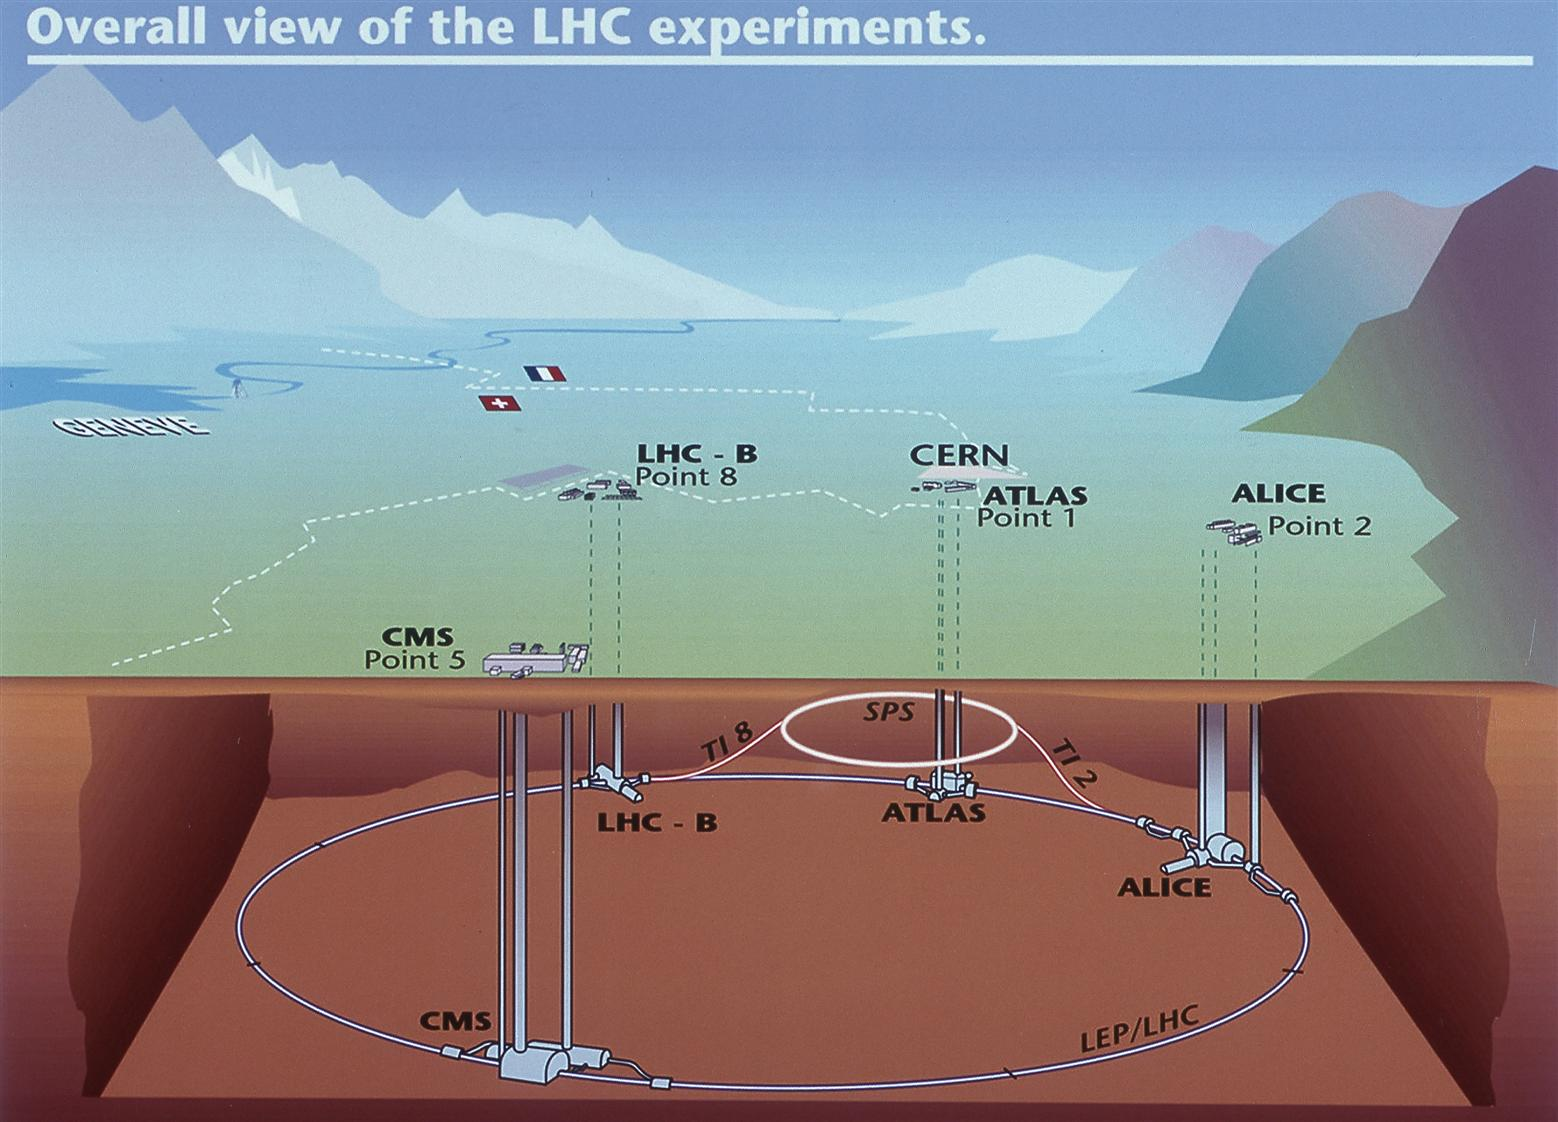
\includegraphics{figures/ch3-experiment/LHC_IPs}}
	\caption{The LHC and the four interaction points where the beams are brought into collision. The ATLAS experiment is located at interaction point 1.}
	\label{fig:LHC-IPs}
\end{figure}


The LHC project was approved in 1994 by the CERN Council, and construction proceeded over the ensuing 14 years. The collider detectors were constructed in parallel, beginning with the excavation of two additional caverns at IP1 and IP5 for the ATLAS and CMS detectors (LHCb and ALICE occupied the existing caverns at IP2 and IP8, which previously housed the DELPHI and L3 LEP experiments). The first beam was circulated on 10 September 2008; however, on 19 September, the LHC sustained severe damage due to an incident stemming from a faulty joint between magnets\footnote{A postmortem analysis implicated a bad splice between the superconducting cables of adjacent magnets as the source of the incident, with a resistance about $10^3$ times above specification. The joint melted, and 275~MJ of energy in the magnets dissipated in electric arcs, which vaporized beam pipes and breached the cryogenic vessel containing the magnets. A large amount of liquid helium entered the vacuum vessel and heated rapidly, breaking several vacuum barriers of the cryostats with a force of up to 56 tons. Ultimately, 30 dipoles and 7 quadrupoles were damaged beyond repair, and another 9 dipoles and 7 quadrupoles required repairs; 9 magnet interconnections were destroyed; 26 magnets were pushed down the tunnel; 276~MJ of energy were dissipated in electrical faults and arcs; 6 tons of helium were lost; and 2.8~km of both beam pipes were contaminated with fragments of insulation, with 1~km also contaminated with soot from molten copper and insulation.~\cite{Rossi:2010el}}. Repairs took an extra year, and the energy of the beams was reduced to $3.5-4~\mbox{TeV}$ for the first data-taking run, to mitigate the risk of another possible faulty joint. 

Proton-proton collisions at a center-of-mass energy of $\sqrt{s}=7~\mbox{TeV}$ commenced in early 2010. The LHC delivered an integrated luminosity of $\int L dt=48.1~\mbox{pb}^{-1}$ to the ATLAS detector in 2010, and $\int L dt=5.46~\mbox{fb}^{-1}$ in 2011. In 2012, the collision energy was increased to $\sqrt{s}=8~\mbox{TeV}$, and a dataset of $\int L dt=22.8~\mbox{fb}^{-1}$ was delivered. 

\subsection{The Accelerator Complex}
\begin{figure}[htbp]
	\centering
	\resizebox{3.5in}{!}{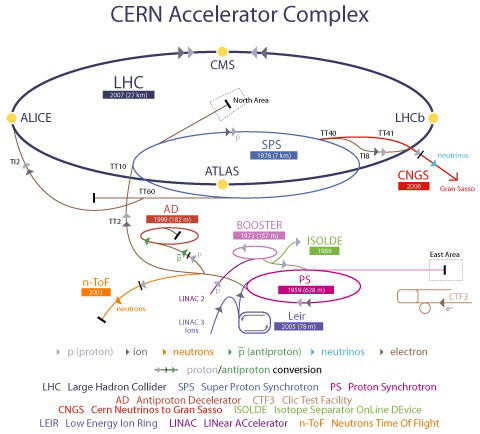
\includegraphics{figures/ch3-experiment/converted/LHC_accelerator_complex.png}}
	\caption{The LHC accelerator complex. The proton injection chain begins at LINAC2, proceeding through the booster, PS, and SPS before reaching the LHC. The facility also provides ions to the LHC, as well as a variety of particles to other experiments.}
	\label{fig:LHC-accelerator-complex}
\end{figure}


The LHC itself is the last stage of a 4-part acceleration chain, shown in figure~\ref{fig:LHC-accelerator-complex}. A full description can be found at~\cite{Benedikt:2004wm}. The staged acceleration chain meets the stringent performance requirements of the LHC, namely providing up to 2808 proton bunches with a very small transverse emittance and controllable longitudinal emittance. 

The primary devices making up the accelerators are radio frequency (RF) cavities and magnets. RF cavities are metallic structures used for particle acceleration. An example of an LHC RF cavity is shown in figure~\ref{fig:rf-cavity}. The RF cavities are driven by a power source, typically a klystron, at their resonant frequency, creating an oscillating electromagnetic field inside the structure. Proton bunches synchronized with the oscillation of the electic fields are accelerated down the cavity. 
% Talk about the bunch spacing here.

A variety of types of magnet are used to manipulate the proton beams. Dipole magnets, such as that shown in figure~\ref{fig:LHC-dipole}, provide the centripetal force that bends the beams in a circle. Quadrupole and higher order magnets focus the beams.

Protons are produced from hydrogen gas using a duoplasmatron source, which strips electrons from protons in a high electric field. After passing through a $90~\mbox{kV}$ pre-injector, a radio frequency quadrupole (RFQ) focuses and accelerates the protons to $750~\mbox{kV}$. A linear accelerator (LINAC2) then accelerates the protons to $50~\mbox{MeV}$ using RF cavities. The protons then pass through an $80~\mbox{m}$-long transfer line into the the Proton Synchrotron Booster (PSB) and Proton Synchrotron (PS). 

The PSB consists of four stacked circular synchrotrons, $157~\mbox{m}$ in circumference, and accelerates the protons to $1.4 \GeV$. The use of four separate rings mitigates the space charge effects caused by the repulsion of protons within a bunch, which scale as $N_b/(\beta\gamma^2)$, where $N_b$ is the number of protons per bunch. The protons are then injected into single-ring PS, where the higher injection energy reduces the space charge effect. The PS accelerates the beams to $25 \GeV$, and also bunches the protons in preparation for injection into the LHC. A third synchrotron in the chain, the $7~\mbox{km}$-circumference Super Proton Synchrotron (SPS), accelerates the protons to $450 \GeV$, where they are injected into the LHC. 

The protons reach a momentum of $1.4~\mbox{GeV}/c$ in the Proton Synchrotron Booster (PSB), $25~\mbox{GeV}/c$ in the Proton Synchrotron (PS), and $450~\mbox{GeV}/c$ in the Super Proton Synchrotron (SPS), before being injected into the LHC for acceleration up to the final collision energy. 


\subsection{Accelerator Parameters}
From the experiments' point of view, there are two main parameters to optimize in order to maximize sensitivity to new physics: the collision energy, $\sqrt{s}$, and the integrated luminosity, $\int L dt$. The collision energy is limited to $\sqrt{s}=14~\mbox{TeV}$ by the bending power of the dipole magnets, which have a field strength of $8.73~\mbox{T}$; however, due to the faulty splice design mentioned above, the energy was limited to $\sqrt{s}=7-8~\mbox{TeV}$ in Run I. 

The optimization of luminosity is somewhat more complicated.  The luminosity of the colliding beams is given by:
\begin{equation}\label{eqn:lumi}
	L = \frac{n_b f_r N_1 N_2 \gamma_b}{4\pi \varepsilon_n \beta_{*}},
\end{equation}
where $n_b$ is the number of colliding bunch pairs, $f_r=11245.5~\mbox{Hz}$ is the LHC revolution frequency, $N_{1,2}$ are the number of proton in the two beams, $\gamma_b$ is the relativistic gamma factor, $\varepsilon_n$ is the normalized emittance, and $\beta_{*}$ is the beta function at the collision point. TALK ABOUT THE LIMITS ON THESE NUMBERS.

In general, a higher integrated luminosity is desired; however, a high number of simultaneous collisions, $\mu=L/n_b$, can degrade the performance of the detectors. 

%\subsection{Interaction Regions}

\subsection{Run I Performance}



\section{The ATLAS Experiment}
The ATLAS detector is a large, cylindrical collider detector located at IP1 on the LHC ring (figure~\ref{fig:LHC-IPs}). The detector measures the energy and momenta of charged and colored particles produced in the collisions provided by the LHC. It consists of several subsystems occupying a cylinder , weighing (x tons). Closest to the interaction region, the inner detector performs momenta measurements of charged particles by tracking their movement through a solenoidal magnetic field (section~\ref{sec:inner-detector}). Past the inner detector solenoid magnet, electromagnetic and hadronic calorimeters measure the energy of electrons, photons, and hadrons. Finally, the muon spectrometer provides additional tracking and particle identification for muons in large toroidal magnetic field. 




\subsection{Magnets}
ATLAS relies on two powerful superconducting magnets to bend the trajectories of charged particles, allowing the tracking detectors to provide measurements of their momenta. 

% Solenoid

% Toroid


\subsection{Tracking}

\subsection{Calorimetry}

\subsection{Muon System}

\subsection{Data Acquisition}

\subsection{Data Preparation/Performance}


\printbibliography
\chapter{Dataset and Event Reconstruction}\label{ch:dataset-reconstruction}
\begin{figure}[htbp]
	\centering
	\hfill
	\subfloat[] {\label{fig:reco-luminosity-runI}
		\resizebox{0.4\textwidth}{!}{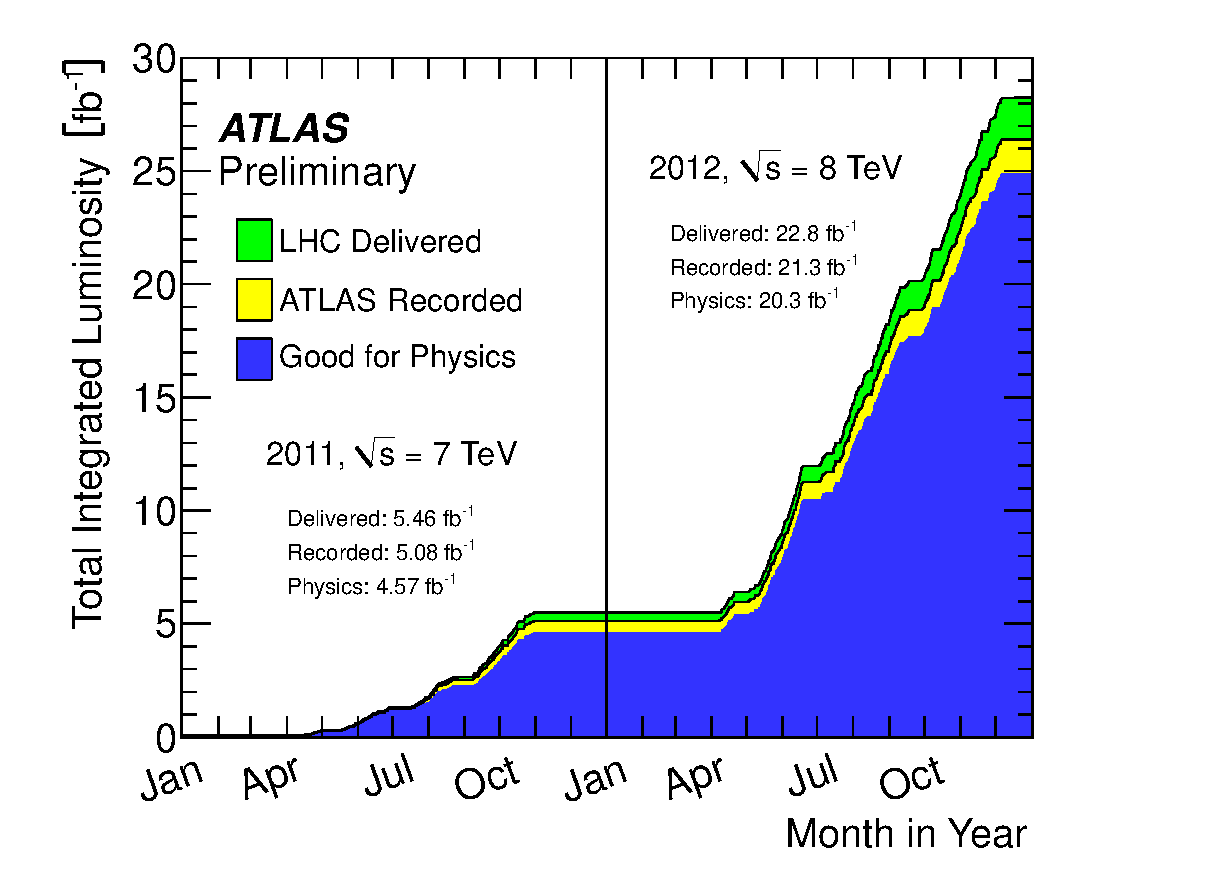
\includegraphics{figures/ch4-reconstruction/intlumivstime2011-2012DQ.eps}}
	}
	\hfill
	\subfloat[] {\label{fig:reco-luminosity-pileup}
		\resizebox{0.4\textwidth}{!}{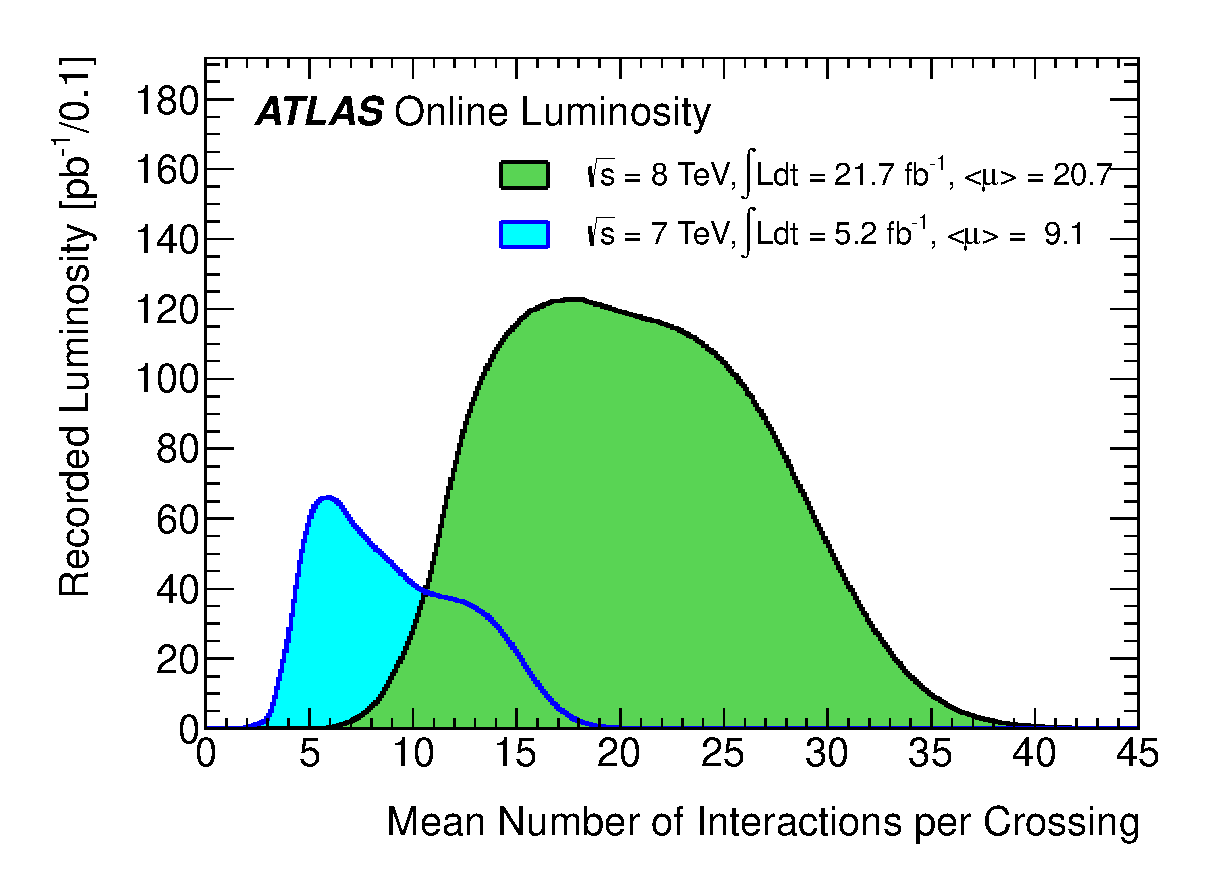
\includegraphics{figures/ch4-reconstruction/mu_2011_2012-dec.eps}}
	}
	\hfill
	\caption{Left: The cumulative delivered, recorded, and physics-ready integrated luminosity versus time in 2011-2011. Right: Distribution of the number of interactions per bunch crossing in events recorded in 2011-2012.}
	
\end{figure}

The ATLAS Run I data were recorded from 2011 to 2012, with a center-of-mass collision energy of $\sqrt{s}=7 \TeV$ in 2011 and $\sqrt{s}=8 \TeV$ during 2012. Integrated luminosities of $\int L dt=5.46 \ifb$, and $22.8 \ifb$ were delivered by the LHC in the two years, of which $5.08 \ifb$ and $21.3 \ifb$ were recorded by the ATLAS detector. The recorded luminosity accounts for the DAQ inefficiency, as well as the \emph{warm start} period after the declaration of stable beams, during which the tracking detectors are ramped to high voltage and the pixel detector preamplifiers are turned on. After masking data recorded while one or more detector subsystems were not functioning properly, $4.57 \ifb$ and $20.3 \ifb$ of data are considered ready for physics analyses. The volume of delivered, recorded, and physics-ready data are shown as a function of time in figure~\ref{fig:reco-luminosity-runI}. 

During Run I, the LHC was operated with a bunch spacing of $50 \ns$. The increases in the data-taking rate generally correspond to an increase in the number of simultaneous $pp$ interactions per bunch crossing, or \emph{pileup}, denoted $\mu$. The distribution of pileup values for 2011 and 2012 data are shown in figure~\ref{fig:reco-luminosity-pileup}. 


\section{Luminosity Measurement}\label{sec:luminosity-measurement}
The instantaneous luminosity at a $pp$ collider is given by:

\begin{equation}
	\mathcal{L} = \frac{R_{\mathrm{inel}}}{\sigma_{\mathrm{inel}}},
\end{equation}

where $R_{\mathrm{inel}}$ is the rate of inelastic $pp$ collisions, and $\sigma_{\mathrm{inel}}$ is the $pp$ inelastic cross section. For a storage ring with a revolution frequency $f_r$ and $n_b$ colliding bunch pairs, the instantaneous luminosity can be written in terms of the average number of inelastic $pp$ collisions per bunch cross, $\mu$, as 

\begin{equation}
	\mathcal{L} = \frac{\mu f_r n_b}{\sigma_{\mathrm{inel}}}.
\end{equation}

The instantaneous luminosity is measured by ATLAS using several detectors and algorithms, which have some efficiency $\epsilon$ to detect a $pp$ interaction, and measure the \emph{visible} number of interactions per bunch crossing, $\mu_{\mathrm{vis}} = \epsilon \mu$. Defining the visible cross section to be $\sigma_{\mathrm{vis}}\equiv \epsilon \sigma_{\mathrm{vis}}$, the instantaneous luminosity as measured by a particular detector is:

\begin{equation}\label{eqn:reco-luminosity-detected}
	\mathcal{L} = \frac{\mu_{\mathrm{vis}} f_r n_b}{\sigma_{\mathrm{vis}}}.
\end{equation}

The visible cross section is a calibration constant for a particular detector, which is determined during dedicated calibration runs in which the luminosity is determined directly from the geometry of the beams. The calibration procedure is described in section~\ref{sec:reco-luminosity-calibration}. 

\subsection{Luminosity Detectors}\label{sec:reco-luminosity-detectors}
ATLAS performs many redundant luminosity measurements using several detectors. The detectors fall into two categories. \emph{Event counting} detectors have a binary response, returning a 0 or 1 depending on whether a bunch crossing satisfies a set of criteria defined to detect an inelastic $pp$ collision. Such detectors essentially measure $p(0;\,\mu)$, the probability that an event falls in the first bin of a Poisson distribution, from which the mean $\mu$ be calculated. \emph{Hit counting} detectors, on the other hand, count some quantity proportional to the number of interactions in a given bunch crossing, such as the number of particles identified by a particular detector subsystem. A hit counting measurement typically yields more information about an event at the cost of additional systematic uncertainties.

Ideally, a luminosity detector exhibits the following features: 

\begin{itemize}
	\item The efficiency of the detector should be insensitive to pileup. The visible cross sections are typically measured at $\mu\approx \mathcal{O}(1)$, while a typical data-taking run has $10\lesssim\mu\lesssim50$; it is essential that the visible cross section be constant across this range of pileup values.
	\item The efficiency of the detector should also be constant over long timescales.
	\item The response of the detector and the readout should be very fast. As the LHC bunches are not identical, with different numbers of protons and emittances, it is useful to measure luminosity for each colliding bunch pair, as often as once every $25 \ns$. The colliding bunch pairs are labeled by the bunch crossing identification number, or BCID; consecutive BCIDs are separated by $25 \ns$. 
	\item The efficiency should be high enough to yield sufficient statistics. The data are used in increments as shorts at $20~$s, so the statistics collected over this time scale scale should be high enough that the total uncertainty is dominated by systematic effects. On the other hand, for event counting detectors, the efficiency should not be so high that the detector is saturated. The determination of the mean of a Poisson distribution from the first two bins requires that the first two bins both have adequate statistics. 
	\item The backgrounds should be low and understandable. Detectors can be sensitive to a wide range of phenomena aside from $pp$ collisions, which should not be counted as luminosity. For example, some detectors observe a phenomenon called afterglow, characterized by a small amount of activity in the BCIDs immediately following a collision and likely due to photons from nuclear de-excitations in the detector material. The background can be estimated using the observation that the level of afterglow background is proportional to the luminosity in the colliding BCIDs, and decays away with several time constants. Collisions between a beam and residual gas in the beam pipe, called beam-gas interactions, can also contribute a low level of background, and can be estimated by observing non-colliding bunches passing through the interaction region.
\end{itemize}

The central value of the luminosity measurement is determined by the \emph{beam conditions monitor} (BCM), which fulfills most of these desired criteria. The BCM consists of eight diamond-based particle detectors, four on each side of the interaction point at $|z|=184 \cm$ and $|\eta|=4.2$. The detectors are have a physical cross section of approximately $1 \cm^2$, and are arranged in a cross pattern, with two readouts corresponding to the vertical and horizontal pairs. The design goal of the BCM is to monitor backgrounds and to trigger a beam dump if beam losses towards the inner detector become too high; accordingly, the detector has a very fast readout, and can provide a bunch-by-bunch luminosity measurement with a time resolution of $\sim 0.7 \ns$. The luminosity is measured using event counting, and can be measured using any combination of the readouts. The configurations used require hits in either the vertical pair (BCMV) or the horizontal pair (BCMH), and either coincident hits on both sides of the interaction point (AND) or a single hit on either side (OR). The small size of the readouts leads to an efficiency of approximately 7\% in the OR configuration, which allows for sufficient statistics without saturating the detector. 

The LUCID detector provides a supplementary, bunch-by-bunch, event counting-based luminosity measurement using sixteen Cherenkov detectors surrounding the beampipe on each side of the interaction point at $|z|=17~\mbox{m}$, covering a pseudorapidity range of $5.6<|\eta|<6.0$. The Cherenkov detectors are polished aluminum tubes filled with C$_4$F$_{10}$ gas. The Cherekov photons induced by charged particles traversing the gas are collected by photomultiplier tubes (PMTs) located at the far end of the tubes. Additional Cherenkov photons are produced in the quartz window separating the tube volume from the PMT. In this initial configuration, the typical single-particle yield is 60-70 photoelectrons due to photons created in the gas, and about 40 photoelectrons due to the quartz window. A hit is recorded if the PMT signal exceeds a preset threshold, corresponding to about 15 photoelectrons. However, the higher per-bunch instantaneous luminosities due to the LHC operating with $50 \ns$ spacing rather than the design $25 \ns$ spacing led to saturation of the detectors, and hence on 30 July 2011, the gas was removed from the Cherenkov tubes to reduce the efficiency. The removal of the gas also improved the detector's stability and linearity with respect to pileup. Relative comparisons with other detectors were used to reestablish the detector calibration.

Several detector subsystems nominally designed for physics object reconstruction are also used for hit counting-based luminosity measurements. Algorithms using the tile calorimeter and the forward calorimeters (see section~\ref{sec:ATLAS-calorimeters}) determine the luminosity from detector currents proportional to the total particle flux in small regions of the calorimeters. The tile calorimeter algorithm monitors the PMT currents corresponding to a few selected cells near $|\eta|=1.25$, where the highest sensitivity to changes in the luminosity is observed. Similarly, the forward calorimeter algorithm monitors the currents in the high voltage lines. In both cases, the detector response is too slow to provide a bunch-by-bunch measurement, and the current response is not sensitive to the low instantaneous luminosities during the dedicated calibration runs, requiring the calibration to be set using a relative comparison with LUCID. On the other hand, the detectors exhibit good linearity of response with pileup, and good short-term stability. 

Finally, algorithms using the inner detector measure the luminosity by counting reconstructed vertices\footnote{Pixel cluster counting, used by the CMS experiment, was also considered, but was not commissioned due to the difficulty of the background subtraction.}. The vertex counting algorithm is expected to have good long-term stability and very low backgrounds. A primary drawback is that the data must be read out through the standard ATLAS data acquisition system, and hence the rate is limited to a few hundred Hz, sufficient only for a bunch-integrated measurement performed over several luminosity blocks. Further, the efficiency drops significantly with pileup, up to $\sim30\%$ at pileup values of $\mu=30$. Therefore, the vertex counting algorithm is useful primarily for luminosity measurements during runs with low pileup. 


\subsection{Luminosity Calibration: van der Meer Scans}\label{sec:reco-luminosity-calibration}
The visible cross sections for the detectors and algorithms described in section~\ref{sec:reco-luminosity-detectors} are calibrated during dedicated runs known as van der Meer (vdM) scans. The calibration procedure uses the definition of luminosity in terms of the beam parameters, given for a single colliding bunch by:

\begin{equation}\label{eqn:luminosity-geometrical}
	\mathcal{L} = f_r n_1 n_2 K \int \rho_1(x,y,z,t) \rho_2(x,y,z,t) dx\,dy\,dz\,dt,
\end{equation}

where $f_r$ is the revolution frequency, $n_{1,2}$ are the number of particles in the colliding bunches, and $\rho_{1,2}(x,y,z,t)$ are the time- and position-dependent particle density distribution, normalized so that $\int \rho_{1,2}(x,y,z,t)dx\,dy\,dz = 1$. $K$ is a kinematic factor,

\begin{equation}
	K=\sqrt{(\vec{v}_1-\vec{v}_2)^2 - \frac{(\vec{v}_1\times\vec{v}_2)^2}{c^2}},
\end{equation}

which, in the limit $|\vec{v}_{1,2}|\rightarrow c$, reduces to $2c\cos\alpha$, where $\alpha$ is the crossing angle between the beams. For simplicity, the crossing angle is assumed to be zero, and the bunch densities are assumed to be functions of $x$, $y$, and $z\pm ct$, i.e. that the transverse bunch profiles are constant over the duration of the collision
\footnote{Specifically, the \emph{hourglass effect} is neglected. The collisions occur in a drift space, where the beams are typically focused, or squeezed, onto the interaction point. The transverse size of the beam in direction $i$ as a function of $z$ is given by $\sigma_{i}^2(z)=\epsilon_{i} \beta^*_{i} \left(1+\frac{(z-z_{i}^w)^2}{{\beta^*_{i}}^2}\right)$, where $\epsilon_{i}$ is the transverse emittance, $z_i^w$ is location of the optical waist, and $\beta^*_i$ is the betatron function at $z=z_i^w$. The effect is significant when $\beta^*_i\lesssim \sigma_z$; during the vdM scans, $\sigma_z\approx 50 \mm$, while $\beta^*=1.5~\mbox{m}$-$11~\mbox{m}$, and hence the hourglass effect is neglected.}. The luminosity can then be expressed as:

\begin{equation}
	\mathcal{L}=f_r n_1 n_2 \int \hat{\rho}_1(x,\,y)\hat{\rho}_2(x,\,y) dx\,dy,
\end{equation}

where $\hat{\rho}_{1,2}(x,\,y)$ are the transverse particle densities, normalized to unity. Under the further assumption that the transverse particle densities factorize in the horizontal and vertical directions, $\hat{\rho}(x,\,y)=\rho_x(x)\rho_y(y)$, the luminosity can be written as:

\begin{equation}
	\mathcal{L} = f_r n_1 n_2 \Omega_x(\rho_{x1},\,\rho_{x2}) \Omega_y(\rho_{y1},\,\rho_{y2}),
\end{equation}

where $\Omega_x(\rho_{x1},\,\rho_{x2})=\int \rho_{x1}(x) \rho_{x2}(x) dx$, and similarly for the $y$ direction. As first proposed by van der Meer~\cite{vdm}, the $\Omega_{x,y}$ parameters can be determined by measuring the interaction rate $R$ as a function of transverse beam displacement $\delta$,

\begin{equation}
	\Omega_x (\rho_{x1},\,\rho_{x2}) = \frac{R_x(0)}{\int R_x(\delta) d\delta}.
\end{equation}

For convenience, define $\Sigma_{x,y}$ to be the characteristic widths of $R_{x,y}(\delta$, given by:

\begin{equation}\label{eqn:reco-luminosity-CapSigma}
	\Sigma_{x,y}=\frac{1}{\sqrt{2\pi}} \frac{\int R_{x,y}(\delta)\,d\delta}{R_{x,y}(0)}.
\end{equation}

For Gaussian beams, $\Sigma_{x,y}$ correspond to the standard deviation of $R_{x,y}(\delta)$. Finally, the luminosity is given by

\begin{equation}
	\mathcal{L} = \frac{f_r n_1 n_2}{2\pi \Sigma_x \Sigma_y}.
\end{equation}

Equating this with the luminosity defined in equation~\ref{eqn:reco-luminosity-detected}, the visible cross section for a given detector and algorithm is given by

\begin{equation}
	\sigma_{\mathrm{vis}} = \mu_{\mathrm{vis}}^{\mathrm{MAX}} \frac{2\pi \Sigma_x \Sigma_y}{n_1 n_2},
\end{equation}

where $\mu_{\mathrm{vis}}^{\mathrm{MAX}}$ is the visible interaction rate per bunch crossing at the maximum of the scan curve, $R(\delta)$. The numbers of particles per bunch, $n_{1,2}$, are measured by the LHC Bunch Current Normalization Working Group using bunch current transformers (BCTs)~\cite{BCNWG}. 

As an example, the 2011 $pp$ calibration is derived from two pairs of scans in the $x$- and $y$-directions, performed during the same LHC fill on 15 May 2011. The beams had 14 colliding bunch pairs, $\sim0.8\times 10^11$ protons per bunch, $\beta^*=1.5~\mbox{m}$, and a crossing angle of $\alpha=240~\mu\mbox{rad}$. The resulting transverse beam size is approximately $\sigma_{x}\approx\sigma_{y}\approx 40 \micron$, and the average number of interactions per cross with head-on collisions is $\mu\approx 2.3$. The scan was performed in 25 equal steps over a displacement range of $\delta=\pm 233 \micron$.

An example scan curve showing $\mu_{\mathrm{vis}}^{\mathrm{sp}}\equiv \mu_{\mathrm{vis}}/(n_1n_2)$ as a function of transverse beam separation for the BCMV\_OR algorithm is shown in figure~\ref{fig:reco-vdm-curve}. The vdM scan curve is fitted with a Gaussian plus a constant, which is used as $R_{x,y}(\delta)$ to calculate $\Sigma_{x,y}$ in equation~\ref{eqn:reco-luminosity-CapSigma}. $\mu_{\mathrm{vis}}^{\mathrm{MAX}}$ is determined from the peak of the fitted function. The measured $\sigma_{\mathrm{vis}}$ values for both scans and all 14 colliding bunch pairs are shown in figure~\ref{fig:reco-vdm-sigmavis-bcm-2011}. The luminosity-weighted mean $\sigma_{\mathrm{vis}}$ is taken as the central value, while the scatter of the 28 measurements, which is not consistent with statistical variation, is taken as a systematic uncertainty on the reproducibility of the measurement. 

The visible cross sections for several algorithms using during 2011 are shown in table~\ref{table:reco-luminosity-sigmavis-summary}, along with the efficiency assuming a total inelastic cross section of $\sigma_{\mathrm{inel}}= 71.34~\mbox{mb}$~\cite{TheATLASCollaboration:2014jo}.

\begin{table}[htbp]
	\centering
	\begin{tabular}{|l|c|c|}
		\hline
		Algorithm & $\sigma_{\mathrm{vis}}$ (2011) & $\frac{\sigma_{\mathrm{vis}}}{\sigma_{\mathrm{inel}}}$ \\
		\hline
		BCM\_VOR					&	$4.82\pm0.07$	&	$0.068$ \\
		\hline
		BCM\_HOR					&	$4.78\pm0.07$	&	$0.067$ \\
		\hline
		BCM\_VAND					&	$0.142\pm0.002$	&	$0.002$ \\
		\hline
		BCM\_HAND					&	$0.140\pm0.002$	&	$0.002$ \\
		\hline
		LUCID\_OR					&	$43.3\pm0.7$	&	$0.607$ \\
		\hline
		LUCID\_AND					&	$13.7\pm0.2$	&	$0.192$ \\
		\hline
		Vertexing ($\geq5$ tracks)	&	$39.1\pm0.6$	&	$0.548$ \\
		\hline
	\end{tabular}
	\caption{Visible cross sections for $pp$ luminosity measurement algorithms used in 2011. The efficiency of detecting a $pp$ collision is also shown for $\sigma_{\mathrm{inel}}=71.34~\mbox{mb}$.}
	\label{table:reco-luminosity-sigmavis-summary}
\end{table}


\subsection{Systematic Uncertainties}\label{sec:reco-luminosity-uncertainties}
The systematic uncertainty on the 2011 and 2012 luminosity measurements are 1.8\% and 2.8\%\footnote{Preliminary uncertainty. The final uncertainty is expected to be below 2\%.}, respectively. No single source of uncertainty dominates the total; rather, the uncertainty is due to many sources, each contributing less than $1\%$. The sources of uncertainty on the 2011 luminosity measurement are shown in table~\ref{table:reco-luminosity-uncertainties}, divided into uncertainties on the visible cross section measurement during vdM scans and uncertainties on the measurement performed over the course of data taking. 

The combined uncertainty on the visible cross sections due to the vdM calibration procedure is $1.5\%$. The largest source of uncertainty is due to emittance growth and non-reproducibility, reflected in the scatter between BCIDs and between scans in figure~\ref{fig:reco-vdm-sigmavis-bcm-2011}. Other significant sources, each roughly $0.5\%$, include beam-beam effects, where the two colliding beams deflect each other away from the nominal transverse separation; transverse correlations which violate the assumption that the transverse particle densities factorize as $\rho(x,\,y)=\rho_x(x)\rho_y(y)$; pileup dependence; and the measurement of the number of protons per bunch, $n_{1,2}$. 

Uncertainties on the luminosity measurement over the 2011 data-taking period total $0.9\%$. These uncertainties are dominated by variations in the detector calibrations during 2011, quantified using relative comparisons between algorithms across the entire year, and pileup dependence, quantified using relative comparisons between algorithms at different pileup values. The relative comparisons are shown in figure~\ref{fig:reco-luminosity-comparisons}.

\begin{table}[htbp]
	\centering
	\scriptsize
	\begin{tabular}{ccl}
		\hline
		Source & Uncertainty & \\
		\hline
		Bunch population product ($n_1n_2$) & {$0.5\%$} & \multirow{13}{*}{$\left.\begin{array}{c}\ \\ \ \\ \ \\ \ \\ \ \\ \ \\ \ \\ \ \\ \ \\ \ \\ \ \\ \ \\ \end{array}\right\}$ \begin{tabular}{c}vdM Calibration subtotal=$1.5\%$ \\ {Uncertainties from a single}\\ {measurement of $\sigma_{\textrm{vis}}$} \end{tabular}}\\
		Beam centering & $0.10\%$ & \\
		Beam position jitter & $0.30\%$ & \\
		{Emittance growth/non-reproducibility} & \multirow{2}{*}{{$\oplus$}\begin{tabular}{c}{$0.67\%$} \\ {$0.55\%$} \end{tabular}} & \\
		{Bunch-to-bunch $\sigma_{\textrm{vis}}$ consistency} &  & \\
		Fit model & $0.28\%$ & \\
		Background subtraction & $0.31\%$ & \\
		Specific luminosity & $0.29\%$ & \\
		Length scale calibration & $0.30\%$ & \\
		Absolute ID length scale & $0.30\%$ & \\
		{Beam-beam effects} & {$0.50\%$} & \\
		{Transverse correlations} & {$0.50\%$} & \\
		{Pileup dependence} & {$0.50\%$} & \\
		\hline
		Afterglow correction & $0.2\%$ & \multirow{4}{*}{$\left.\begin{array}{c}\ \\ \ \\ \ \\ \ \\ \end{array}\right\}$ \begin{tabular}{c}$\mathcal{L}$ measurement subtotal=$0.9\%$ \\ {Uncertainties evaluated from}\\{all 2011 physics runs}\end{tabular}}\\
		BCM Stability & $0.2\%$ & \\
		{Long-term consistency} & {$0.7\%$} & \\
		{Pileup dependence} & {$0.5\%$} & \\
		\hline
		\hline
		Total & 1.8\% & \\
		\hline
	\end{tabular}
\end{table}

\begin{figure}
	\centering
	\hfill
	\subfloat[] {\label{fig:reco-luminosity-comparisons-long-term-stability}
		\resizebox{0.45\textwidth}{!}{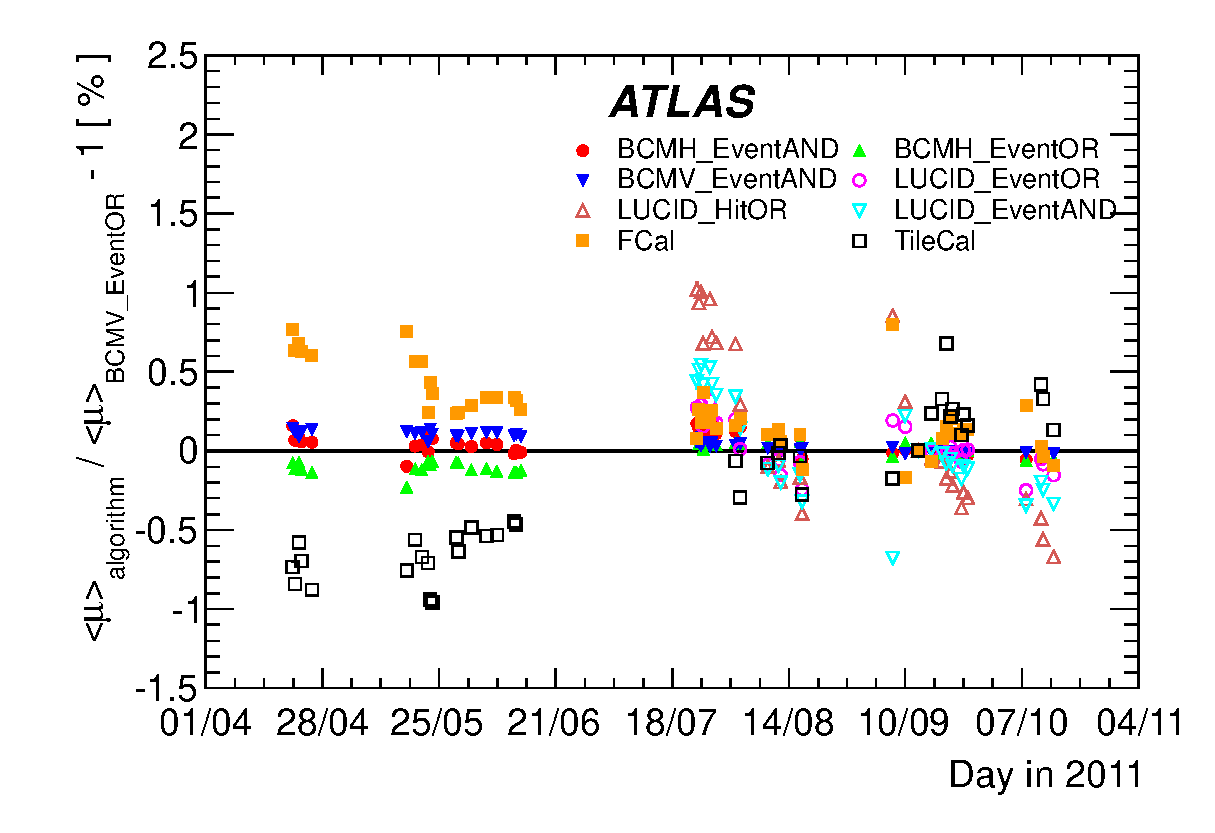
\includegraphics{figures/ch4-reconstruction/luminosity_long_term_stability}}
	}
	\hfill
	\subfloat[] {\label{fig:reco-luminosity-comparisons-pileup}
		\resizebox{0.45\textwidth}{!}{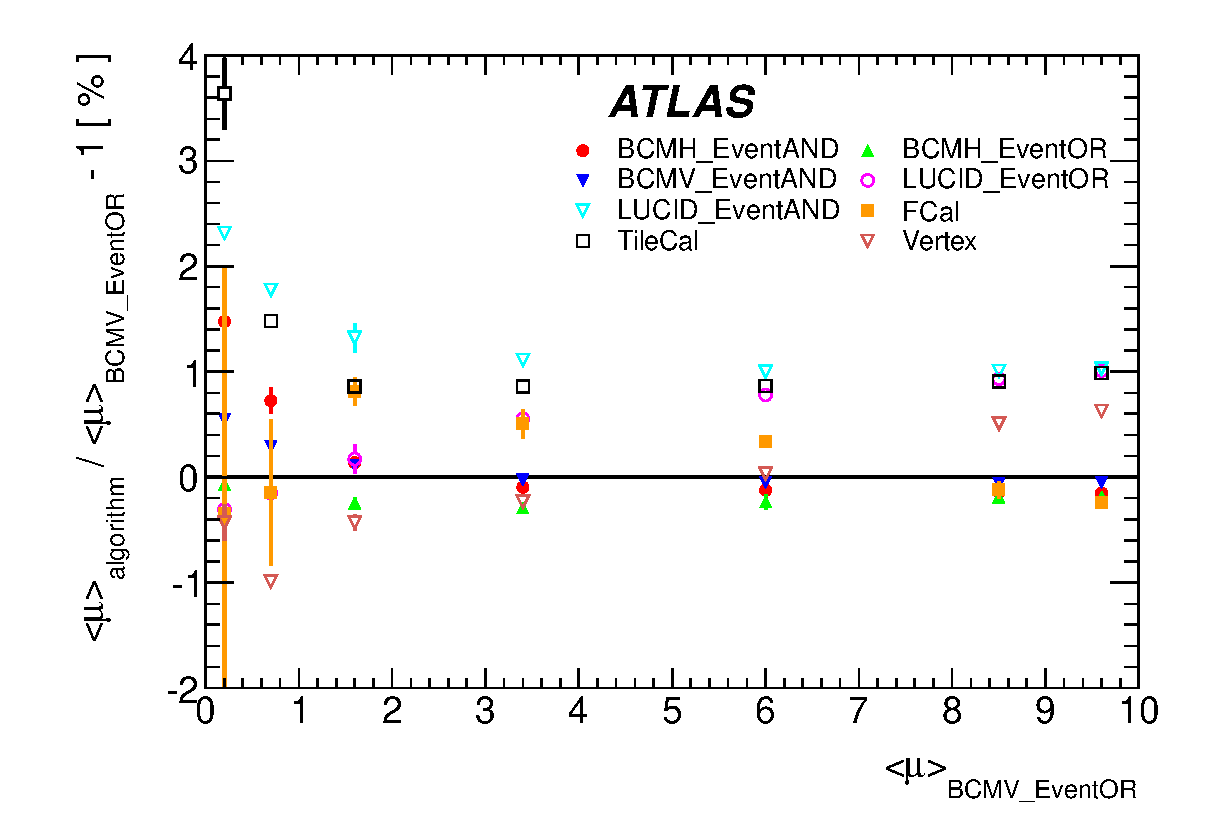
\includegraphics{figures/ch4-reconstruction/luminosity_pileup_muscan}}
	}
	\hfill
	\caption{Left:  Comparison of luminosities measured by different algorithms as a function of time in 2011. Right:  Comparison of luminosities measured by different algorithms as a function of the average number of interactions per bunch cross, $\mu$, as measured by BCM\_VOR. The data were taken during a single run by separating the beams in the transverse direction, similar to a van der Meer scan.}
	\label{fig:reco-luminosity-comparisons}
\end{figure}

\subsection{Vertex-Based Luminosity Measurement}

\subsubsection{Track and Vertex Reconstruction}

Vertices are points consistent with being the origin of a set of tracks reconstructed by the inner detector. The tracks, nominally due to charged particles traversing the inner detector, are reconstructed by a series of algorithms based on hits in inner detector~\cite{TheATLASCollaboration:2010vk}. The algorithm begins by constructing three-dimensional space points associated with the hits in the pixel and SCT layers. Track seeds are formed from sets of three space points in the first four layers of the inner detector (three pixel layers and the innermost SCT layer), constrained to be consistent with a track originating from the interaction region. The track seeds are extended through the remaining SCT layers using a combinatorial Kalman filter. After screening the track candidates to reduce random coincidences and ambiguities from very close tracks, the tracks are extended through the TRT. Finally, the track is refitted using all of the associated hits. 

The vertex reconstruction algorithm reconstructs vertices one by one, alternately finding a vertex seed and then fitting the corresponding tracks. The tracks are required to have $\pt>400 \MeV$, no missing hits where expected (\emph{holes}) in the pixel layers, and at most two holes in the SCT layers. The seed finding identifies the global maximum in the distribution of $z$ coordinates of the tracks. The vertex position is then determined by an adaptive vertex fitting algorithm~\cite{Fruhwirth:2007hz}, a $\chi^2$-based fit which suppresses the contribution from outlier tracks. In most cases, the position of the interaction region is also used as a constraint in the fit; however, for the luminosity measurement using vertices, the constraint is not applied to avoid biases due to changes in the size of the interaction region. Tracks whose impact parameter is inconsistent by more than $7\sigma$ with the vertex position are then reused to seed a new vertex, until no further seeds can be found. 

\subsubsection{Vertex Counting Method}
Vertex counting is an appealing luminosity measurement technique for a number of reasons. The backgrounds are very low, and can be controlled by requiring a minimum number of tracks per vertex, chosen to be at least five tracks in this analysis. Further, the vertex reconstruction efficiency is expected to be stable throughout the data-taking period. However, the technique has two significant drawbacks. First, the data is collected through the standard ATLAS data acquisition system, limiting the rate during normal physics runs to $\mathcal{O}(100~\mbox{Hz})$. Depending on the trigger used, a correction for the trigger deadtime may also be necessary. Second, the efficiency of the vertex reconstruction algorithm is significantly nonlinear with pileup, with the efficiency decreasing by $\sim20\%$ between pileup values of $\mu=1$ and $\mu=30$. 

The nonlinear efficiency with respect to pileup is due to three phenomena:

\begin{itemize}
	\item Vertex masking: a $pp$ interaction fails to be reconstructed as a vertex because some or all of its tracks are used by an earlier vertex in the iterative algorithm. 
	\item Fake vertices: a vertex passes the cut on the minimum number of tracks due to acquiring tracks from another nearby $pp$ interaction.
	\item Split vertices: a single interaction is reconstructed as two separate vertices.
\end{itemize}

Split vertices are a significant effect when considering all vertices with at least two tracks, but is negligible for vertices with at least five tracks. Fake vertices are a subdominant but significant effect. A correction is derived using truth matching in minimum bias Monte Carlo simulation. The simulation sample was generated using \pythia~8, with tune A2M~\cite{pythia}. For a given cut on the minimum number of tracks per vertex, $m$, a reconstructed vertex is labelled as fake if less than $m$ of its tracks are matched to charged particles originating from the same generated $pp$ interaction.

The average number of reconstructed vertices labelled as fake by Monte Carlo truth matching is shown as a function of pileup in figure~\ref{fig:fake-fractions}. The fake fractions show a significant dependence on $\mu$ and on the minimum number of tracks per vertex.

\begin{figure}[h]
	\centering
	\resizebox{5in}{!}{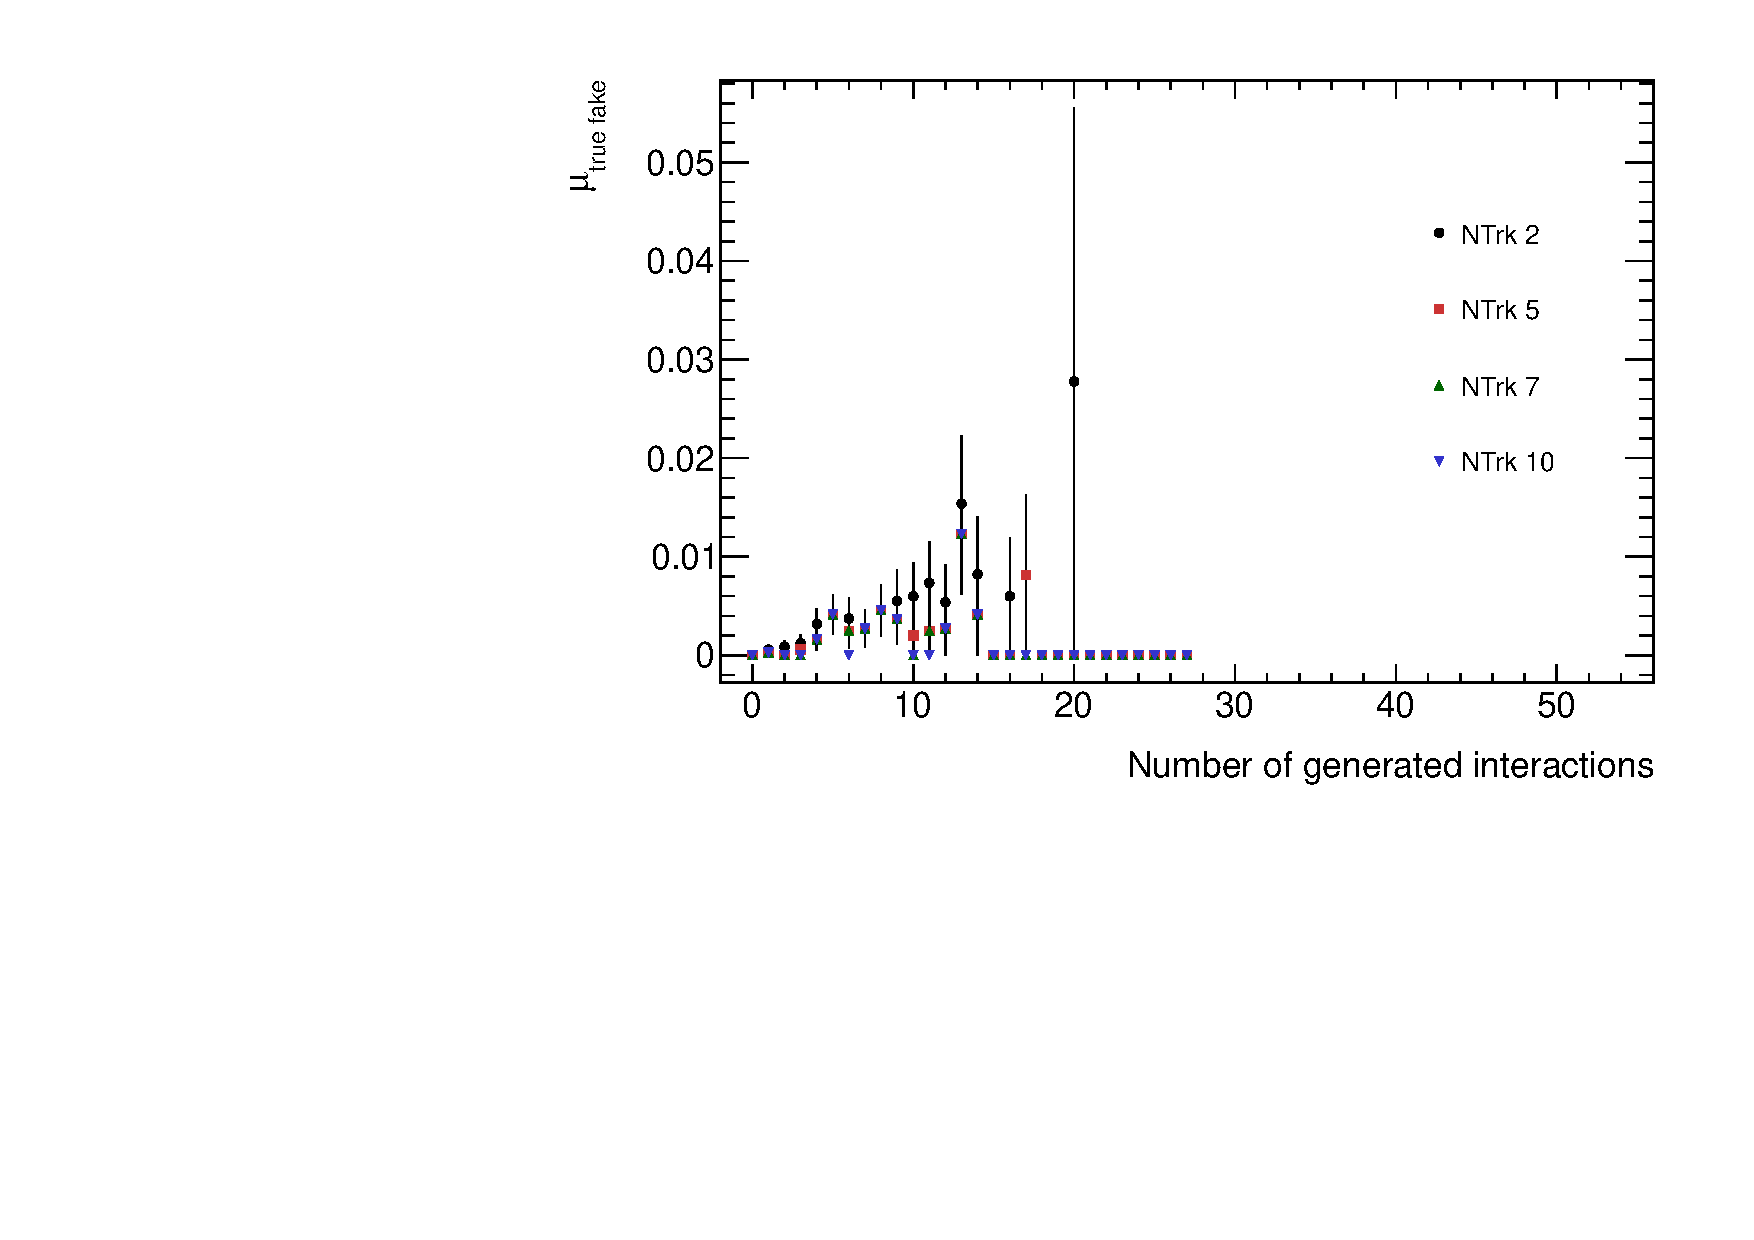
\includegraphics{figures/ch4-reconstruction/c_truefakemu_NGenInt.pdf}}
	\caption{Average number of reconstructed vertices without a matched truth interaction, as a function of number of generated interactions per event. The contribution is below 0.1\%.}
	\label{fig:truefakes}
\end{figure}

\begin{figure}[h]
	\centering
	\subfloat[$\mu_{\textrm{fake}}$ vs. number of generated interactions per event.] {
		\resizebox{3in}{!}{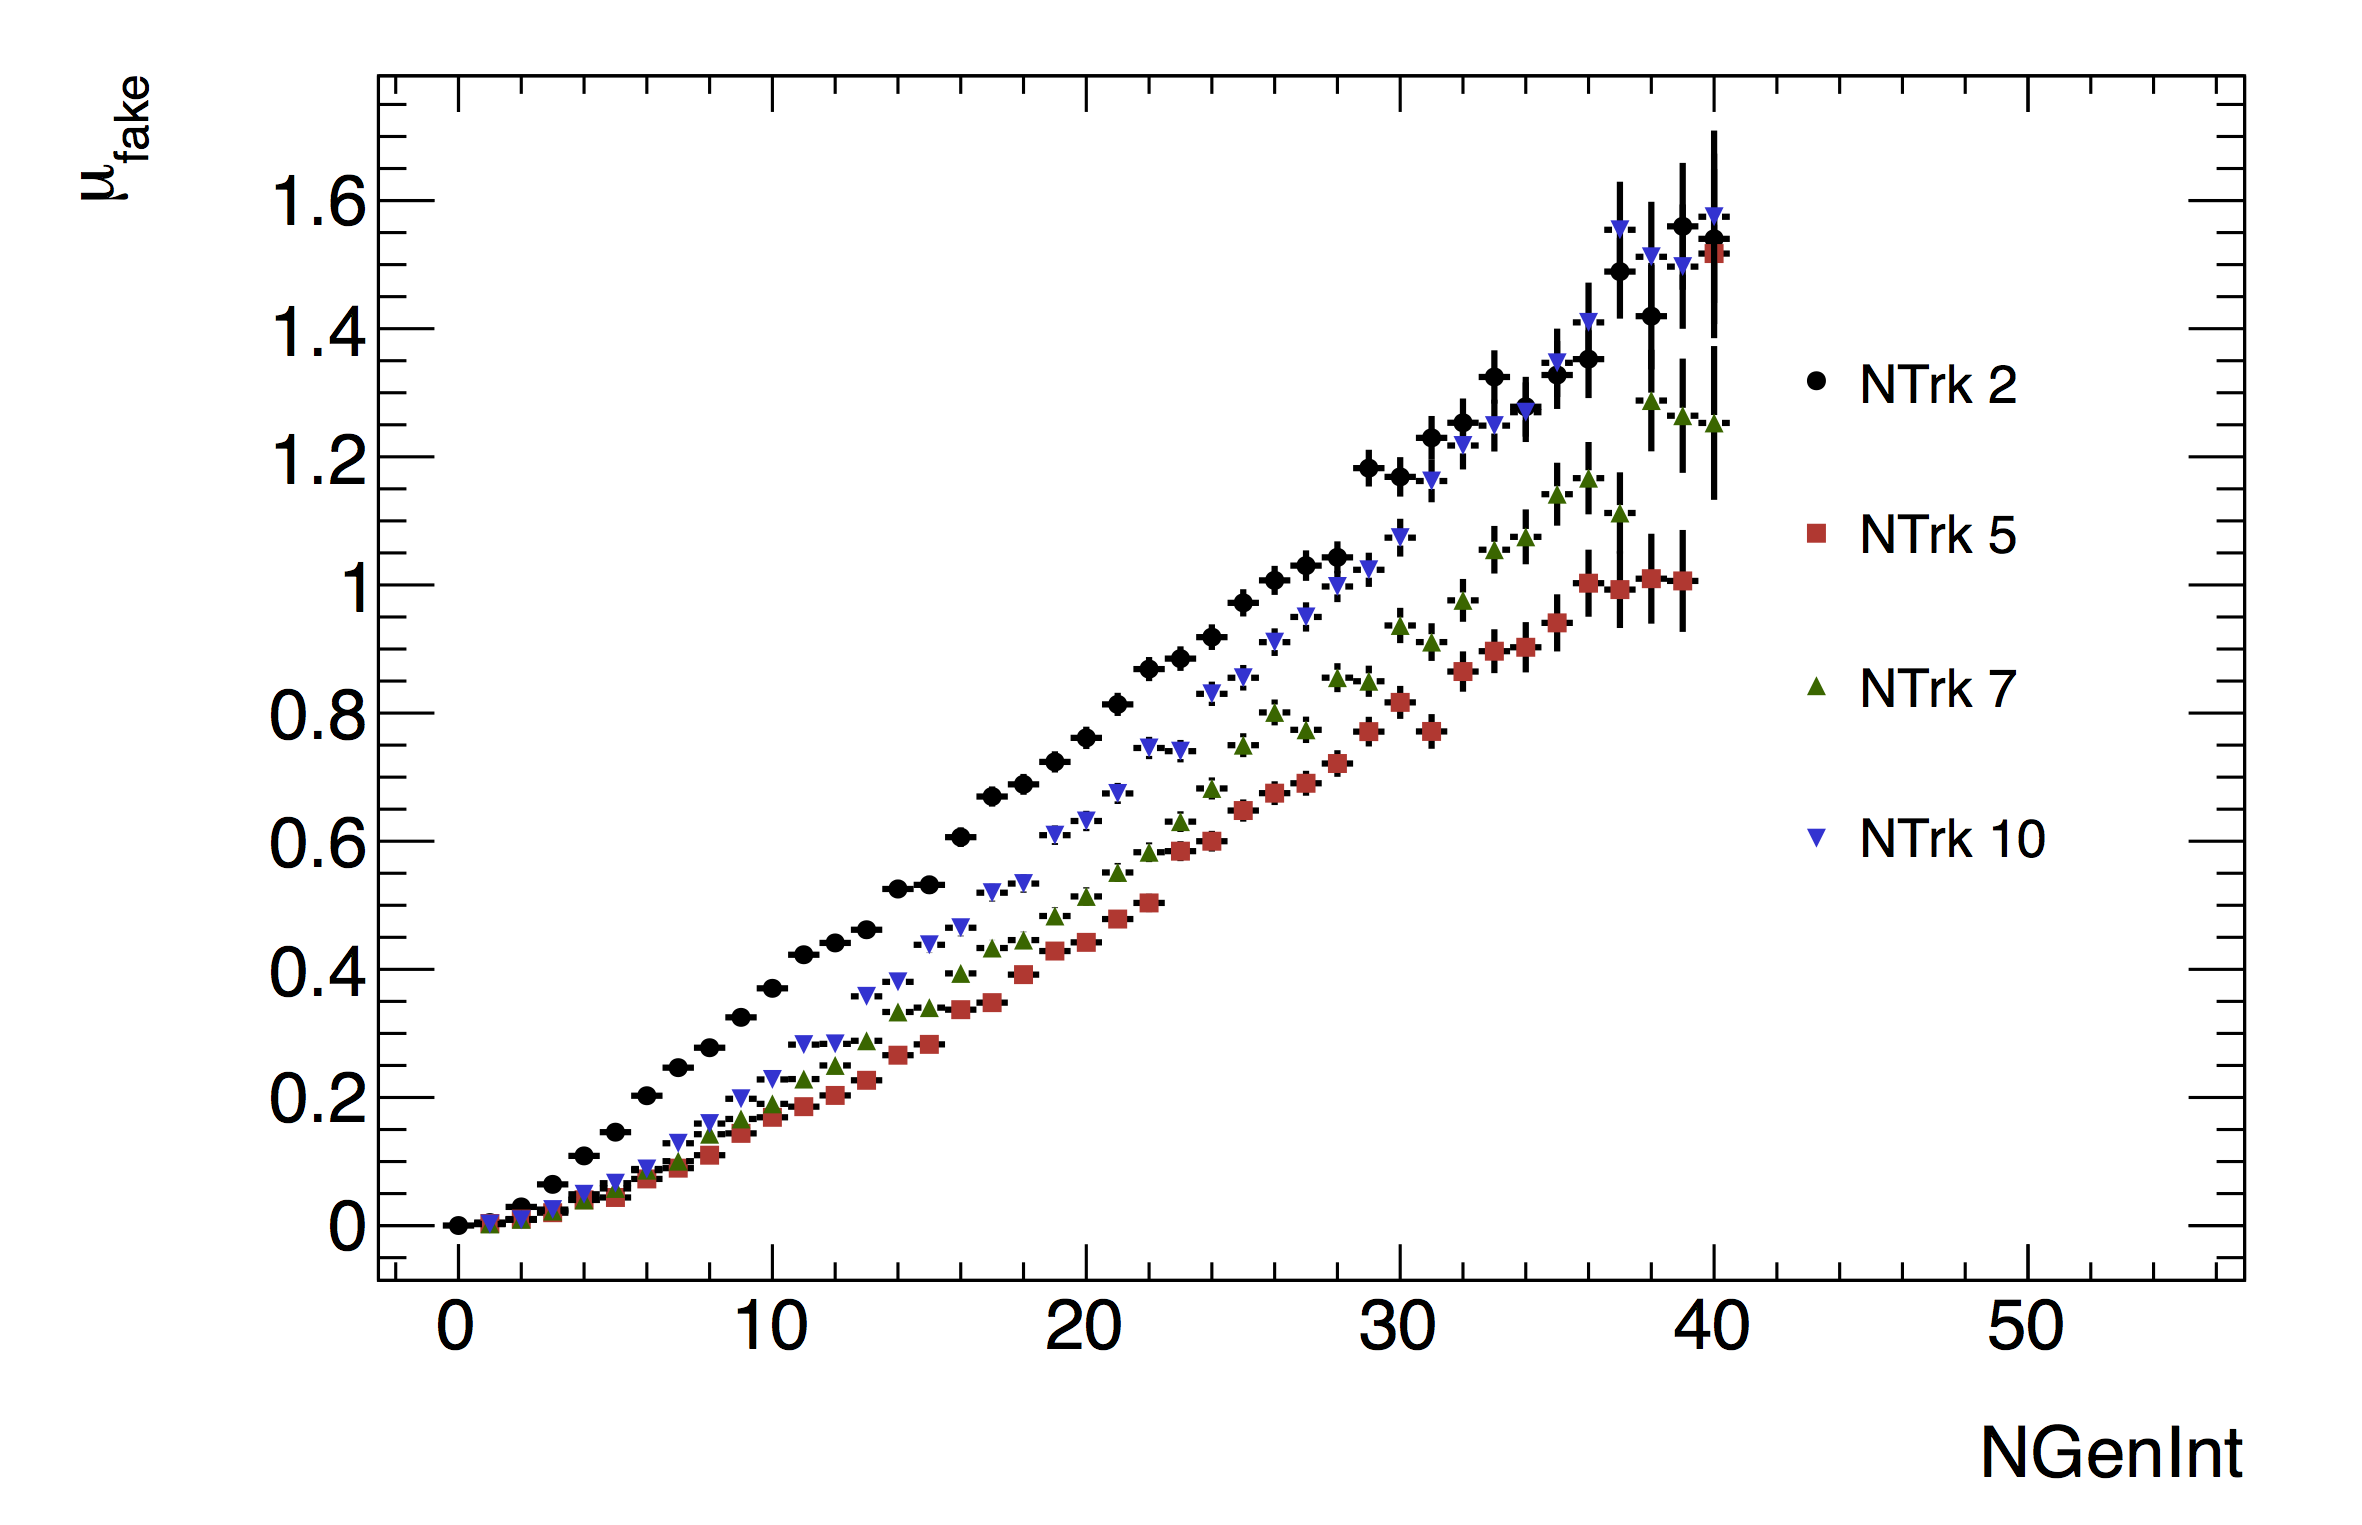
\includegraphics{figures/ch4-reconstruction/c_mu_fake_NGenInt.png}}
	}
	\subfloat[$\mu_{\textrm{fake}}$ vs. $\mu_{\textrm{inel}}$.] {
		\resizebox{3in}{!}{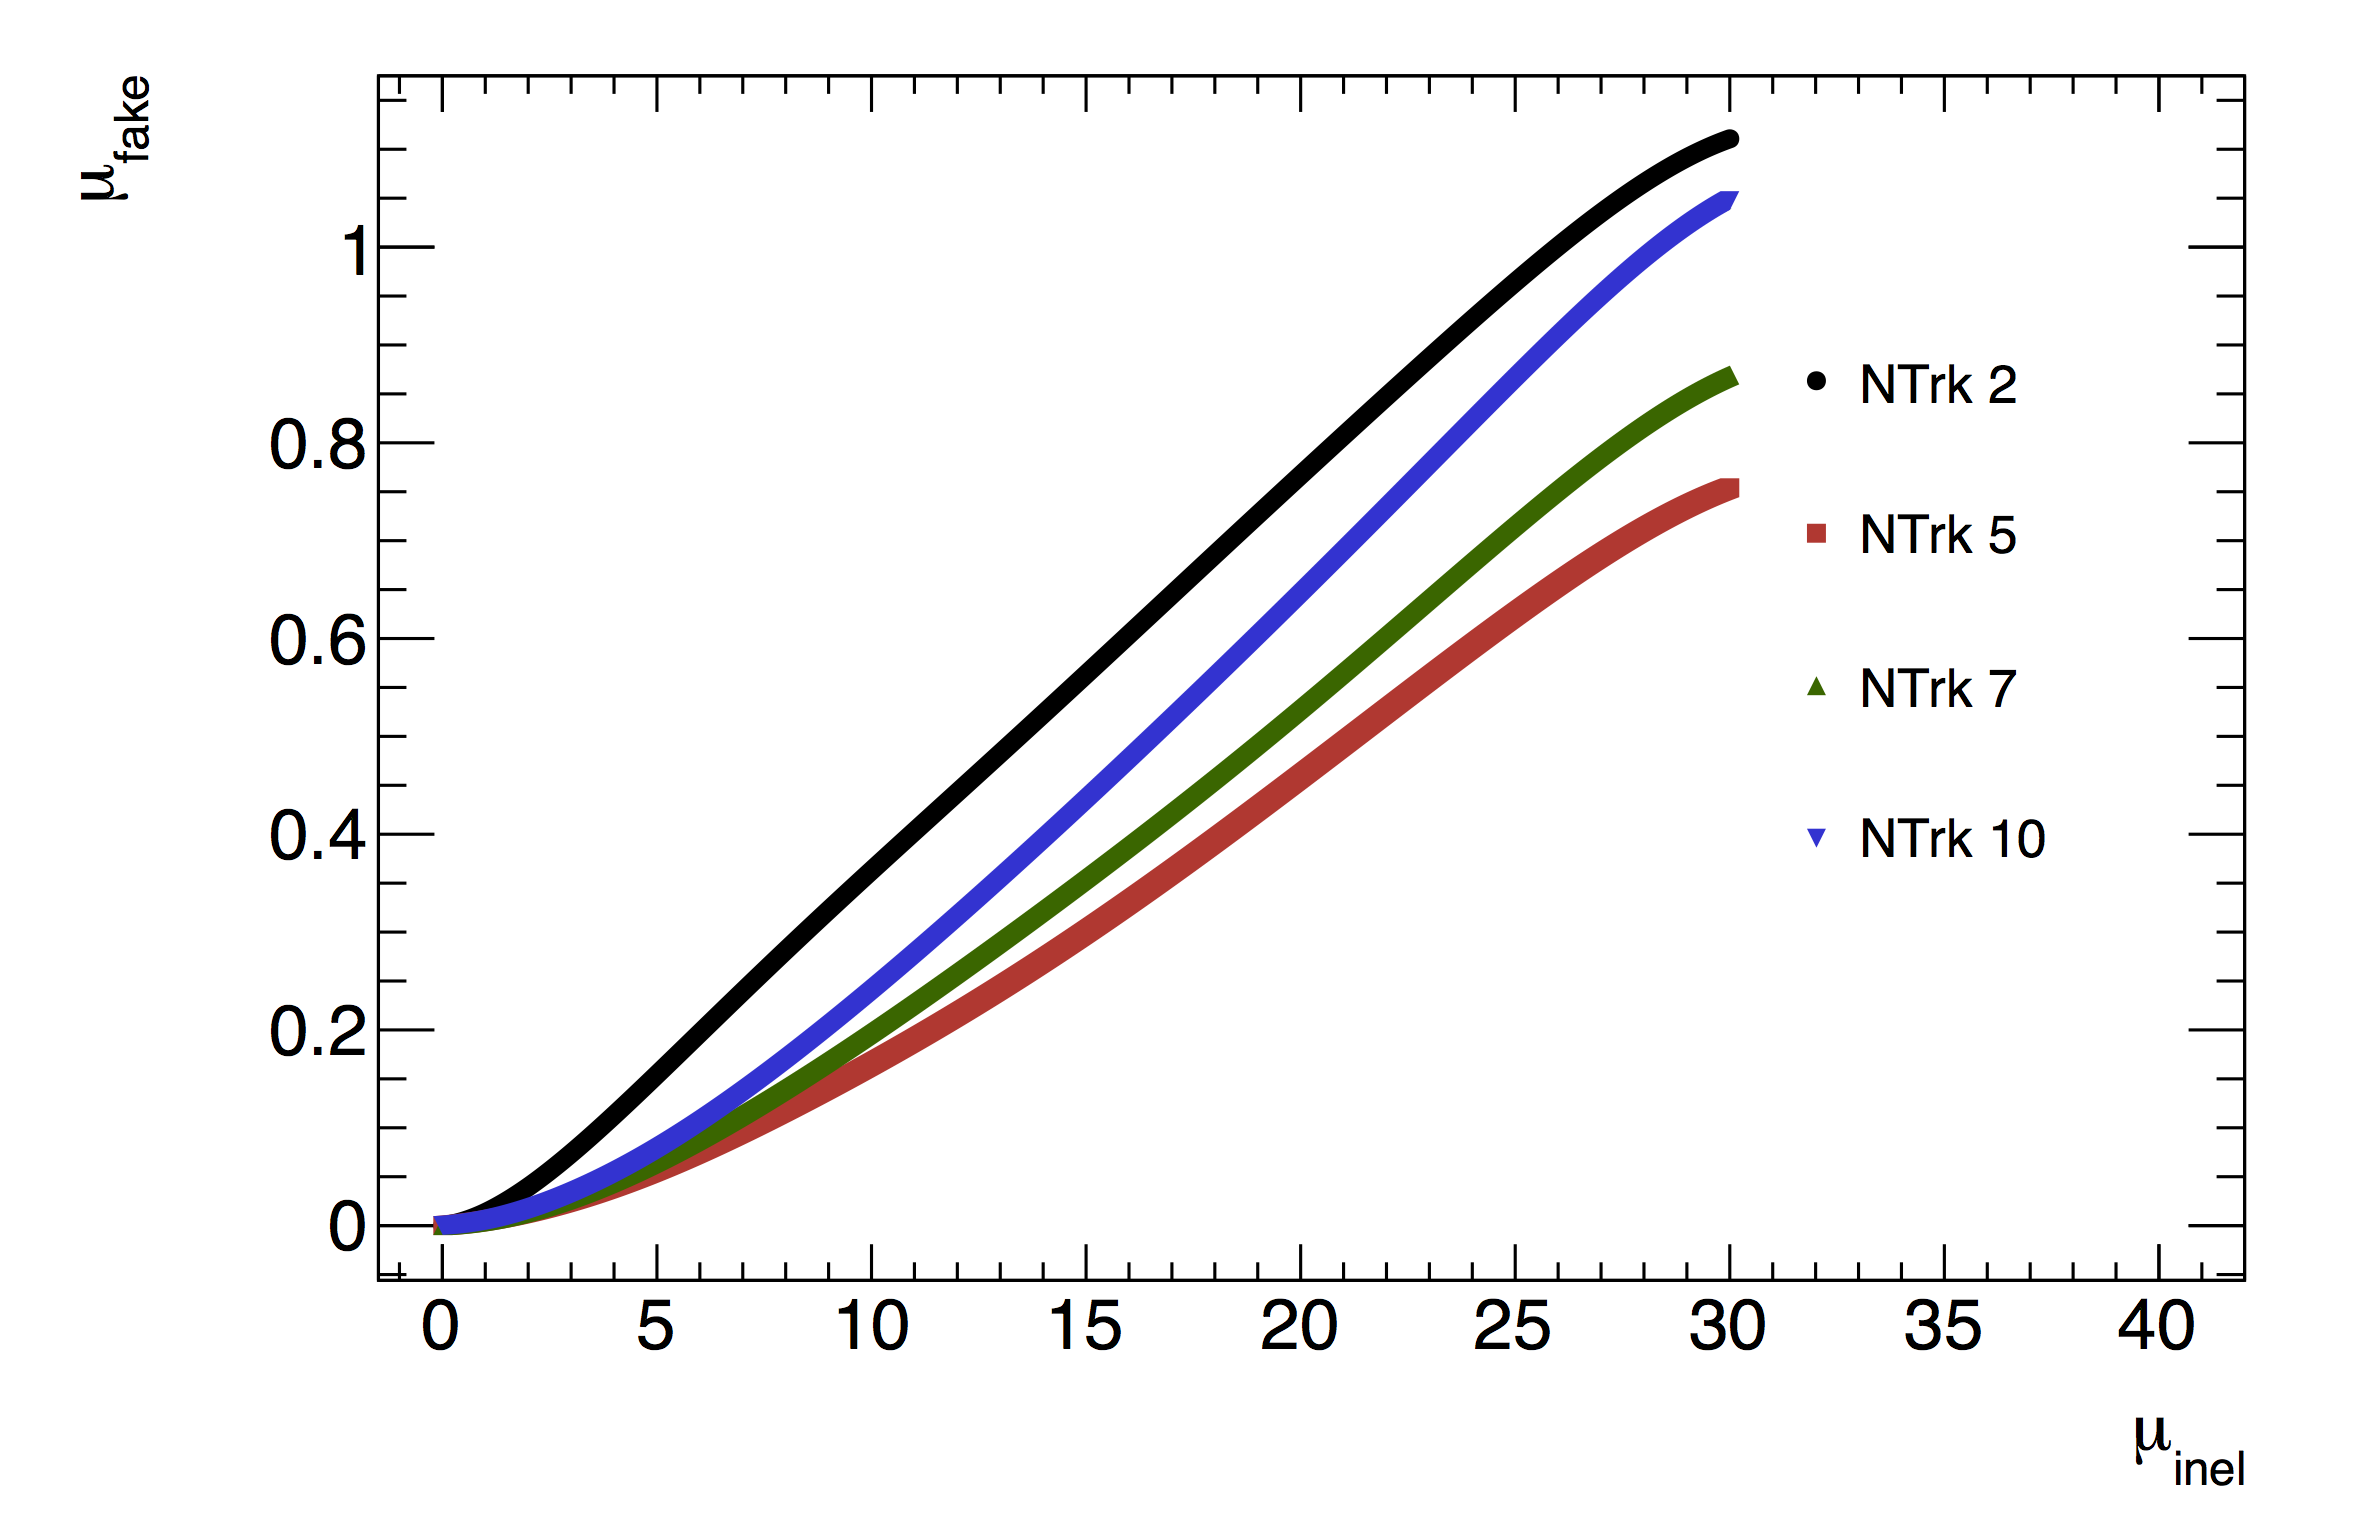
\includegraphics{figures/ch4-reconstruction/c_mu_fake_mu.png}}
	}\\
	\subfloat[$\mu_{\textrm{fake}}$ vs. $\mu_{\textrm{rec}}$ after masking correction.] {
		\resizebox{3in}{!}{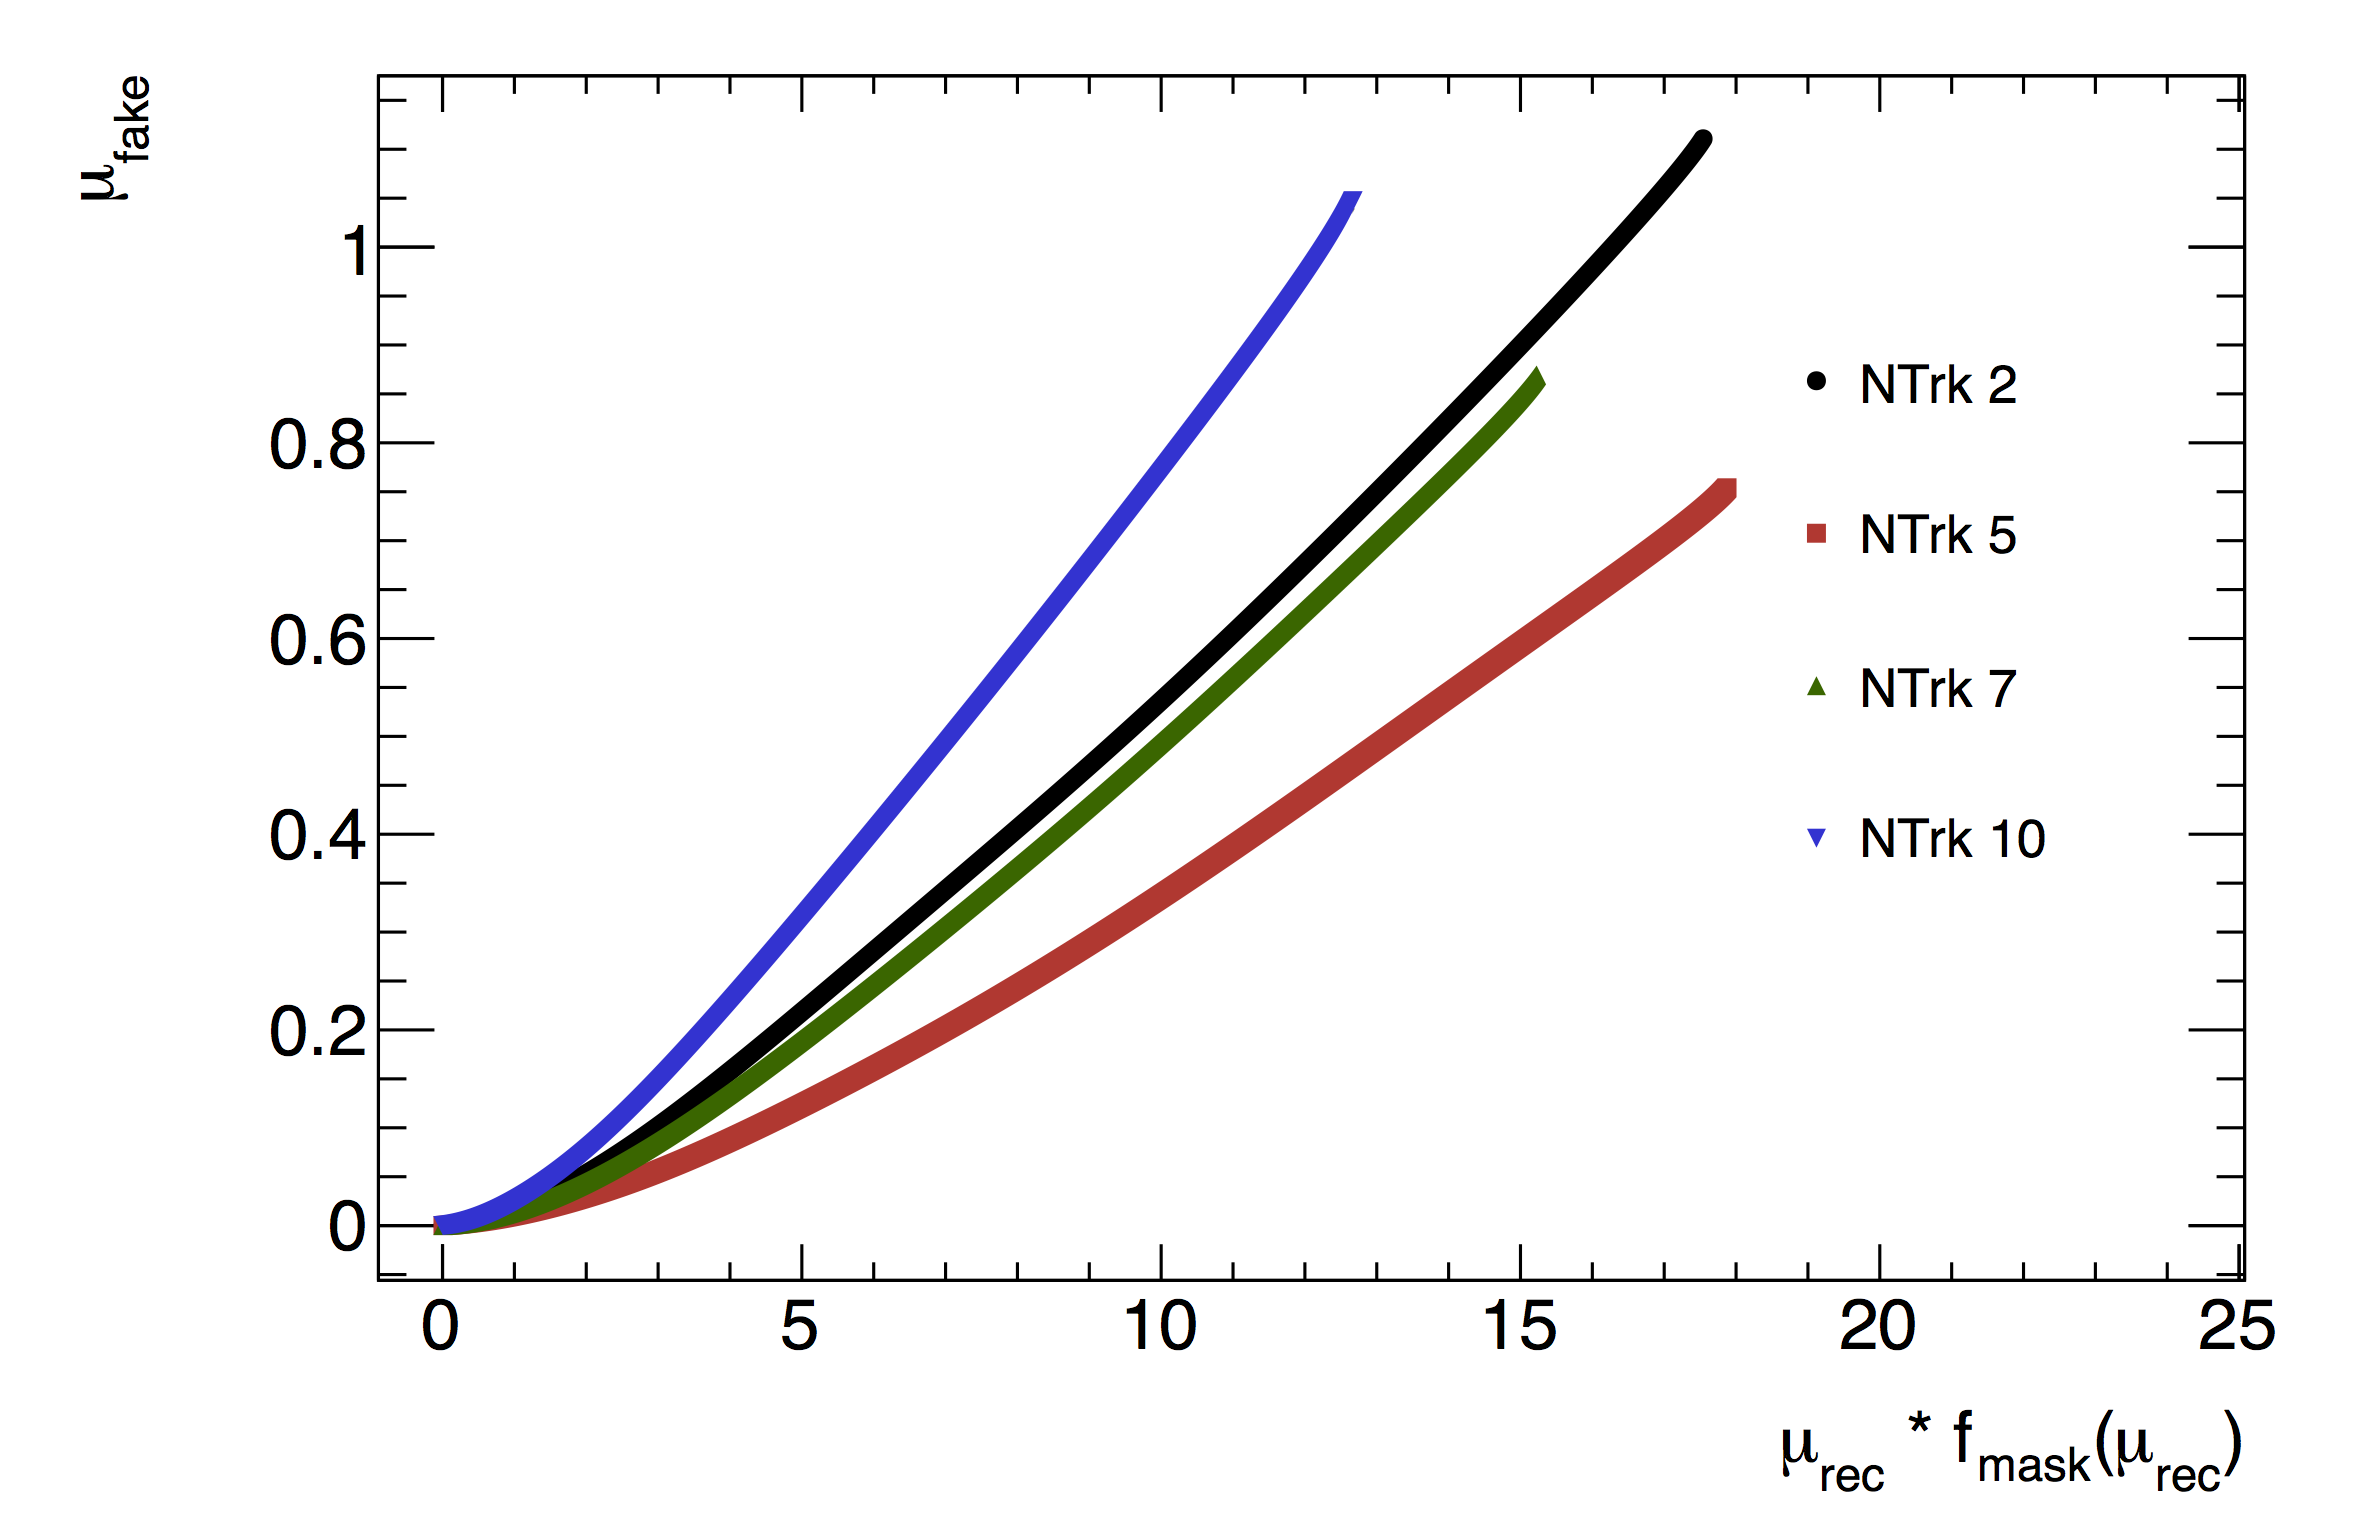
\includegraphics{figures/ch4-reconstruction/c_mu_fake_MuReconMC.png}}
		\label{fig:fake-mu-murecmc}
	}
	\subfloat[$\mu_{\textrm{fake}} / \mu_{\textrm{rec}}$ vs. $\mu_{\textrm{rec}}$ after masking correction.] {
		\resizebox{3in}{!}{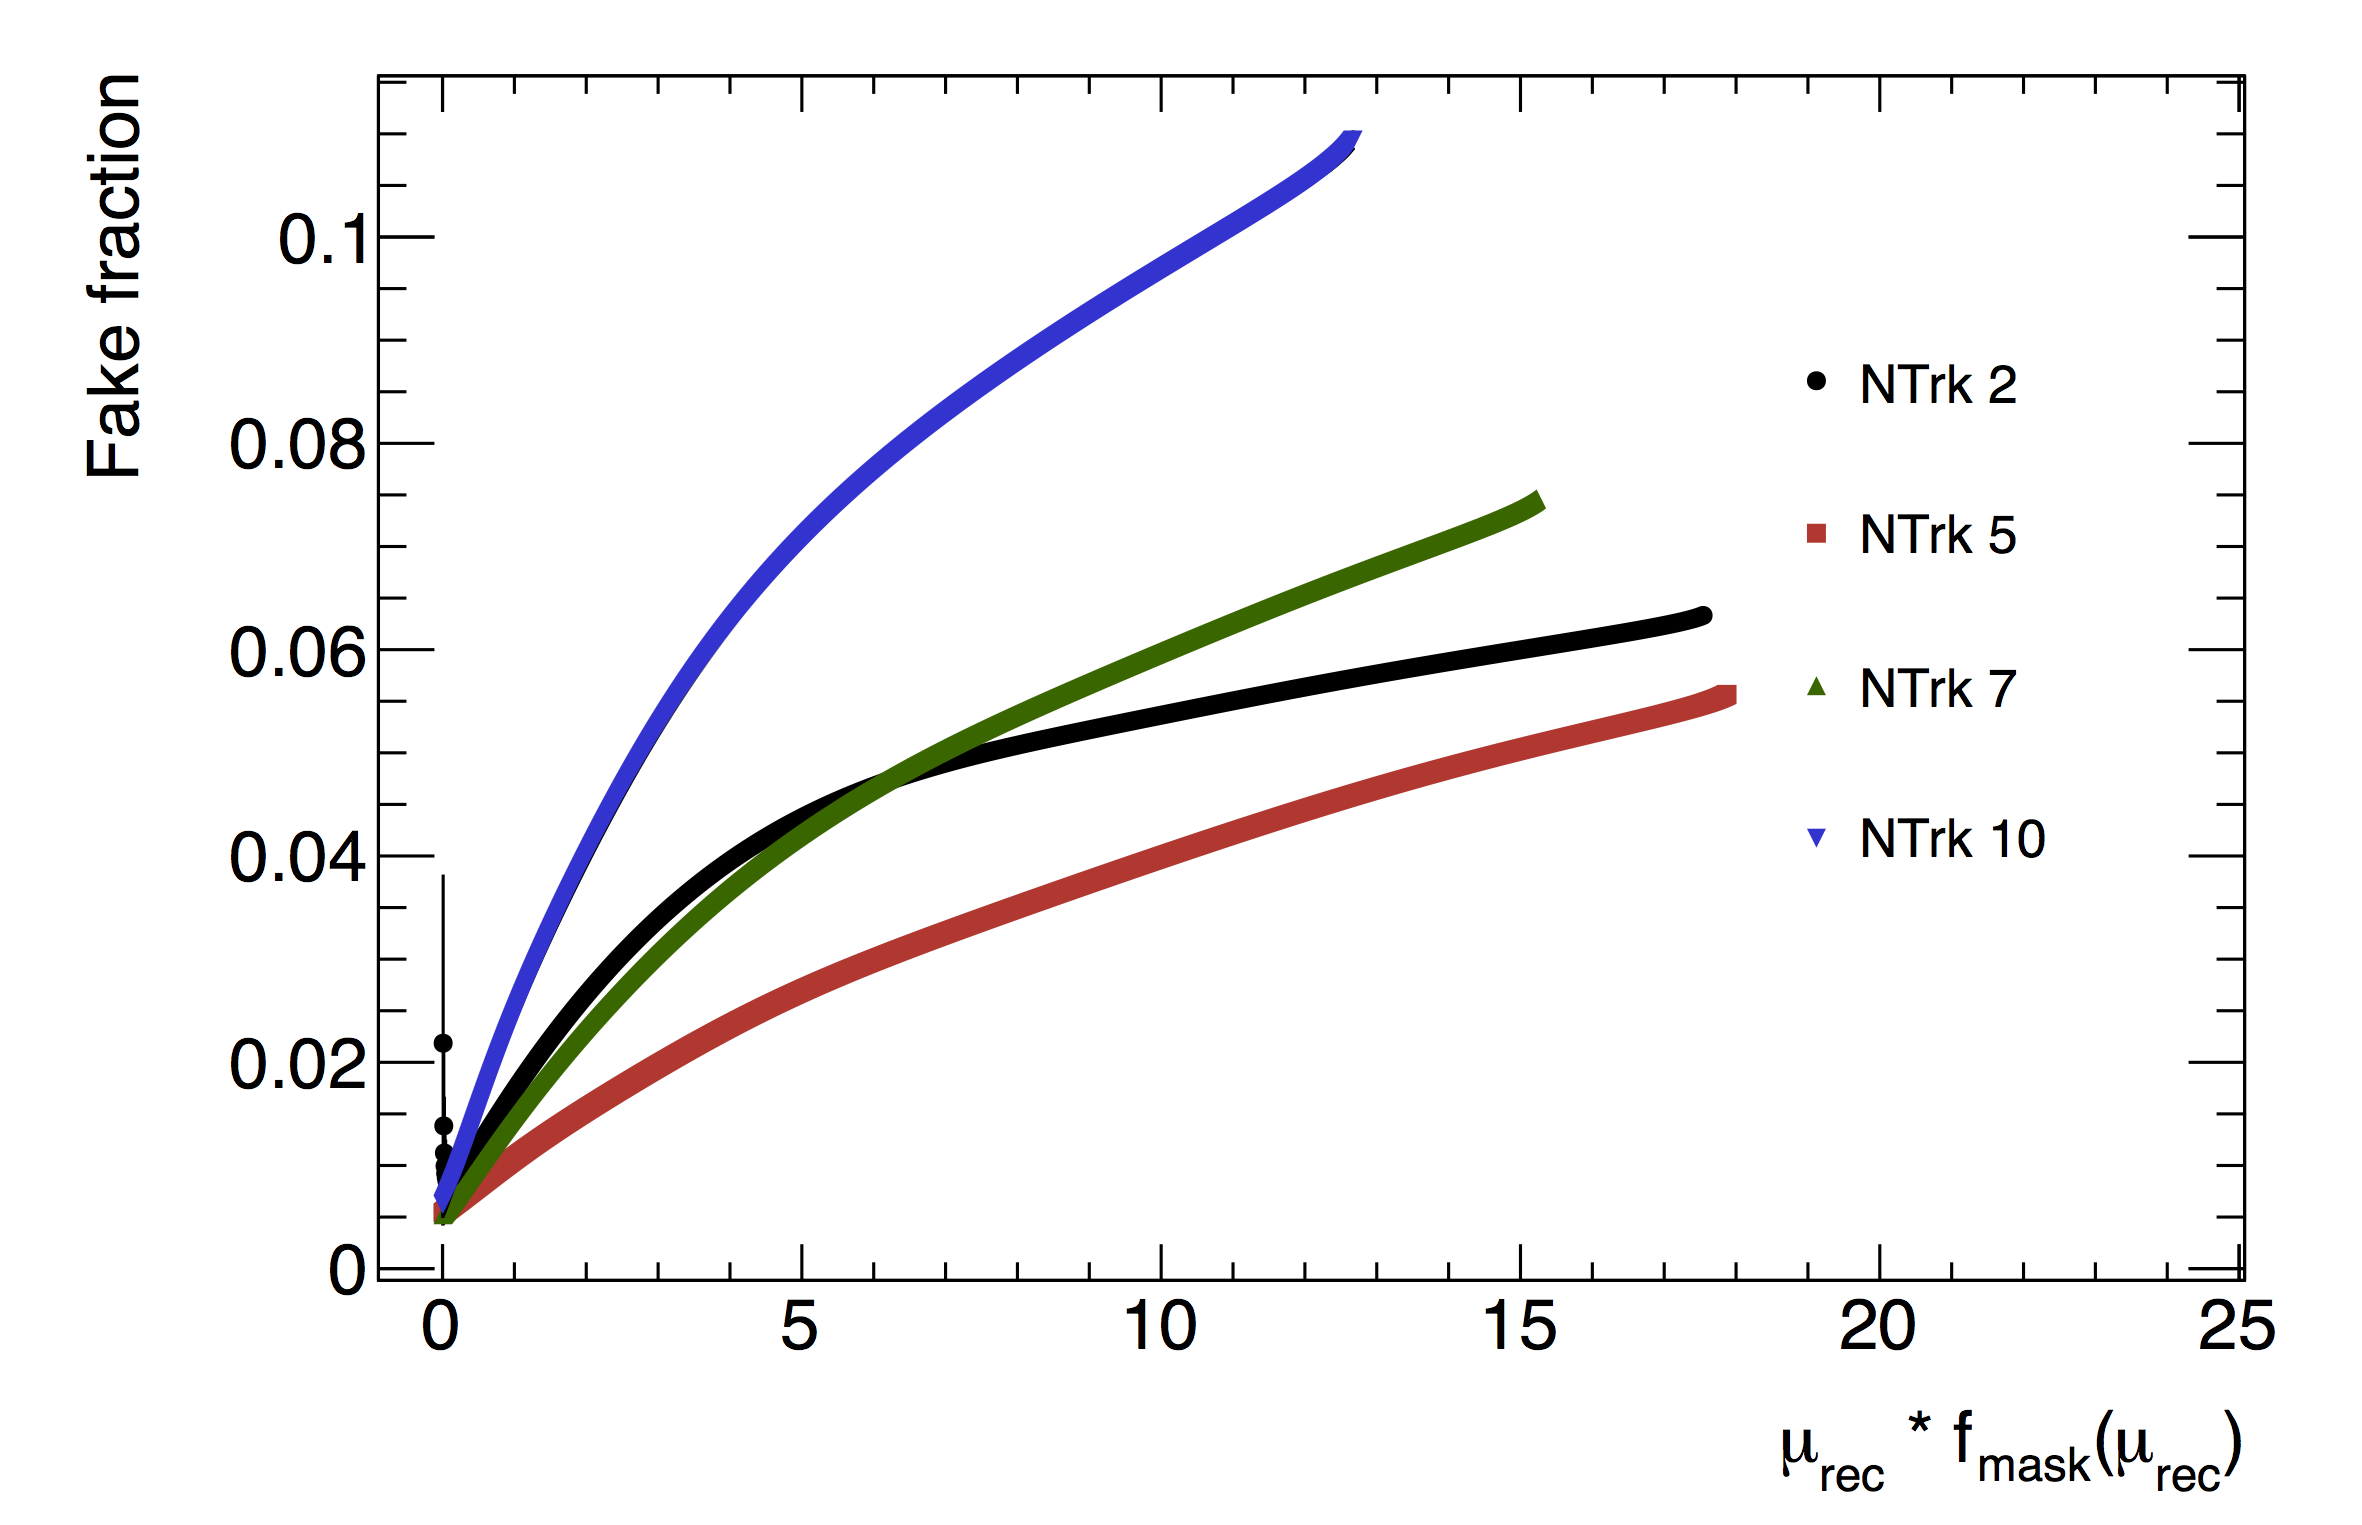
\includegraphics{figures/ch4-reconstruction/c_fake_fraction_MuReconMC.png}}
		\label{fig:fake-fraction-murecmc}
	}
	\caption{Fraction of reconstructed vertices labelled as fake by Monte Carlo truth matching, as a function of pileup.}
	\label{fig:fake-fractions}
\end{figure}


Vertex masking is the dominant effect, causing the large drop in efficiency. Fake vertices are a smaller but significant effect, causing a small increase in the efficiency. Split vertices are a negligible effect once the vertices are required to have at least five tracks. 

A correction procedure is derived for vertex masking using the distribution of longitudinal distances, $\Delta z$, between pairs of vertices in the same event. In the absence of masking, if the interaction region has a Gaussian longitudinal profile with width $\sigma_z$, then the $\Delta z$ distribution would be a Gaussian with width $\sigma_z\times\sqrt{2}$. Masking manifests as an absence of reconstructed pairs near $\Delta z=0$, as shown in figure~\ref{fig:reco-luminosity-deltaz}. 

A correction is derived in a data-driven way as follows. 
\begin{enumerate}
	\item In a data sample with exactly two interactions per event, the number of masked pairs is equal to the number of masked vertices. Using data taken at low pileup values and selecting events with exactly two reconstructed vertices, we calculate the 2-vertex masking probability $p_{\textrm{mask}}(\Delta z)$, i.e. the probability that only one of two vertices separated by $\Delta z$ is reconstructed. This function is assumed to be a universal property of the vertexing algorithm, independent of $\mu$. 
	
	Specifically, the expected $\Delta z$ distribution in the absence of masking, $f_{\mathrm{exp}}(\Delta z)$, is derived by randomly sampling pairs of points from the observed $z$-distribution of reconstructed vertices. Using $f_{\mathrm{exp}}(\Delta z)$ as a template, the \emph{observed} $\Delta z$ distribution, $f_{\mathrm{obs}}(\Delta z)$, is fitted in the range $30$mm$\leq| \Delta z| \leq 300$mm, where vertex masking is negligible. Finally, the masking probability is defined as:
	\begin{equation}
		p_{\textrm{mask}}(\Delta z) = \frac{f_{\mathrm{exp}}(\Delta z) - f_{\mathrm{obs}}(\Delta z)}{f_{\mathrm{exp}}(\Delta z)}
	\end{equation}
	
	The masking probability functions derived from minimum bias Monte Carlo and for low-$\mu$ data are shown in figures~\ref{fig:masking-correction-data} and \ref{fig:masking-correction-mc}.
		
	\item To derive a correction for a particular data sample at arbitrary $\mu$, an \emph{expected} $\Delta z$ distribution, $f_{\mathrm{exp}}(\Delta z)$, is again derived by randomly sample pairs of vertices from the observed primary vertex $z$-distribution. Then, the total probability $p_{\textrm{mask}}$ that given any two tight vertices, only one is reconstructed can be computed: 
	\begin{equation}
		p_{\textrm{mask}} = \int_{-\infty}^{\infty} p_{\textrm{mask}}(\Delta z) f_{\mathrm{exp}}(\Delta z) d(\Delta z).
	\end{equation}
	
	\item The total masking probability $p_{\textrm{mask}}$ is used to generate a map between the number of reconstructible vertices per event, $N_{\textrm{vis}}$, and the average number of reconstructed vertices per event, $\mu_{\textrm{rec}}$, as follows. Label the generated vertices $v_i$, $1 \leq i \leq N_{gen}$, in the order in which the iterative vertexing algorithm reconstructs the vertices; similarly, let $p_i$, $1\leq i \leq N_{\textrm{vis}}$, be the probability that vertex $v_i$ is reconstructed. Proceeding vertex-by-vertex, the $p_i$ follow a recursion relation:

	\begin{align}
		p_1 &= 1\\
		p_2 &= p_1 \times (1 - p_{\textrm{mask}})\\
		&... \\
		p_k &= \prod_{i=1}^{k-1} \left( p_i  \times (1-p_{\textrm{mask}}) + (1-p_i) \times 1\right)\\
		&= \prod_{i=1}^{k-1} \left(1 - p_i p_{\textrm{mask}}\right)\\
		&= p_{n-1} \times \left(1-p_{n-1} p_{\textrm{mask}}\right)
	\end{align}
	The average number of reconstructed vertices is then:
	\begin{align}
		\langle N_{\textrm{rec}} \rangle &= \sum_{i=1}^{N_{\textrm{vis}}} p_i.
	\end{align}
	
	\item Finally, a map is computed between the average number of reconstructible vertices, $\mu_{\textrm{vis}}$, and the average number of reconstructed vertices, $ \mu_{\textrm{rec}}(\mu_{\textrm{vis}})$, by convoluting $\mu_{\textrm{rec}}(N_{\textrm{vis}})$ with a Poisson distribution:
	\begin{align}
		\langle \mu_{\textrm{rec}} \rangle (\mu_{\textrm{vis}}) = \sum_{N_{\textrm{vis}}=0}^{\infty} P(N_{\textrm{vis}}; \mu_{\textrm{vis}}) \mu_{\textrm{rec}} (N_{\textrm{vis}}).
	\end{align}
\end{enumerate}

\begin{figure}[p]
	\centering
	\subfloat[$\Delta z$ distribution and template fit, NTrk5, BCID 81] {
		\resizebox{3in}{!}{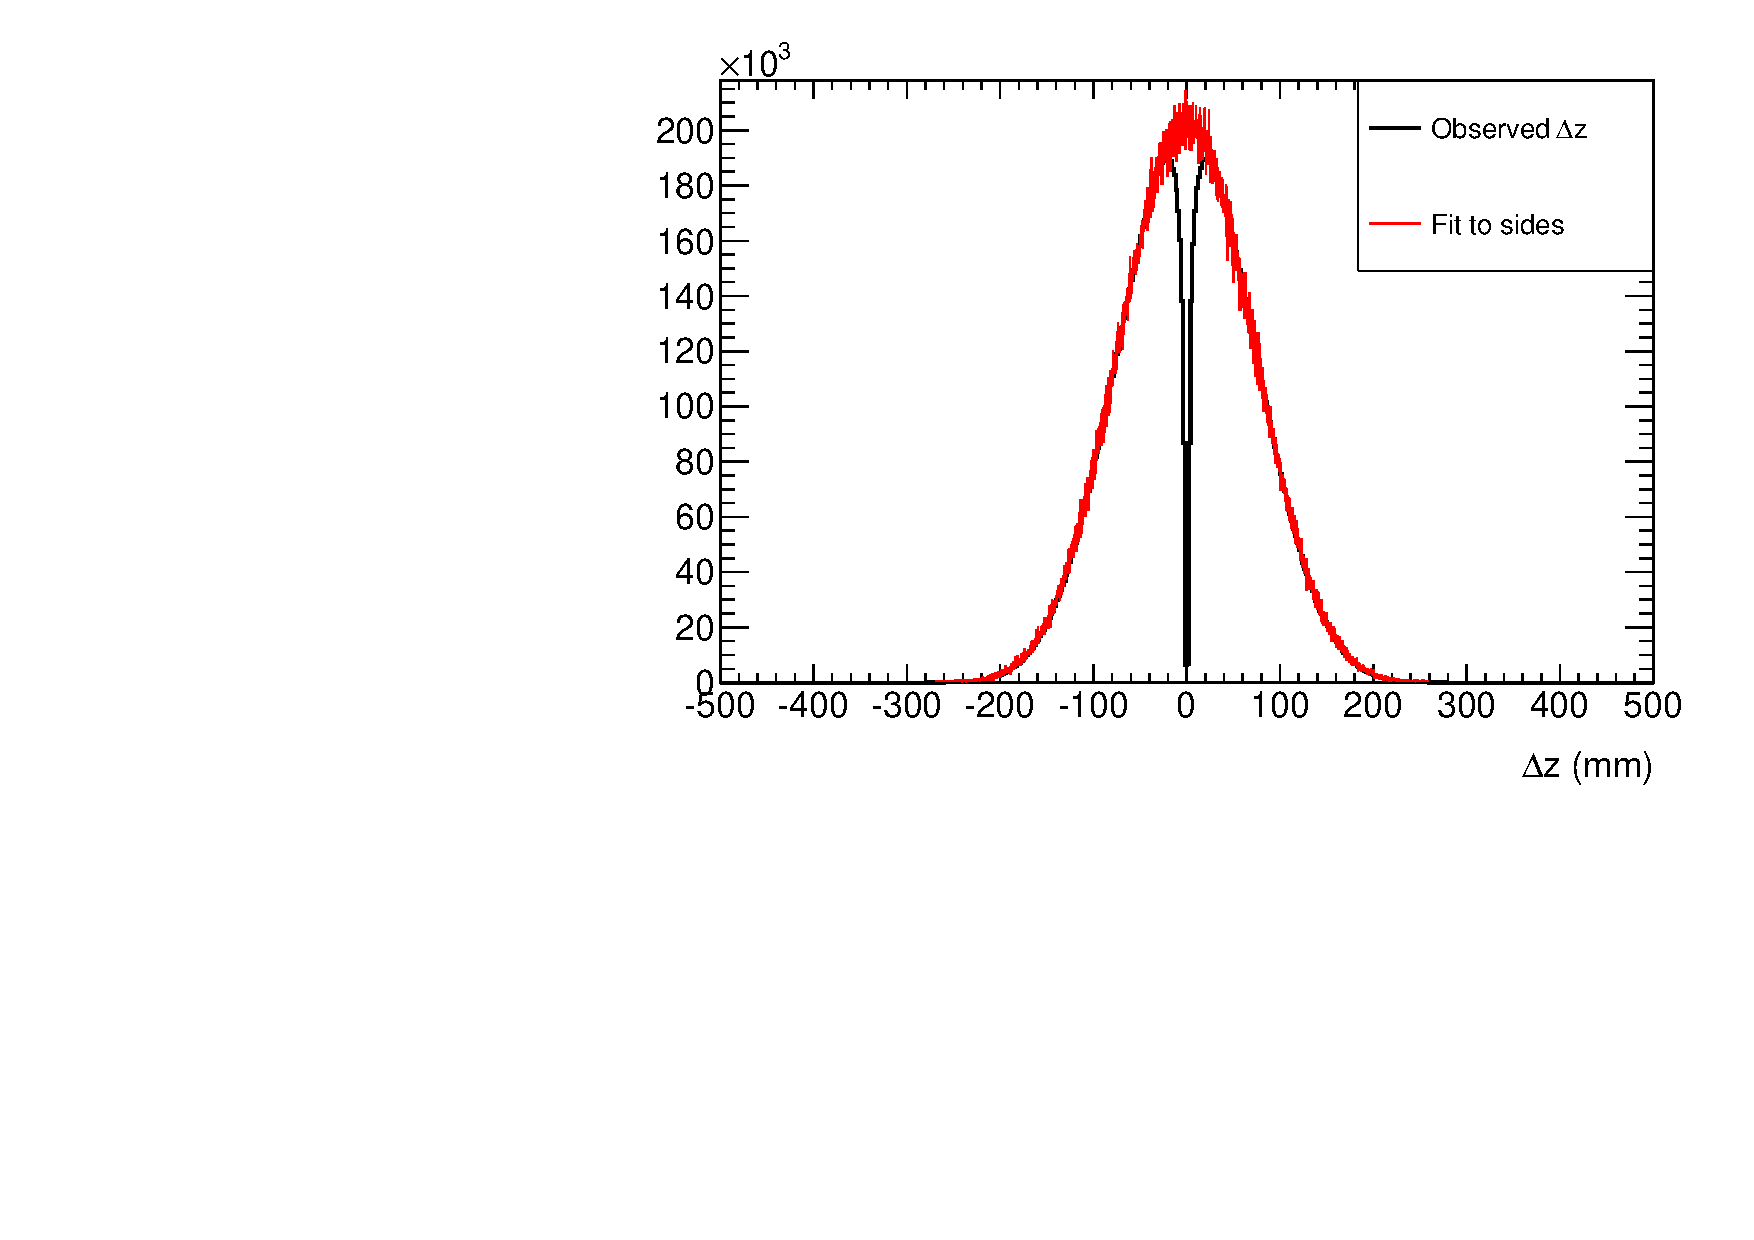
\includegraphics{figures/ch4-reconstruction/c_dz_NTrk5_BCID81}}
	}
	\subfloat[$p_{\textrm{mask}}(\Delta z)$, NTrk5] {
		\resizebox{3in}{!}{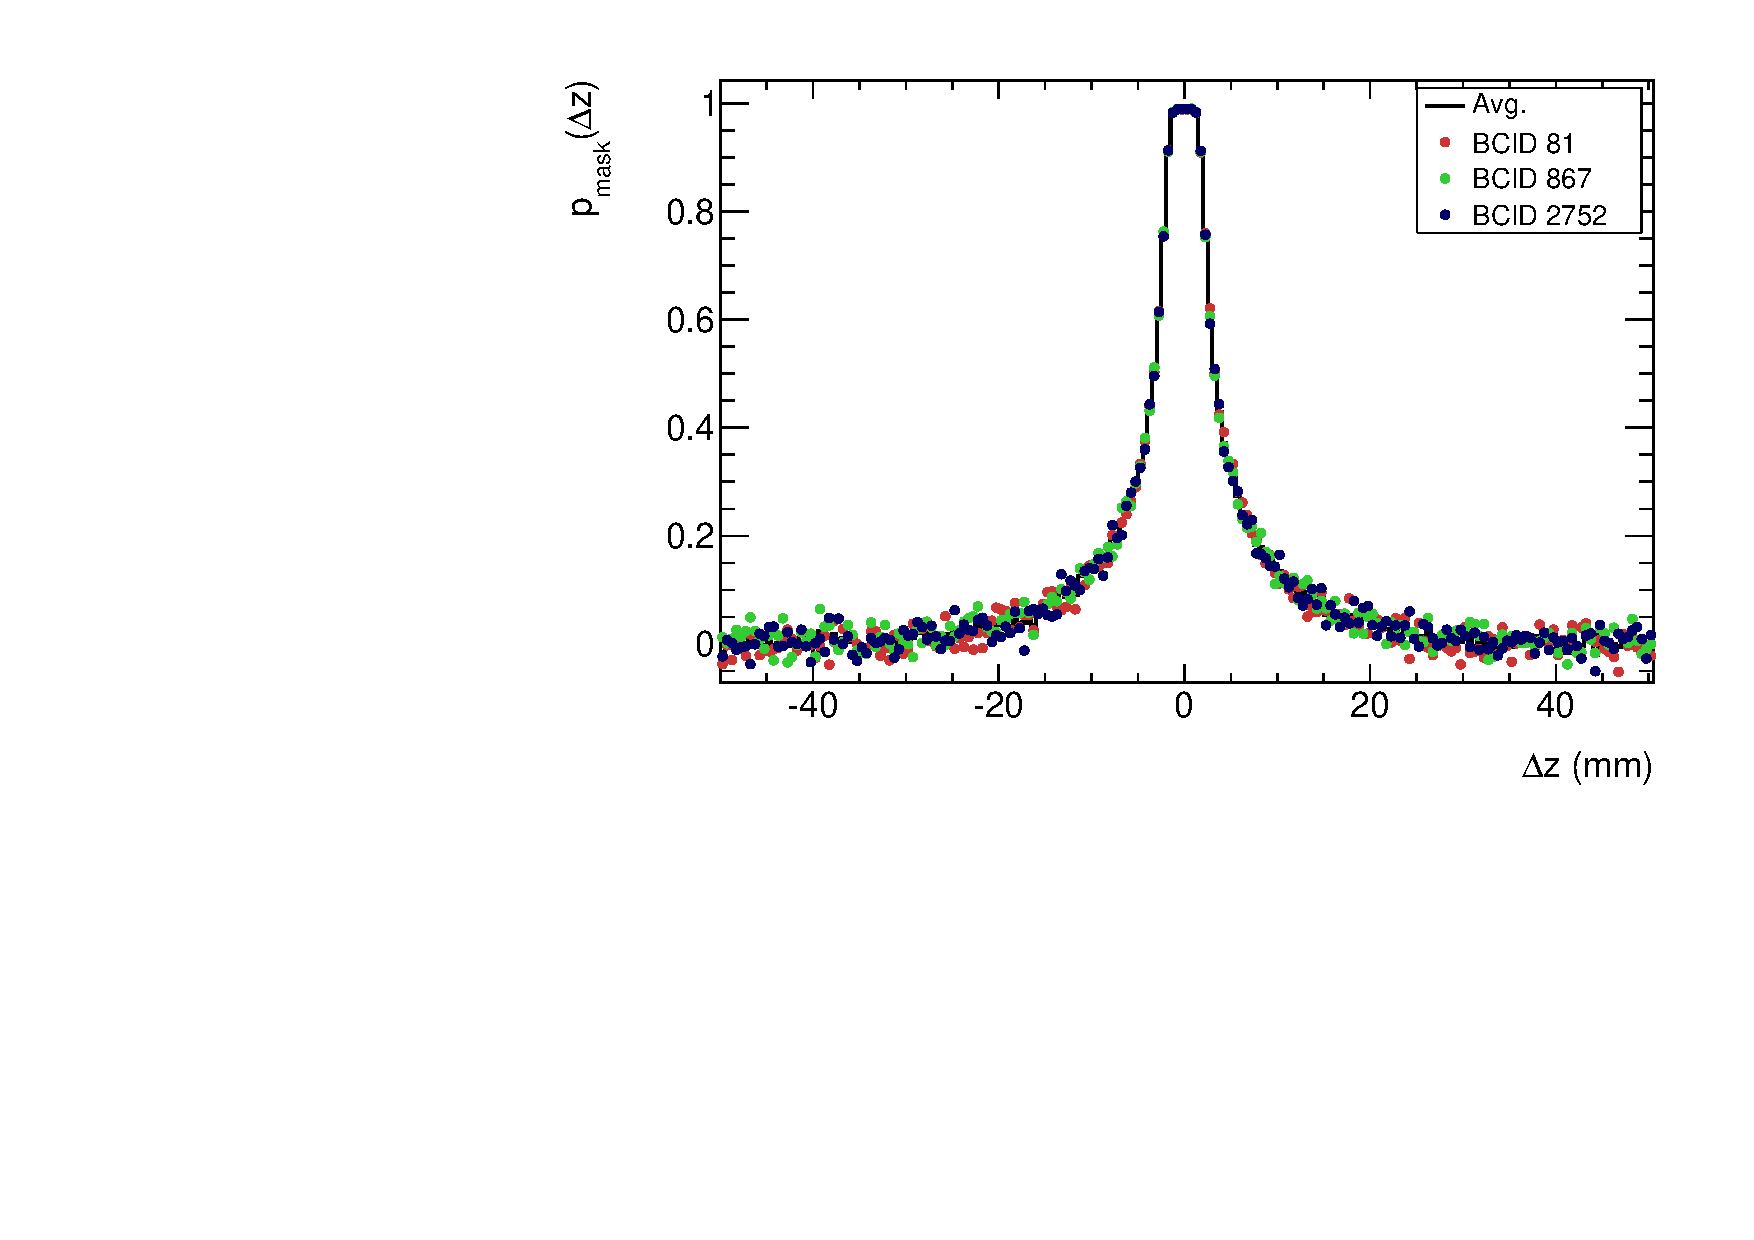
\includegraphics{figures/ch4-reconstruction/c_pmask_dz_NTrk5}}
	}\\
	\subfloat[$\Delta z$ distribution and template fit, NTrk7, BCID 81] {
		\resizebox{3in}{!}{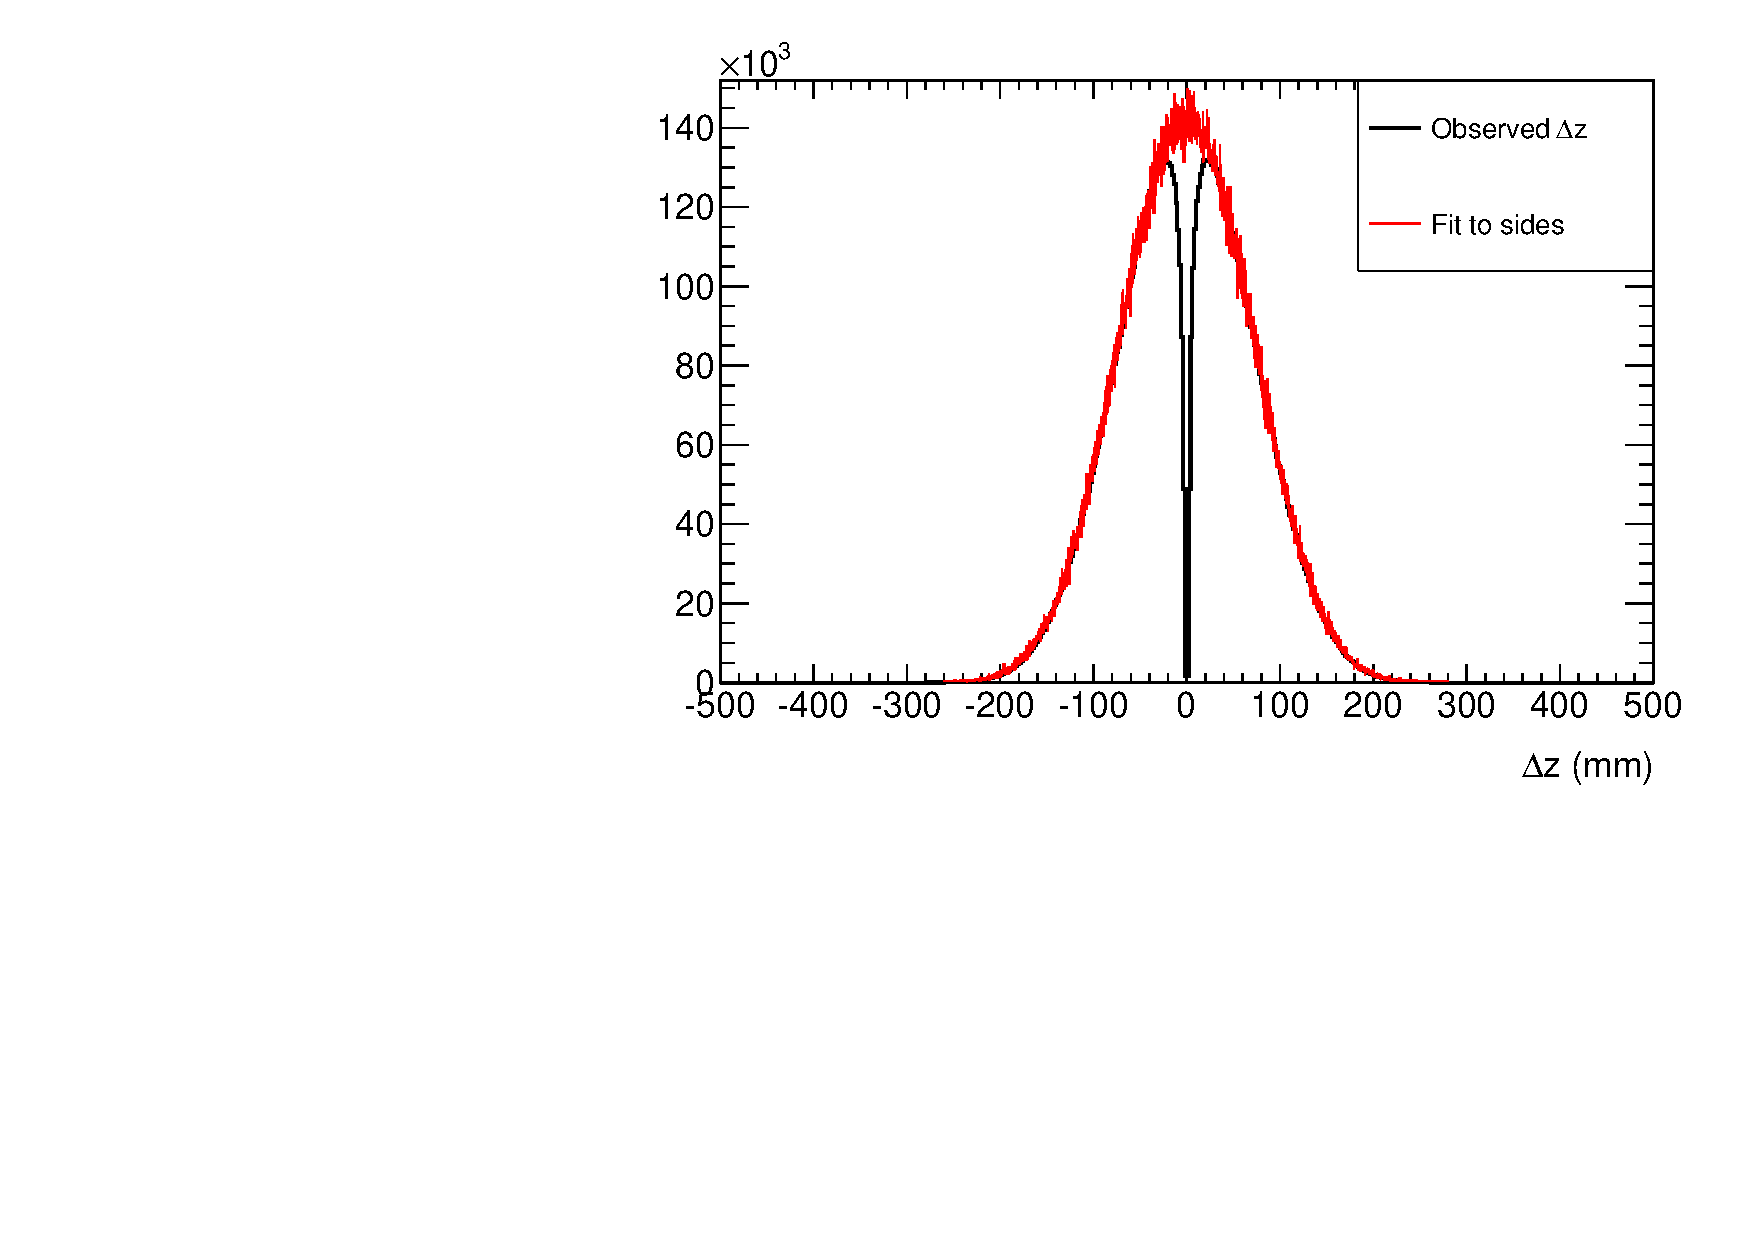
\includegraphics{figures/ch4-reconstruction/c_dz_NTrk7_BCID81}}
	}
	\subfloat[$p_{\textrm{mask}}(\Delta z)$, NTrk7] {
		\resizebox{3in}{!}{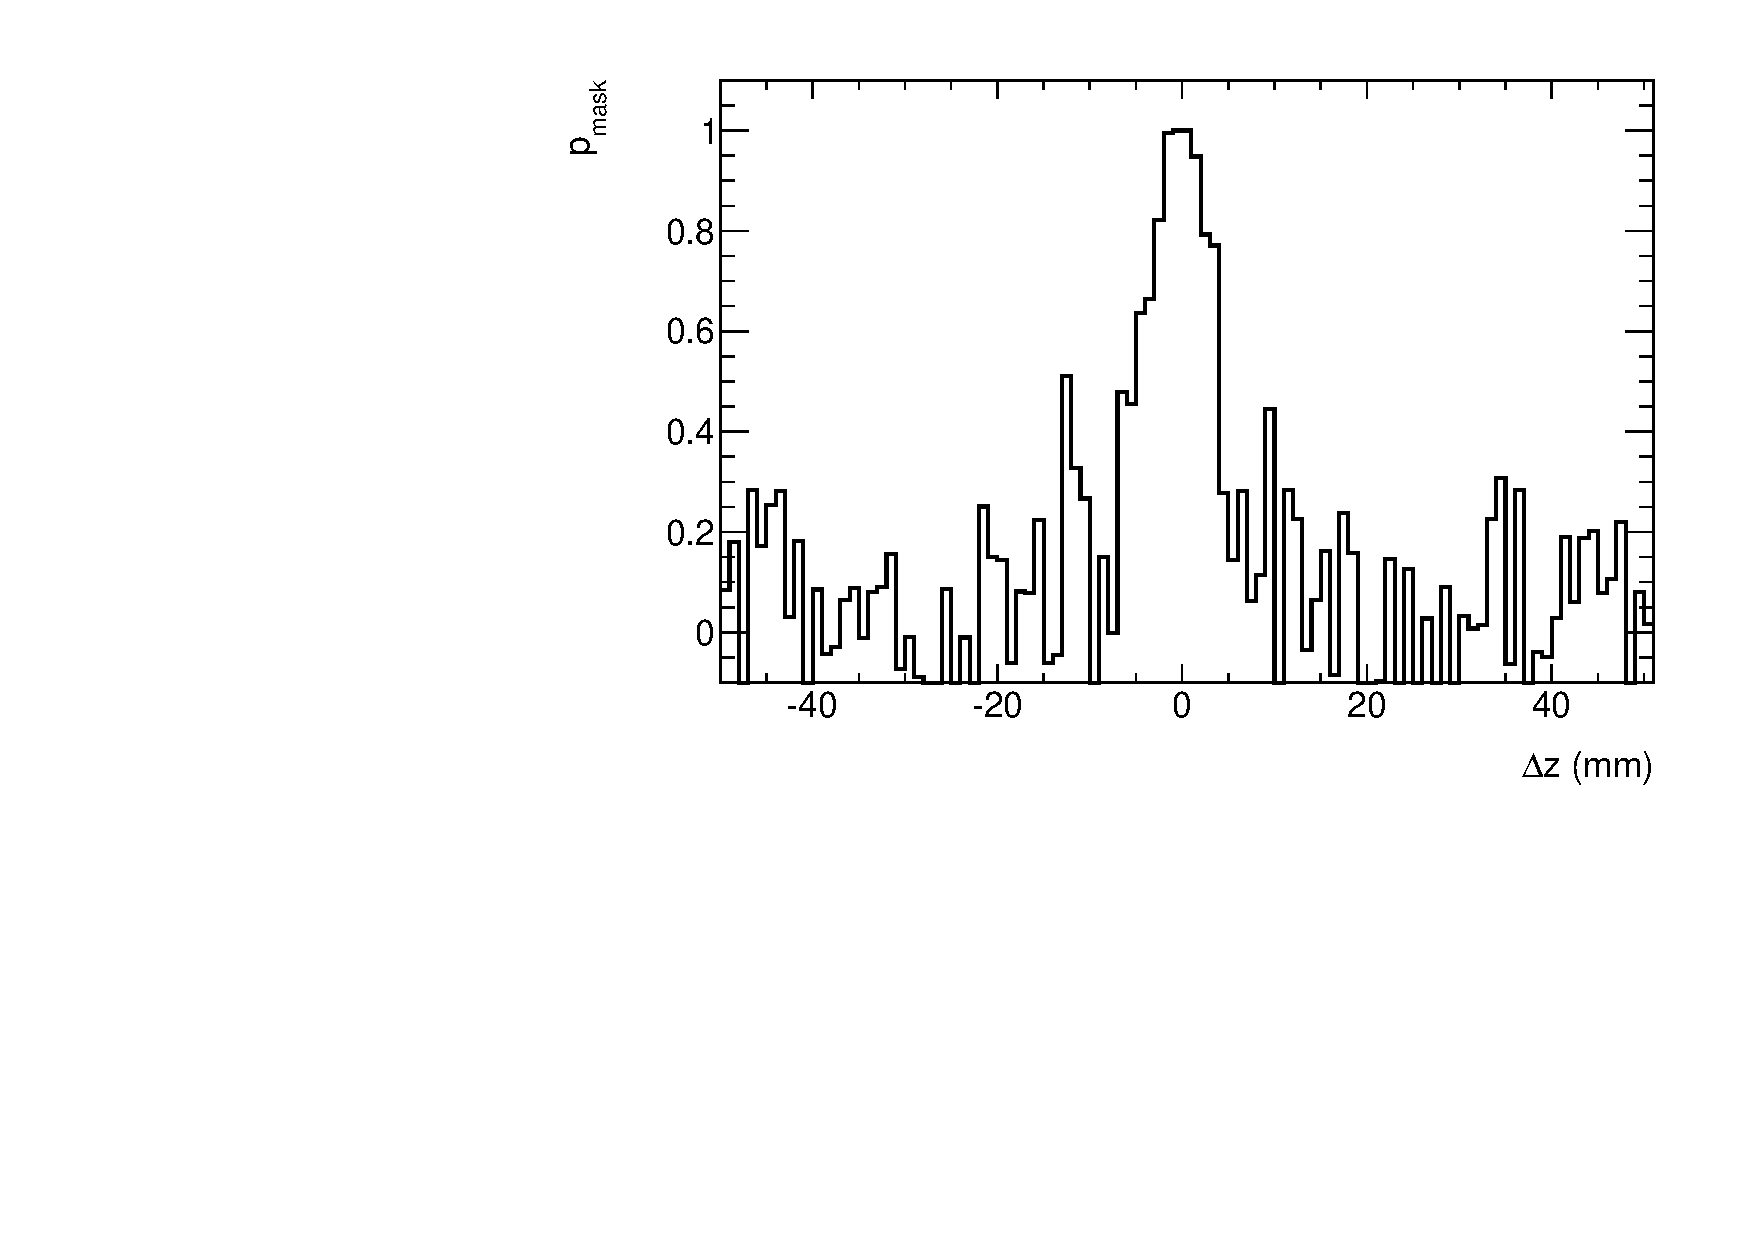
\includegraphics{figures/ch4-reconstruction/c_pmask_dz_NTrk7}}
	}\\
	\subfloat[$\Delta z$ distribution and template fit, NTrk10, BCID 81] {
		\resizebox{3in}{!}{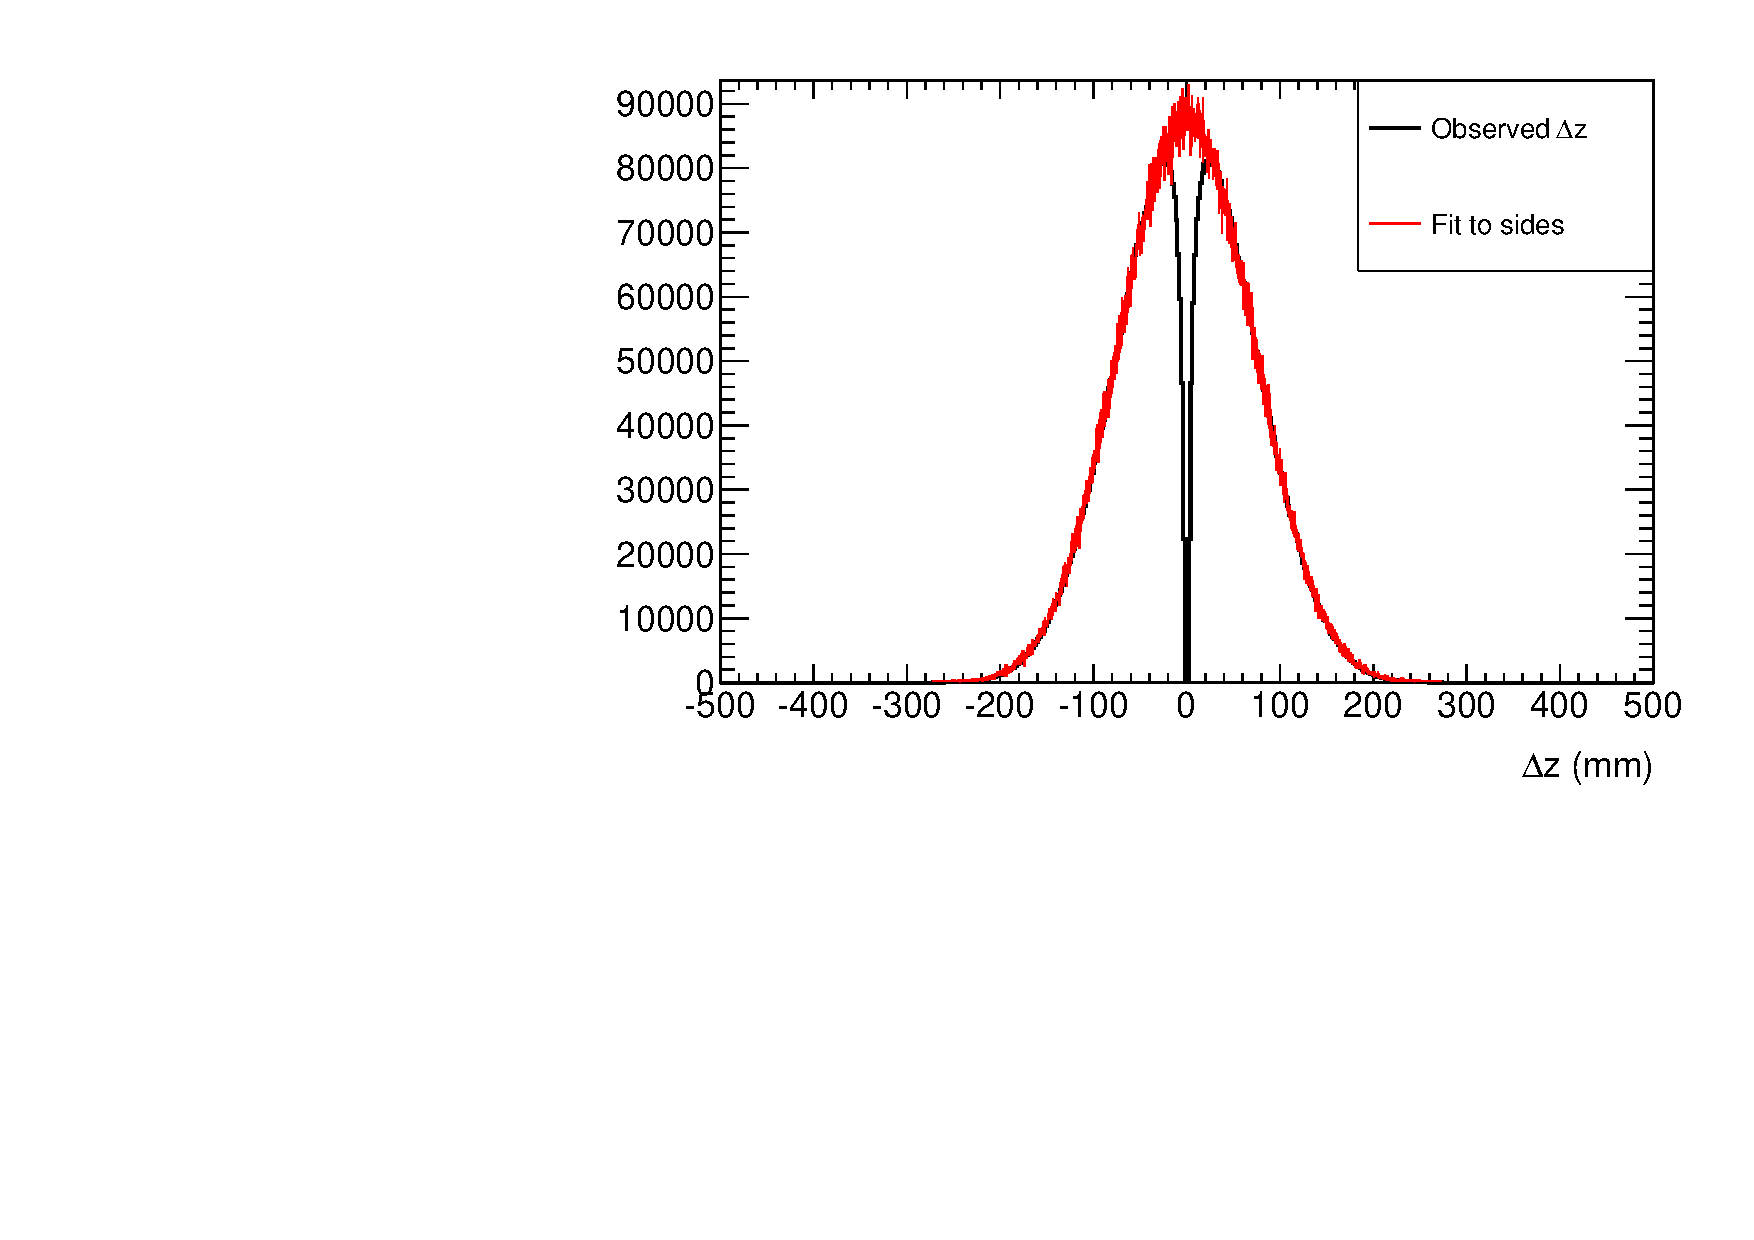
\includegraphics{figures/ch4-reconstruction/c_dz_NTrk10_BCID81}}
	}
	\subfloat[$p_{\textrm{mask}}(\Delta z)$, NTrk10] {
		\resizebox{3in}{!}{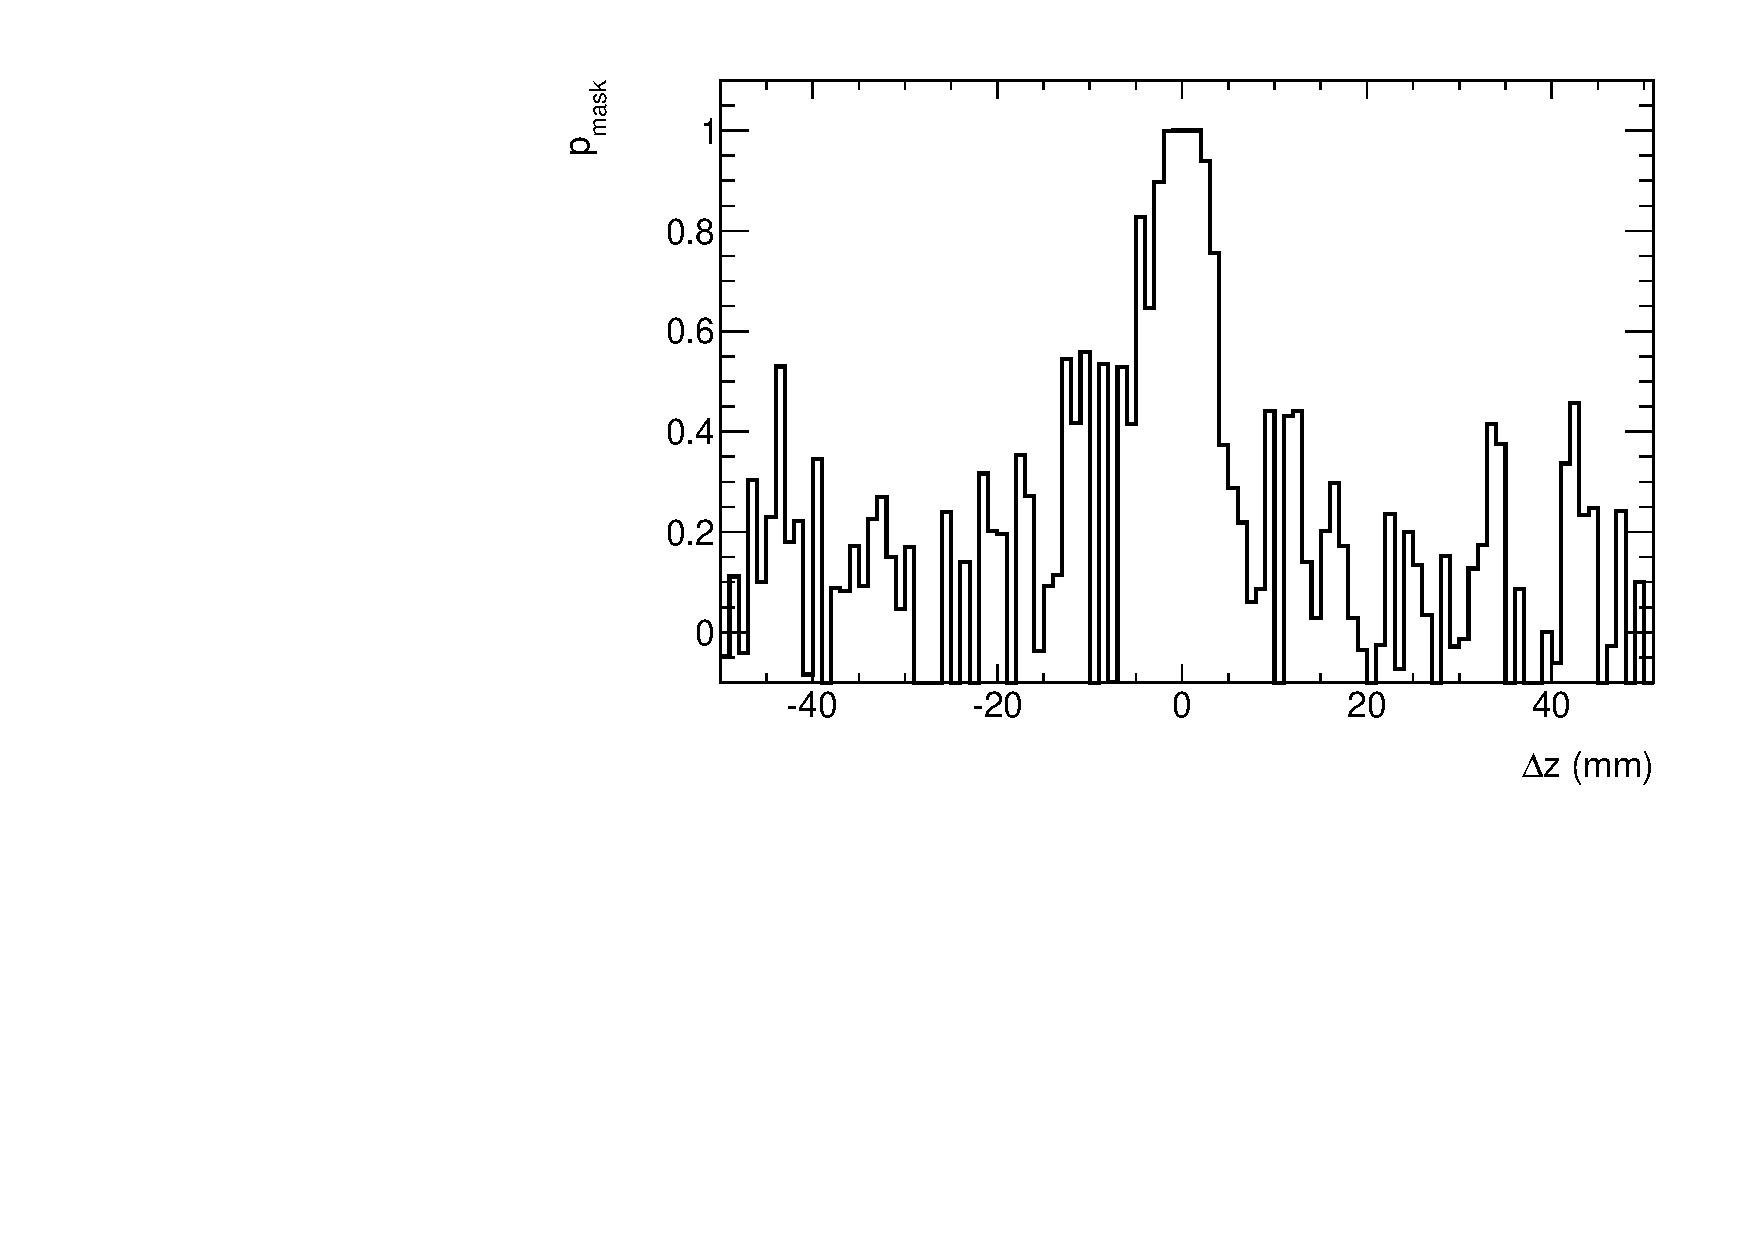
\includegraphics{figures/ch4-reconstruction/c_pmask_dz_NTrk10}}
	}\\
	\caption{Calibration of the masking correction method on data, using run 182013. Left: $\Delta z$ distributions and template fits using expected $\Delta z$ distributions in the range $30$~mm$\leq\Delta z\leq300$~mm. Right: pairwise vertex masking probability as a function of the longitudinal distance $\Delta z$ between the vertices.}
	\label{fig:masking-correction-data}
\end{figure}

\begin{figure}[p]
	\centering
	\subfloat[$\Delta z$ distribution and template fit, NTrk5] {
		\resizebox{3in}{!}{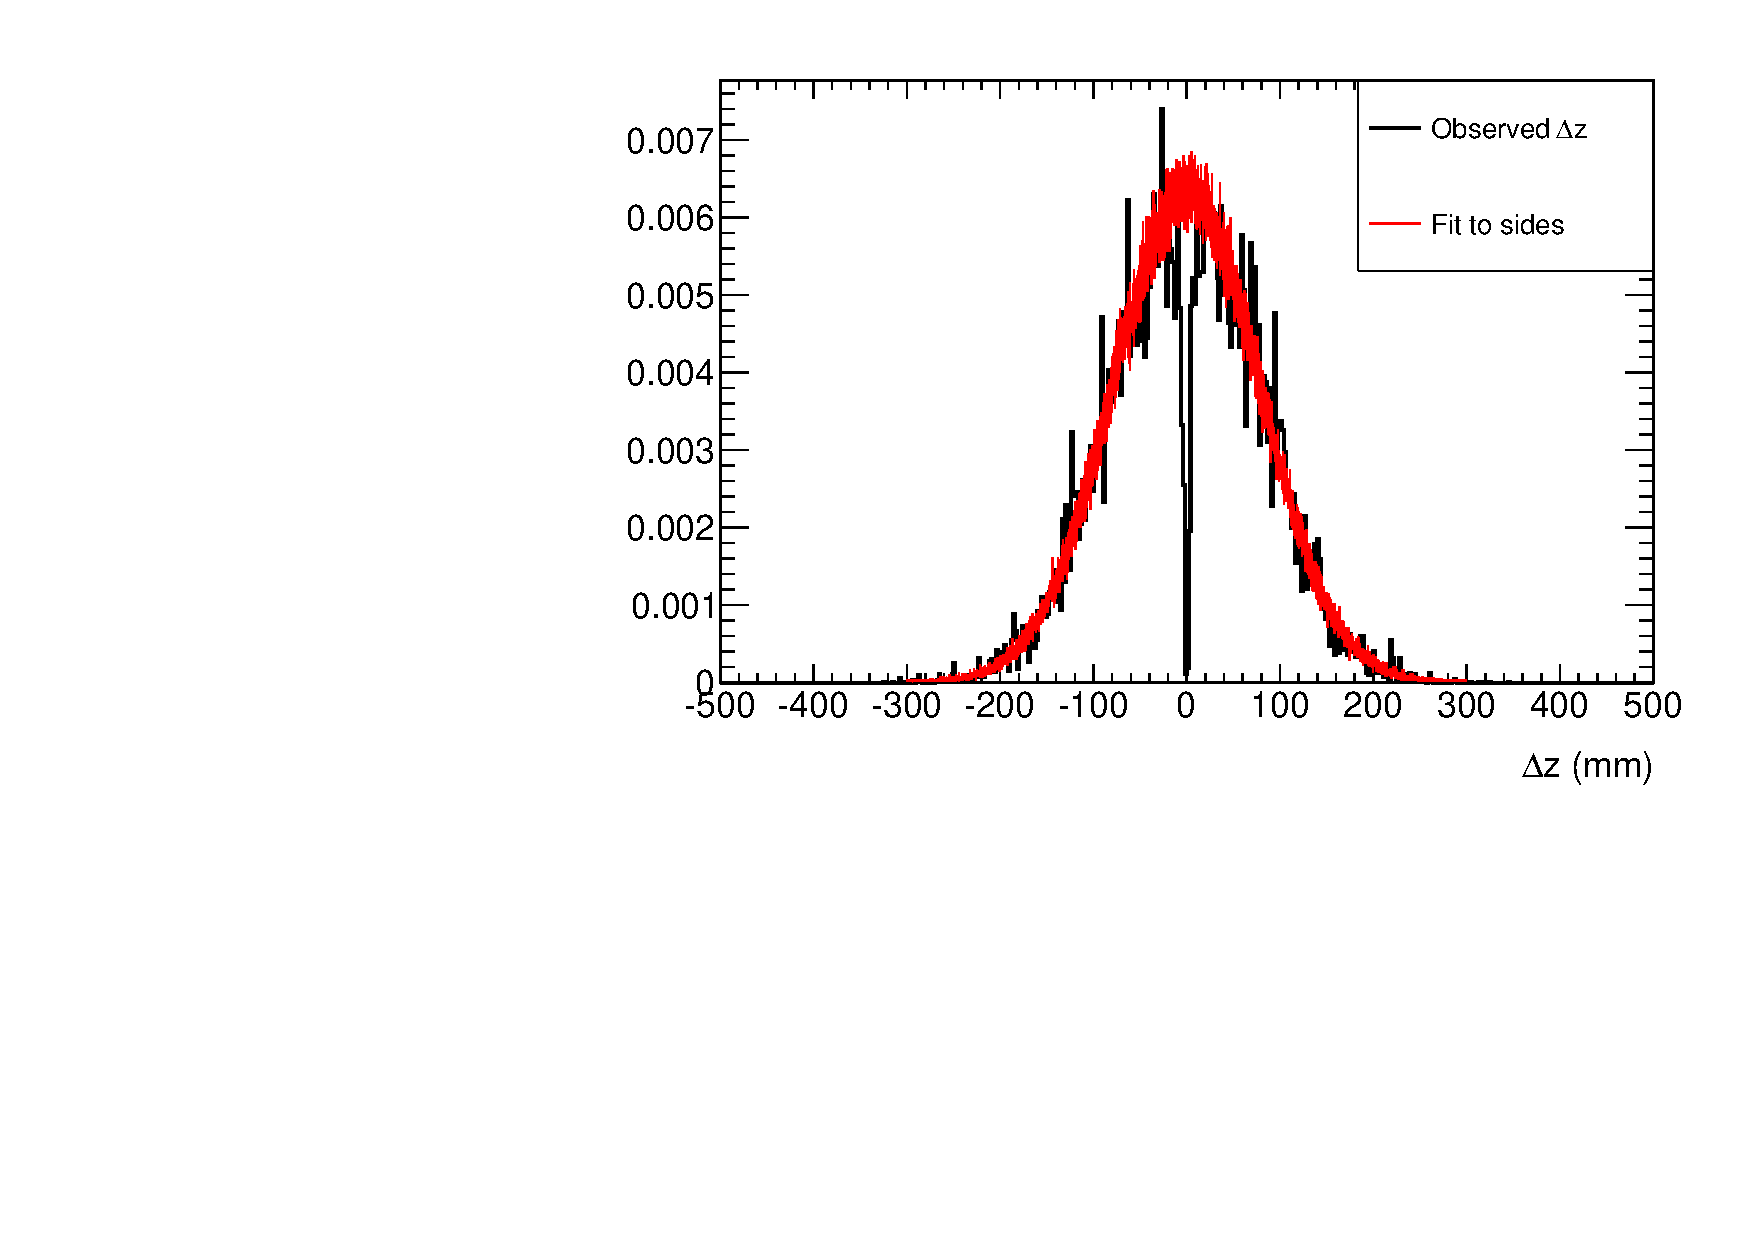
\includegraphics{figures/ch4-reconstruction/c_dz_NTrk5}}
	}
	\subfloat[$p_{\textrm{mask}}(\Delta z)$, NTrk5] {
		\resizebox{3in}{!}{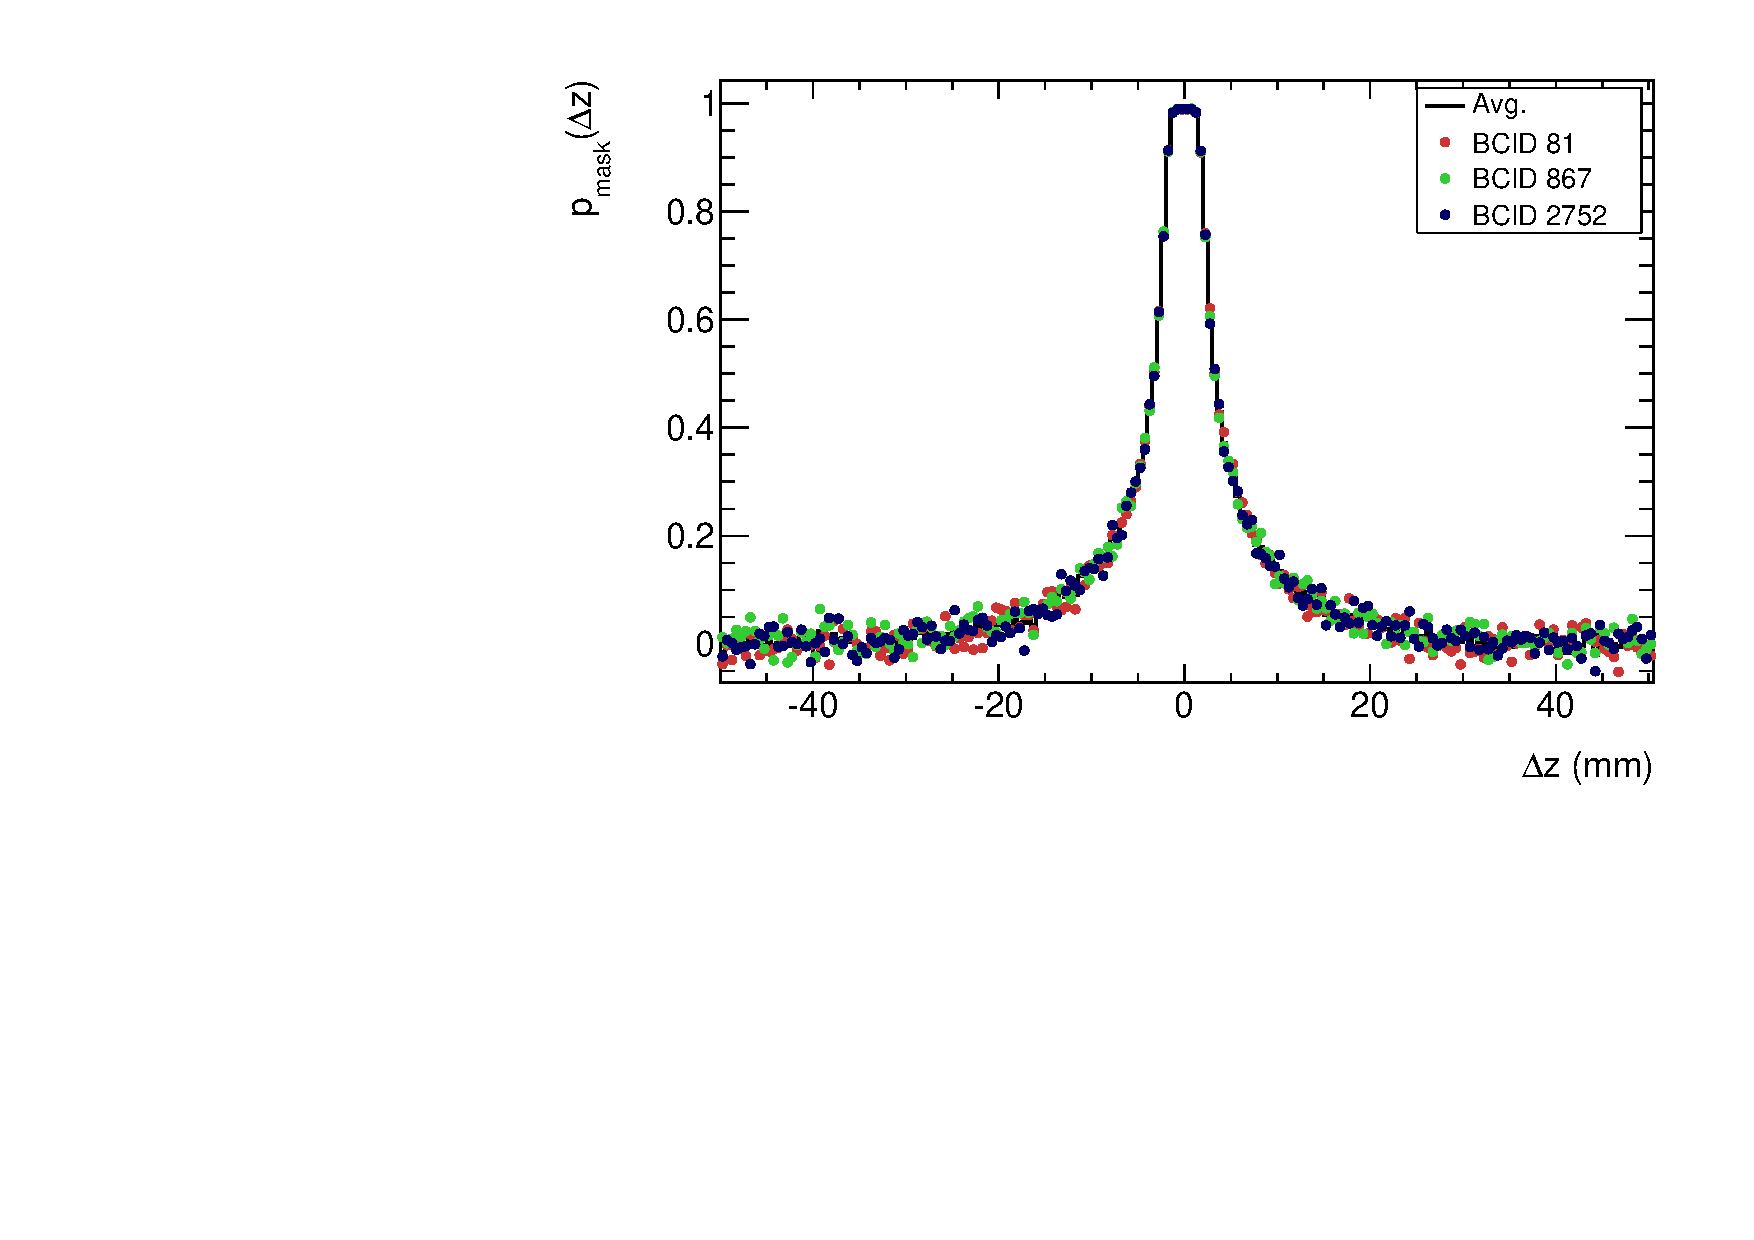
\includegraphics{figures/ch4-reconstruction/c_pmask_dz_NTrk5}}
	}\\
	\subfloat[$\Delta z$ distribution and template fit, NTrk7] {
		\resizebox{3in}{!}{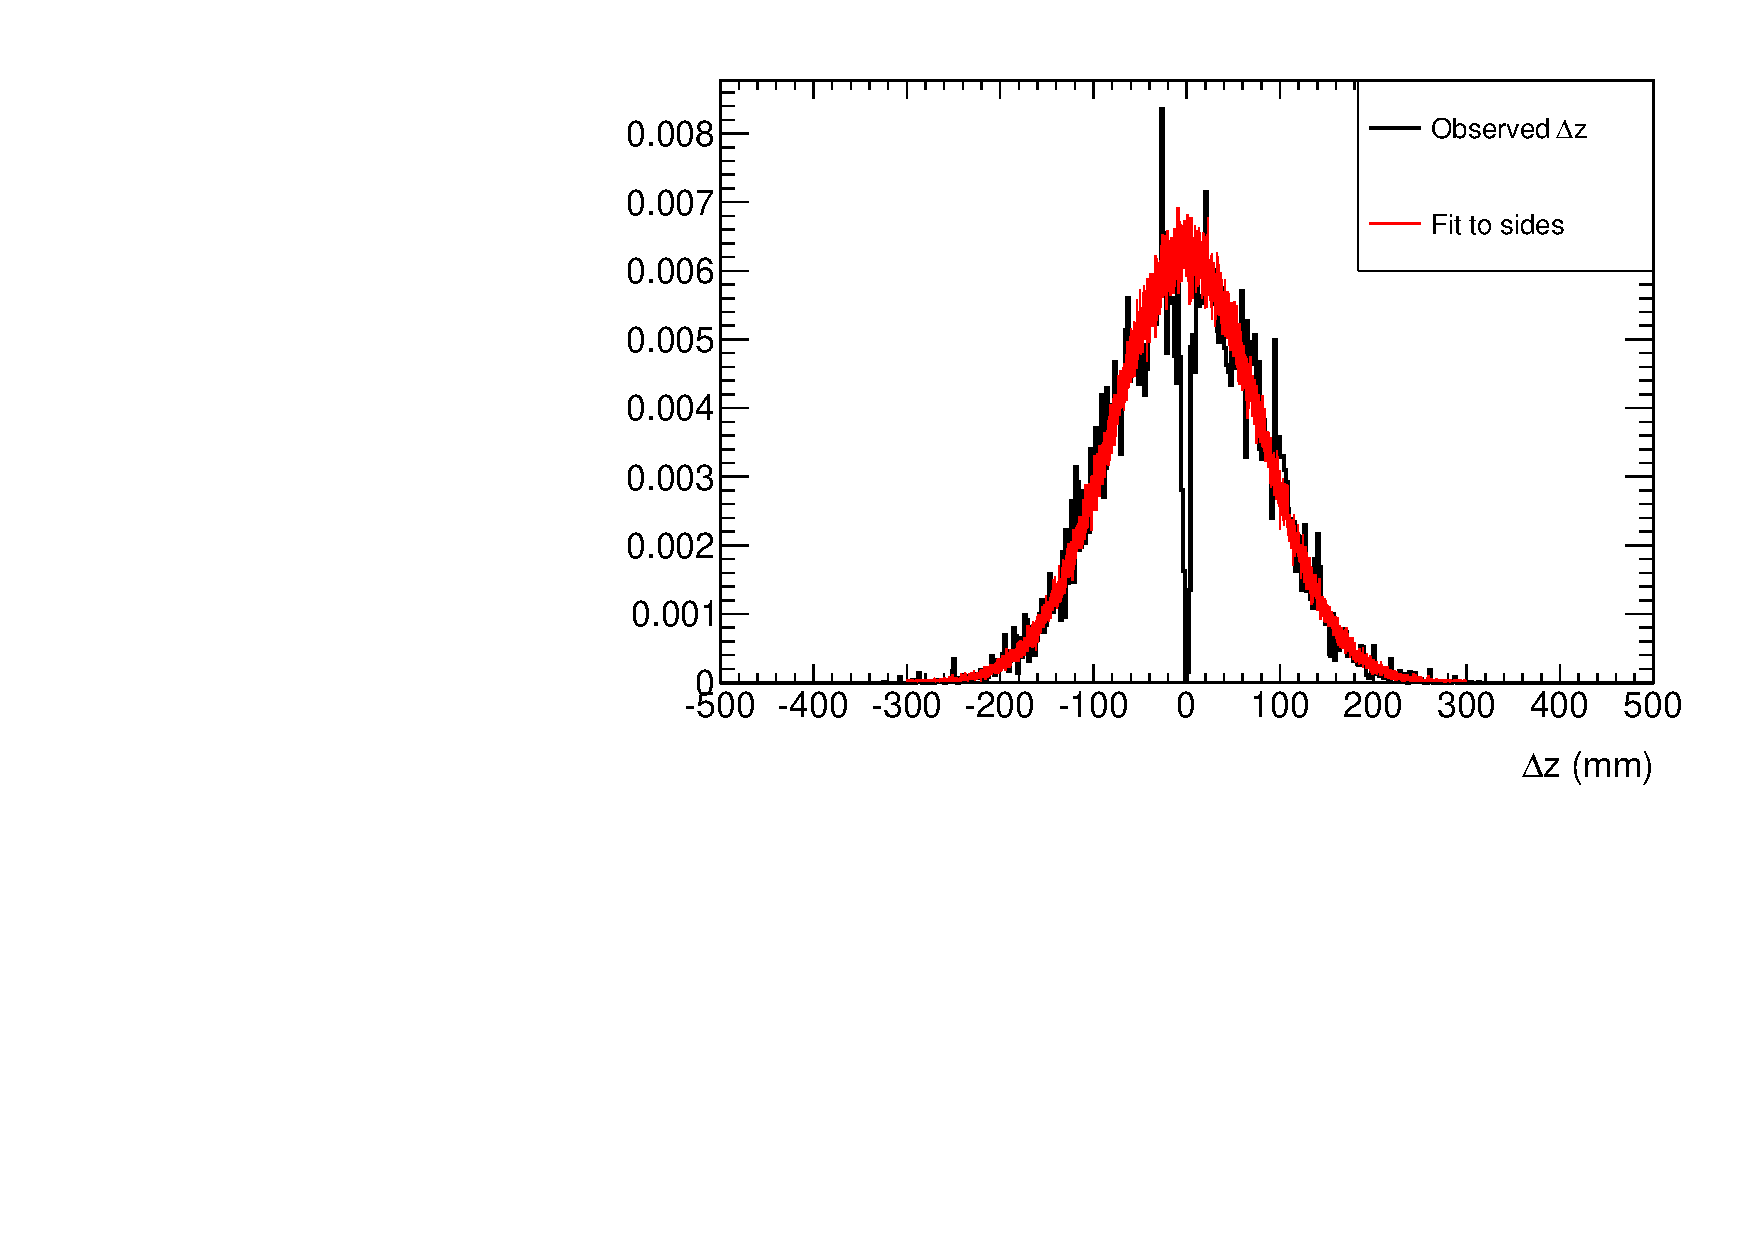
\includegraphics{figures/ch4-reconstruction/c_dz_NTrk7}}
	}
	\subfloat[$p_{\textrm{mask}}(\Delta z)$, NTrk7] {
		\resizebox{3in}{!}{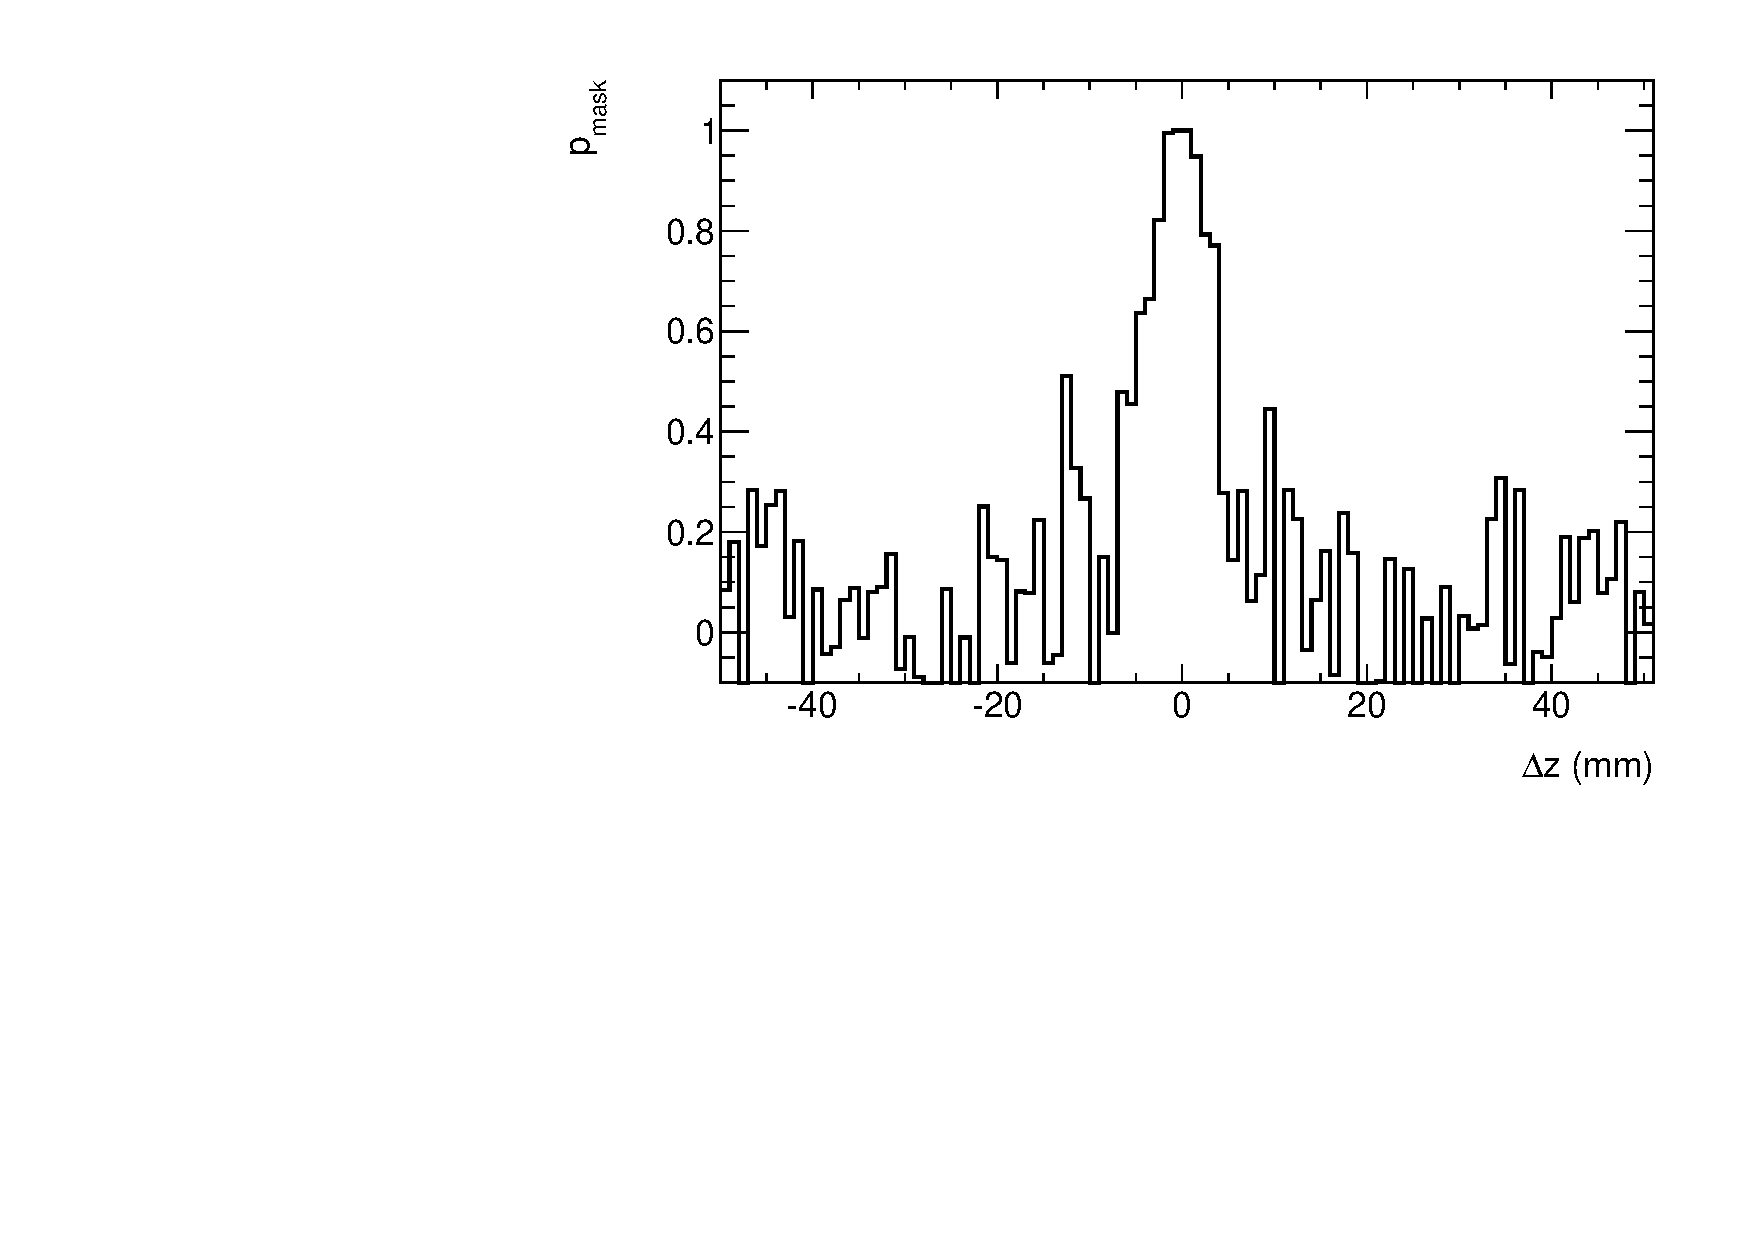
\includegraphics{figures/ch4-reconstruction/c_pmask_dz_NTrk7}}
	}\\
	\subfloat[$\Delta z$ distribution and template fit, NTrk10] {
		\resizebox{3in}{!}{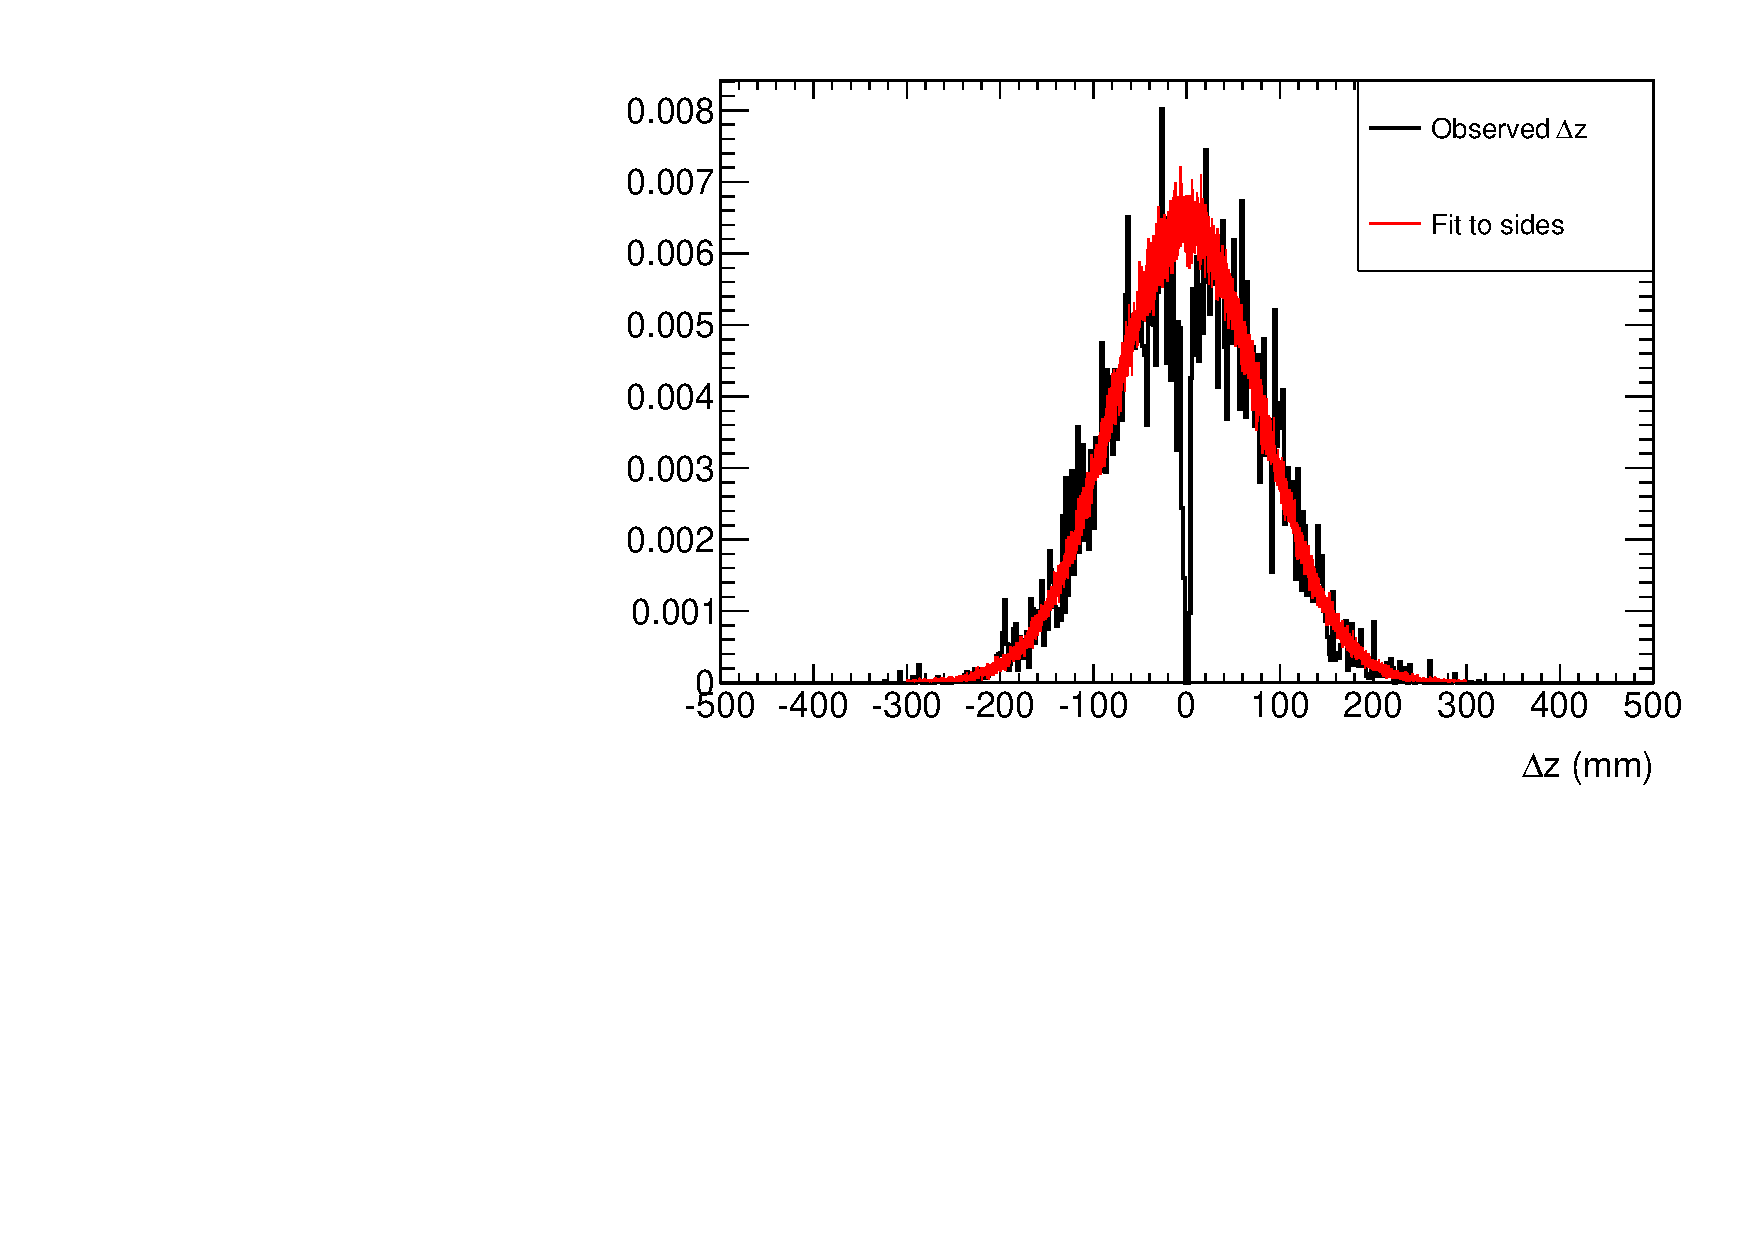
\includegraphics{figures/ch4-reconstruction/c_dz_NTrk10}}
	}
	\subfloat[$p_{\textrm{mask}}(\Delta z)$, NTrk10] {
		\resizebox{3in}{!}{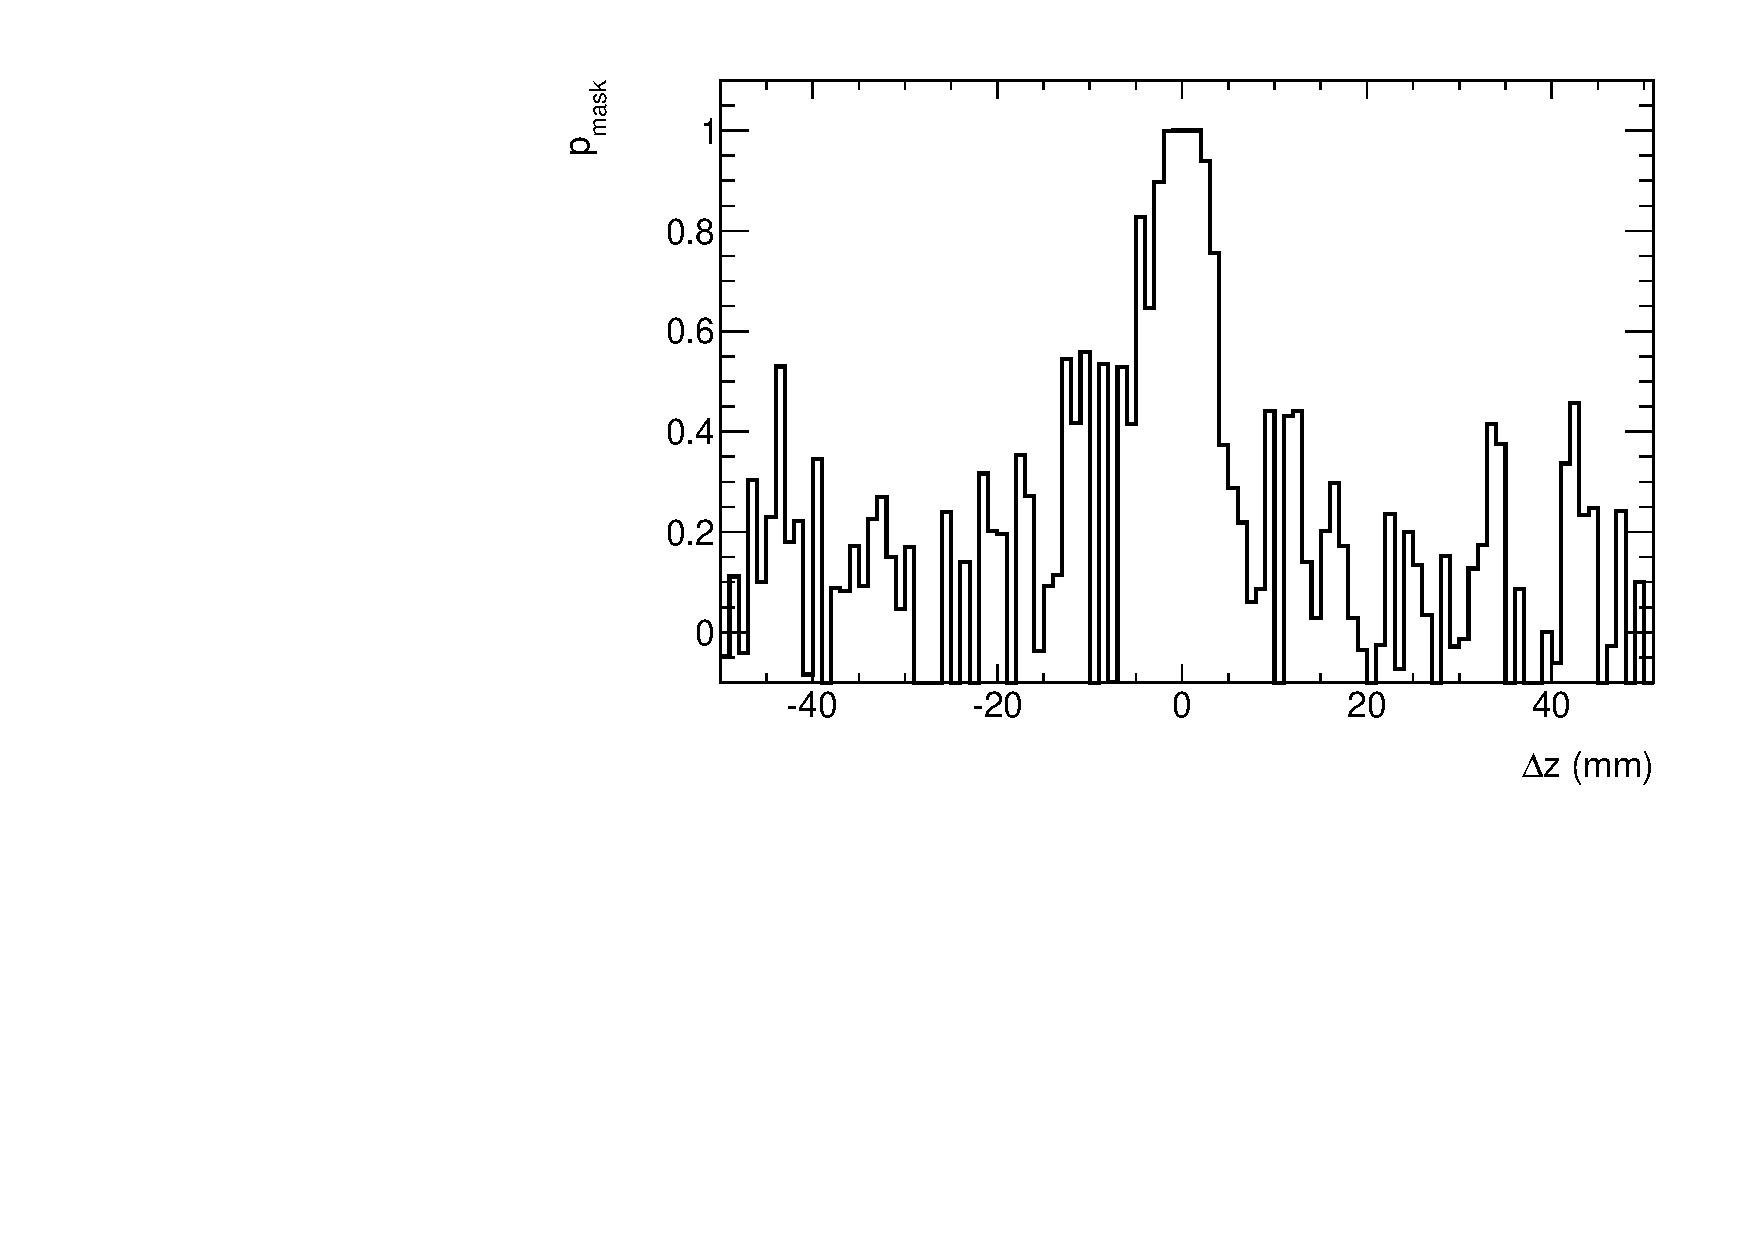
\includegraphics{figures/ch4-reconstruction/c_pmask_dz_NTrk10}}
	}\\
	\caption{Calibration of the masking correction method on simulation, using 8~TeV minimum bias Monte Carlo (pythia 8, tune A2M). Left: $\Delta z$ distributions and template fits using expected $\Delta z$ distributions in the range $30$~mm$\leq\Delta z\leq300$~mm. Right: pairwise vertex masking probability as a function of the longitudinal distance $\Delta z$ between the vertices.}
	\label{fig:masking-correction-mc}
\end{figure}

\subsubsection{Vertex-Based Luminosity Measurements}
Due to the low event rate available during physics runs, vertex counting was used to measure luminosity only in three special runs during 2011, where inner detector data was recorded by a special high-rate data stream. The data stream reads out events at $\mathcal{O}(10~\mbox{kHz}$, recording only the inner detector from a small number of bunch crossings, typically less than four. The three runs are the vdM calibration run in May 2011, the pileup scan in September 2011 shown in figure~\ref{fig:reco-luminosity-comparisons-pileup}, and a high-$\beta^{*}$ run with a single bunch used to measure the total $pp$ cross section using the ALFA detector. 

\ 

\textbf{Van der Meer Scan}

An example scan curve from the May 2011 vdM scan is shown in figure~\ref{fig:reco-luminosity-vertex-vdm}. The trigger used to collect the data requires hits in the minimum bias trigger scintillators (MBTS), and selects 3 of the 14 colliding bunch pairs. The peak interaction rate during the scan is $\mu\sim1.97$. The data are corrected for vertex masking and fakes, with the correction factor reaching up to 3\% at the peak of the scan curves. Following the protocol described in section~\ref{sec:reco-luminosity-calibration}, the visible cross section is determined to be $38.6\pm 0.14~\mbox{mb}$, where the uncertainty reflects the RMS spread between the three bunch crossings and the two scans.

\begin{figure}[p]
	\centering
	\subfloat[$x$ scan, BCID 81] {
		\resizebox{3in}{!}{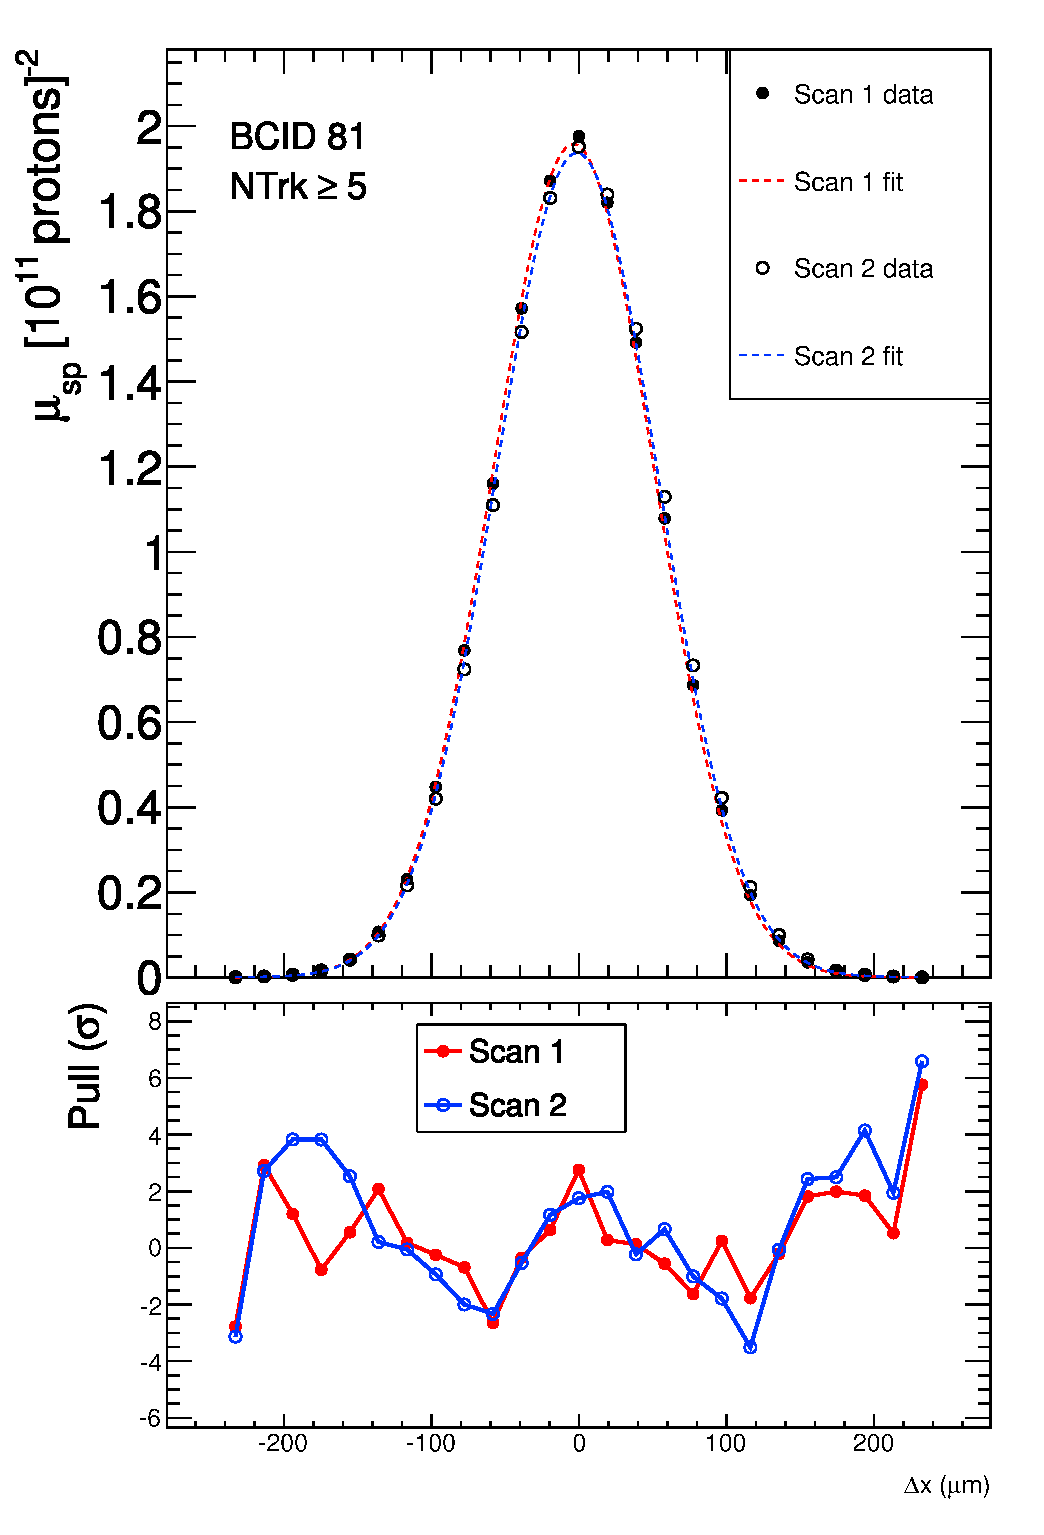
\includegraphics{figures/ch4-reconstruction/c_musp_x_BCID81_NTrkCut5}}
	}
	\subfloat[$y$ scan, BCID 81] {
		\resizebox{3in}{!}{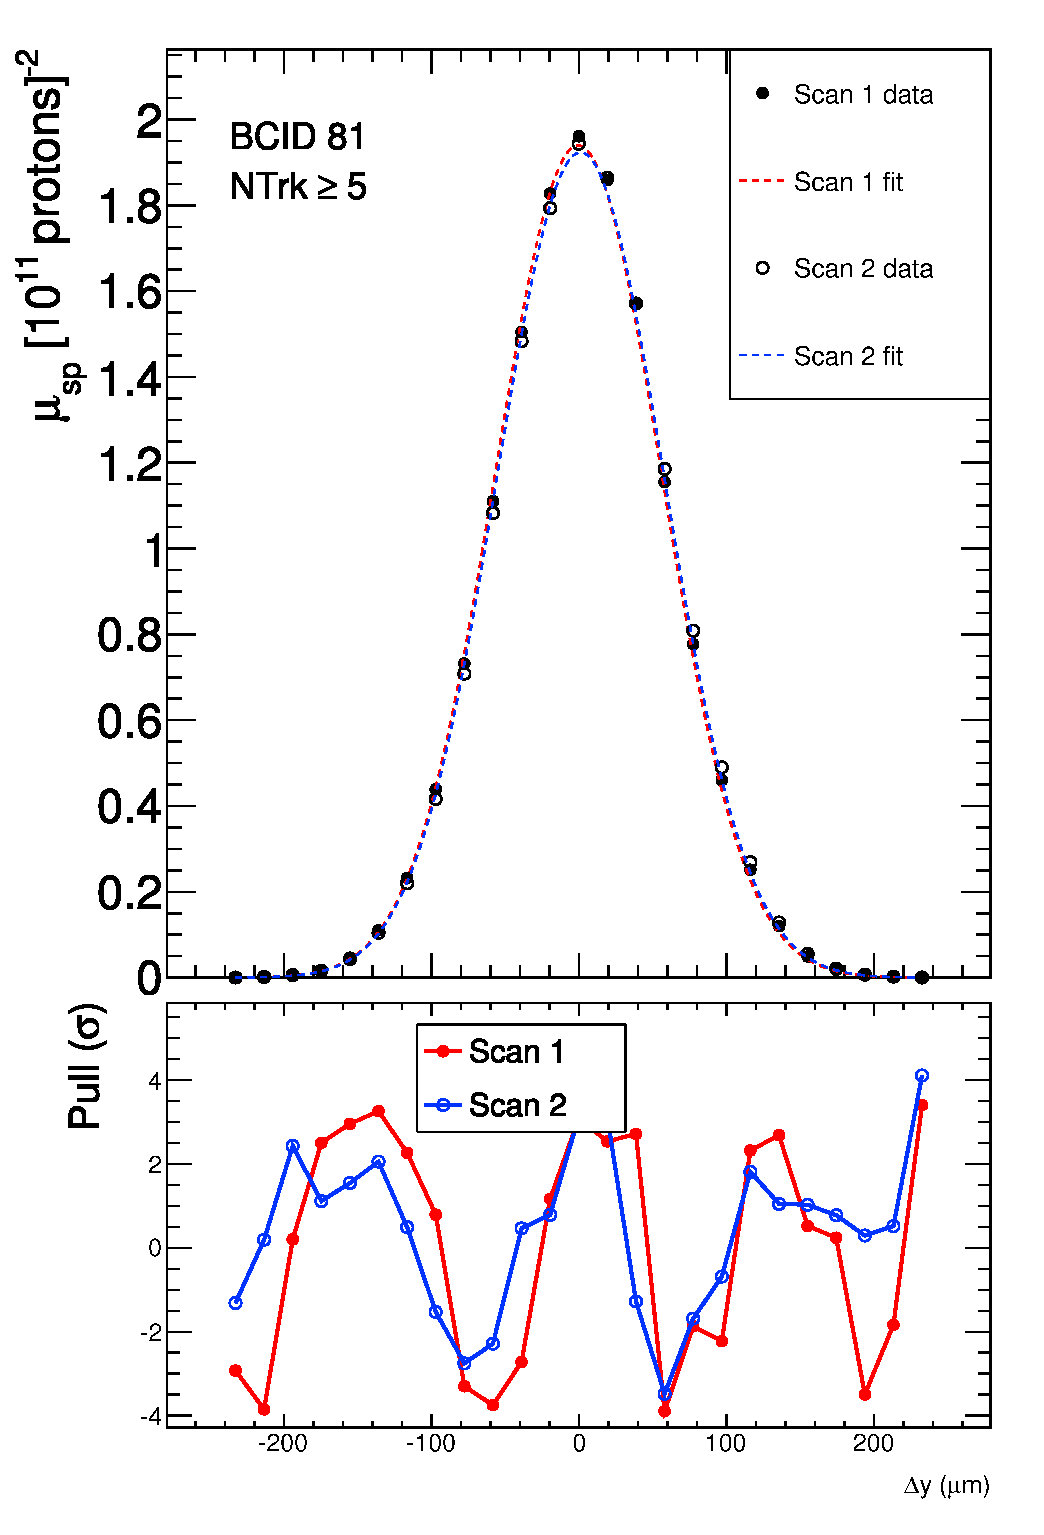
\includegraphics{figures/ch4-reconstruction/c_musp_y_BCID81_NTrkCut5}}
	}\\
	\caption{$\mu_{\textrm{vis}}^{(sp)}$ vs. beam separation, with single gaussian plus constant fits, and pulls.}
	\label{fig:reco-luminosity-vertex-vdm}
\end{figure}

\ 

\textbf{Pileup Scan}

The September 2011 pileup scan is used to derive systematic uncertainties due to the nonlinear response of algorithms with respect to the number of interactions per bunch crossing. The scan was performed at the end of a physics run, displacing the beams in the transverse direction to obtain a sample of data at different pileup values with otherwise identical conditions. The data was triggered by a random trigger selecting events from two bunch crossings, BCIDs 200 and 999. The data are corrected for vertex masking and fakes, with the correction reaching up to 10\% as shown in figure~\ref{reco-luminosity-vertexing-muscan-corrections} with respect to BCM\_VOR. A comparison of the luminosity measurements between vertex counting and BCM\_VOR, shown in figure~\ref{fig:reco-luminosity-vertexing-muscan}, exhibits a slope of about 0.1\% per unit of $\mu$.

\begin{figure}[h]
	\centering
	\subfloat[BCID 200] {
		\resizebox{6.5in}{!}{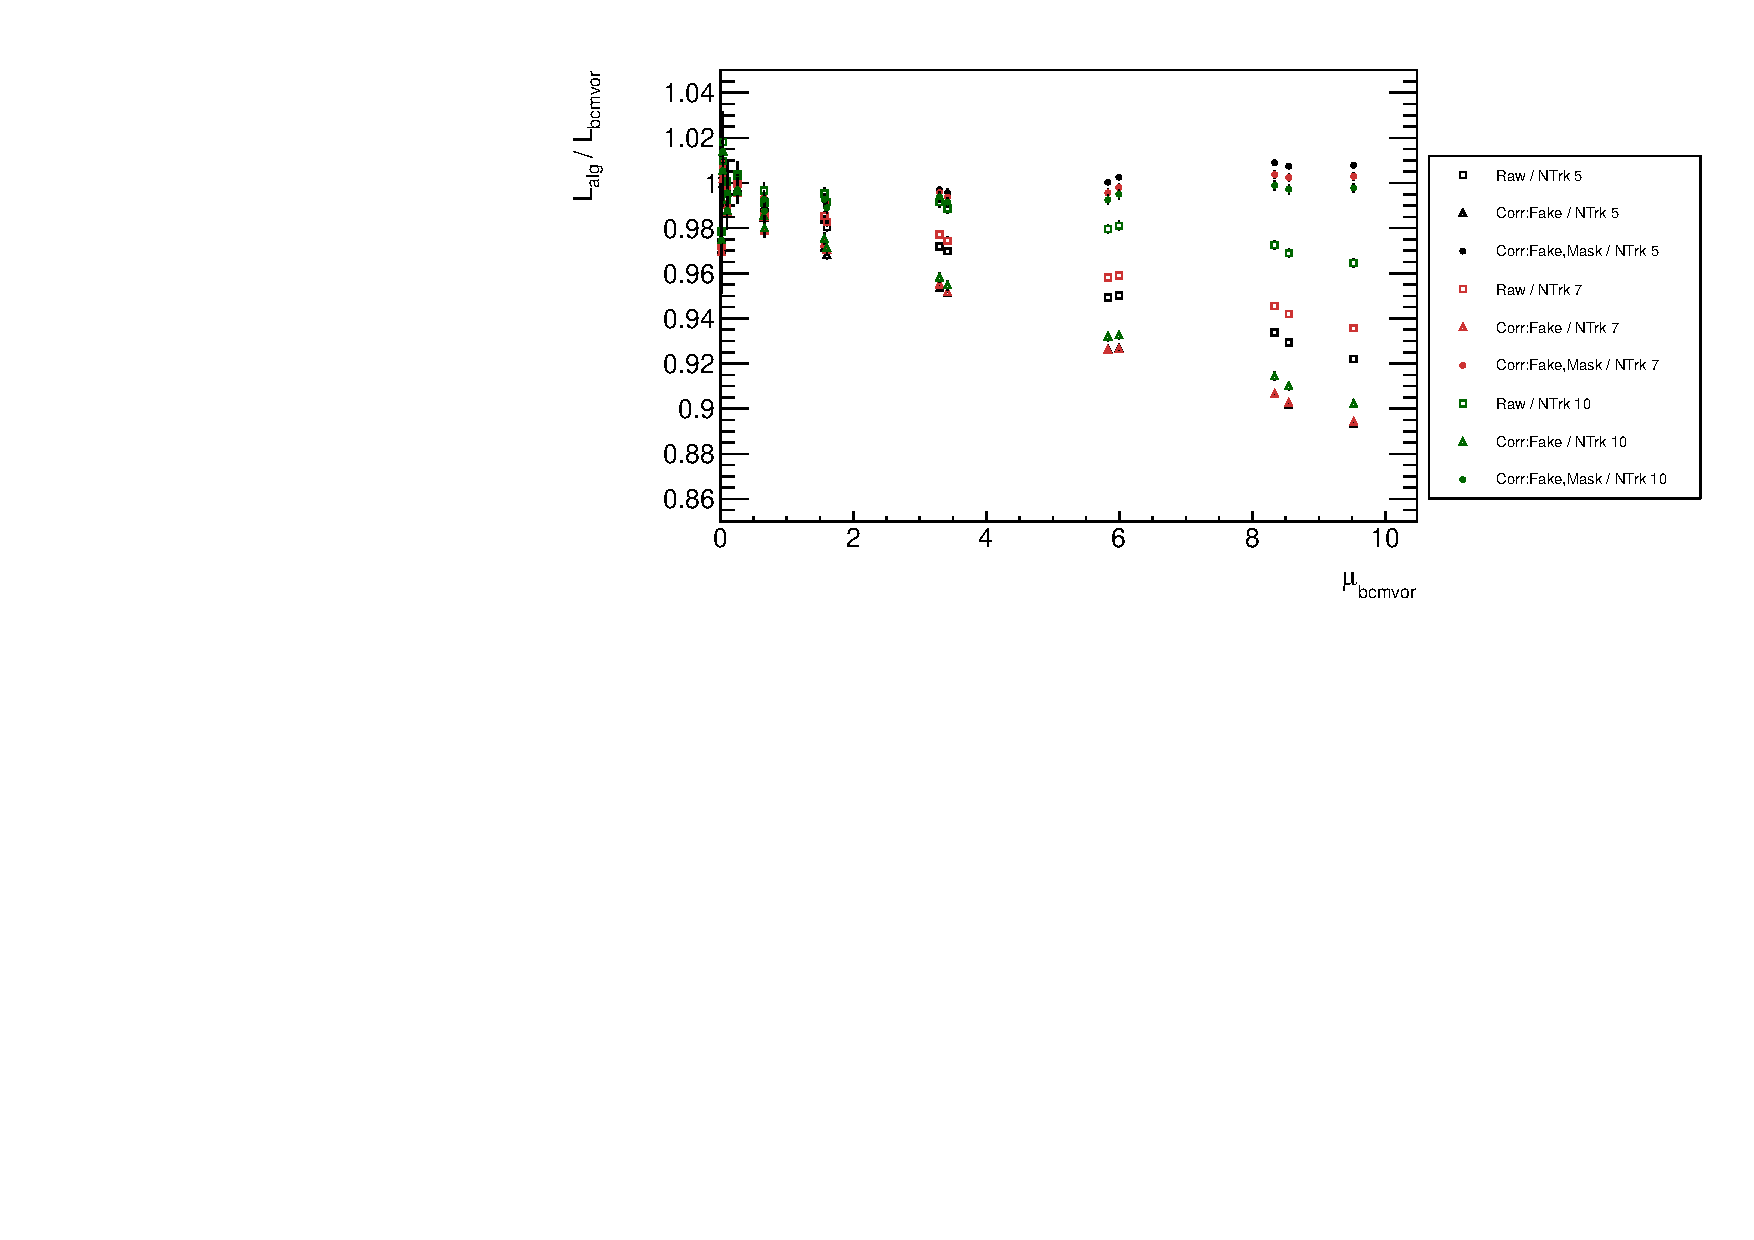
\includegraphics{figures/ch4-reconstruction/c_pileup_corrections_NVtx_BCID200}}
	}\\
	\subfloat[BCID 999] {
		\resizebox{6.5in}{!}{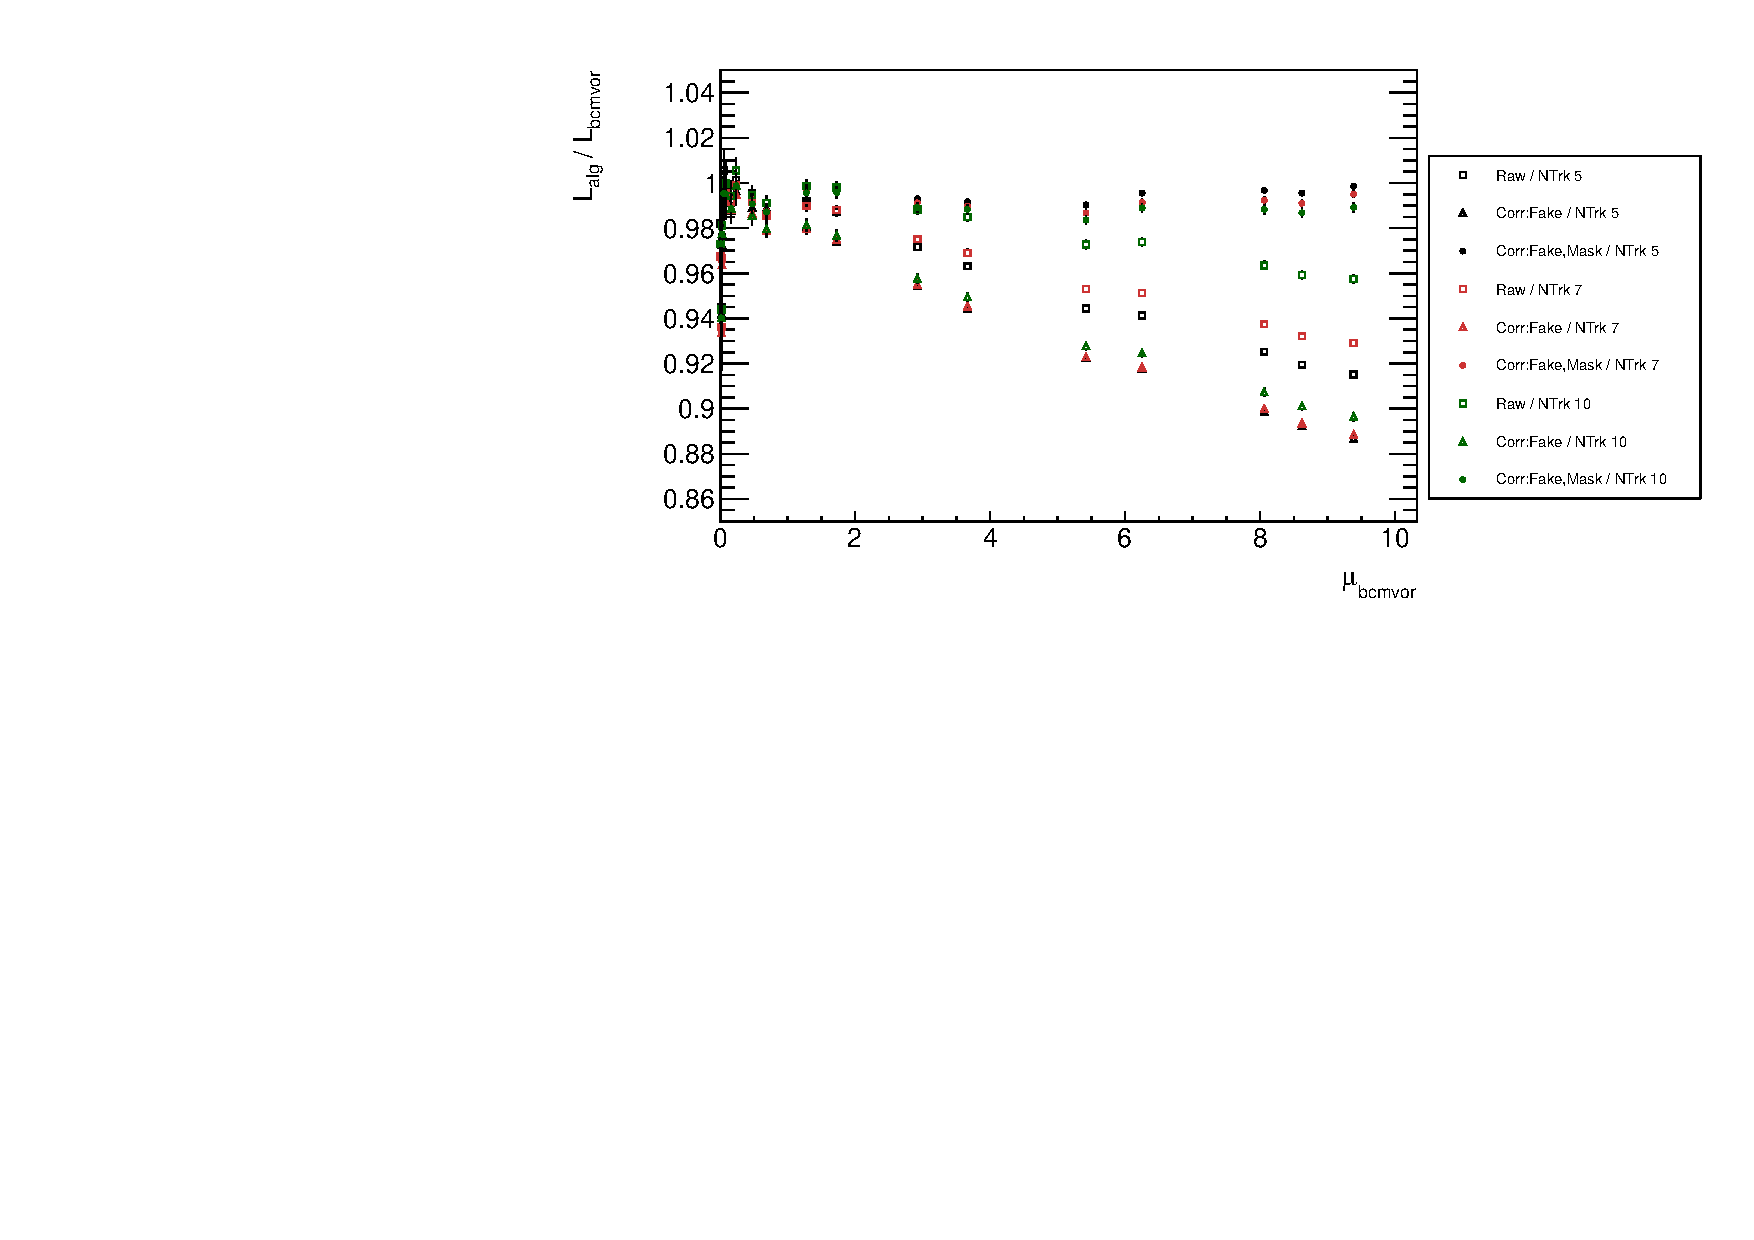
\includegraphics{figures/ch4-reconstruction/c_pileup_corrections_NVtx_BCID999}}
	}
	\caption{Ratio of luminosity values from vertexing and BCM\_VOR, shown with each successive pileup correction applied. Fakes are subtracted first, and masking is corrected second.}
	\label{reco-luminosity-vertexing-muscan-corrections}
\end{figure}

\begin{figure}[h]
	\centering
	\resizebox{6in}{!}{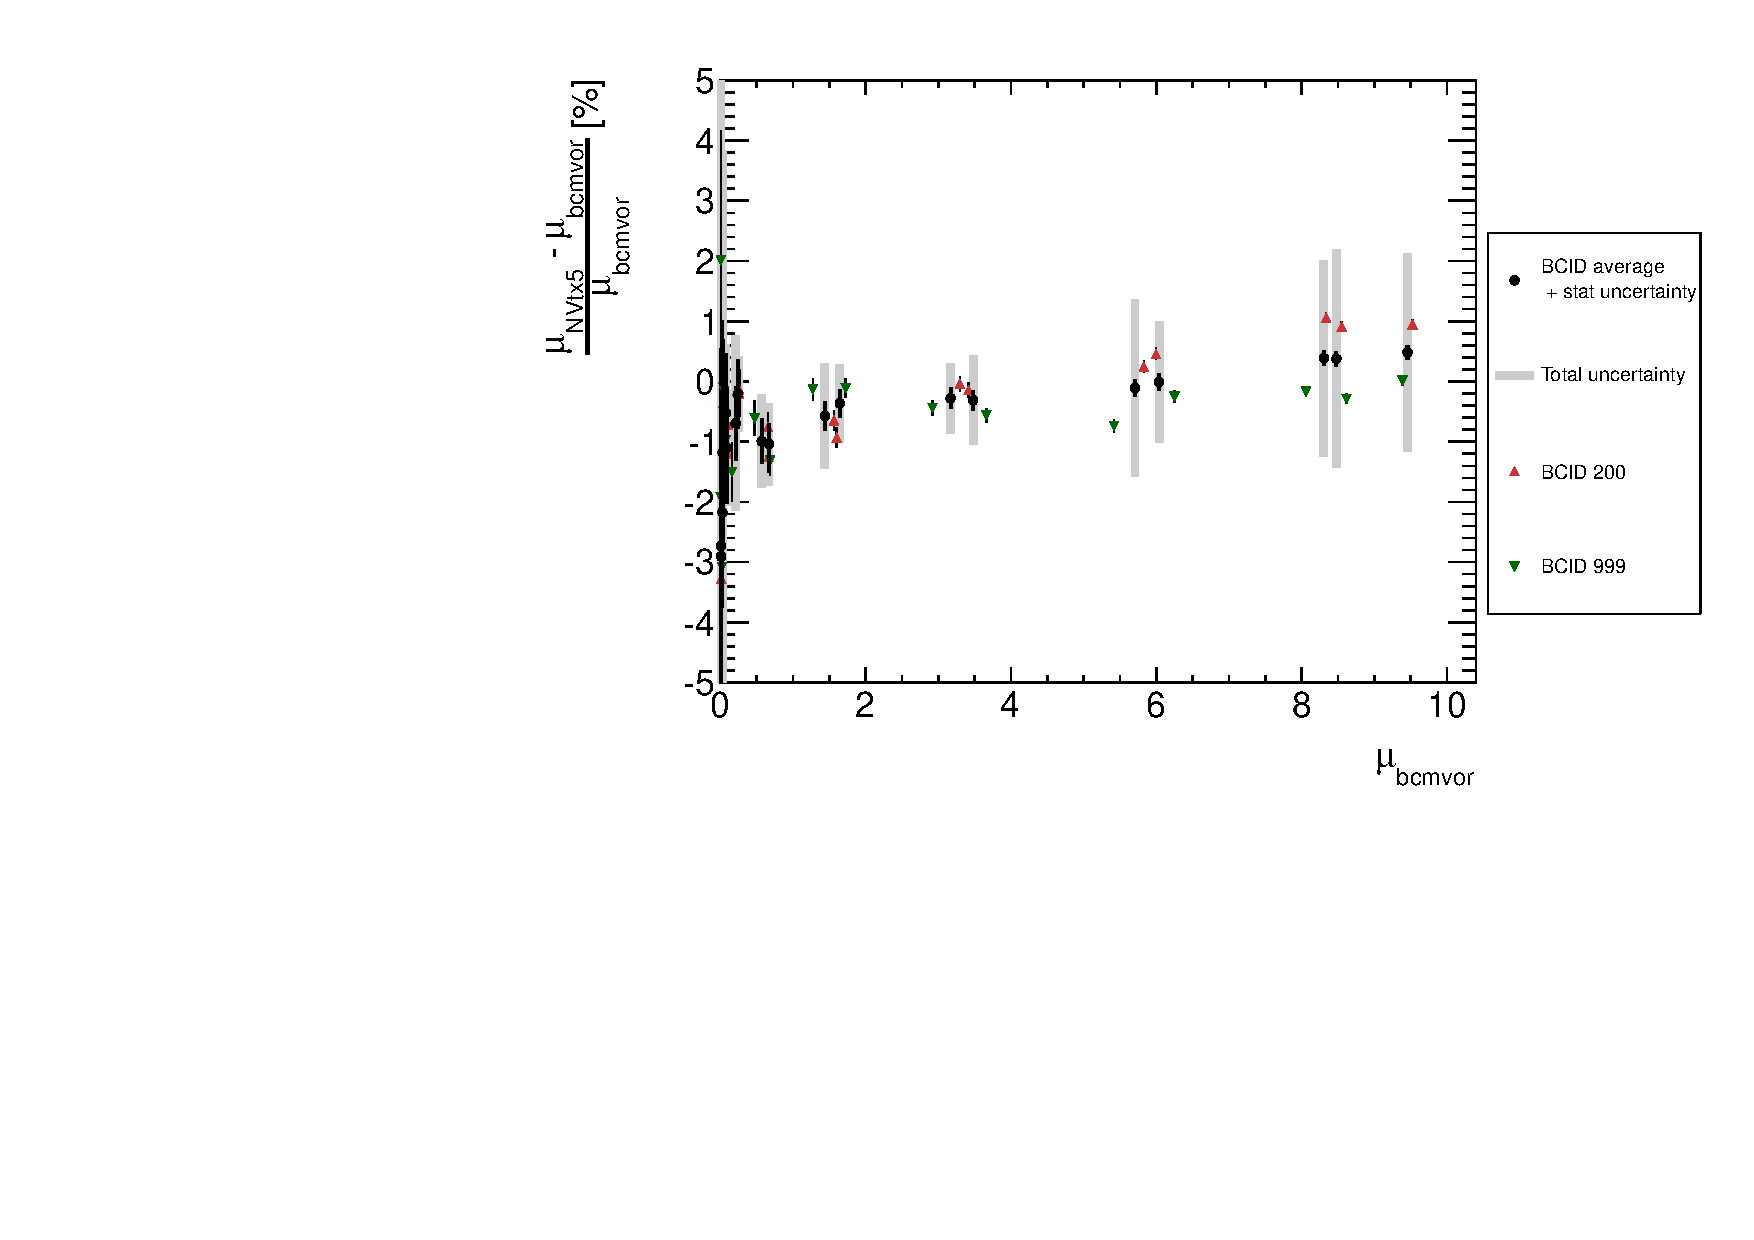
\includegraphics{figures/ch4-reconstruction/c_muscan}}
	\caption{Percent difference between luminosities measured by vertex counting and BCM\_VOR. The central values are taken to be the average between BCIDs 200 and 999.}
	\label{fig:reco-luminosity-vertexing-muscan}
\end{figure}

\ 

\textbf{ALFA Run}

Finally, vertex counting provides a reliable luminosity measurement for the 2011 ALFA run, a special run used for a measurement of the total $pp$ cross section. The beams contain a single colliding bunch pair with $\beta^{*}=90~\mbox{m}$ and $\mu\sim0.03$, in order to measure the scattering angle of elastic $pp$ collisions. A special luminosity analysis is performed to address the very low instantaneous luminosity of $\mathcal{L}\sim5\times 10^{27} \cm^{-2}\mbox{s}^{-1}$, about six orders of magnitude lower than a typical physics fill. The calorimeter methods are unusable due to a lack of sensitivity. For BCM and LUCID, the backgrounds at low instantaneous luminosity have a different composition: afterglow is negligible with a single colliding bunch, but beam-gas interactions can be significant, resulting in an extra 0.2\% systematic uncertainty. The low-pileup conditions are ideal for vertex counting, eliminating the need to perform pileup corrections. The cut on the minimum number of tracks per vertex suppresses the beam-gas backgrounds. The data were recorded by a random trigger at approximately 1~kHz. 

A comparison of luminosity measurements from BCM, LUCID, and vertex counting is shown in figure~\ref{fig:reco-luminosity-alfa}. To be consistent with the primary $pp$ luminosity measurement, the central value is taken from BCM\_VOR; vertex counting shows agreement with this value to within $0.5\%$.

\begin{figure}[h]
	\centering
	\resizebox{5in}{!}{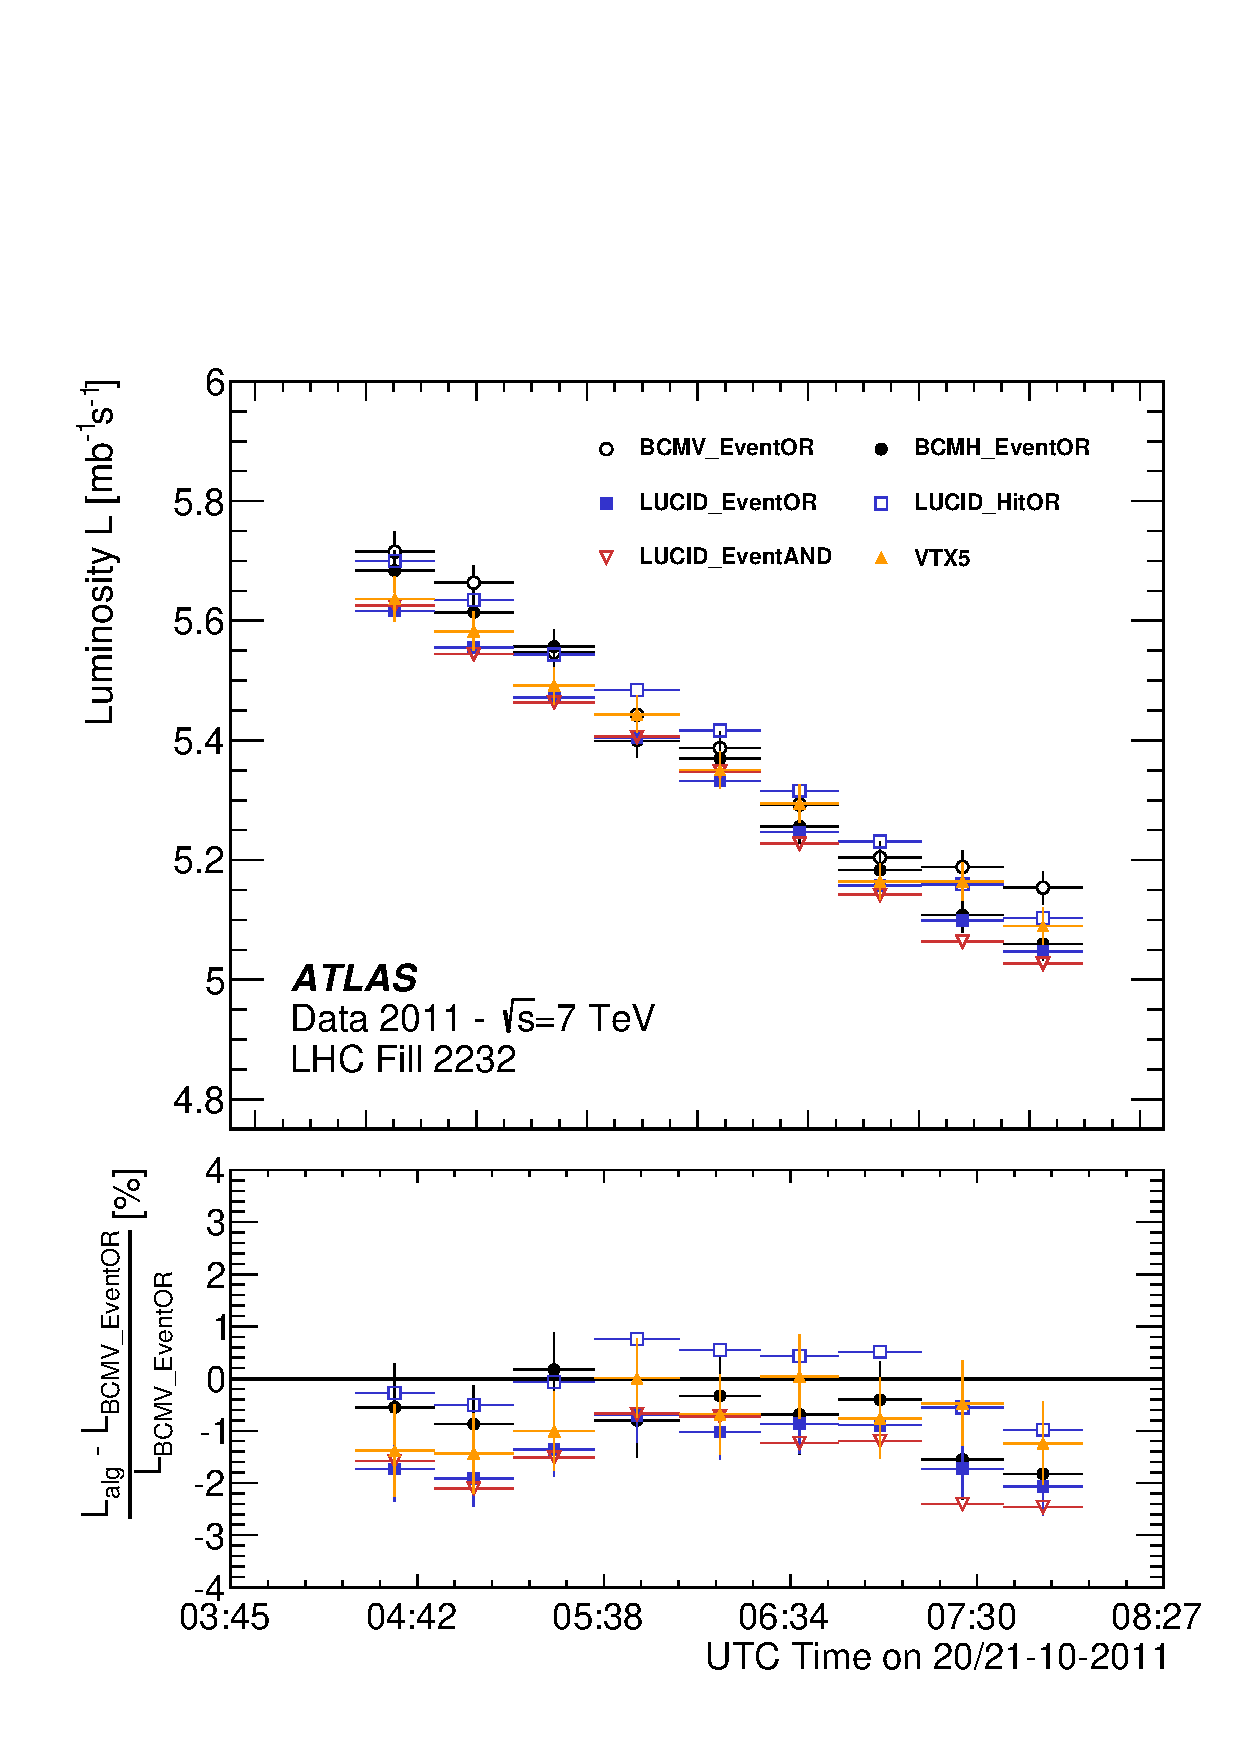
\includegraphics{figures/ch4-reconstruction/c_lumi_combined_191373.pdf}}
	\caption{Luminosities measured by BCM, LUCID, and vertex counting during the $\beta^{*}=90~\mbox{m}$ ALFA run in October 2011.}
	\label{fig:reco-luminosity-alfa}
\end{figure}

\clearpage

\section{Event Reconstruction}\label{sec:event-reconstruction}
Events are reconstructed using a wide variety of algorithms designed to identify the products of collisions at the center of the detector. The algorithms transform the raw data read out from the detector -- hits in the inner detector silicon layers and TRT straws, energy deposits in calorimeter cells, and hits in the muon stations -- into a list of physics objects and their energies or momenta. This section describes the techniques used to identify the objects used in the analyses described in chapters~\ref{ch:model-independent-trilepton-search} and \ref{ch:trilepton-resonance-search}. 


\subsection{Electrons}\label{sec:event-reconstruction-electrons}
The signature of an electron is an energy deposit in the electromagnetic LAr calorimeter and a track reconstructed by the inner detector pointing at the calorimeter energy cluster.  The electron reconstruction algorithm begins by searching for clusters of energy in the calorimeter, based on a grid of $N_{\eta}\times N_{\phi}=200\times256$ towers of size $\Delta\eta\times\Delta\phi = 0.025\times0.025$. The tower energy is the sum of the cell energies in all longitudinal layers within the tower. Energy deposits with $\Et>2.5 \GeV$ within a $3\times 5$ window of towers form the seeds for both electrons and photons.

After passing loose shower shape requirements, the electron reconstruction algorithm searches for a track within a cone of radius $\Delta R=0.3$ around the cluster barycenter. Two hypotheses are used for track pattern recognition and fitting: the standard pion hypothesis, and an electron hypothesis that allows for larger energy losses due to bremsstrahlung. The cluster and track are required to satisfy one of the following two criteria:

\begin{itemize}
	\item The barycenter of the cluster and the track extrapolation to the middle layer of the LAr calorimeter satisfy $\Delta\phi<0.2$ in the direction of track bending or $\Delta\phi<0.05$ in the other direction. 
	\item The barycenter of the cluster and the track extrapolation to the middle layer of the LAr calorimeter, after rescaling the track momentum to the energy of the cluster, satisfy $\Delta\phi<0.1$ in the direction of track bending or $\Delta\phi<0.05$ in the other direction. 
\end{itemize}
 
For tracks with at least four silicon hits, the track and the cluster must also satisfy $|\Delta\eta|<0.05$. Finally, the cluster and track are rebuilt using algorithms optimized for measurement of the electron properties. The cluster is rebuilt sequentially in all four layers, using an area of $3\times7$ layer-2 cells in the barrel or $5\times5$ layer-2 cells in the end-caps. The tracks of electron candidates are refit using an optimized electron track filter based on the Gaussian Sum Filter (GSF) algorithm~\cite{gsf}. The GSF track and the cluster must satisfy tighter spatial matching criteria: $\Delta\phi<0.1$ in the direction of track bending, or $\Delta\phi<0.05$ in the opposite direction. GSF tracks with less than four silicon hits are required to satisfy even tighter criteria: $|\Delta\eta|<0.35$ or $0.2$ in the TRT barrel or end-cap, and $\Delta\phi<0.03$ in the direction of track bending or $\Delta\phi<0.02$ in the other direction. 

\subsubsection{Identification}
Further requirements can be imposed on electron candidates to suppress backgrounds from sources like misidentified hadronic jets, photon conversions, and electrons from hadron decays. Three increasingly stringent sets of cuts are defined, called loose, medium, and tight\footnote{An alternative method of identification using a likelihood-based multivariate method has been developed, but is not used in this dissertation}. The analyses described in chapters~\ref{ch:model-independent} and \ref{ch:resonance} use the tight cuts to select signal electrons, and the medium and loose cuts to derive data-driven background estimates. The loose set of cuts impose requirements on the shower shape in the first and second calorimeter layers, the quality of the track, the fraction of energy in hadronic calorimeter cells behind the LAr cells, and the spatial match of the track and the calorimeter cluster. The medium set of cuts consist of more stringent versions of the loose cuts, and additionally require a small track impact parameter with respect to the primary vertex, a minimum number of high-threshold TRT hits associated with the track, and a hit in the innermost pixel layer. The tight set of cuts again consist of more stringent versions of the medium cuts, with an additional cut on the ratio of the cluster energy to the track momentum ($E/p$) and a veto of candidates associated to a photon conversion vertex. 

\textcolor{red}{Consider putting a table in instead of a block of text.}

\subsubsection{Efficiency Measurements}\label{sec:reco-electron-efficiency}
The efficiency to detect an electron can be factorized into several components. The efficiency to detect a cluster in the electromagnetic calorimeter is very high, above $99\%$ for electrons with $\Et=15 \GeV$ and $99.9\%$ for $\Et=45 \GeV$. The reconstruction efficiency, covering the matching of a good-quality track to the cluster, and the identification efficiencies, covering the identification cuts with respect to reconstructed electrons, are measured using tag-and-probe techniques targeting $Z\rightarrow ee$ and $J/\Psi\rightarrow ee$ events~\cite{TheATLASCollaboration:2014vz}. One electron, the tag, is required to satisfy strict selection criteria, while the second electron, the probe, is used for efficiency measurements. The combined reconstruction and identification efficiencies are shown in figure~\ref{fig:electron-id-efficiencies}. The reconstruction efficiency makes up $1-5\%$ of the efficiency loss for electrons with $\Et<20 \GeV$, and less than $1\%$ for electrons with $\Et>80 \GeV$. The efficiencies are computed for both data and simulation, and the ratio between the two is used to correct the efficiency in simulation.

\begin{figure}[htbp]
	\centering
	\subfloat[] {
		\resizebox{0.45\textwidth}{!}{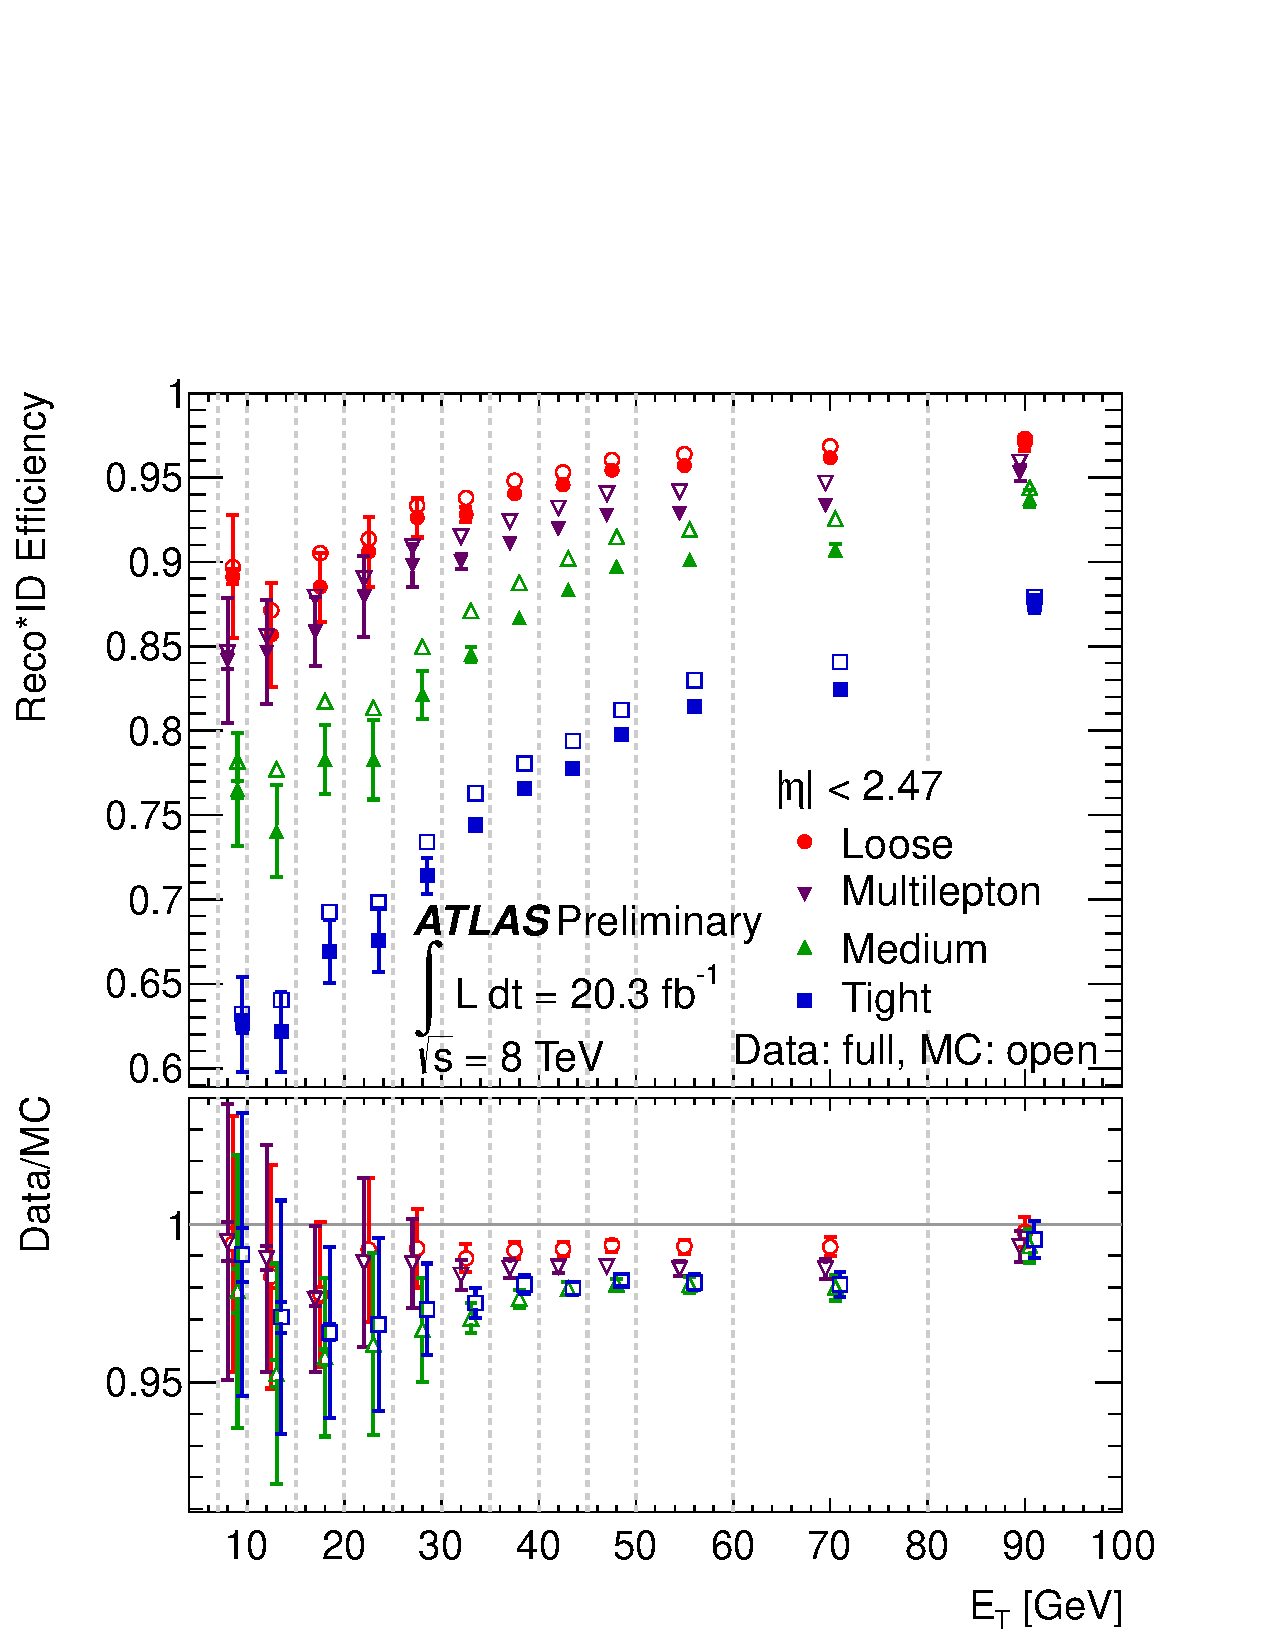
\includegraphics{figures/ch4-reconstruction/el_eff_idplusreco_ET}}
	}
	\hfill
	\subfloat[] {
		\resizebox{0.45\textwidth}{!}{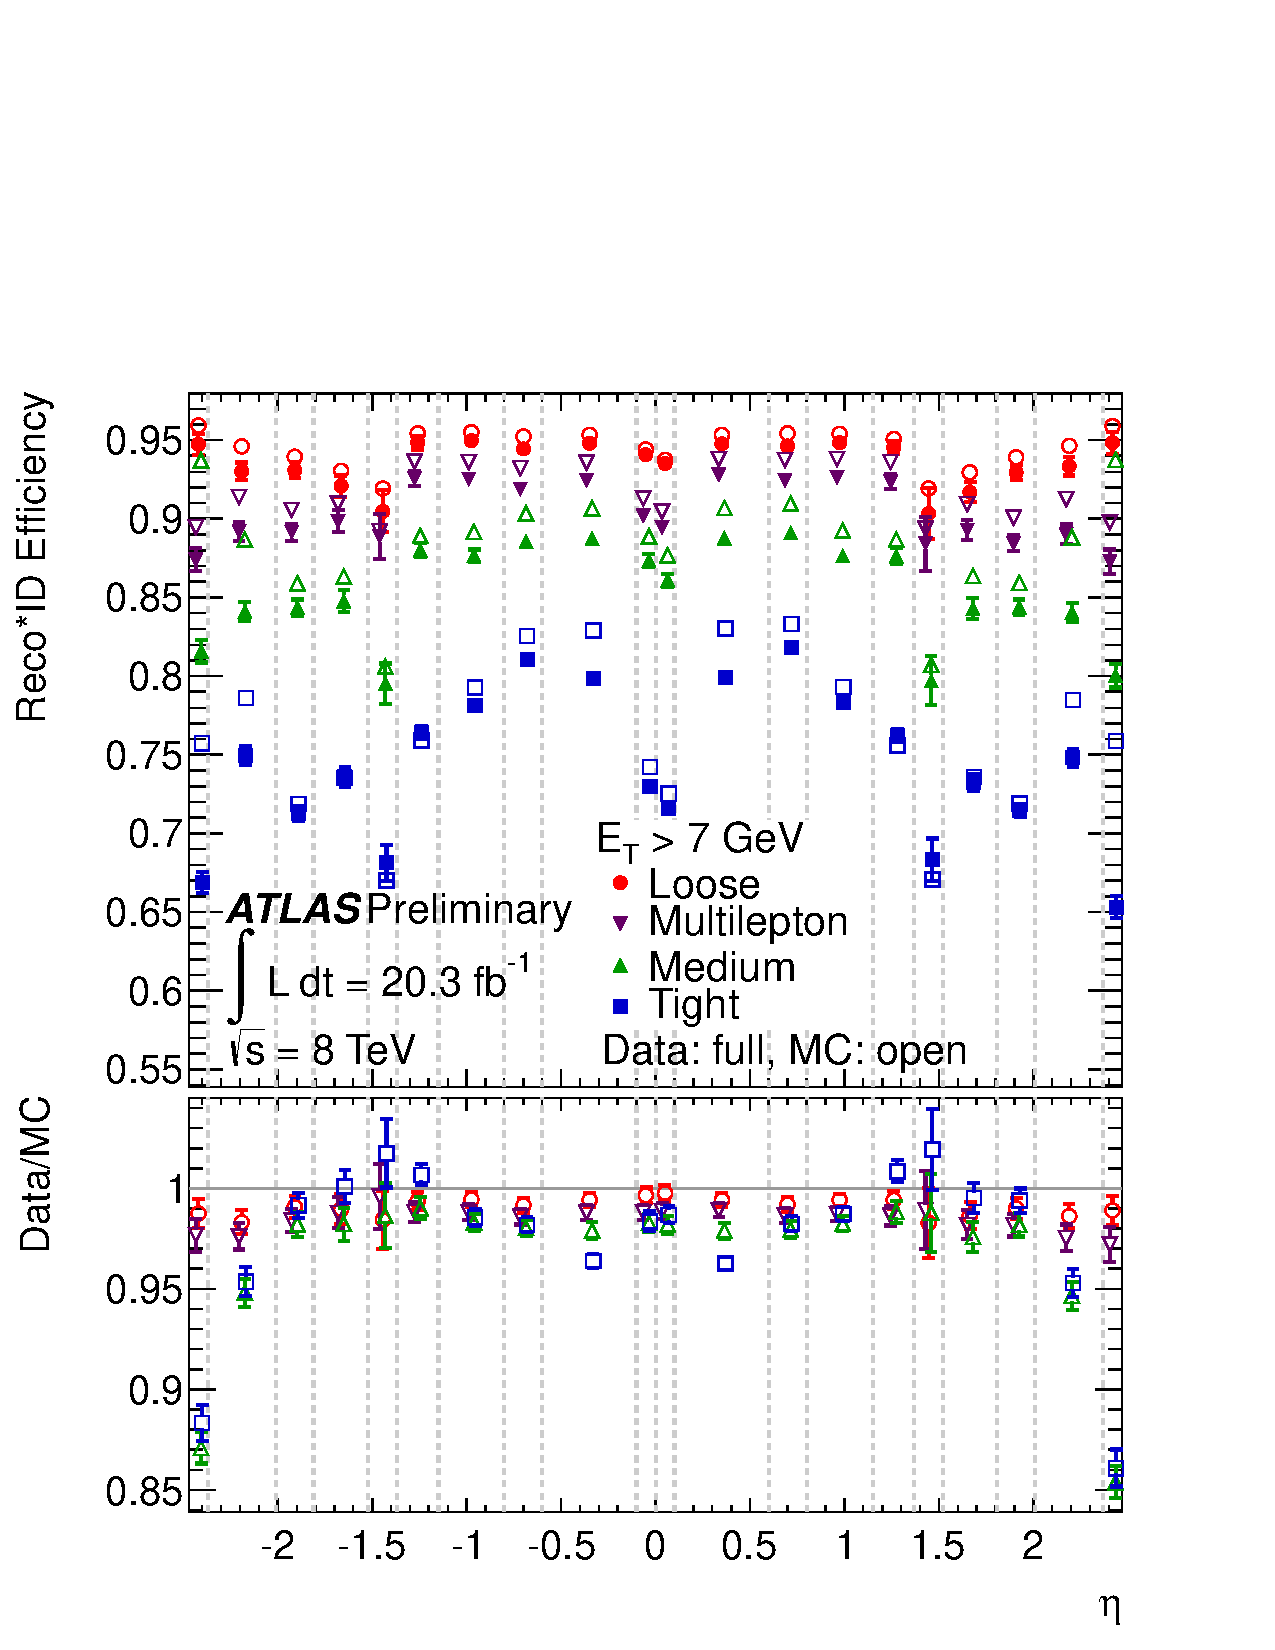
\includegraphics{figures/ch4-reconstruction/el_eff_idplusreco_eta}}
	}
	\caption{The combined reconstruction and identification efficiencies with respect to electrons detected as a cluster in the electromagnetic calorimeter, shown as a function of $\Et$ (left) and $\eta$ (right).}
	\label{fig:electron-id-efficiencies}
\end{figure}


\subsubsection{Energy and Momentum Measurement}\label{sec:reco-electron-energymomentum}
For electron candidates with at least four silicon hits, the energy of the electron is taken from the calorimeter measurement, while the trajectory is taken from the GSF track. Candidates with fewer silicon hits are not used in this dissertation. The energy resolution of the calorimeter is parametrized as:

\begin{equation}
	\frac{\sigma(E)}{E} = \frac{a}{\sqrt{e}} \oplus \frac{b}{E} \oplus c,
\end{equation}

where $a$, $b$, and $c$ are the sampling, noise, and constant terms, respectively, and generally vary with $\eta$. The design value of the sampling term is $a\approx 9-10\%$ in the central region, and worsens at higher pseudorapidities due to the increased material in front of the calorimeters. The noise term, due to electronics noise and pileup effects, is approximately $b = 350 \times \cosh\eta \MeV$. The constant term dominates the resolution at high energies, with a design value of $c=0.7\%$. 

As the ATLAS calorimeters are non-compensating, the energy measurement is calibrated using a multivariate algorithm trained on single-electron simulation to determine the most probable electron energy. The method takes into account differences between data and simulation in the energy scales of each longitudinal layer and other detector effects not modeled in simulation. 

After the initial simulation-based calibration, the electron energy scale and resolution are determined using $Z\rightarrow ee$ events. Residual differences in the energy scale between data and simulation are parametrized as:

\begin{equation}
	E^{\mathrm{data}} = E^{\mathrm{simulation}} (1 + \alpha_i),
\end{equation}

where the $\alpha_i$ quantify the energy scale difference in bins of pseudorapidity. The difference in energy resolution is derived assuming that the $Z\rightarrow ee$ invariant mass distribution is well-modeled up to a Gaussian constant term, 

\begin{equation}
	\left(\frac{\sigma_E}{E}\right)^{\mathrm{data}} = \left(\frac{\sigma_E}{E}\right)^{\mathrm{simulation}} \oplus c_i,
\end{equation}

where $i$ again denotes bins in pseudorapidity. Histograms of the $Z\rightarrow ee$ invariant mass distribution in simulation are then produced for a range of $\alpha_i$ and $c_i$ values, and the optimal values are determined using a $\chi^2$ minimization with respect to data. The results are shown in figures~\ref{fig:reco-el-EES} and \ref{fig:reco-el-EER}. 

Sources of systematic uncertainty on the energy scale include the intrinsic accuracy of the $Z\rightarrow ee$ method, determined from closure tests where known scale variations are injected into simulation, calorimeter gain and pedestal dependence, data-simulation differences in the calibration of the calorimeter layers, and the modeling of material in front of and within the calorimeter. The total uncertainty ranges from $0.03$-$0.22$\% for $\Et=40 \GeV$ and $0.27$-$2.25$\% for $\Et = 200 \GeV$, with larger uncertainties in the pseudorapidity range $1.37<|\eta|<1.82$ corresponding to the transition region between the barrel and the end-cap. 

The systematic uncertainty on the energy resolution less than $10\%$ for electrons with $\Et<50 \GeV$, and asymptotically approaches $\sim 40\%$ for high $\Et$. At low energies, the pileup contribution to the noise term, $b$, dominates the uncertainty; at higher energy, uncertainty is due to a mix of the sampling term, $a$, the pileup contribution to $b$, the modeling of material, and the intrinsic accuracy of the $Z\rightarrow ee$ method.


\subsection{Muons}\label{sec:event-reconstruction-muons}
Muons are identified by matching tracks in the muon spectrometer to tracks in the inner detector. The requirements differ based on the instrumentation available in the vicinity of the muon candidate. The analyses described here use \emph{combined} muons, consisting of tracks reconstructed independently in the inner detector and the muon spectrometer. The muon momentum is determined from a statistical combination of the two track's parameters and their corresponding covariance matrices. Combined muons have the highest purity, but suffer from a loss of acceptance near $\eta\sim 0$, where the muon spectrometer has gaps to accommodate services for the inner detector and calorimeters, and $1.1<\eta<1.3$, where some trajectories only pass through one muon station due to incomplete installation. The remaining categories are \emph{standalone} (SA) muons, consisting of a track ony in the muon spectrometer; \emph{segment-tagged} (ST) muons, consisting of an inner detector track and one or more track segments in the MDT or CSC chambers; and \emph{calorimeter-tagged} (CaloTag) muons, consisting of an inner detector track matched to a calorimeter energy deposit consistent with the passage of a muon. These categories recover efficiency in regions of the detector with less instrumentation at the cost of lower muon purity, and are not used in this dissertation. 

For all categories of muons, the inner detector track is required to have at least 1 pixel hit, at least 5 SCT hits, at most 2 pixel or SCT holes, and at least 9 TRT hits for $0.1<|\eta|<1.9$. Energy losses in the calorimeter due to ionization, bremsstrahlung, and electron pair production must also be taken into account. 

\subsubsection{Efficiency}\label{sec:reco-muon-efficiency}
The efficiency of the reconstructing CB muons is measured as:

\begin{equation}
	\epsilon(\mathrm{CB}) = \epsilon(\mathrm{CB}|\mathrm{ID}) \epsilon(\mathrm{ID}|\mathrm{MS}),
\end{equation}

where $\epsilon(\mathrm{CB}|\mathrm{ID})$ is the probability that a muon reconstructed as an inner detector track is also reconstructed as a CB muon, and $\epsilon(\mathrm{ID}|\mathrm{MS})\approx \epsilon(\mathrm{ID})$ is the probability that a muon with a track in the muon spectrometer, i.e. a CB or SA muon, is also reconstructed as an inner detector track. The latter approximation is made because $\epsilon(\mathrm{ID})$ is not directly accessible in data. 

The efficiencies are measured using tag-and-probe techniques similar to those described in section~\ref{sec:reco-electron-efficiency}, targeting $Z\rightarrow\mu\mu$ and $J/\Psi\rightarrow\mu\mu$ events. In this case, the tag muon is required to be a CB muon, and the probe muon is a CB or SA muon in the case of measuring $\epsilon(\mathrm{ID}|\mathrm{MS})$, and a CaloTag muon for the measurement of $\epsilon(\mathrm{CB}|\mathrm{ID})$. The efficiencies for all types of muon are shown in figure~\ref{fig:reco-muon-efficiency}. CB muons have an efficiency of greater than $97\%$ in most of the pseudorapidity range, except for significant inefficiencies due to gaps in the muon spectrometer in the ranges $|\eta|<0.1$ and $1.1<\eta<1.3$. The measured efficiencies in data and simulation agree to within $\sim2\%$, and the ratios in each pseudorapidity bin are used as scale factors to correct the efficiency in simulation. The systematic uncertainty on the scale factors is in the range $0.1$-$0.3\%$, rising near $|\eta|\sim 0$ and $|\eta|\sim 2.5$.

\begin{figure}[htbp]
	\centering
	Figure 3 from muon paper, and 5a
	\caption{Top: Muon reconstruction efficiencies as a function of $\eta$ for muons with $\pt>10 \GeV$. The uncertainty bars on the points indicate statistical uncertainties. Bottom: The ratio between the measured and simulated efficiencies, with the combination of statistical and systematic uncertainties indicated by the uncertainty bars.}
	\label{fig:reco-muon-efficiency}
\end{figure}


\subsubsection{Energy Scale and Resolution}
The muon momenta in simulation are scaled and smeared to match the momentum scale and resolution in data. The corrections are derived in bins of $\eta$ and $\phi$, with boundaries chosen to minimize the variation of the correction in each bin, and are applied separately to the transverse momenta measured by the inner detector (ID) and the muon spectrometer (MS). Specifically, the correction is implemented as:

\begin{equation}
	\pt^{\mathrm{Cor,Det}} = \frac{\pt^{\mathrm{MC,Det}} + \sum_{n=0}^1 s_n^{\mathrm{Det}(\eta,\phi)(\pt^{\mathrm{MC,Det}})^n}}{1+\sum_{m=0}^2 \Delta r_m^{\mathrm{Det}}(\eta,\phi)(\pt^{\mathrm{MC,Det}})^{m-1}g_m},
\end{equation}

where Det=ID or MS, the $\Delta r_m^{\mathrm{Det}}(\eta,\phi)$ parametrize the momentum resolution smearing, the $s_n^{\mathrm{Det}}(\eta,\phi)$ parametrize the scale corrections, and the $g_m$ are normally-distributed random variable with mean 0 and width 1\footnote{Note that this equation does not apply to cases where the resolution is data is better than that in simulation. In these cases, the resolution difference is included in the positive ID and MS variations, and the effect of the positive variation on the physical observables is symmetrized about the nominal value.}. The constant scale correction term, $s_0^{\mathrm{MS}}$, accounts for the difference between data and simulation in the energy lost by muons before reaching the muon spectrometer. $s_0^{\mathrm{ID}}$ is set to zero due to the negligible energy loss before the inner detector. The linear terms, $s_1^{\mathrm{ID,MS}}$, models discrepancies between data and simulation in the magnetic field integral and the radial dimension of the detector. The resolution corrections $\Delta r_m^{\mathrm{Det}}$ represent deviations from the resolution in data, which is parametrized empirically as:

\begin{equation}
	\frac{\sigma(\pt)}{\pt} = \frac{r_0}{\pt} \oplus r_1 \plus r2\cdot\pt,
\end{equation}

where the $r_0$ term describes energy lost by muons as they traverse the material of the detector, the $r_1$ term describes multiple scattering, magnetic field inhomogeneities, and local radial displacements, and the $r_2$ term describes intrinsic resolution effects due to the spatial resolution of the hit measurements and residual misalignment. 

The corrections are derived from $J/\Psi\rightarrow\mu\mu$, $\Upsilon\rightarrow\mu\mu$, and $Z\rightarrow\mu\mu$ events using a template maximum likelihood fit, similar to that described in section~\ref{sec:reco-electron-energymomentum}. The effect of the corrections on the invariant mass distribution of $Z\rightarrow\mu\mu$ events is shown in figure~\ref{fig:reco-muon-momentum-corrections}, along with the total systematic uncertainty. \textcolor{red}{Consider showing the muon momentum resolution, figure 14.}

\begin{figure}
	Figure 10c
	\label{fig:reco-muon-momentum-corrections}
\end{figure}



\subsection{Tau Leptons}\label{sec:event-reconstruction-taus}
The signature of tau leptons is significantly more complex than electrons and muons due to the fact that they decay to a diverse set of final states. 


\subsubsection{Efficiency}

\subsubsection{Energy Scale and Resolution}



\subsection{Jets}\label{sec:event-reconstruction-jets}

%\subsubsection{Efficiency}

\subsubsection{Energy Scale and Resolution}

\subsubsection{$B$-tagging}\label{sec:event-reconstruction-bjets}

\subsection{Invisible Particles}\label{sec:event-reconstruction-met}

\chapter{Model Independent Trilepton Search}\label{ch:model-independent-trilepton-search}

Events containing three or more leptons are useful probes of phenomena beyond the Standard Model. On one hand, the expected Standard Model backgrounds are typically small; depending on the kinematic requirements on the three leptons, such events arise dominantly from diboson production ($WZ$, $ZZ$), or from event where one or more leptons arises from misidentified or semileptonically decaying jets. On the other hand, the production of three or more leptons is predicted by many models of phenomena beyond the Standard Model, as described in section~\ref{sec:beyond-the-standard-model}. This dissertation presents two such searches: a model-independent search for non-resonant production of three or more leptons in many signal regions, and a signature-driven search for resonance trilepton production in the context of heavy leptons. 

This chapter presents a search for physics beyond the Standard Model using events containing three or more leptons. The search uses $20.3~\ifb$ of $pp$ collision data taken at $\sqrt{s}=8~\mbox{TeV}$ with the ATLAS detector. Many signal regions are defined based on the properties of the leptons, jets, and overall momentum imbalance of the event, with the goal of being broadly sensitive to the non-resonant production of trilepton final states by phenomena beyond the Standard Model. 

\section{Event Selection}\label{sec:model-independent-event-selection}

This section describes the selection of events containing at least three leptons in both $pp$ collision data and in the Monte Carlo simulation samples. 


\subsection{Object Definitions}\label{sec:model-independent-object-definitions}

\subsubsection{Leptons}\label{sec:model-independent-lepton-definitions}

The analysis requires at least three reconstructed electrons, muons, or hadronically decaying tau leptons, as described in section~\ref{sec:object-reconstruction}. A summary of the lepton selections is shown in table~\ref{table:lepton-selections}. Leptons are required to satisfy the following requirements:

\begin{itemize}

	\item \underline{\textbf{Transverse momentum}}: Electrons and muons must have $\pt>15 \GeV$, while hadronically decaying tau leptons must have $\pt>20 \GeV$. The transverse momentum cut is driven by the availability of triggers with which to perform the data-driven reducible background estimate, described in section~\label{sec:fake-factors}. 

	\item \underline{\textbf{Geometrical acceptance}}: Electrons are required to have $|\eta|<2.47$, excluding the transition region $1.37<|\eta|<1.52$ between the barrel and end-cap calorimeters. Muons and tau leptons are required to have $|\eta|<2.5$.

	\item \underline{\textbf{Particle identification}}: To suppress the reducible backgrounds, the leptons must satisfy strict requirements related to particle identification, as described in section~\ref{sec:object-reconstruction}. Electrons candidates must satisfy the tight++ set of identification cuts. Electrons are neglected if they fall in a region affected by the presence of a dead front end board in the first or second sampling layer, a dead high voltage supply, or a masked cell in the core. Muons are required to be \emph{combined}, with associated hits in the inner detector and muon spectrometer. Specifically, 
	\begin{itemize}
	  \item A B-layer hit (if expected).
	  \item $\geq1$ pixel hit and $\geq5$ SCT hits, including any dead sensors along the trajectory.
	  \item $<3$ total holes in the pixel and SCT. 
	  \item \textcolor{red}{Needs more explanation} If $0.1 < |\eta| < 1.9$, require $n_{\mathrm{TRT}}^{\mathrm{hits}}+n_{\mathrm{TRT}}^{\mathrm{outliers}} > 5$ and $n_{\mathrm{TRT}}^{\mathrm{outliers}} < 0.9 \times (n_{\mathrm{TRT}}^{\mathrm{hits}}+n_{\mathrm{TRT}}^{\mathrm{outliers}})$,
	 % \item Else if $|\eta| < 0.1$ or $|\eta| > 1.9$ and $n_{\mathrm{TRT}}^{\mathrm{hits}}+n_{\mathrm{TRT}}^{\mathrm{outliers}} > 5$, then require $n_{\mathrm{TRT}}^{\mathrm{outliers}} < 0.9 \times (n_{\mathrm{TRT}}^{\mathrm{hits}}+n_{\mathrm{TRT}}^{\mathrm{outliers}})$.
	\end{itemize}

	Finally, tau leptons must satisfy the \texttt{ BDT-tight} selection criteria.

	\item \underline{\textbf{Impact parameter}}: The inner detector track associated with electrons and muons must be consistent with originating from the event primary vertex. The transverse impact parameter significance, defined as the transverse impact parameter $d_0$ divided by its uncertainty $\sigma_{d_0}$, is required to satisfy $\frac{d_0}{\sigma_{d_0}}<3$. Similarly, the longitudinal impact parameter $z_0$ is required to satisfy $z_0\sin\theta < 0.5~\mm$. These requirements suppress leptons from semileptonic heavy flavor decays. 

	\item \underline{\textbf{Isolation}}: To further reduce the impact of non-prompt and misidentified leptons, the leptons are required to be isolated from other activity in the event. The cuts on electrons and muons are similar, and limit the amount of nearby activity as measured by inner detector tracks and calorimeter energy deposits:

	\begin{itemize}
		\item For both electrons and muons, a cut is applied on \verb.ptcone30., the sum of transverse momenta of tracks associated to the same primary vertex as the lepton within a cone of $\Delta R<0.3$. 
		\item For muons, a cut is applied on \verb.Etcone30., the scalar sum of transverse energies of calorimeter cells within $\Delta R<3.0$ of the muon track. 
		\item For electrons, a cut is applied on \verb.TopoEtcone30., the sum of topological calorimeter clusters within a cone of $\Delta R < 3.0$. The use of topological clusters reduces the impact of pileup and out-of-cone leakage. 
	\end{itemize}

	All isolation variables are required to be less than $10\%$ of the lepton transverse momentum for leptons with $\pt<100~\mbox{GeV}$, and less than $10~\mbox{GeV}+0.01\times \pt$ for leptons with $\pt\geq 100~\mbox{GeV}$. 
\end{itemize}

\begin{table}[h]
	\footnotesize
		\begin{tabular}{ccc}
			Cut & Electrons & Muons \\
			\hline
			Object ID & Tight++ & Combined Tight \\
			Leading (trigger) $\ET/\pt$ & $\ET>26~\mbox{GeV}$ & $\pt>26~\mbox{GeV}$ \\
			Subleading $\ET/\pt$ & $\ET>15~\mbox{GeV}$ & $\pt>15~\mbox{GeV}$ \\
			Trigger Acceptance & $(|\eta|<2.47)\ \&\&\ !(1.37<|\eta|<1.52)$ & $|\eta|<2.4$ \\
			Acceptance & $(|\eta|<2.47)\ \&\&\ !(1.37<|\eta|<1.52)$ & $|\eta|<2.5$ \\
			Calo. Isolation & \verb.TopoEtcone30. $<\left\{\begin{array}{ccl} 0.1\times \ET & : & \ET < 100~\mbox{GeV} \\ 10~\mbox{GeV}+0.01\times \ET & : & \ET>100~\mbox{GeV} \end{array}\right.$ & \verb.Etcone30. $<\left\{\begin{array}{ccl} 0.1\times \pt & : & \pt < 100~\mbox{GeV} \\ 10~\mbox{GeV}+0.01\times \pt & : & \pt>100~\mbox{GeV} \end{array}\right.$ \\
			Track Isolation & \verb.ptcone30. $<\left\{\begin{array}{ccl} 0.1\times \ET & : & \ET < 100~\mbox{GeV} \\ 10~\mbox{GeV}+0.01\times \ET & : & \ET>100~\mbox{GeV} \end{array}\right.$ & \verb.ptcone30. $<\left\{\begin{array}{ccl} 0.1\times \pt & : & \pt < 100~\mbox{GeV} \\ 10~\mbox{GeV}+0.01\times \pt & : & \pt>100~\mbox{GeV} \end{array}\right.$ \\
			Track $d_0$ & $\frac{d_0}{\sigma_{d_0}}<3$  \\
			Track $z_0$ & $z_0\sin\theta<0.5~\mbox{mm}$  \\
		\end{tabular}
	\caption{Detailed list of lepton selections.}
	\label{table:lepton-selections}
\end{table}

\subsubsection{Jets and Missing Transverse Energy}\label{sec:model-independent-jets-met}

Jets are reconstructed from topological clusters using the \antikt\ jet algorithm~\cite{Cacciari:2008gp} with a distance parameter of $R = 0.4$ and full four-momentum recombination and are calibrated with a local cluster weighting (LCW) algorithm ({AntiKt4LCTopoJets})~\cite{ATLAS-CONF-2010-053}. The LCW algorithm determines if a topological cluster in the calorimeter is of hadronic or electromagnetic origin, and applies the appropriate energy correction. The jet response also depends on pileup conditions; this is accounted for using the jet area subtraction method provided by the JetEtMiss group~\cite{JetEtmissRecommendations2012}.

Jets are required to have $\pt>30~\mbox{GeV}$, in order to limit the presence of pileup jets. For the geometrical acceptance, jets must lie in the range $|\eta|<4.5$, so that the jet falls within instrumented regions of the detector. Pileup jets are additionally suppressed with a cut on the jet vertex fraction: the $\sum \pt$ of tracks within the jet cone and associated with the selected primary vertex must be at least $50\%$ of the $\sum \pt$ of all tracks within the jet cone~\cite{jvf}. 

Jets consistent with originating from the decay of a $b$-hadron are identified using the MV1 algorithm~\cite{MV1}, with an efficiency of $80\%$. 

The missing transverse momentum, $\Etmiss$, is calculated using the \texttt{ MET\_Egamma10NoTau\_RefFinal} algorithm. Calorimeter cells associated with electrons or photons with $\pt>10 \GeV$ are calibrated specifically to that object; cells associated with tau leptons are not calibrated as tau leptons due to the change in the energy calibration for the objects used in the data-driven reducible background estimate~\ref{sec:fake-factors}. 

\subsection{Triggering}
Collisions events for this analysis are triggered using the unprescaled single-electron or single-muon triggers with the lowest transverse momentum thresholds. At least one of the following triggers must have fired:

\begin{itemize}
	\item \texttt{ EF\_e24vhi\_medium1}: One electron with $\pt>24 \GeV$. The electron must satisfy cuts similar to the medium++ identification criteria at the trigger level, an isolation requirement of $\frac{\pt^{\mathrm{cone}20}}{\pt}<0.1$, and cuts on the leakage into the hadronic calorimeter.
	\item \texttt{ EF\_e60\_medium1}: One electron with $\pt>60 \GeV$. The electron must also satisfy the medium identification cuts, but the isolation and leakage requirements are removed.
	\item \texttt{ EF\_mu24i\_tight}: One muon with $\pt>24 \GeV$, satisfying an isolation requirement of $\frac{\pt^{\mathrm{cone}20}}{\pt}<0.12$.
	\item \texttt{ EF\_mu36\_tight}: One muon with $\pt>36 \GeV$, with the isolation requirement removed.
\end{itemize}

The higher-threshold triggers without isolation requirements recover efficiency at higher $\pt$. Triggered events are required to have an offline lepton matched to the trigger object within $\Delta R=\sqrt{(\Delta\eta)^2+(\Delta\phi)^2} < 0.1$. To avoid trigger turn-on effects near the $\pt$ threshold, the offline lepton must have $\pt>26 \GeV$. Additionally, trigger-matched muon must have $|\eta|<2.4$ to avoid uninstrumented regions of the detector.

%Monte Carlo events are selected using the trigger simulation. The discrepancies between the trigger performance in data and Monte Carlo are usually smaller than 2\%~\cite{Ancu:1501709}. 

\subsection{Overlap Removal}\label{sec:model-independent-overlap-removal}
Objects are frequently reconstructed as multiple objects; for example, a muon with a hard bremsstrahlung emission might be reconstructed as a muon, an electron, and a jet. In order to resolve ambiguities, the following overlap removal procedure is applied:

\begin{itemize}
	\item If $\Delta R(e, e) < 0.1$, remove lower $\pt$ electron, to avoid ``a potential bias in the simulation of the reconstruction efficiency for two real, close-by same-flavour leptons''~\cite{Adams:1700874}.
	\item If $\Delta R(e, $jet$) < 0.2$, remove jet. This addresses the ambiguity between electrons and jets.
	\item If $0.2 < \Delta R($jet$, e) < 0.4$ AND $\pt($jet$) > 30~\mbox{GeV} + 0.05 * \pt(e)$, remove electron. This reduces the reducible electron backgrounds.
	\item If $\Delta R(\mu, e) < 0.1$, remove electron. This addresses cases where a muon radiates a hard photon, which is then identified as an electron.
	\item If $\Delta R(\mu, \mbox{jet})<0.1$, and:
	\begin{equation}
		\begin{array}{ccc}
			\pt^{\mathrm{jet}}<0.5 \pt^{\mu} & : & \pt^{\mu} < 200~\mbox{GeV},\ \mbox{or} \\
			\pt^{\mathrm{jet}}<100~\mbox{GeV} & : & \pt^{\mu} \geq 200~\mbox{GeV},
		\end{array}
	\end{equation}
	remove the jet. This is intended to reduce efficiency loss (in the next bullet point) from jets induced by muons at high muon $\pt$. 
	\item If $\Delta R($jet$, \mu) < 0.3$, remove muon. This reduces the reducible muon backgrounds.
\end{itemize}

% David edit: do we use MET anywhere in the analysis?
%\subsection{Missing Transverse Energy Definition} 
%\label{sec:Selection_MET}
%
%The \met\ is calculated from an object-based algorithm \texttt{ MET\_Egamma10NoTau\_RefFinal}~\cite{Aad:2012re}:
%
%\begin{equation}
%{\met}^{\mathrm{RefFinal}} = {\met}^{\mathrm{RefEle}} + {\met}^{\mathrm{RefJet}} + {\met}^{\mathrm{RefMuon}} + {\met}^{\mathrm{CellOut}} + {\met}^{\mathrm{RefGamma}}.
%\label{eqn:met}
%\end{equation}
%
%Muons passing the selection criteria and with $\pT > 10 \gev$ are included in the $ {\met}^{\mathrm{RefMuon}} $ term.  Topoclusters not assigned to reconstructed objects are included in the ${\met}^{\mathrm{CellOut}}$ term.
%
%The \met\ is then corrected for small differences between object definitions used in \texttt{ MET\_Egamma10NoTau\_RefFinal} and the SUSY group standard definitions outlined above (e.g. the smearing of the lepton \pT\ in the MC). This is done using the \texttt{ METUtility} tool.

\subsection{Trilepton Event Selection}\label{sec:model-independent-trilepton-event-selection}
After successful triggering and overlap removal, events are required to have at least three selected leptons, of which at most one is a hadronically decaying tau lepton. The primary event vertex, chosen as the reconstructed vertex with the highest $\sum \pt^2$ of tracks, must have at least three tracks. Finally, events are rejected if they contain ``bad jets'' not associated to real energy deposits in the calorimeters due to $pp$ collisions, i.e. from electronics problems or cosmic rays~\cite{jet-cleaning}.


\section{Analysis Strategy}\label{sec:model-independent-analysis-strategy}
The analysis defines a large number of non-exclusive signal regions, designed to target new physics models and to compartmentalize the expected backgrounds. First, the events are divided into $3\times 2$ categories as follows. First, the events are divided into three categories based on the properties of any opposite-sign, same-flavor (OSSF) lepton pairs in the event:

\begin{itemize}
	\item \textbf{on-$Z$} events, containing an opposite-sign, same-flavor lepton pair consistent with the decay of a $Z$ boson, with invariant mass within $20 \GeV$ of $m_Z$;
	\item \textbf{off-$Z$, OSSF} events, containing an opposite-sign, same-flavor pair but vetoing on-$Z$ events; and
	\item \textbf{off-$Z$, no-OSSF} events, containing no opposite-sign, same-flavor pairs.
\end{itemize}

The on-$Z$ category also includes events containing three leptons (two of which form a same-flavor, opposite-sign pair) with invariant mass within $20 \GeV$ of $m_Z$, to include events where, for example, a photon from final state radiation converts and is reconstructed as a prompt electron.

Next, the events are further divided into two categories based on the number of electron or muon candidates in the event:

\begin{itemize}
	\item \textbf{3L} events, containing at least three electrons or muons, and
	\item \textbf{2L+$\tau_{\mathrm{had}}$} events, containing exactly two electrons or muons and a hadronically decaying tau lepton.
\end{itemize}

After dividing the events into these six exclusive categories, many signal regions are defined based on the lower bound in various kinematic variables. An ordering is imposed on the leptons for the sake of disambiguation: in the 3L category, the leptons are ordered by $\pt$, while in the 2L category, the electrons or muons are ordered by $\pt$, and the $\tau_{\mathrm{had}}$ is the third lepton.  The variables used to define the signal regions are:

\begin{itemize}
	\item $\htlep$: the scalar sum of the transverse momenta of the leading three leptons. Events containing new particles with masses significantly greater than $m_W$ or $m_Z$ will typically have larger $\htlep$ than the Standard Model backgrounds.
	\item Minimum $\pt^{\ell}$: the $\pt$ of the softest of the leading three leptons. As with $\htlep$, the $\pt$ of leptons produced in the decays of heavy particles will tend to be larger than those from the expected Standard Model backgrounds.
	\item $\Htjets$: the scalar sum of the transverse momenta of all selected jets in the event. This variable is sensitive to the strong production of new physics where several leptons are produced in the decays of heavy particles, such as the gluino pair production described in section~\ref{sec:gluino-trileptons}. Conversely, the Standard Model $WZ$ and $ZZ$ backgrounds are weakly produced, and have softer $\Htjets$ distributions.
	\item $\Etmiss$: the magnitude of the missing transverse momentum in the event. In models of new physics, leptons are often produced with neutrinos in leptonic $W$ decays, or with new invisible particles, such as the stable neutralinos in many models of $R$-parity conserving SUSY. Requiring large $\Etmiss$ also suppress backgrounds due to $Z+$jets, where the jet decays semileptonically or is misidentified as a lepton. 
	\item $\meff$: the scalar sum of $\Htjets$, $\Etmiss$, and the $\pt$ of all identified leptons in the event. As with $\htlep$ by itself, multilepton production due to the decays of heavy particles will typically have a harder $\meff$ distribution than the Standard Model backgrounds.
	\item $\mtw$: for events in the on-$Z$ categories, the transverse mass of the missing transverse momentum, $\ptmiss$, and the highest-$\pt$ lepton not associated with a $Z$ boson candidate, defined as:
	\begin{equation}
		\mtw = \sqrt{2 \vec{p}_{\mathrm{T}}^{\ell}|\ptmiss|(1-\cos(\Delta\phi))},
	\end{equation}
	where $\Delta phi$ is the azimuthal angle between the transverse momentum of the lepton, $\vec{p}_{\mathrm{T}}^{\ell}$, and the missing transverse momentum, $\ptmiss$. 
	\item $n_{b}$, the number of $b$-tagged jets. New physics scenarios related to the hierarchy problem (section~\ref{sec:bsm}) often couple preferentially to the third generation, due to the dominant effect of the top quark in the running of the Higgs mass. 
\end{itemize}

The signal regions are defined in table~\ref{table:model-independent-signal-regions}. The signal regions use one of $\htlep$, the minimum $\pt^{\ell}$, $\Etmiss$, $\meff$, and $n_b$ as binning variables. $\Htjets$, $\Etmiss$, and $\mtw$ are used to impose additional requirements on the signal regions. In total, 138 signal regions are defined.



\section{Background Estimation}
The relevant Standard Model processes contributing to multilepton final states are diboson production ($WZ$, $ZZ$), production of a top quark pair in association with an weak gauge boson ($t\overline{t}+V$), and triboson production ($VVV^{(*)}$, where $V=W$ or $Z$). These backgrounds, called \emph{prompt} backgrounds, are estimated using Monte Carlo (MC) simulation. Significant backgrounds also arise from processes where at least one reconstructed lepton is due to the semileptonic decay of a hadron, the misidentification of a jet, or the asymmetric conversion of a photon in the detector; such backgrounds are called \emph{reducible} backgrounds. These backgrounds are estimated using either MC simulation or a data-driven technique called the \emph{fake factor} method. 

\textcolor{red}{Put some Feynman diagrams here.}

\subsection{Prompt Backgrounds}
The prompt backgrounds are estimated using Monte Carlo simulation. The hard-scattering processes are modeled by dedicated event generators, possibly including the emission of additional partons. Additional QCD radiation is modeled using a parton shower. The detector response to the simulated events is simulated with the ATLAS simulation framework~\cite{atlas-simulation-framework} using the \geant toolkit~\cite{geant}. Additional $pp$ collisions in the same or nearby bunch crossings (pileup) are included by overlaying simulated minimum-bias interactions from \pythia on the hard scattering event. Simulated events are assigned weights to reproduce the observed pileup distributions in data, and also to account for small differences in the trigger, reconstruction, and identification efficiencies between simulation and data. 

The generators used to simulated the prompt backgrounds are shown in table~\ref{table:model-independent-mc-generators}. 

\subsection{Reducible Backgrounds}



\section{Systematic Uncertainties}

\section{Background Validation}

\section{Results and Limits}

\section{Interpretations}

\chapter{Trilepton Resonance Search}\label{ch:trilepton-resonance-search}
The sensitivity of a search using events with many electrons or muons can be enhanced significantly if the leptons are produced resonantly, as the full reconstructible final states allows the use of a mass constraint. Searches for resonance dilepton production have a rich history, including the discoveries of the $J/\psi$~\cite{jpsi1,jpsi2}, the $\Upsilon$~\cite{upsilon}, and the $Z$ boson~\cite{zua1}. In 2012, the resonant four-lepton channel proved instrumental in the discovery of the Higgs boson~\cite{ATLAS-higgs, CMS-higgs}. At the LHC, resonant dilepton searches have placed strong constraints on a variety of new physics scenarios, such as new gauge bosons~\cite{CMS_dilepton,zprime_8TeV} and doubly-charged scalars~\cite{doubly-charged-higgs}. 

This chapter presents a search for the resonant production of three leptons using $20.3~\mbox{fb}^{-1}$ of $pp$ collision data at $\sqrt{s}=8~\mbox{TeV}$. Trilepton resonances have been used previously at lower energies to place constraints on lepton flavor violation in muon and tau lepton decays~\cite{lll-flavor-decay-papers}. This analysis targets high-mass heavy leptons, $\lpm$, decaying to three leptons via an intermediate, on-shell $Z$ boson, $\lpm \rightarrow Z+\ell \rightarrow \ell\ell\ell$. The leptons are required to be electrons or muons, $\ell=e,\mu$; in this case, the final state is fully reconstructible, and the trilepton mass constraint is a power handle with which to discriminate the signal from the background. 

The chapter is organized as follows. Section~\ref{sec:resonance-signal-models} describes the models of new physics used to motivate the analysis. Section~\ref{sec:resonance-search-strategy} describes the search strategy, including the event selection and the identification of trilepton resonance candidates. The background processes, including the estimation method, are described in section~\ref{sec:resonance-backgrounds}. Section~\ref{sec:resonance-systematic-uncertainties} lists the sources of systematic uncertainty on the signal and background estimates. The background estimates are validated in section~\ref{sec:resonance-validation-regions}. Finally, the results and interpretations are shown in sections~\ref{sec:resonance-results} and \ref{sec:resonance-interpretations}. 

\section{Signal Models}\label{sec:resonance-signal-models}
The search is motivated by two models of phenomena beyond the Standard Model: the type~III neutrino seesaw model~\cite{Biggio:1368793} and extra generations of vector-like leptons~\cite{Martin:2009it}, discussed earlier in sections~\ref{sec:theory-type-III-seesaw} and \ref{sec:theory-vector-like-leptons}. Both models propose heavy, charged, and colorless fermions which are made unstable by mixing with Standard Model leptons. The type~III seesaw model also includes a neutral heavy lepton, $\lzero$, with the same mass as the $\lpm$. 

The new particles are pair produced via gauge interactions, $q\overline{q}\rightarrow \lpm\lmp$ or $q\overline{q}'\rightarrow \lpm\lzero$, as shown in figure~\ref{fig:resonance-feynman-diagrams}. The production cross sections depend on how the new particles couple to $\mathrm{SU}(2)_L\times \mathrm{U}(1)_Y$: the type~III seesaw fermions transform in the adjoint representation of $\mathrm{SU}(2)_L$ and have zero hypercharge, $(\mathbf{3},\ 0)$, while the heavy lepton in the generic vector-like lepton model inherits its gauge couplings from its $\mathrm{SU}(5)$ multiplet, $(1,\ -1)$.  The different gauge couplings, plus the various production modes, lead to significant differences in production rates. The production cross sections of the two models are shown in figure~\ref{fig:resonance-production-cross-sections}.

\begin{figure}[htbp]
  \centering
  \subfloat[ Pair production of charged heavy leptons.] {
    \resizebox{0.45\textwidth}{!}{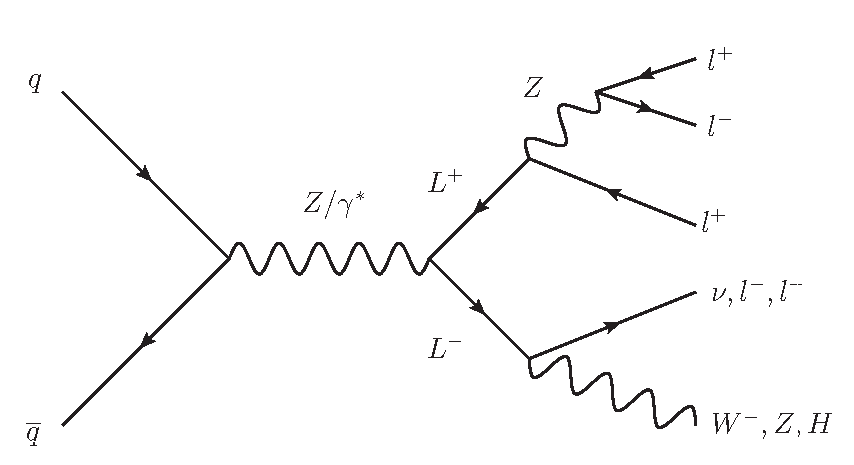
\includegraphics{figures/ch6-resonance/fd_cc2.eps}}
    \label{fig:heavy-lepton-feynman-diagrams-cc}
  }
  \subfloat[ Production of a charged and a neutral heavy lepton.] {
    \resizebox{0.45\textwidth}{!}{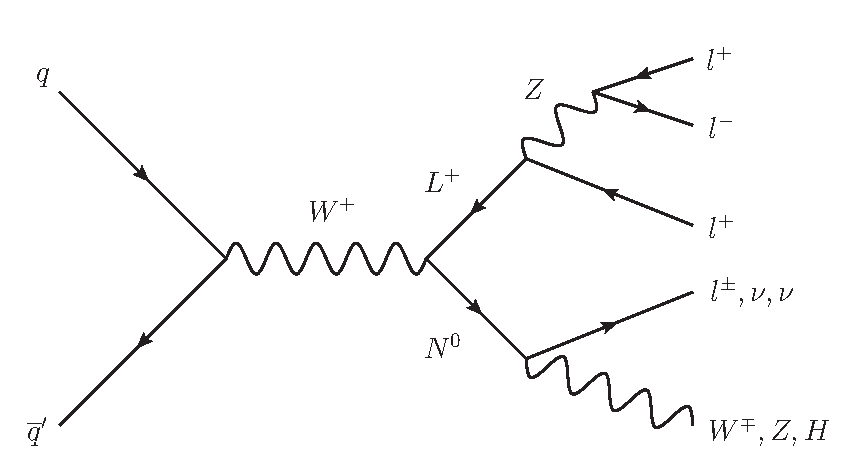
\includegraphics{figures/ch6-resonance/fd_cn2.eps}}
    \label{fig:heavy-lepton-feynman-diagrams-cn}
  }
  \caption{Production and decay of new heavy leptons to final states with a trilepton resonance.}
  \label{fig:heavy-lepton-feynman-diagrams}
\end{figure}

\begin{figure}[htbp]
	\centering
	\subfloat[ Type III Seesaw] {
		\resizebox{0.45\textwidth}{!}{\includegraphics{figures/ch6-resonance/c_xsec_t3ss.png}}
	}
	\hfill
	\subfloat[ Vector-Like Leptons] {
		\resizebox{0.45\textwidth}{!}{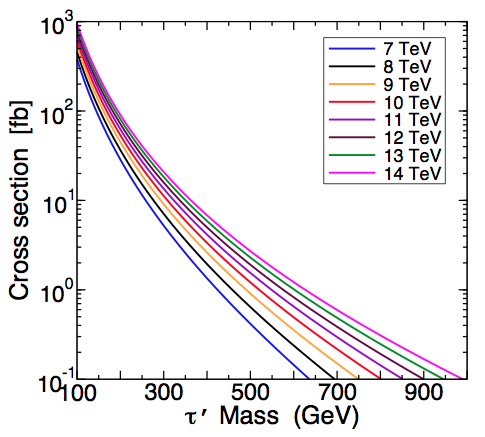
\includegraphics{figures/ch6-resonance/vll_xsec.png}}
	}
	\caption{Production cross sections at $\sqrt{s}=8 \TeV$ for heavy lepton pair production for the type~III seesaw model (left) and the vector-like leptons model (right).}
	\label{fig:resonance-production-cross-sections}
\end{figure}


The heavy leptons are made unstable by introducing mixing terms with the Standard Model leptons. For example, consider a single extra generation of fermions transforming in the adjoint representation of $\mathrm{SU}(2)_L$, as in the type~III seesaw model: $\Sigma\equiv \left(\begin{array}{cc} \lzero/\sqrt{2} & \Sigma^+ \\ \Sigma^- & -\lzero/\sqrt{2}\end{array}\right)$~\cite{Abada:2008ea,Biggio:2011ja}. The Lagrangian contains Yukawa terms mixing the heavy leptons with Standard Model leptons:
\begin{equation}
  -\mathcal{L} \ni \sum_{l=e,\mu,\tau} \sqrt{2}\phi^0 \overline{\Psi} Y_{\lpm l} l_L + \mathrm{h.c.},
\end{equation}
where $\Psi\equiv \Sigma^{+c}_R + \Sigma^-_R$ is a Dirac spinor representating the four charged degrees of freedom, $\phi\equiv(\phi^+,\phi^0)^T\equiv (\phi^+,(v+H+i\eta)/\sqrt{2})^T$ is the Higgs doublet, $Y_{\lpm l}$ are Yukawa couplings, and $l_L$ is a Standard Model lepton. After electroweak symmetry breaking, the mass matrices take the form
\begin{equation}
-\mathcal{L} \ni \sum_{l=e,\mu,\tau} \left(\begin{array}{cc}\overline{l}_R & \overline{\Psi}_R \end{array} \right) \left(\begin{array}{cc} m_l & 0 \\ Y_{\lpm l}v & M_{\lpm} \end{array}\right) \left(\begin{array}{c} l_L \\ \Psi_L \end{array}\right)  + \left(\begin{array}{cc}\overline{l}_L & \overline{\Psi}_L\end{array}\right) \left(\begin{array}{cc} m_l & Y_{\lpm l}^{\dagger}v \\ 0 & M_{\lpm} \end{array}\right) \left(\begin{array}{c} l_R \\ \Psi_r \end{array}\right).
\end{equation}

Diagonalizing the mass matrices leads to off-diagonal terms in the gauge interactions, with couplings proportional to the mixing parameters $V_{\alpha\Sigma}=\frac{v}{\sqrt{2}} M_{\lpm}^{-1} Y_{\alpha\Sigma}$. These couplings enable the decay of the heavy leptons to a boson ($W$, $Z$, or $h$) plus a Standard Model lepton or neutrino, with partial widths given by:

%
\begin{align}
\label{eq:Gammatr0W}
\Gamma(\lzero \to l_\alpha^- W^+) &=  \Gamma(\lzero \to l_\alpha^+ W^-) =
\frac{g^2}{64 \pi} |V_{\alpha\Sigma}|^2
\frac{M_{\lpm}^3}{M_W^2} \left( 1- \frac{M_W^2}{M_{\lpm}^2} \right)^2 
\left( 1 + 2 \frac{M_W^2}{M_{\lpm}^2} \right) , 
\\[0.1cm]
\label{eq:Gammatr0Z}
\sum_l\Gamma(\lzero \to \nu_l Z) &=  \frac{g^2}{64 \pi c_W^2} 
\sum_\alpha |V_{\alpha\Sigma}|^2
\frac{M_{\lpm}^3}{M_Z^2} \left( 1- \frac{M_Z^2}{M_{\lpm}^2} \right)^2 
\left( 1 + 2 \frac{M_Z^2}{M_{\lpm}^2}\right),
\\[0.2cm]
\label{eq:Gammatr0h}
\sum_l\Gamma(\lzero \to \nu_l H) &=  \frac{g^2}{64 \pi} 
\sum_\alpha |V_{\alpha\Sigma}|^2
\frac{M_{\lpm}^3}{M_W^2} \left( 1- \frac{M_H^2}{M_{\lpm}^2} \right)^2 ,
\\[0.2cm]
\label{eq:Gammatr+W}
\sum_l\Gamma(\Sigma^+ \to \nu_l W^+) &= 
\frac{g^2}{32 \pi} \sum_\alpha |V_{\alpha\Sigma}|^2
\frac{M_{\lpm}^3}{M_W^2} \left( 1- \frac{M_W^2}{M_{\lpm}^2} \right)^2 
\left( 1 + 2 \frac{M_W^2}{M_{\lpm}^2} \right) ,
\\[0.2cm]
\label{eq:Gammatr+Z}
\Gamma(\Sigma^+ \to l_\alpha^+ Z) &= 
\frac{g^2}{64 \pi c_W^2} |V_{\alpha\Sigma}|^2
\frac{M_{\lpm}^3}{M_Z^2} \left( 1- \frac{M_Z^2}{M_{\lpm}^2} \right)^2 
\left( 1 + 2 \frac{M_Z^2}{M_{\lpm}^2}\right),
\\[0.2cm]
\label{eq:Gammatr+h}
\Gamma(\Sigma^+ \to l_\alpha^+ H) &= \frac{g^2}{64 \pi} |V_{\alpha\Sigma}|^2
\frac{M_{\lpm}^3}{M_W^2} \left( 1- \frac{M_H^2}{M_{\lpm}^2} \right)^2 .
\end{align}

where $\alpha$ and $l$ run over Standard Model lepton and neutrino generations. The branching fractions of the charged and neutrino heavy leptons are shown as function of $m_{\lpm}$ in figure~\ref{fig:resonance-branching-ratios}. Note that these branching fractions are common to all the models considered in this analysis (aside from the possibility of only having a charged heavy lepton).


\begin{figure}[h]
  \centering
  \subfloat[ Charged heavy fermion] {
    \resizebox{0.45\textwidth}{!}{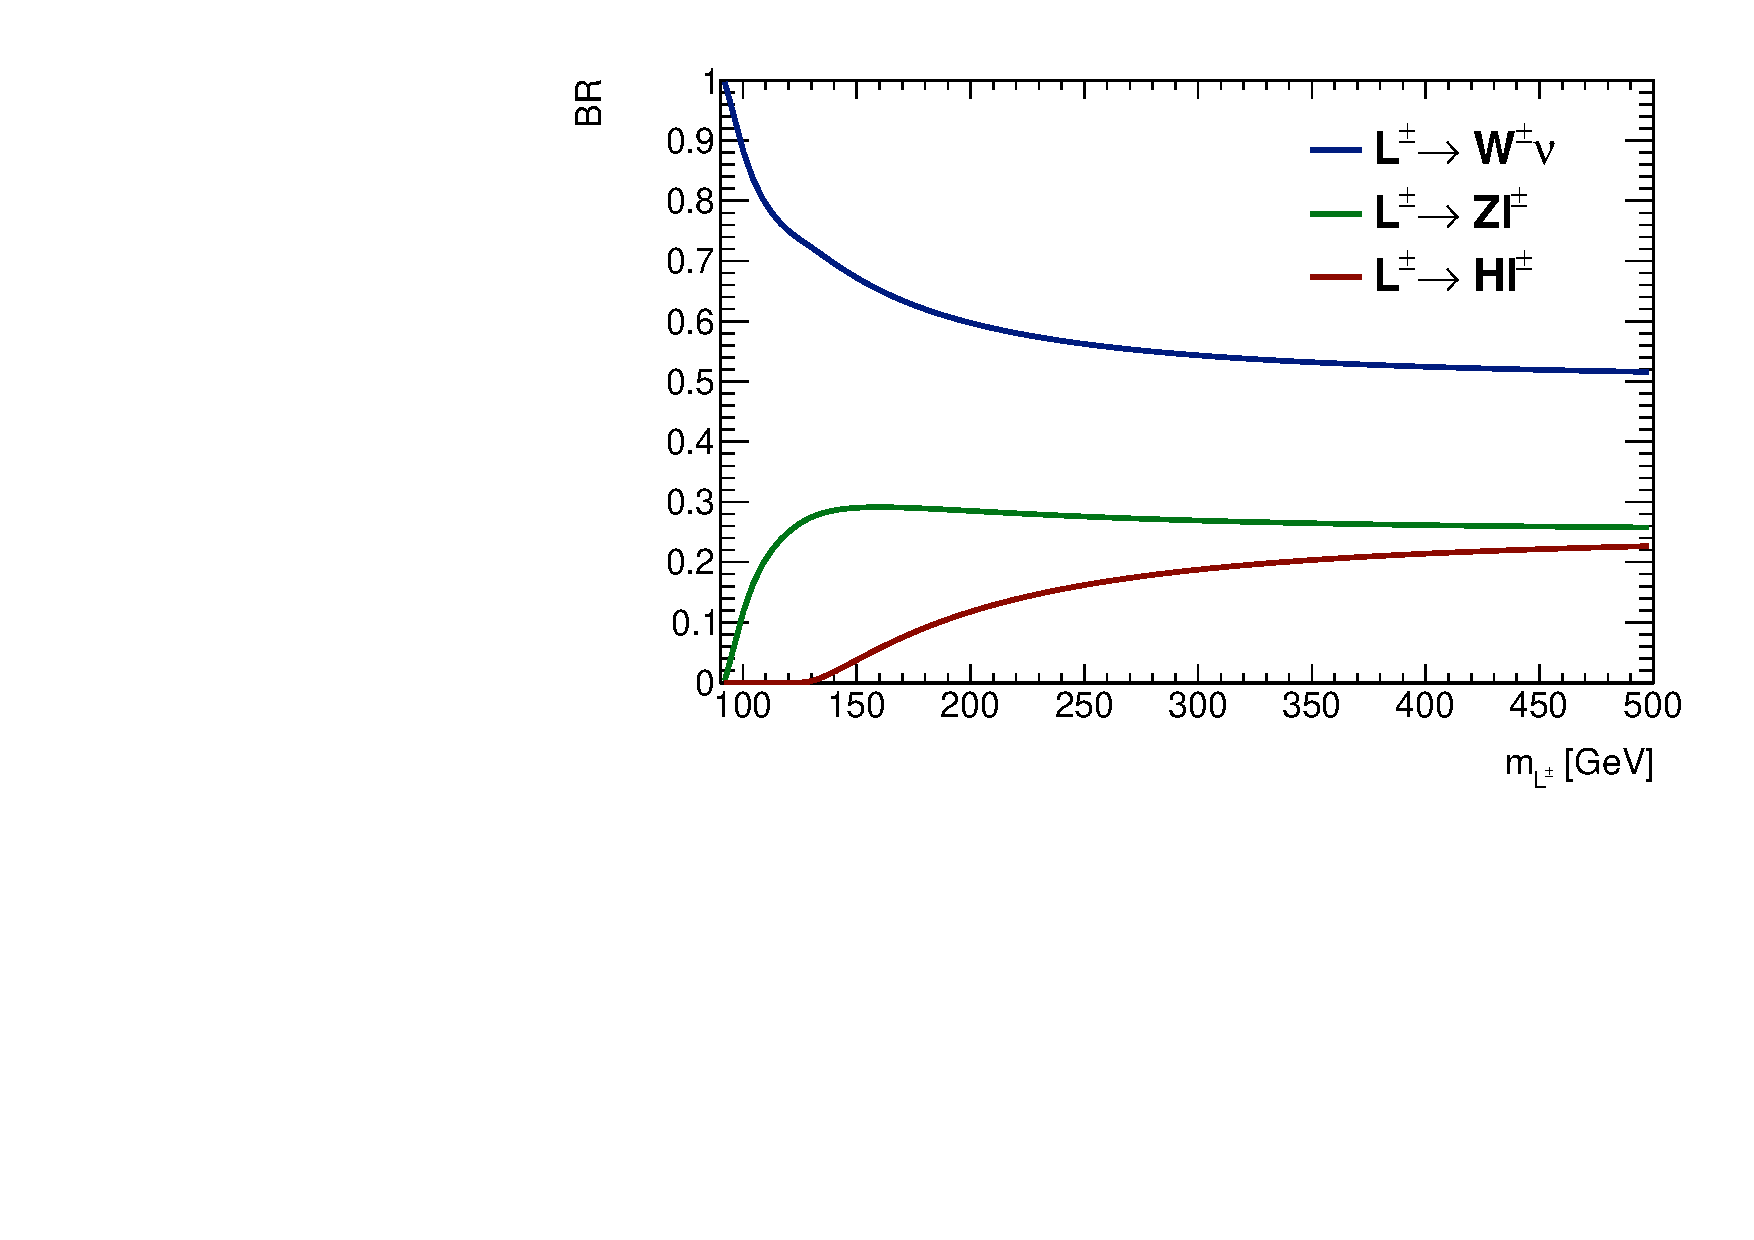
\includegraphics{figures/ch6-resonance/c_br_charged}}
  }
  \subfloat[ Neutral heavy fermion] {
    \resizebox{0.45\textwidth}{!}{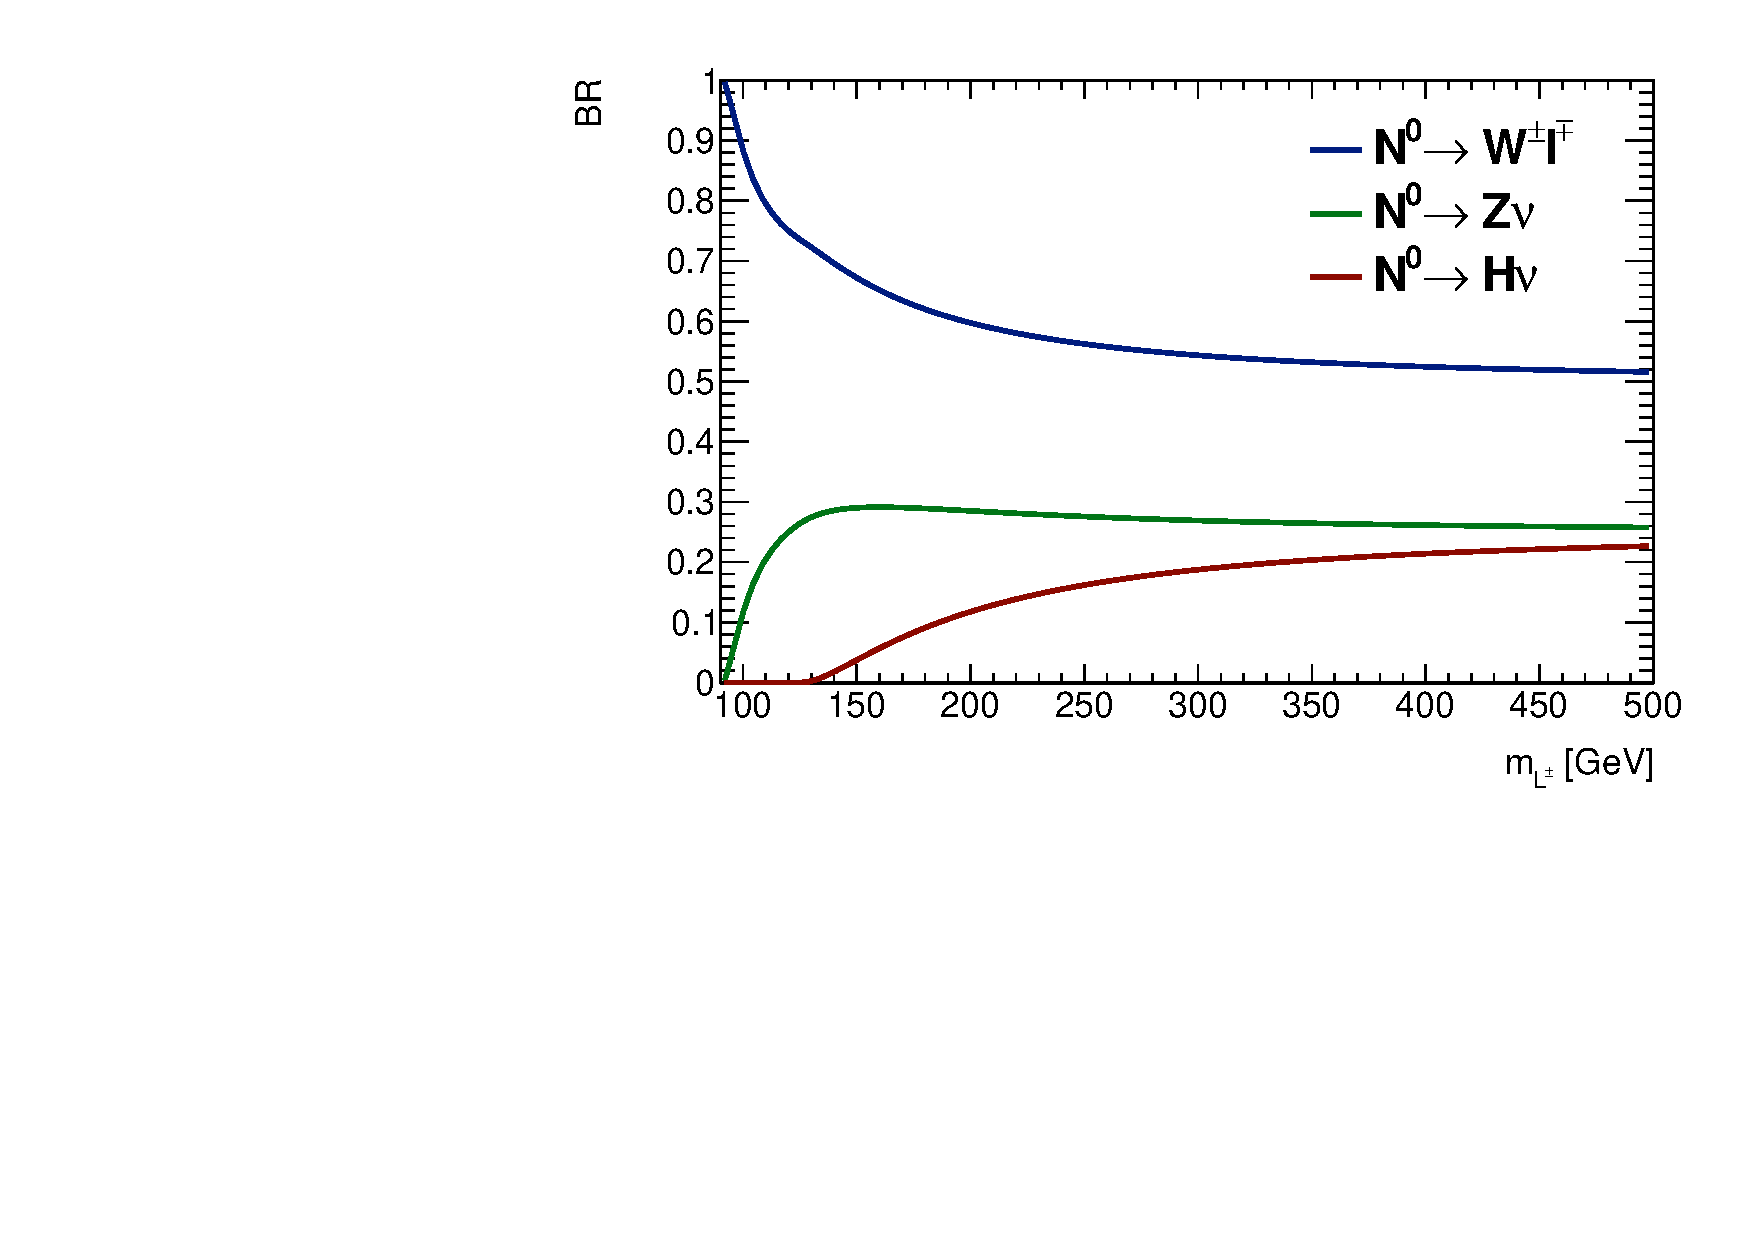
\includegraphics{figures/ch6-resonance/c_br_neutral}}
  }
  \caption{Branching ratios of a heavy lepton decaying via mixing with Standard Model leptons~\cite{Biggio:2011ja}.}
  \label{fig:resonance-branching-ratios}
\end{figure}

Constraints on the mixing parameters $V_i$ can be derived from precision measurements of the $Z$ width, and constraints on products of the mixing parameters from flavor violation experiments like $\mu\rightarrow e\gamma$~\cite{Abada:2008ea,Abada:2007ux,delAguila:2008pw,Altmannshofer:2013zba}:

\begin{align}
|V_{e L}| & <5.5\times10^{-2}\\
|V_{\mu L}| & <6.3\times10^{-2}\\
|V_{\tau L}| & <6.3\times10^{-2}\\
|V_{e L}V_{\mu L}| & <1.7\times10^{-7}\\
|V_{e L}V_{\tau L}| & <4.2\times10^{-4}\\
|V_{\mu L}V_{\tau L}| & <4.9\times10^{-4}
\end{align}

\subsection{Signal Monte Carlo Samples}\label{sec:resonance-signal-mc-samples}

Signal events are generated using Monte Carlo simulation, at eleven mass hypotheses in the range $100 \GeV \leq m_{\lpm} \leq 400 \GeV$ for the vector-like leptons model and ten mass hypothesis in the range $100 \GeV \leq m_{\lpm,\lzero}\leq 500 \GeV$ for the type~III seesaw model. The samples are summarized in table~\ref{table:resonance-signal-samples}. The events are generated with \madgraph~4.5.2 and 5.2.2.1~\cite{madgraph}, for the vector-like leptons and type~III seesaw models, respectively, using the CTEQ6L1\cite{ct6l1} parton distribution functions (PDF) and the AU2 underlying event tune~\cite{AU2}. Showering is performed with \pythia\ 8~\cite{Sjostrand:2007gs}. Decays of the heavy leptons in the vector-like leptons model are performed using \bridge~\cite{bridge}, while decays in the type~III seesaw samples are performed by \madgraph. The cross sections for both samples are calculated at leading order (LO) in QCD, and are shown in table~\ref{table:resonance-signal-samples}. 

For the type~III seesaw model, the charged and neutral heavy leptons are generated with identical masses. The simulated decay modes are listed in table~\ref{table:resonance-seesaw-sample-decays}. The mixing parameters are chosen to be $V_e=0.055$, $V_{\mu}=0.063$, and $V_{\tau}=0$, yielding a mix of $ee$, $e\mu$, and $\mu\mu$ decays. For the vector-like leptons model, one heavy lepton is required to decay via $L^{\pm}\rightarrow Z(\ell\ell)\ell$, where $\ell=e,\mu,\tau$. The two heavy leptons are constrained to decay to the same flavor of Standard Model lepton, which is chosen with equal probability to be an electron, muon, or tau. For both models, the events are divided and reweighted to correspond to electron-only or muon-only mixing scenarios. 

The type~III seesaw samples were simulated with no intrinsic width for the $Z$ bosons. As a result, the signal peaks are slightly narrower than would be expected if the $Z$ width were correctly included. As described below in section~\ref{sec:resonance-signal-model}, the limit setting is performed by fitting the $\deltam$ distributions with analytical functions. In order to incorporate the $Z$ width into the signal peaks, the peak width parameters of the vector-like lepton peaks are used for the type~III seesaw model. 


\begin{table}[htbp]
	\centering
	\resizebox{\textwidth}{!}{
		\begin{tabular}{|l||c|c|c|c|r|}
			\hline
			Mass [GeV] & Dataset ID  & Cross Section [pb] & Filter Efficiency & Number of Events \\
			\hline
			\multicolumn{5}{c}{Type III Seesaw} \\
			\hline
			100	&	191030	 	&	1.273		&	0.1018	&	100,000 \\
			\hline
			120	&	191031	 	&	2.138		&	0.1628	&	100,000 \\
			\hline
			160	&	191032	 	&	0.853		&	0.1808	&	100,000 \\
			\hline
			200	&	191033	 	&	0.346		&	0.2012	&	100,000 \\
			\hline
			250	&	191034	 	&	0.135		&	0.2096	&	100,000 \\
			\hline
			300	&	191035	 	&	0.0604		&	0.2178	&	50,000 	\\
			\hline
			350	&	191036	 	&	0.02969		&	0.2337	&	50,000 	\\
			\hline
			400	&	191037	 	&	0.01566		&	0.2409	&	50,000 	\\
			\hline
			450	&	191038	 	&	0.008733	&	0.2456	&	50,000 	\\
			\hline
			500	&	191039	 	&	0.00504		&	0.2493	&	50,000 	\\
			\hline
			\hline
			\multicolumn{5}{c}{Vector-Like Leptons} \\
			\hline
			100	&	180579	&	0.378 	&	0.0233	& 100,000 \\
			\hline
			110	&	180580	&	0.264 	&	0.0412	& 100,000 \\
			\hline
			120	&	180581	&	0.193 	&	0.0498	& 100,000 \\
			\hline
			130	&	180582	&	0.142 	&	0.0548	& 100,000 \\
			\hline
			140	&	180583	&	0.106 	&	0.0569	& 100,000 \\
			\hline
			160	&	180584	&	0.0645 	&	0.0579	& 100,000 \\
			\hline
			180	&	180585	&	0.0407 	&	0.0575	& 100,000 \\
			\hline
			200	&	180586	&	0.0265 	&	0.0567	& 100,000 \\
			\hline
			250	&	180587	&	0.0104 	&	0.0548	& 100,000 \\
			\hline
			300	&	180588	&	0.00457	&	0.0536	& 100,000 \\
			\hline
			400	&	180589	&	0.00115	&	0.0520	& 100,000 \\
			\hline
		\end{tabular}
	}
	\caption{Summary of signal Monte Carlo samples. Ten mass points are simulated for the type~III seesaw model, and eleven for the vector-like leptons model.}
	\label{table:resonance-signal-samples}
\end{table}

\begin{table}
	\centering
	\begin{tabular}{c|ll}
		Production Mode & Decay 1 & Decay 2 \\
		\hline
		$pp \rightarrow \lzero\Sigma^{+}$	&	$\lzero \rightarrow l^{+} W^{-}$	&	$\Sigma^{+} \rightarrow l^{+} Z$ \\
		$pp \rightarrow \lzero\Sigma^{+}$	&	$\lzero \rightarrow l^{-} W^{+}$	&	$\Sigma^{+} \rightarrow l^{+} Z$ \\
		$pp \rightarrow \lzero\Sigma^{+}$	&	$\lzero \rightarrow \nu_{l} Z$		&	$\Sigma^{+} \rightarrow l^{+} Z$ \\
		$pp \rightarrow \lzero\Sigma^{+}$	&	$\lzero \rightarrow \nu_{l} H$		&	$\Sigma^{+} \rightarrow l^{+} Z$ \\
		$pp \rightarrow \lzero\Sigma^{-}$	&	$\lzero \rightarrow l^{-} W^{+}$	&	$\Sigma^{-} \rightarrow l^{-} Z$ \\
		$pp \rightarrow \lzero\Sigma^{-}$	&	$\lzero \rightarrow l^{+} W^{-}$	&	$\Sigma^{-} \rightarrow l^{-} Z$ \\
		$pp \rightarrow \lzero\Sigma^{-}$	&	$\lzero \rightarrow \nu_{l} Z$		&	$\Sigma^{-} \rightarrow l^{-} Z$ \\
		$pp \rightarrow \lzero\Sigma^{-}$	&	$\lzero \rightarrow \nu_{l} H$		&	$\Sigma^{-} \rightarrow l^{-} Z$ \\
		$pp \rightarrow \Sigma^{-}\Sigma^{+}$	&	$\Sigma^{-} \rightarrow l^{-} Z$		&	$\Sigma^{+} \rightarrow l^{+} Z$ \\
		$pp \rightarrow \Sigma^{-}\Sigma^{+}$	&	$\Sigma^{-} \rightarrow \nu_{l} W^{-}$	&	$\Sigma^{+} \rightarrow l^{+} Z$ \\
		$pp \rightarrow \Sigma^{-}\Sigma^{+}$	&	$\Sigma^{-} \rightarrow l^{-} H$		&	$\Sigma^{+} \rightarrow l^{+} Z$ \\
		$pp \rightarrow \Sigma^{-}\Sigma^{+}$	&	$\Sigma^{-} \rightarrow l^{-} Z$		&	$\Sigma^{+} \rightarrow \nu_{l} W^{+}$ \\
		$pp \rightarrow \Sigma^{-}\Sigma^{+}$	&	$\Sigma^{-} \rightarrow l^{-} Z$		&	$\Sigma^{+} \rightarrow l^{+} H$ \\
	\end{tabular}
	\caption{Decays simulated for the type~III seesaw signal samples.}
	\label{table:resonance-seesaw-sample-decays}
\end{table}



\section{Search Strategy}\label{sec:resonance-search-strategy}
\subsection{Event Selection and Heavy Lepton Reconstruction}\label{sec:event-3l-selection}
The event selection is very similar to that used in the model-independent analysis, described in section~\ref{sec:model-independent-event-selection}. In particular, the same definitions are used for leptons and jets, in order to make use of the same fake factor method to estimate the reducible backgrounds. Events containing a heavy lepton candidate are selected as follows.

\begin{itemize}
	\item Events are triggered using the lowest-threshold unprescaled single-electron and single-muon triggers, \texttt{EF\_e24vhi\_medium1}, \texttt{EF\_e60\_medium1}, \texttt{EF\_mu24i\_tight}, and \texttt{EF\_mu36\_tight}.
	\item The primary event vertex must have at least three tracks with $\pt>400~\mbox{MeV}$.
	\item Events are required to have at least three electrons or muons ($eee$, $ee\mu$, $\mu\mu e$, $\mu\mu\mu$) satisfying the lepton cuts (table~\ref{table:lepton-selections}). 
	\item Events must have one $Z$ candidate, consisting of a same-flavor, opposite-sign pair of leptons with $|m_{l^+l^-}-m_{Z}|<10~\mbox{GeV}$. The $Z$ mass is taken to be $m_Z=91.1876~\mbox{GeV}$~\cite{PhysRevD.86.010001}. 
	\item Four-lepton events with two leptonic $Z$ candidates are rejected to suppresses background from $ZZ$ events. The efficiency loss for signal events is low, in part due to the additional factor of the leptonic branching ratio of the $Z$; see tables~\ref{table:fiducial-efficiencies-Ze} and \ref{table:fiducial-efficiencies-Zmu}. 
	\item If an event contains more than three leptons, a unique trilepton candidate in each event is chosen as follows:
	\begin{itemize}
		\item Choose the same-flavor, opposite-sign (SFOS) pair with invariant mass closest to $m_{Z}$.
		\item Choose the third (``off-$Z$'') lepton to be the closest in $\Delta R$ to the reconstructed $Z$ four-momentum.
	\end{itemize}
	\item For low heavy lepton mass hypotheses, $m_{\lpm}\lesssim 200~\mbox{GeV}$, the $Z$ and the third lepton will tend to be collimated. The expected background and signal $\Delta R$ distributions for selected trilepton candidate are shown in figure~\ref{fig:resonance-inclusive-dR}. Imposing a cut on the $\Delta R(Z,\ l_3)$ of the trilepton candidates improves the signal significance, and also provides a useful control region defined by inverting the cut.

	\begin{figure}[h]
		\centering
		\resizebox{0.6\textwidth}{!}{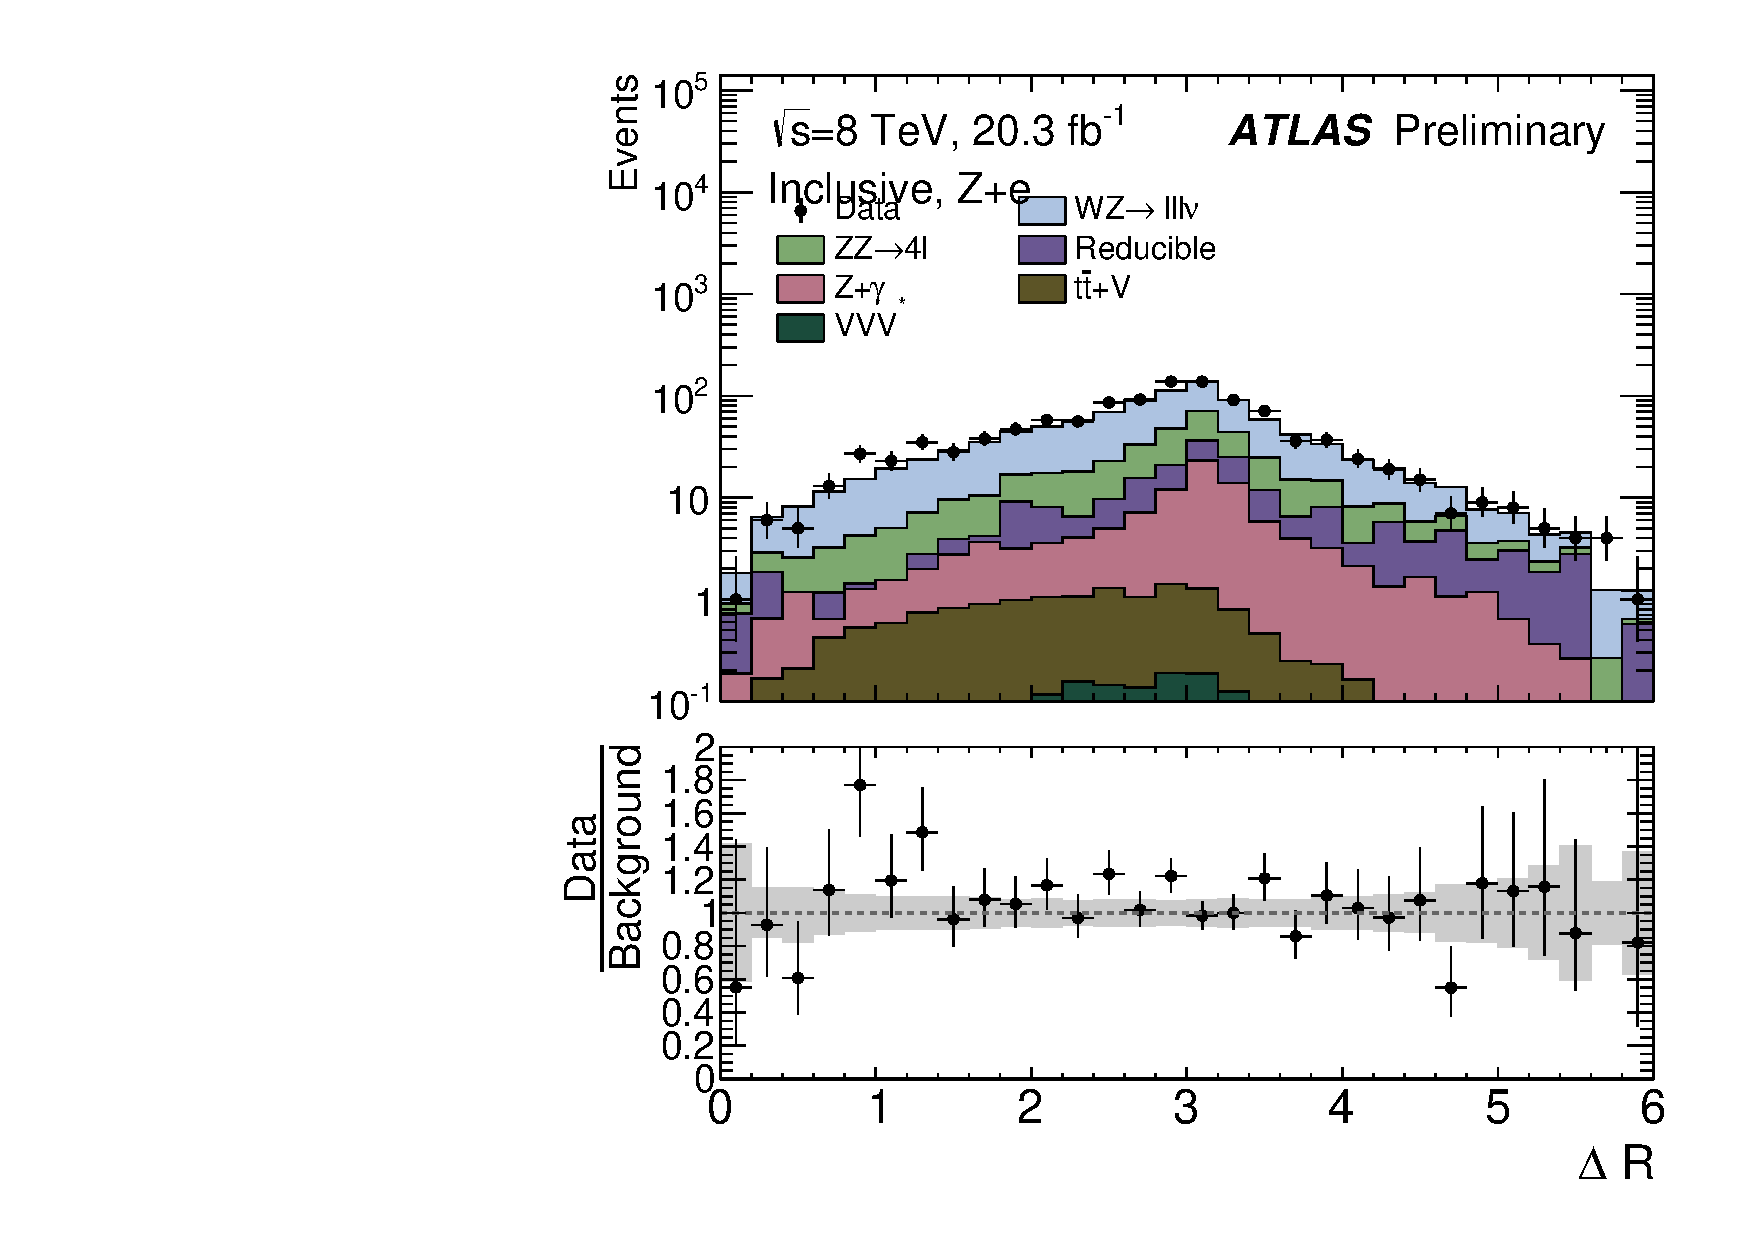
\includegraphics{figures/ch6-resonance/c_output_dR_Ze_InclusiveNoM3LDeltaR_300GeV_log}}
		\caption{Expected $\Delta R(Z,\ l_3)$ distributions for background and signal in the inclusive signal region.}
		\label{fig:resonance-inclusive-dR}
	\end{figure}
  
	The cut on $\Delta R(Z,\ l_3)$ is chosen by running the cut-and-count based limit setting, described in section~\ref{sec:limit-method-mass-windows}, with different values of the $\Delta R$ cut. For cut values of $\Delta R < 2.0,\ 2.25,\ 2.5,\ 2.75,\ 3.0,\ 3.14,\ 3.5,$ and $4.0$, the expected exclusions were determined using \texttt{mclimits}, based on the expected signal and background yields in narrow mass windows around the signal mass hypotheses. For simplicity, the same $\Delta R(Z,\ l_3)$ cut is applied to all categories; no significant gain is observed by optimizing each category individually. The expected exclusions for different $\Delta R(Z,\ l_3)$ cuts are shown in figure~\ref{fig:dR-optimization}. Smaller values of the cut ($\Delta R(Z,\ l_3)\lesssim 2.0$) perform similarly to more stringent cuts at low signal mass hypotheses, but decline at higher mass hypotheses. Cuts above $\Delta R(Z,\ l_3)\lesssim 3.0$ perform approximately equally. Based on these studies, and also to use the inverse of this cut to define a control region, a cut value of $\Delta R(Z,\ l_3)<3.0$ is chosen. 

	\begin{figure}[h]
		\subfloat[Vector-Like Leptons] {
			\resizebox{0.45\textwidth}{!}{\includegraphics{figures/ch6-resonance/{c_limits_dRVariation_VLL_Combined_BRe1.0_BRmu0.0}.pdf}}
		}
		\subfloat[Seesaw] {
			\resizebox{0.45\textwidth}{!}{\includegraphics{figures/ch6-resonance/{c_limits_dRVariation_Seesaw_Combined_BRe1.0_BRmu0.0}.pdf}}
		}
		\caption{Expected upper limits on cross section times branching ratio to final states with least one trilepton resonant decay for different cuts on $\Delta R(Z,\ l_3)$.}
		\label{fig:dR-optimization}
	\end{figure}

	\item The variable of interested used to apply the trilepton mass constraint is $\Delta m \equiv m_{3\ell}-m_{\ell^+\ell^-}$, where the invariant mass of the two leptons associated with a $Z$ boson decay is subtracted by the trilepton mass. This method reduces the impact of the lepton energy or momentum resolutions on the width of the resonance peak, at the cost of introducing some width due to the intrinsic width of the $Z$, $\Gamma_Z=2.4952\pm0.0023 \GeV$~\cite{pdg}. Over most of the mass range, this variable reduces the width of the signal peaks, as shown in figure~\ref{fig:deltam-m3l-comparison}. 

	\begin{figure}[htbp]
		\textcolor{red}{m3l deltam comparison plot or table}
		\caption{Comparison of the full-width, half-maximum of the signal peaks between the $\deltam$ and $m_{3l}$ variables.}
		\label{fig:deltam-m3l-comparison}
	\end{figure}
	  
\end{itemize}

After identifying the trilepton candidates, six mutually exclusive signal regions are defined. First, to target the flavor structure of the heavy lepton mixing, events are divided into two flavor channels, $Z+e$ and $Z+\mu$, depending on the flavor the off-$Z$ lepton. Second, as the heavy leptons are pair produced, signal events will contain additional activity due to the decay of the second heavy lepton. Events are divided into three exclusive categories based on other activity in the event:
  \begin{itemize}
  	\item \textbf{\fourl}: Event contains a fourth lepton, either an electron or a muon, passing the normal lepton criteria. 
  	\item \textbf{\threeljj}: Event contains exactly three leptons, and a dijet with $60.385~\mbox{GeV}<m_{jj}<150.9~\mbox{GeV}$. 
  	\item \textbf{\threelo}: All other events, i.e. events with three leptons and no jet pair satisying the invariant mass requirement. 
  \end{itemize}

 The division into the three signal regions targeting the opposite side decay is motivated in figure~\ref{fig:opposite-side-br}, which shows the fraction of events with various activity from the decay of the other heavy lepton. The additional activity includes extra leptons and neutrinos, and jets from $W/Z/h$ decays. The requirement of either a fourth lepton or a hadronically decaying boson is very efficient on signal: if the second heavy fermion is charged, then every decay satisfies this requirement, while if the second heavy fermion is neutral, then every decay except for $\Sigma^0\rightarrow Z\nu\rightarrow \nu\nu\nu$ and decays to Higgs bosons satisfies this requirement. Categorization targeting neutrinos is less effective at separating signal from the large $WZ$ background (see figures~\ref{fig:SR-mTW-1}-\ref{fig:SR-ETMiss-2}). 

In some cases, it is useful to consider the events without dividing into these three categories, but rather only the flavor of the off-$Z$ lepton. This is referred to as the ``Inclusive'' signal region below.

\begin{figure}
	\subfloat[ $\lpm$] {
		\resizebox{0.48\textwidth}{!}{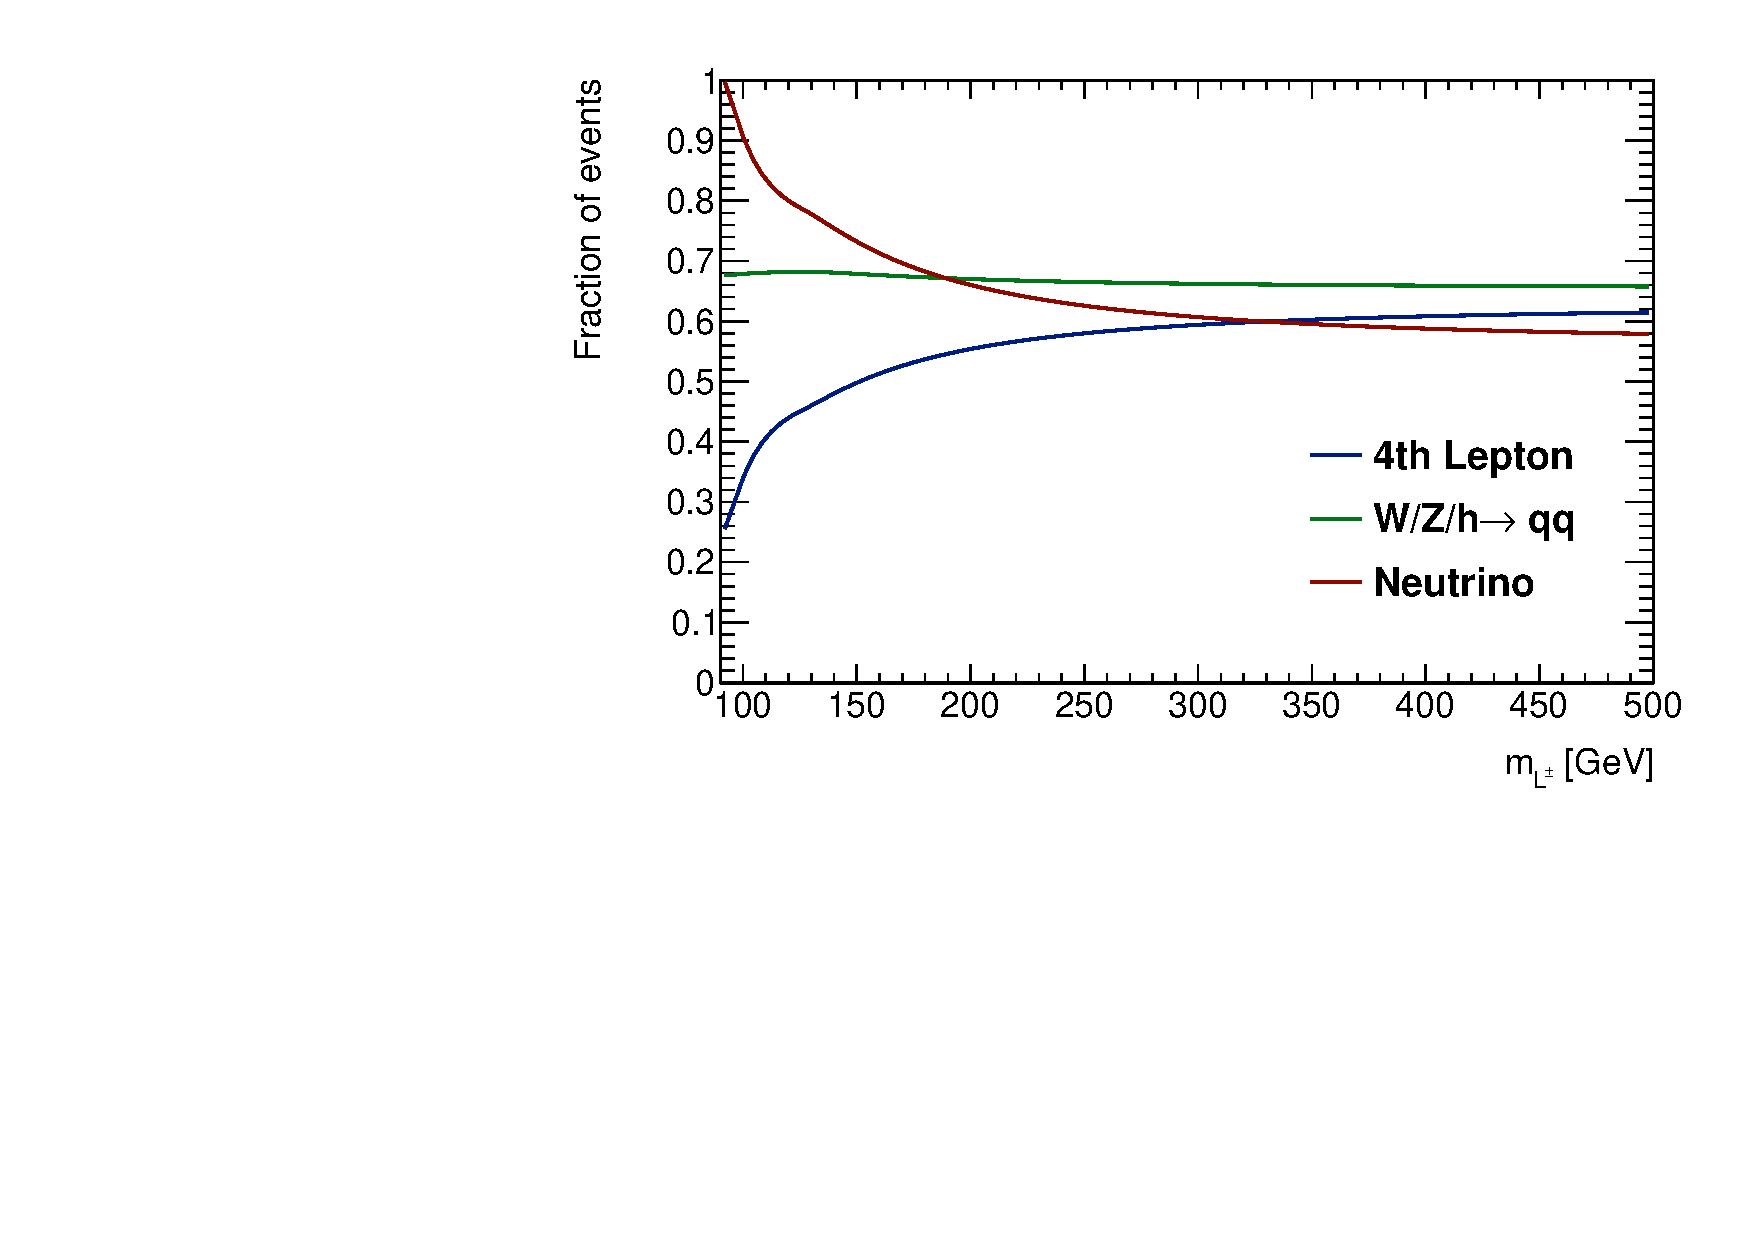
\includegraphics{figures/ch6-resonance/c_oppositesideactivity_charged.pdf}}
	}
	\subfloat[ $\lzero$] {
		\resizebox{0.48\textwidth}{!}{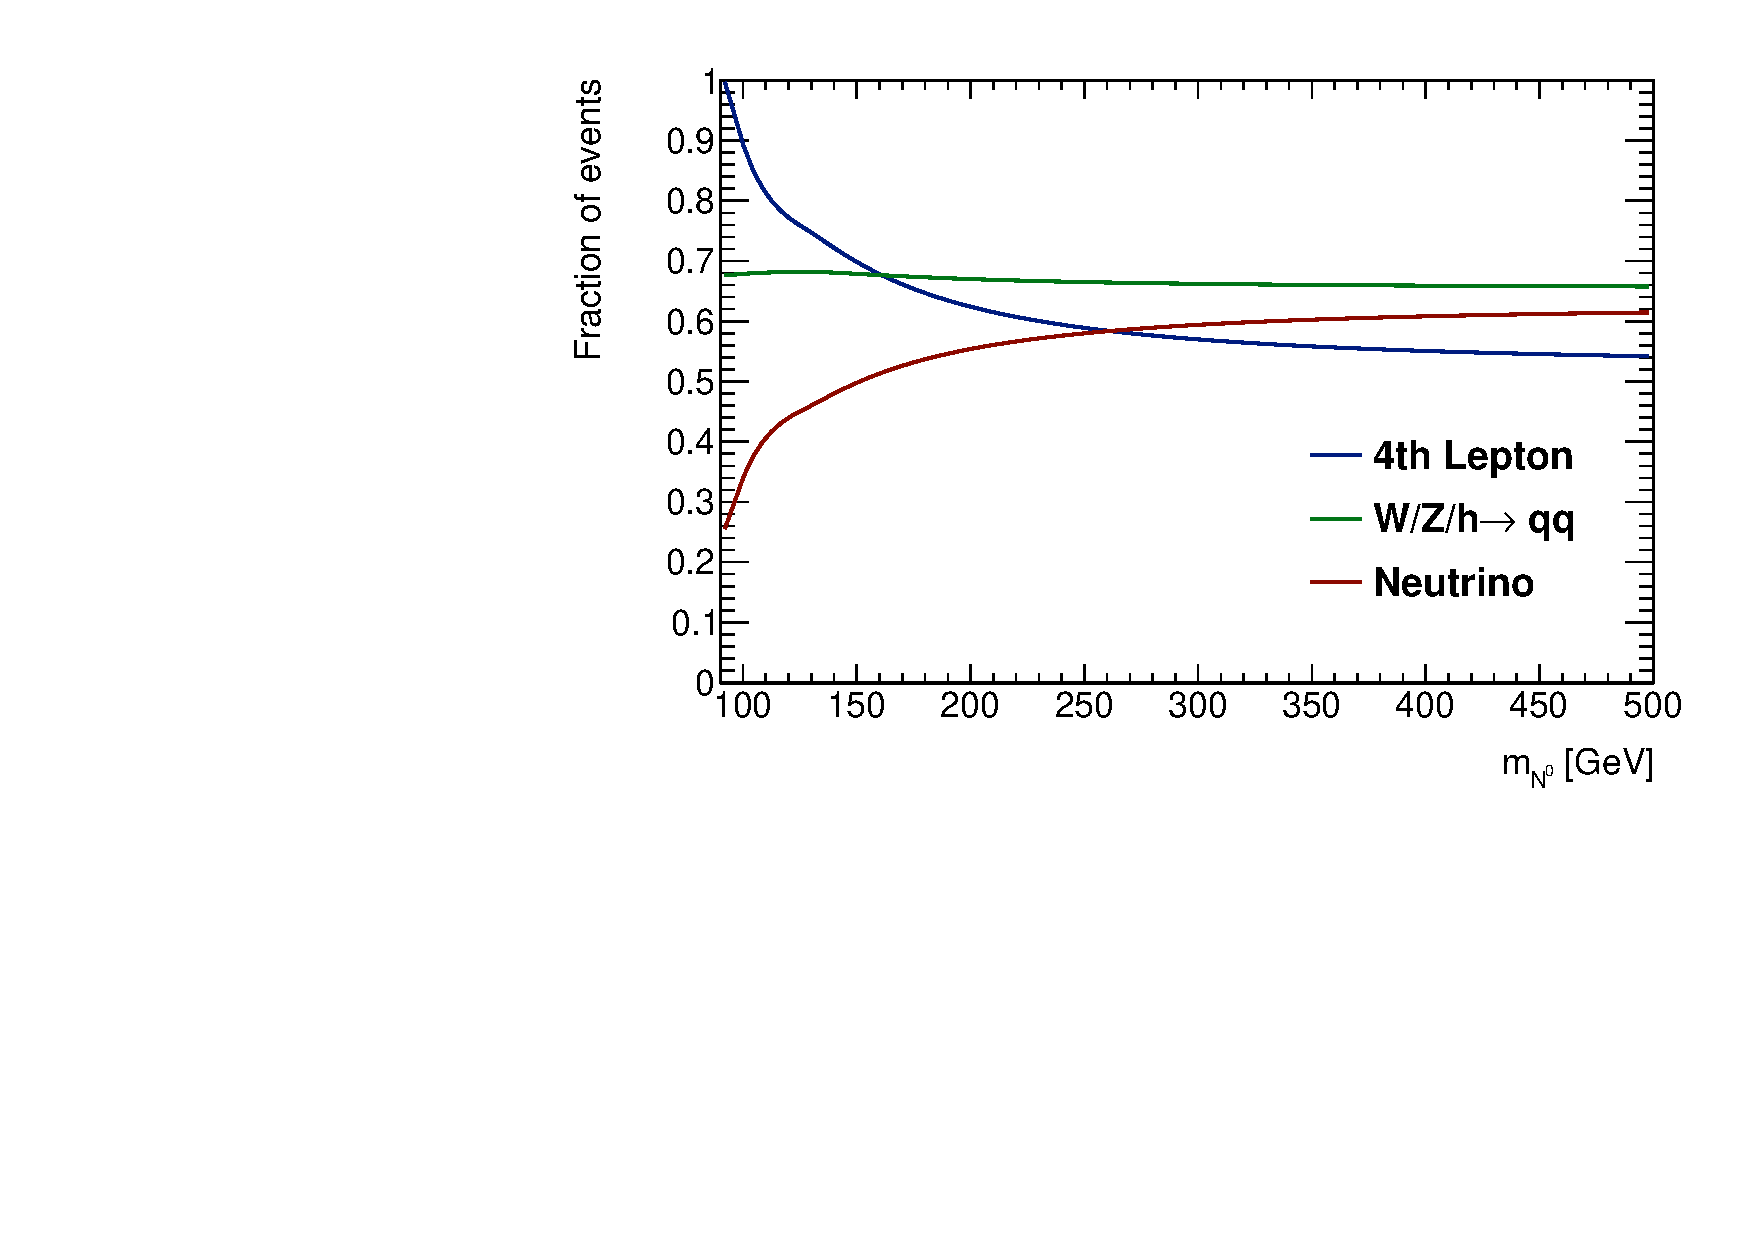
\includegraphics{figures/ch6-resonance/c_oppositesideactivity_neutral.pdf}}
	}
	\caption{Fraction of events with various activity on the opposite side of the event, for $\lpm\Sigma^{\mp}$ events at left, and $\lpm\Sigma^0$ events at right. The left plot, showing the opposite side activity for a $\lpm\Sigma^{\mp}$ final state, is identical for the seesaw and vector-like lepton model.
	}
	\label{fig:opposite-side-br}
\end{figure}

\subsection{Performance on Fiducial Signal Events}\label{sec:fiducial-cutflow}
The performance of the cuts and heavy lepton candidate selection is shown in tables~\ref{table:fiducial-efficiencies-Ze} and \ref{table:fiducial-efficiencies-Zmu} in terms of efficiency on fiducial events. The final efficiency for each signal region is shown as a function of signal mass $m_{\Sigma}$ in figure~\ref{fig:fiducial-efficiencies-vs-mass}. The study is performed separately for the $Z+e$ and $Z+\mu$ flavor channels. The fiducial selection requires the event to have three truth-level leptons satisfying $\pt>15~\mbox{GeV}$ and $|\eta|<2.5$, of which two form a $Z$ candidate with $|m_{l^+l^-}-m_Z|<10~\mbox{GeV}$, the third lepton is of the correct flavor, and the trilepton mass satisfies $|m_{3l}-m_{\lpm}|<5~\mbox{GeV}$.

Note that cut imposing a flavor requirement on the reconstructed off-$Z$ lepton has a different efficiency between the vector-like lepton sample and the seeaw sample. This is a consequence of the initial flavor content of the samples: the vector-like lepton samples are divided into two samples with with 100\% branching fraction to either bachelor electron or bachelor muon, while the seesaw samples is a single mixed sample containing both electron and muon decays. 


\begin{table}[ht]
	\resizebox{\textwidth}{!}{
	\begin{tabular}{|c|c|c|c|c|c||c|c|c|}
		\hline
		Process  & Preselection  & Bachelor $e$  & $|m_{l^{+}l^{-}} - m_{Z}|<10~\mbox{GeV}$  & !$2Z$  & $\Delta R < 3.0$  & $4l$ & $3l+jj$ & Else \\
		\hline
		VLL, $100$~GeV		&	$0.348 \pm 0.008$	&	$0.318 \pm 0.008$	&	$0.306 \pm 0.008$	&	$0.303 \pm 0.008$	&	$0.298 \pm 0.008$	&	$0.054 \pm 0.004$ &	$0.096 \pm 0.005$	&	$0.147 \pm 0.006$	\\
		\hline
		VLL, $110$~GeV		&	$0.478 \pm 0.006$	&	$0.435 \pm 0.006$	&	$0.421 \pm 0.006$	&	$0.417 \pm 0.006$	&	$0.401 \pm 0.006$	&	$0.076 \pm 0.003$ &	$0.11 \pm 0.004$	&	$0.215 \pm 0.005$	\\
		\hline
		VLL, $120$~GeV		&	$0.535 \pm 0.006$	&	$0.491 \pm 0.006$	&	$0.467 \pm 0.006$	&	$0.457 \pm 0.006$	&	$0.424 \pm 0.006$	&	$0.104 \pm 0.004$ &	$0.117 \pm 0.004$	&	$0.204 \pm 0.005$	\\
		\hline
		VLL, $130$~GeV		&	$0.604 \pm 0.006$	&	$0.539 \pm 0.006$	&	$0.509 \pm 0.006$	&	$0.494 \pm 0.006$	&	$0.445 \pm 0.006$	&	$0.125 \pm 0.004$ &	$0.127 \pm 0.004$	&	$0.194 \pm 0.005$	\\
		\hline
		VLL, $140$~GeV		&	$0.643 \pm 0.006$	&	$0.578 \pm 0.006$	&	$0.559 \pm 0.006$	&	$0.538 \pm 0.006$	&	$0.491 \pm 0.006$	&	$0.153 \pm 0.004$ &	$0.164 \pm 0.004$	&	$0.174 \pm 0.005$	\\
		\hline
		VLL, $160$~GeV		&	$0.663 \pm 0.006$	&	$0.593 \pm 0.006$	&	$0.572 \pm 0.006$	&	$0.552 \pm 0.006$	&	$0.499 \pm 0.006$	&	$0.175 \pm 0.005$ &	$0.148 \pm 0.004$	&	$0.176 \pm 0.005$	\\
		\hline
		VLL, $180$~GeV		&	$0.698 \pm 0.006$	&	$0.62 \pm 0.006$	&	$0.594 \pm 0.006$	&	$0.573 \pm 0.007$	&	$0.505 \pm 0.007$	&	$0.197 \pm 0.005$ &	$0.163 \pm 0.005$	&	$0.144 \pm 0.005$	\\
		\hline
		VLL, $200$~GeV		&	$0.707 \pm 0.006$	&	$0.624 \pm 0.007$	&	$0.596 \pm 0.007$	&	$0.577 \pm 0.007$	&	$0.52 \pm 0.007$	&	$0.209 \pm 0.006$ &	$0.167 \pm 0.005$	&	$0.145 \pm 0.005$	\\
		\hline
		VLL, $250$~GeV		&	$0.751 \pm 0.007$	&	$0.654 \pm 0.007$	&	$0.626 \pm 0.007$	&	$0.615 \pm 0.007$	&	$0.548 \pm 0.008$	&	$0.245 \pm 0.007$ &	$0.152 \pm 0.005$	&	$0.151 \pm 0.005$	\\
		\hline
		VLL, $300$~GeV		&	$0.771 \pm 0.007$	&	$0.662 \pm 0.008$	&	$0.63 \pm 0.008$	&	$0.625 \pm 0.008$	&	$0.547 \pm 0.008$	&	$0.258 \pm 0.007$ &	$0.169 \pm 0.006$	&	$0.121 \pm 0.005$	\\
		\hline
		VLL, $400$~GeV		&	$0.776 \pm 0.007$	&	$0.669 \pm 0.008$	&	$0.642 \pm 0.008$	&	$0.641 \pm 0.008$	&	$0.562 \pm 0.008$	&	$0.277 \pm 0.007$ &	$0.181 \pm 0.006$	&	$0.103 \pm 0.005$	\\
		\hline
		Seesaw, $100$~GeV	&	$0.381 \pm 0.006$	&	$0.351 \pm 0.005$	&	$0.336 \pm 0.005$	&	$0.334 \pm 0.005$	&	$0.308 \pm 0.005$	&	$0.08 \pm 0.003$ &	$0.096 \pm 0.003$	&	$0.131 \pm 0.004$	\\
		\hline
		Seesaw, $120$~GeV	&	$0.517 \pm 0.004$	&	$0.474 \pm 0.004$	&	$0.45 \pm 0.004$	&	$0.44 \pm 0.004$	&	$0.403 \pm 0.004$	&	$0.128 \pm 0.003$ &	$0.128 \pm 0.003$	&	$0.148 \pm 0.003$	\\
		\hline
		Seesaw, $160$~GeV	&	$0.611 \pm 0.005$	&	$0.548 \pm 0.005$	&	$0.532 \pm 0.005$	&	$0.516 \pm 0.005$	&	$0.464 \pm 0.005$	&	$0.167 \pm 0.004$ &	$0.141 \pm 0.003$	&	$0.157 \pm 0.003$	\\
		\hline
		Seesaw, $200$~GeV	&	$0.657 \pm 0.005$	&	$0.591 \pm 0.005$	&	$0.574 \pm 0.005$	&	$0.559 \pm 0.005$	&	$0.5 \pm 0.005$		&	$0.203 \pm 0.004$ &	$0.146 \pm 0.003$	&	$0.152 \pm 0.004$	\\
		\hline
		Seesaw, $250$~GeV	&	$0.671 \pm 0.007$	&	$0.605 \pm 0.007$	&	$0.592 \pm 0.007$	&	$0.582 \pm 0.007$	&	$0.505 \pm 0.007$	&	$0.221 \pm 0.006$ &	$0.14 \pm 0.005$	&	$0.144 \pm 0.005$	\\
		\hline
		Seesaw, $300$~GeV	&	$0.729 \pm 0.007$	&	$0.649 \pm 0.007$	&	$0.633 \pm 0.007$	&	$0.626 \pm 0.007$	&	$0.541 \pm 0.008$	&	$0.23 \pm 0.006$ &	$0.167 \pm 0.006$	&	$0.144 \pm 0.005$	\\
		\hline
		Seesaw, $350$~GeV	&	$0.72 \pm 0.007$	&	$0.651 \pm 0.008$	&	$0.638 \pm 0.008$	&	$0.635 \pm 0.008$	&	$0.553 \pm 0.008$	&	$0.251 \pm 0.007$ &	$0.157 \pm 0.006$	&	$0.146 \pm 0.006$	\\
		\hline
		Seesaw, $400$~GeV	&	$0.717 \pm 0.007$	&	$0.641 \pm 0.008$	&	$0.627 \pm 0.008$	&	$0.623 \pm 0.008$	&	$0.529 \pm 0.008$	&	$0.243 \pm 0.007$ &	$0.15 \pm 0.006$	&	$0.136 \pm 0.005$	\\
		\hline
		Seesaw, $450$~GeV	&	$0.762 \pm 0.008$	&	$0.67 \pm 0.009$	&	$0.66 \pm 0.009$	&	$0.657 \pm 0.009$	&	$0.554 \pm 0.009$	&	$0.267 \pm 0.008$ &	$0.184 \pm 0.007$	&	$0.103 \pm 0.006$	\\
		\hline
		Seesaw, $500$~GeV	&	$0.72 \pm 0.007$	&	$0.636 \pm 0.008$	&	$0.611 \pm 0.008$	&	$0.608 \pm 0.008$	&	$0.525 \pm 0.008$	&	$0.24 \pm 0.007$ &	$0.151 \pm 0.006$	&	$0.134 \pm 0.005$	\\
		\hline
	\end{tabular}
	}
	\caption{Cut efficiencies for fiducial events at various stages in the cutflow for the $Z+e$ signal regions. Only statistical uncertainties due to finite Monte Carlo statistics are shown. The preselection cut requires three selected leptons, with one same-flavor opposite-sign pair, as well as the general event selection cuts listed above.}
	\label{table:fiducial-efficiencies-Ze}
\end{table}

\begin{table}[ht]
	\resizebox{\textwidth}{!}{
	\begin{tabular}{|c|c|c|c|c|c||c|c|c|}
		\hline
		Process  & Preselection  & Bachelor $\mu$  & $|m_{l^{+}l^{-}} - m_{Z}|<10~\mbox{GeV}$  & !$2Z$  & $\Delta R < 3.0$  & $4l$ & $3l+jj$ & Else \\
		\hline
		VLL, $100$~GeV	&	$0.52 \pm 0.007$	&	$0.508 \pm 0.007$	&	$0.472 \pm 0.007$	&	$0.461 \pm 0.007$	&	$0.456 \pm 0.007$	&	$0.064 \pm 0.004$ &	$0.14 \pm 0.005$	&	$0.252 \pm 0.006$\\
		\hline
		VLL, $110$~GeV	&	$0.61 \pm 0.004$	&	$0.593 \pm 0.004$	&	$0.568 \pm 0.004$	&	$0.554 \pm 0.004$	&	$0.536 \pm 0.004$	&	$0.119 \pm 0.003$ &	$0.142 \pm 0.003$	&	$0.275 \pm 0.004$\\
		\hline
		VLL, $120$~GeV	&	$0.67 \pm 0.003$	&	$0.648 \pm 0.004$	&	$0.617 \pm 0.004$	&	$0.596 \pm 0.004$	&	$0.561 \pm 0.004$	&	$0.149 \pm 0.003$ &	$0.139 \pm 0.003$	&	$0.273 \pm 0.003$\\
		\hline
		VLL, $130$~GeV	&	$0.702 \pm 0.003$	&	$0.676 \pm 0.003$	&	$0.642 \pm 0.003$	&	$0.614 \pm 0.003$	&	$0.569 \pm 0.003$	&	$0.163 \pm 0.003$ &	$0.143 \pm 0.002$	&	$0.263 \pm 0.003$\\
		\hline
		VLL, $140$~GeV	&	$0.723 \pm 0.003$	&	$0.701 \pm 0.003$	&	$0.667 \pm 0.003$	&	$0.634 \pm 0.003$	&	$0.585 \pm 0.003$	&	$0.173 \pm 0.003$ &	$0.156 \pm 0.002$	&	$0.256 \pm 0.003$\\
		\hline
		VLL, $160$~GeV	&	$0.752 \pm 0.003$	&	$0.727 \pm 0.003$	&	$0.685 \pm 0.003$	&	$0.65 \pm 0.003$	&	$0.592 \pm 0.003$	&	$0.212 \pm 0.003$ &	$0.156 \pm 0.002$	&	$0.223 \pm 0.003$\\
		\hline
		VLL, $180$~GeV	&	$0.77 \pm 0.003$	&	$0.746 \pm 0.003$	&	$0.69 \pm 0.003$	&	$0.659 \pm 0.003$	&	$0.593 \pm 0.003$	&	$0.227 \pm 0.003$ &	$0.161 \pm 0.002$	&	$0.205 \pm 0.003$\\
		\hline
		VLL, $200$~GeV	&	$0.779 \pm 0.003$	&	$0.751 \pm 0.003$	&	$0.69 \pm 0.003$	&	$0.66 \pm 0.003$	&	$0.584 \pm 0.003$	&	$0.239 \pm 0.003$ &	$0.161 \pm 0.002$	&	$0.184 \pm 0.002$\\
		\hline
		VLL, $250$~GeV	&	$0.786 \pm 0.003$	&	$0.752 \pm 0.003$	&	$0.676 \pm 0.003$	&	$0.657 \pm 0.003$	&	$0.579 \pm 0.003$	&	$0.268 \pm 0.003$ &	$0.162 \pm 0.002$	&	$0.149 \pm 0.002$\\
		\hline
		VLL, $300$~GeV	&	$0.789 \pm 0.002$	&	$0.76 \pm 0.003$	&	$0.68 \pm 0.003$	&	$0.667 \pm 0.003$	&	$0.578 \pm 0.003$	&	$0.288 \pm 0.003$ &	$0.163 \pm 0.002$	&	$0.127 \pm 0.002$\\
		\hline
		VLL, $400$~GeV	&	$0.787 \pm 0.002$	&	$0.753 \pm 0.003$	&	$0.665 \pm 0.003$	&	$0.656 \pm 0.003$	&	$0.563 \pm 0.003$	&	$0.292 \pm 0.003$ &	$0.166 \pm 0.002$	&	$0.106 \pm 0.002$\\
		\hline
		Seesaw, $100$~GeV	&	$0.535 \pm 0.006$	&	$0.521 \pm 0.006$	&	$0.484 \pm 0.006$	&	$0.471 \pm 0.006$	&	$0.46 \pm 0.006$	&	$0.192 \pm 0.005$ &	$0.121 \pm 0.004$	&	$0.147 \pm 0.004$\\
		\hline
		Seesaw, $120$~GeV	&	$0.677 \pm 0.004$	&	$0.66 \pm 0.004$	&	$0.613 \pm 0.004$	&	$0.589 \pm 0.004$	&	$0.546 \pm 0.004$	&	$0.212 \pm 0.004$ &	$0.119 \pm 0.003$	&	$0.215 \pm 0.004$\\
		\hline
		Seesaw, $160$~GeV	&	$0.745 \pm 0.004$	&	$0.723 \pm 0.004$	&	$0.685 \pm 0.004$	&	$0.658 \pm 0.004$	&	$0.595 \pm 0.005$	&	$0.252 \pm 0.004$ &	$0.14 \pm 0.003$	&	$0.202 \pm 0.004$\\
		\hline
		Seesaw, $200$~GeV	&	$0.743 \pm 0.004$	&	$0.717 \pm 0.005$	&	$0.668 \pm 0.005$	&	$0.651 \pm 0.005$	&	$0.588 \pm 0.005$	&	$0.263 \pm 0.004$ &	$0.152 \pm 0.004$	&	$0.173 \pm 0.004$\\
		\hline
		Seesaw, $250$~GeV	&	$0.761 \pm 0.006$	&	$0.735 \pm 0.006$	&	$0.673 \pm 0.007$	&	$0.662 \pm 0.007$	&	$0.585 \pm 0.007$	&	$0.284 \pm 0.006$ &	$0.144 \pm 0.005$	&	$0.157 \pm 0.005$\\
		\hline
		Seesaw, $300$~GeV	&	$0.785 \pm 0.006$	&	$0.764 \pm 0.006$	&	$0.695 \pm 0.007$	&	$0.688 \pm 0.007$	&	$0.601 \pm 0.007$	&	$0.295 \pm 0.007$ &	$0.171 \pm 0.006$	&	$0.135 \pm 0.005$\\
		\hline
		Seesaw, $350$~GeV	&	$0.78 \pm 0.006$	&	$0.757 \pm 0.007$	&	$0.688 \pm 0.007$	&	$0.681 \pm 0.007$	&	$0.59 \pm 0.008$	&	$0.294 \pm 0.007$ &	$0.155 \pm 0.006$	&	$0.141 \pm 0.005$\\
		\hline
		Seesaw, $400$~GeV	&	$0.753 \pm 0.007$	&	$0.727 \pm 0.007$	&	$0.642 \pm 0.008$	&	$0.634 \pm 0.008$	&	$0.544 \pm 0.008$	&	$0.277 \pm 0.007$ &	$0.15 \pm 0.006$	&	$0.118 \pm 0.005$\\
		\hline
		Seesaw, $450$~GeV	&	$0.762 \pm 0.008$	&	$0.732 \pm 0.008$	&	$0.658 \pm 0.008$	&	$0.653 \pm 0.009$	&	$0.555 \pm 0.009$	&	$0.285 \pm 0.008$ &	$0.152 \pm 0.006$	&	$0.119 \pm 0.006$\\
		\hline
		Seesaw, $500$~GeV	&	$0.755 \pm 0.007$	&	$0.729 \pm 0.007$	&	$0.654 \pm 0.008$	&	$0.65 \pm 0.008$	&	$0.551 \pm 0.008$	&	$0.275 \pm 0.007$ &	$0.155 \pm 0.006$	&	$0.122 \pm 0.005$\\
		\hline
	\end{tabular}
	}
	\caption{Cut efficiencies for fiducial events at various stages in the cutflow for the $Z+\mu$ signal regions. Only statistical uncertainties due to finite Monte Carlo statistics are shown. The preselection cut requires three selected leptons, with one same-flavor opposite-sign pair, as well as the general event selection cuts listed above.}
	\label{table:fiducial-efficiencies-Zmu}
\end{table}

\begin{figure}[htb]
	\centering
	\subfloat[ $Z+e$, seesaw] {
		\resizebox{0.4\textwidth}{!}{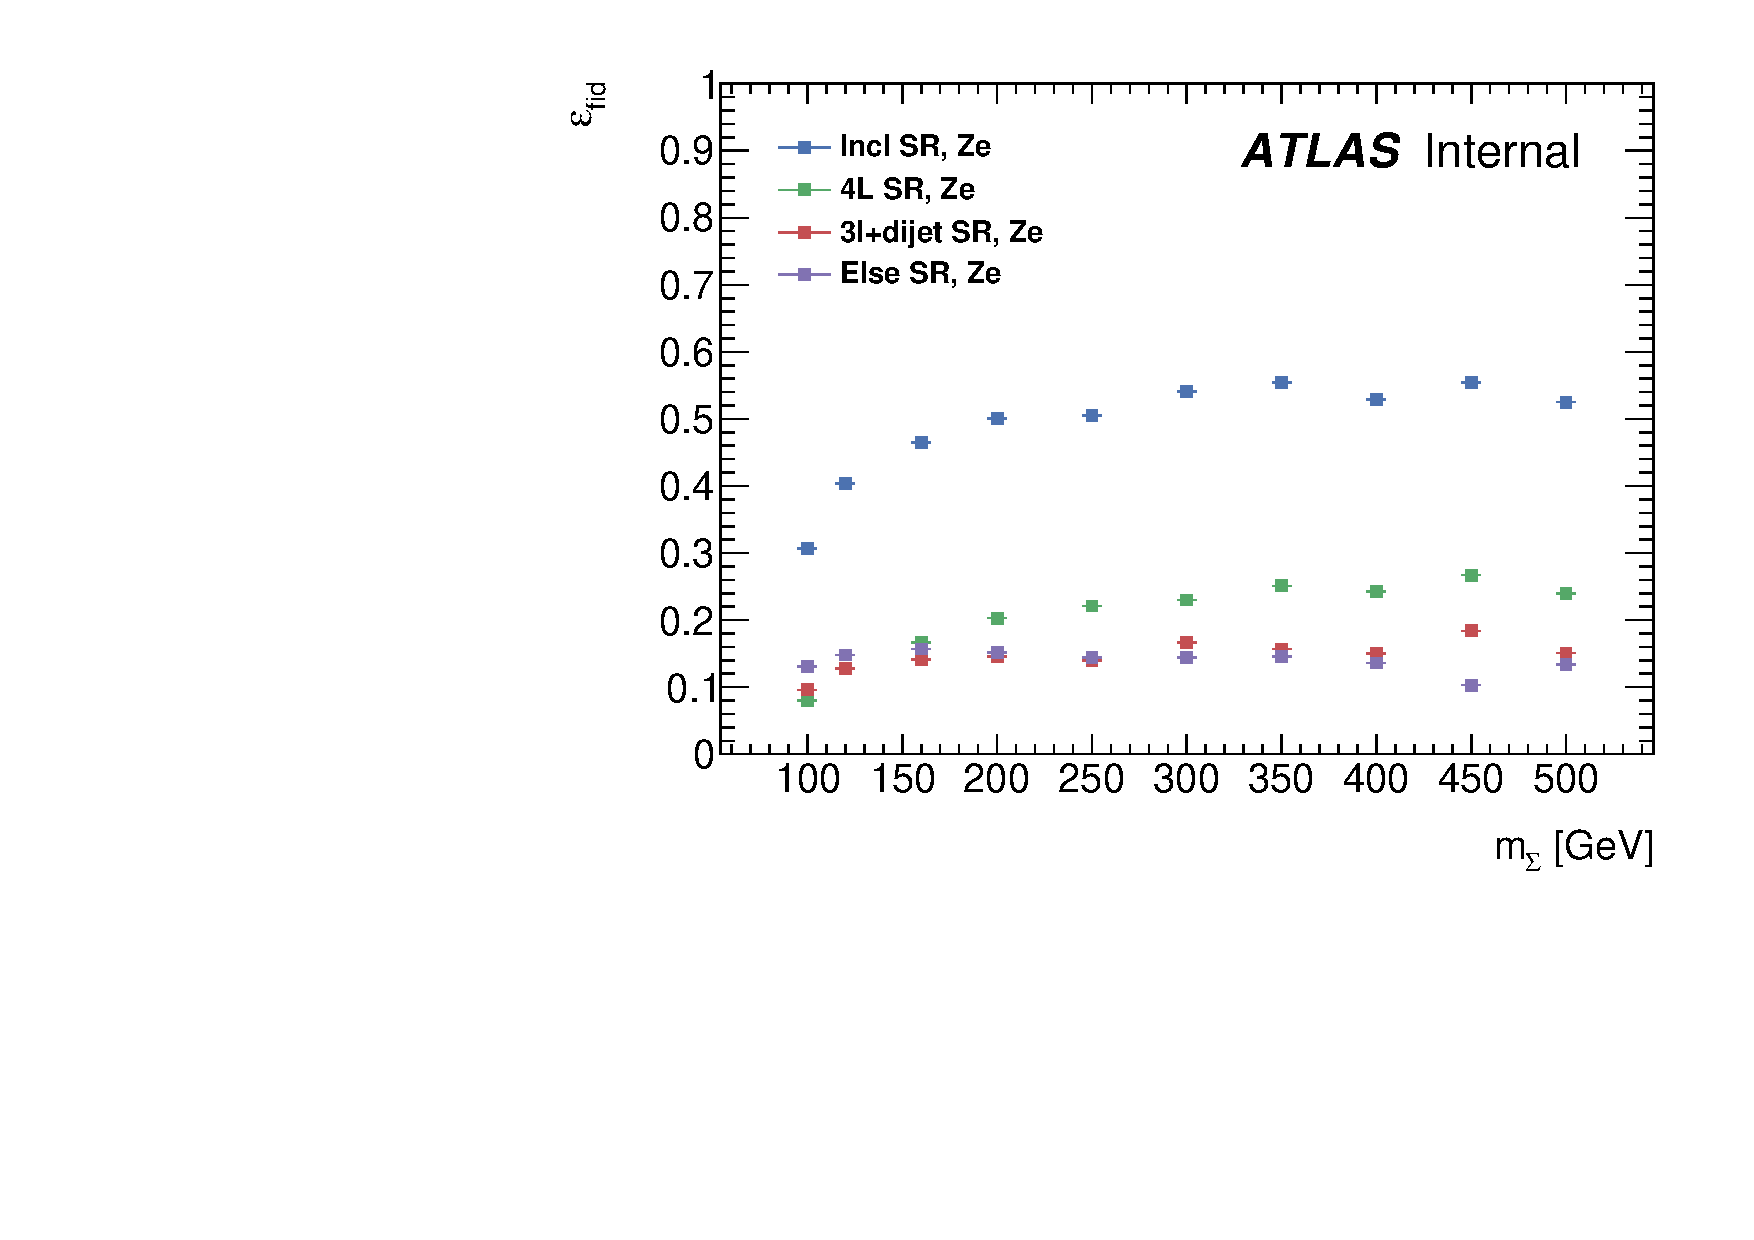
\includegraphics{figures/ch6-resonance/c_eff_fid_Ze_Seesaw}}
	}
	\subfloat[ $Z+e$, vector-like leptons] {
		\resizebox{0.4\textwidth}{!}{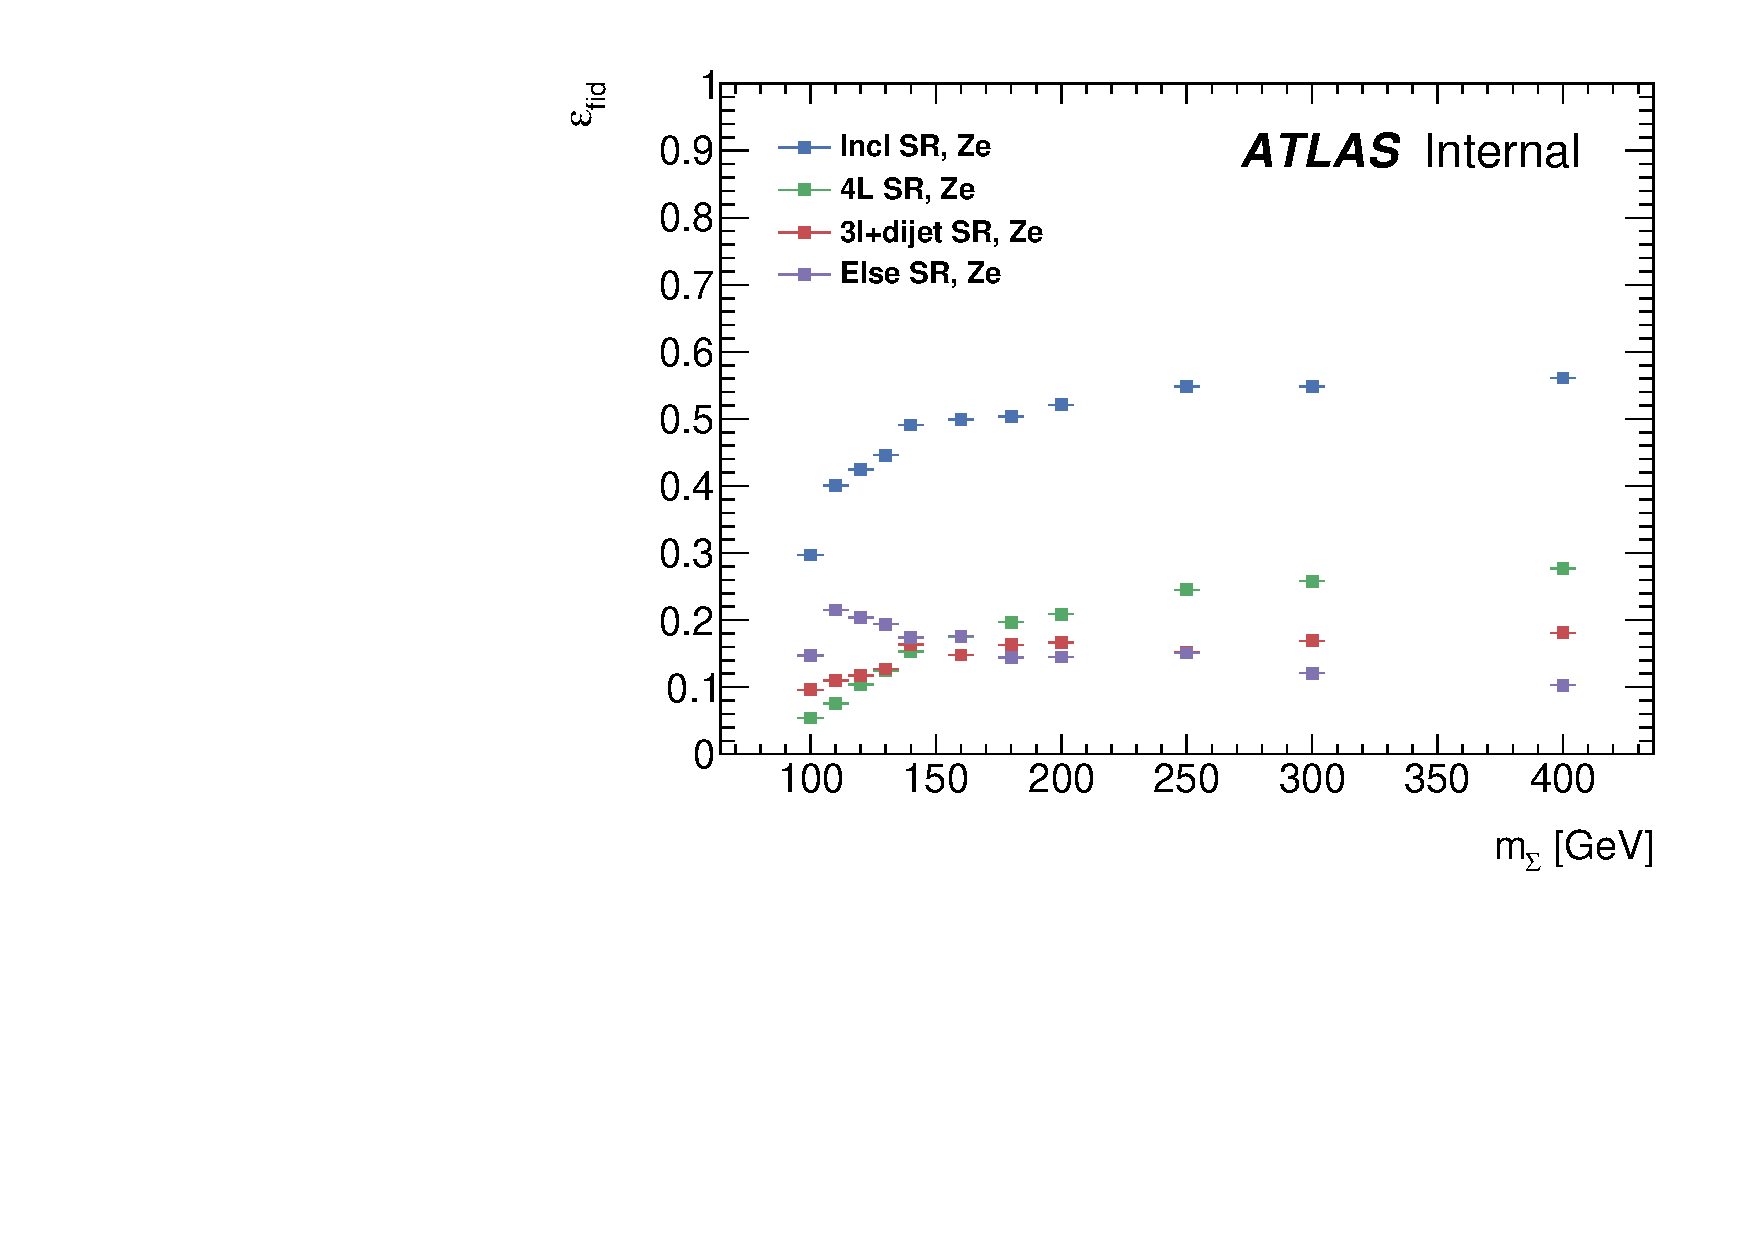
\includegraphics{figures/ch6-resonance/c_eff_fid_Ze_VLL}}
	} \\
	\subfloat[ $Z+\mu$, seesaw] {
		\resizebox{0.4\textwidth}{!}{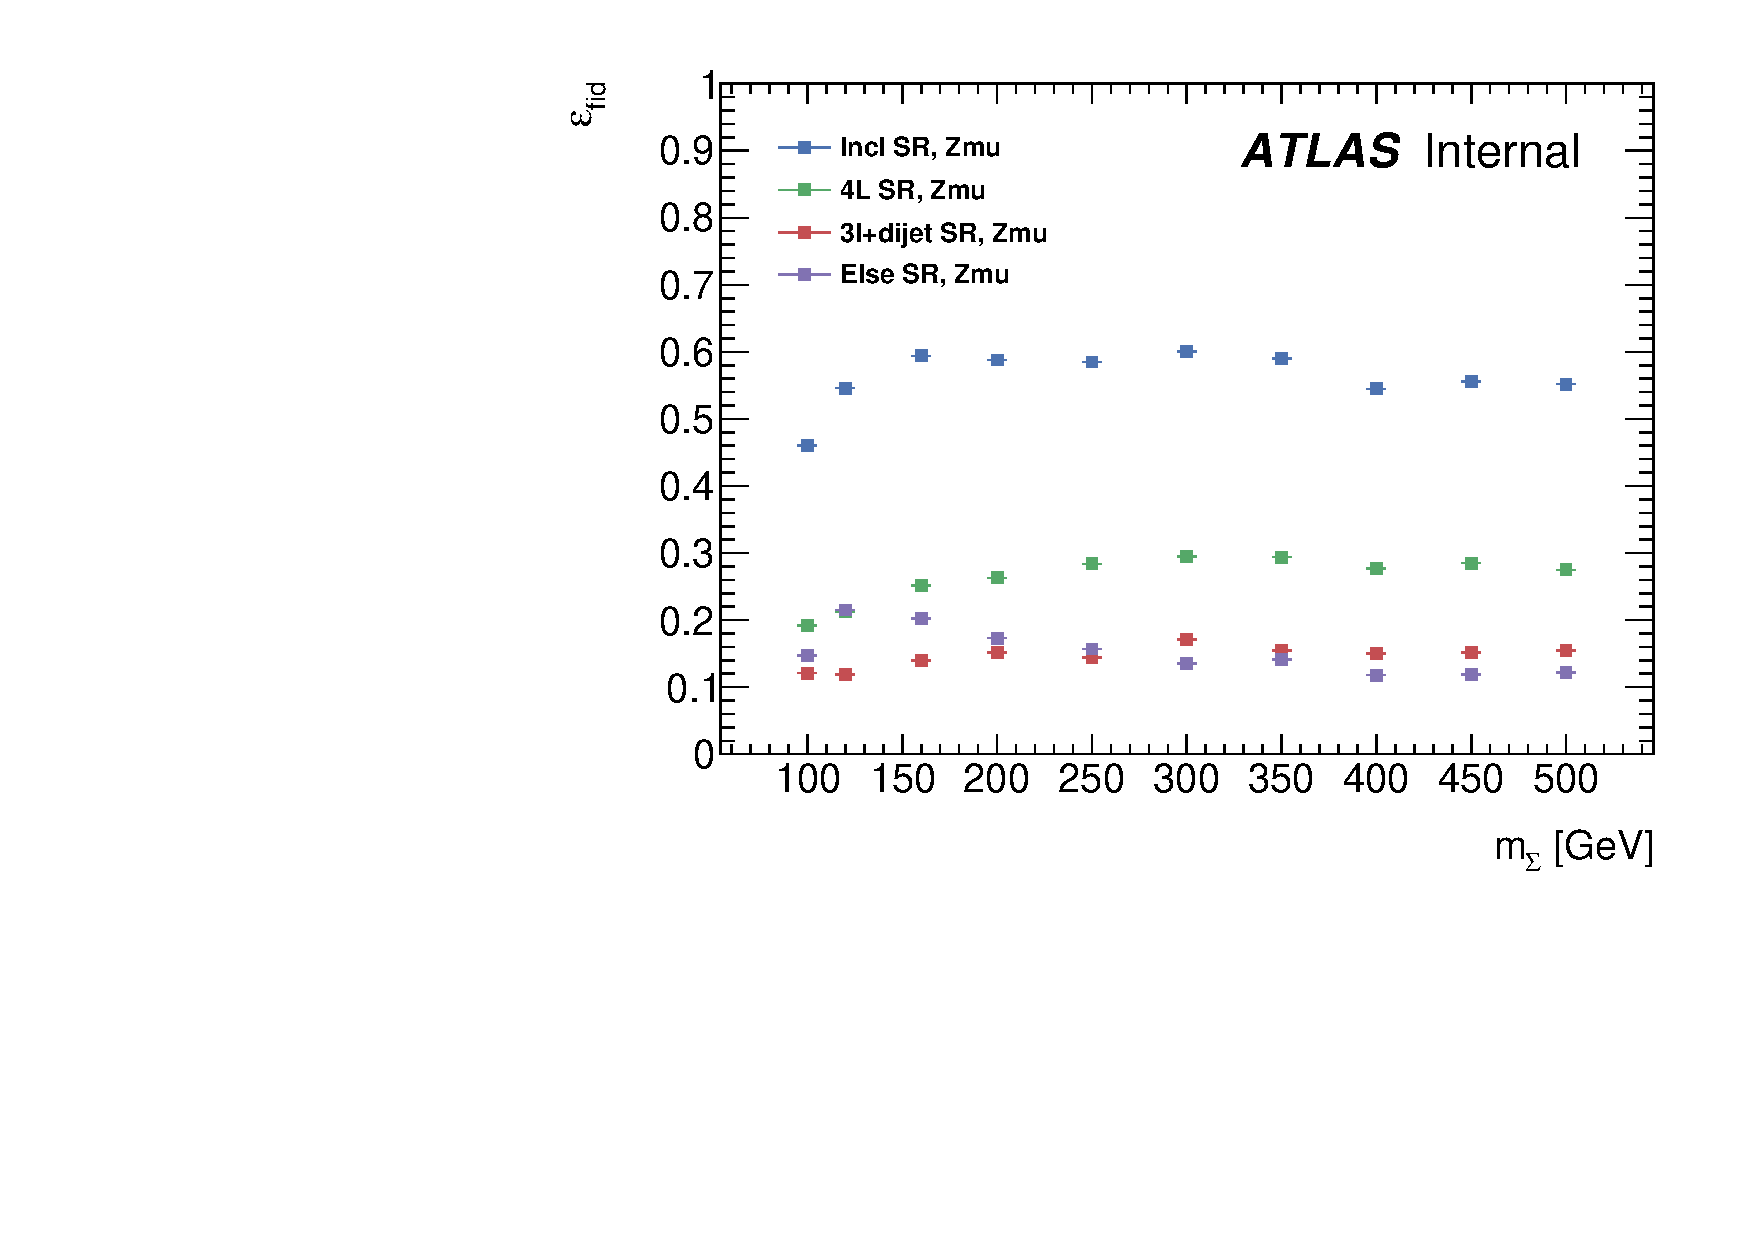
\includegraphics{figures/ch6-resonance/c_eff_fid_Zmu_Seesaw}}
	}
	\subfloat[ $Z+\mu$, vector-like leptons] {
		\resizebox{0.4\textwidth}{!}{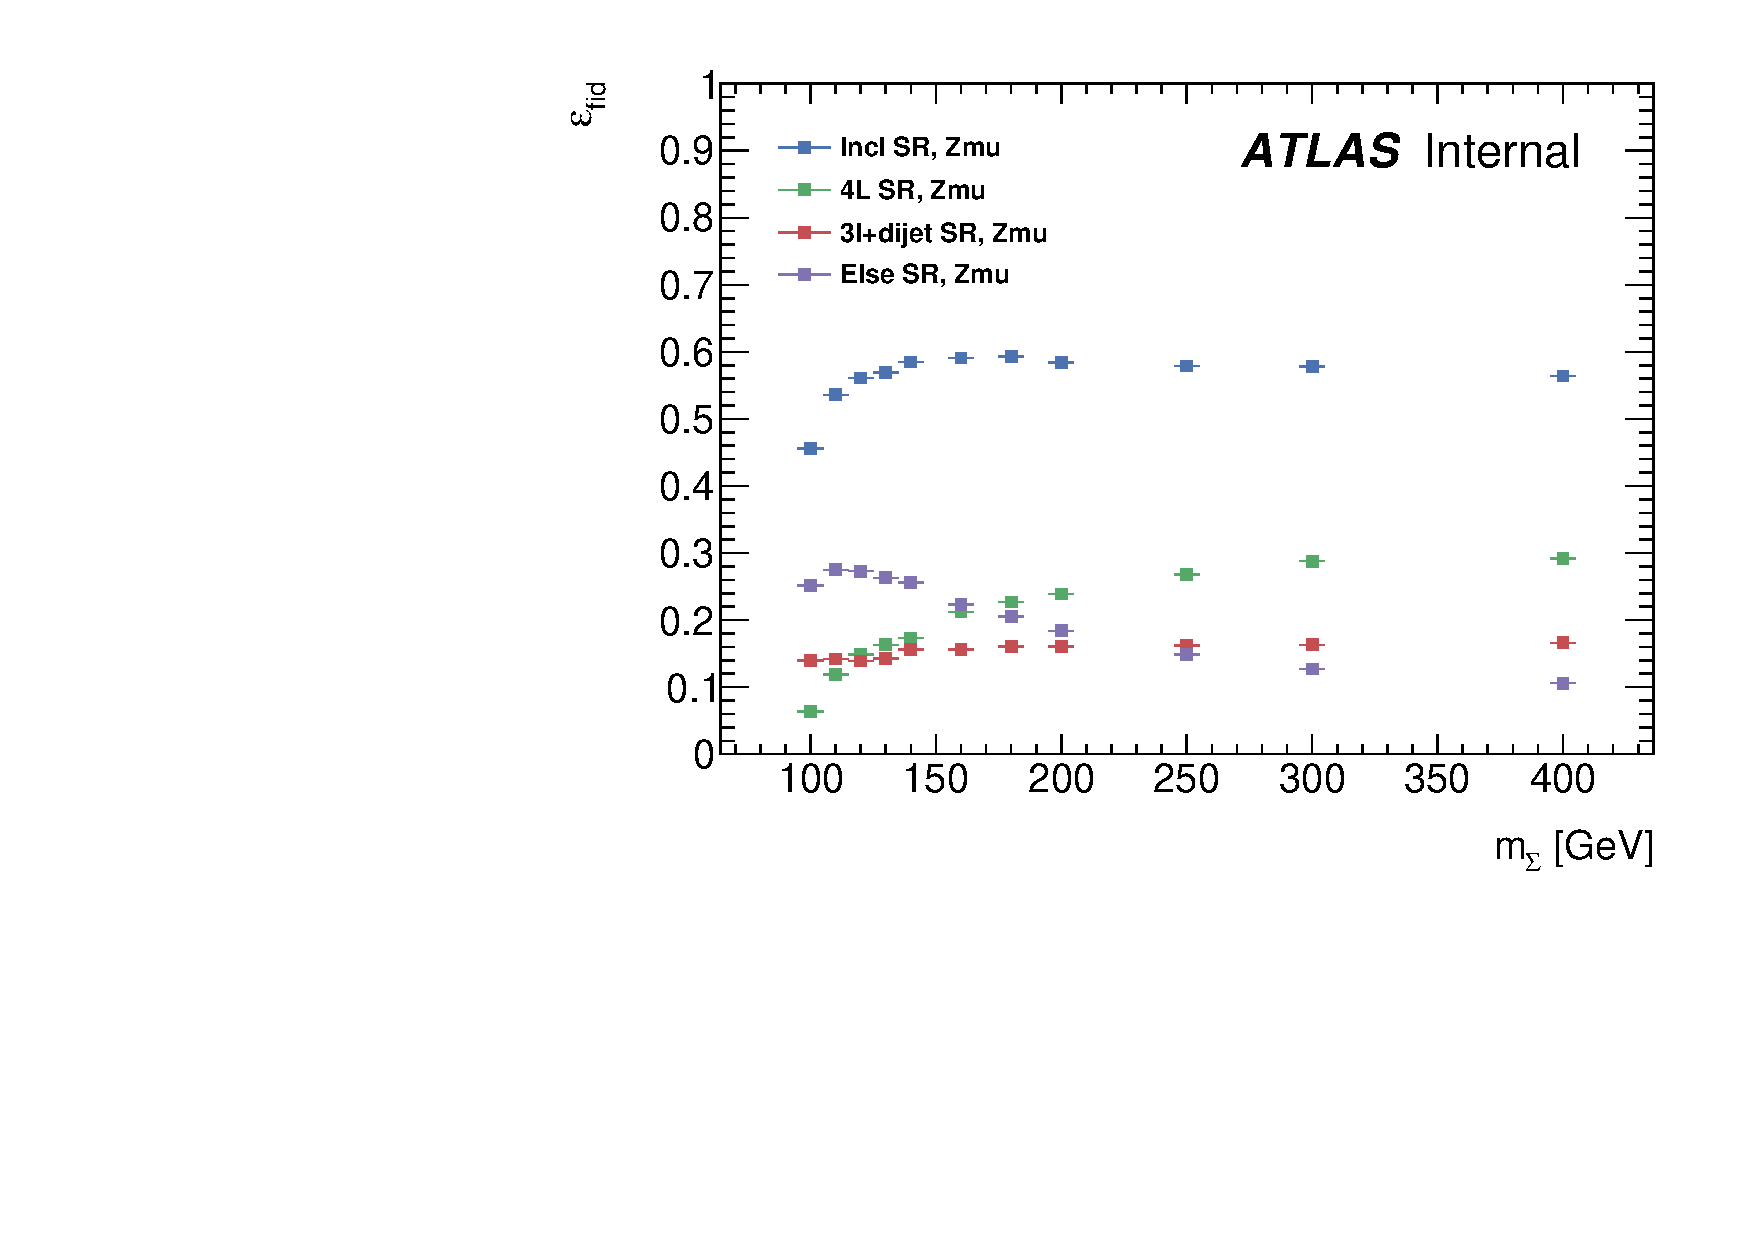
\includegraphics{figures/ch6-resonance/c_eff_fid_Zmu_VLL}}
	}
	\caption{Efficiencies of cuts defining each signal region on fiducial $Z(ll)l$ events at each simulated mass point. For the $Z+e$ signal regions, the branching fraction is set to be $BR(\Sigma\rightarrow X+e/\nu_{e})=100\%$; similarly, for the $Z+\mu$ signal regions, the branching fraction is set to be $BR(\Sigma\rightarrow X+\mu/\nu_{\mu})=100\%$.}
	\label{fig:fiducial-efficiencies-vs-mass}
\end{figure}




\section{Background Estimation}
The backgrounds to the trilepton resonance search are similar to those for the model-independent search described in section~\ref{sec:model-independent-background-estimation}. In the \fourl signal regions, $ZZ$ production is dominant. In the $\threeljj$ and $\threelo$ signal regions, $WZ$ production is dominant, with smaller contributions from $ZZ$ where one lepton is not selected, $\ttbarV$, and reducible backgrounds. 

The prompt backgrounds are estimated using Monte Carlo simulation. The samples are detailed below in section~\ref{sec:resonance-background-MC-samples}. The reducible $Z+\gamma$ backgrounds are also estimated using simulation. The remaining reducible backgrounds are estimated using the same fake factor method as described in section~\ref{sec:model-independent-fake-factor-method}. 

\subsection{Background Monte Carlo Samples}\label{sec:resonance-background-MC-samples}

\begin{table}
  \centering
  \caption{Summary of the \textcolor{black}{primary} signal and background MC samples used in this analysis. The generator, parton shower and hadronization, PDF, underlying event tune, and the order of the cross-section calculation are shown for each sample.}
  \begin{tabular}{|c|c|c|c|c|c|}
    \hline
    Process & Generator & Parton shower and hadr. & PDF set & UE tune & Cross section \\
    \hline
    VLL & \madgraph\ 4.5.2 & \pythia\ 8 & CTEQ6L1 & AU2	&	LO 	\\
    Seesaw & \madgraph\ 5.2.2.1 & \pythia\ 8 & CTEQ6L1 & AU2	&	LO 	\\
    $WZ$ & \sherpa 1.4.3 & \sherpa & CT10 & \sherpa 	&	NLO\\
    $ZZ$ & \sherpa 1.4.5 & \sherpa & CT10 & \sherpa 	&	NLO\\
   % $\ttbar+W/Z$ & \alpgen\ 2.13 ~\cite{alpgen}  & \herwig\ 6.520~\cite{herwig}   & CTEQ6L1 & \jimmy\ 4.31~\cite{jimmy} 	&	\\
    $\ttbar+W/Z$ & \madgraph\ 5.1.3.33  & \pythia\ 6.426   & {CTEQ6L1} & AUET2B 	&	NLO\\
    $VVV^{(*)}$ & \madgraph\ 5.1.3.33 & \pythia\ 6.426 & {CTEQ6L1}  & AUET2B 	& 	LO	\\
    $Z+\gamma$ & \sherpa  & \sherpa & CT10 & \sherpa 	&	LO 	\\
    \hline
  \end{tabular}
  \label{table:resonance-background-samples}
\end{table}


The Monte Carlo samples used to model the background processes are summarized in table~\ref{table:resonance-background-samples}. For all samples, the response of the ATLAS detector is modelled using the \geant~toolkit~\cite{geant,atlassimulation}. Pileup interactions in the same or nearby bunch crossings are modeled by overlaying minimum-bias interactions modelled with \pythia~6.425 onto the hard-scatter event. The simulated events are assigned weights to reprocude the distribution of the average number of $pp$ interactions per crossing observed in data. 

The dominant backgrounds due to Standard Model $WZ$ ($ZZ$) production are modelled using the \sherpa~\cite{sherpa} MC generator version 1.4.3 (1.4.5), using the internal showering algorithm~\cite{Hoeche:2009rj,Gleisberg:2008fv,Schumann:2007mg}a nd  the CT10~\cite{ct10} PDF set. The samples are normalized using cross sections calculated at next-to-leading-order (NLO) in QCD with \vbfnlo-2.6.2~\cite{vbfnlo}.  The generation includes up to three additional parton emissions in the matrix element. Samples of simulated events based on the NLO generator \powheg~\cite{powheg} are used to derive systematic uncertainties on the shapes of distributions predicted by \sherpa. The diboson samples are showered with \pythia~8, and use the CT10 PDF set and AU2 underlying event tune.

Drell--Yan production in association with a photon that converts in the detector, denoted $Z+\gamma$, is modelled using \sherpa~1.4.1, also using the CT10 PDF set and including up to three additional parton emissions in the matrix element. Production of top-quark pairs in association with a $W$ or $Z$ boson ($\ttbarV$) and triboson production ($VVV^{(*)}$) are modelled using \madgraph~5.1.3.33, with \pythia~6.426 for the parton shower and hadronization, AUET2B underlying event tune~\cite{AUET2B}, and the CTEQ6L1 PDF set. The $\ttbarV$ processes are normalized to the corresponding NLO cross sections~\cite{Campbell:2012dh,Lazopoulos:2008de}, while the $Z+\gamma$ and $VVV^{(*)}$ processes are normalized to their LO cross sections from the respective generator.


\section{Systematic Uncertainties}\label{sec:resonance-systematic-uncertainties}
The signal predictions and background estimates are assigned systematic uncertainties from several sources. In approximate order of significance, these are:

\begin{itemize}
	\item \textbf{Diboson shape uncertainty}: A systematic uncertainty is assigned to the modeling of the diboson backgrounds by comparing \sherpa~to \powheg. \sherpa~is used as a central value, with uncertainty given by the symmetric difference between \sherpa~and \powheg. As described below in section~\ref{sec:fit-method}, the shapes for the 4L and Rest signal regions are taken from the inclusive signal region, so the corresponding uncertainties are derived only from the inclusive and 3L+dijet signal regions. The comparison for the $WZ$ background is shown in figure~\ref{fig:systematic-WZ-shape}. The implementation of this uncertainty in the fit-based limit section is discussed in more detail in section~\ref{sec:fit-limits-systematic-uncertainties}; briefly, the uncertainty is included as a gaussian-distributed nuisance parameter interpolating between the two fits estimated from the two generators.

	In the case of the $ZZ$ background, this procedure is complicated by the fact that the \powheg~sample is filtered to remove events with same-flavor, opposite-sign lepton pairs with $m_{l^+l^-}<4~\mbox{GeV}$ (mll4). In order to compare the samples in a common phase space, the mll4 filter is emulated on the \sherpa~sample by rejected events that contain a same-flavor, opposite-sign pair of truth leptons with status==3, with $m_{l^+l^-}<4~\mbox{GeV}$. \sherpa, ~\sherpa~with mll4 filter, and \powheg~are compared in figure~\ref{fig:ZZ-mll4}. The events from the \powheg~sample are weighted using the ratio of \sherpa~to \sherpa+mll4. The final comparison of background shapes is shown in figure~\ref{fig:systematic-ZZ-shape}.

	\begin{figure}[h]
		\centering
		\subfloat[ Inclusive SR, $Z+e$] {
			\resizebox{2.5in}{!}{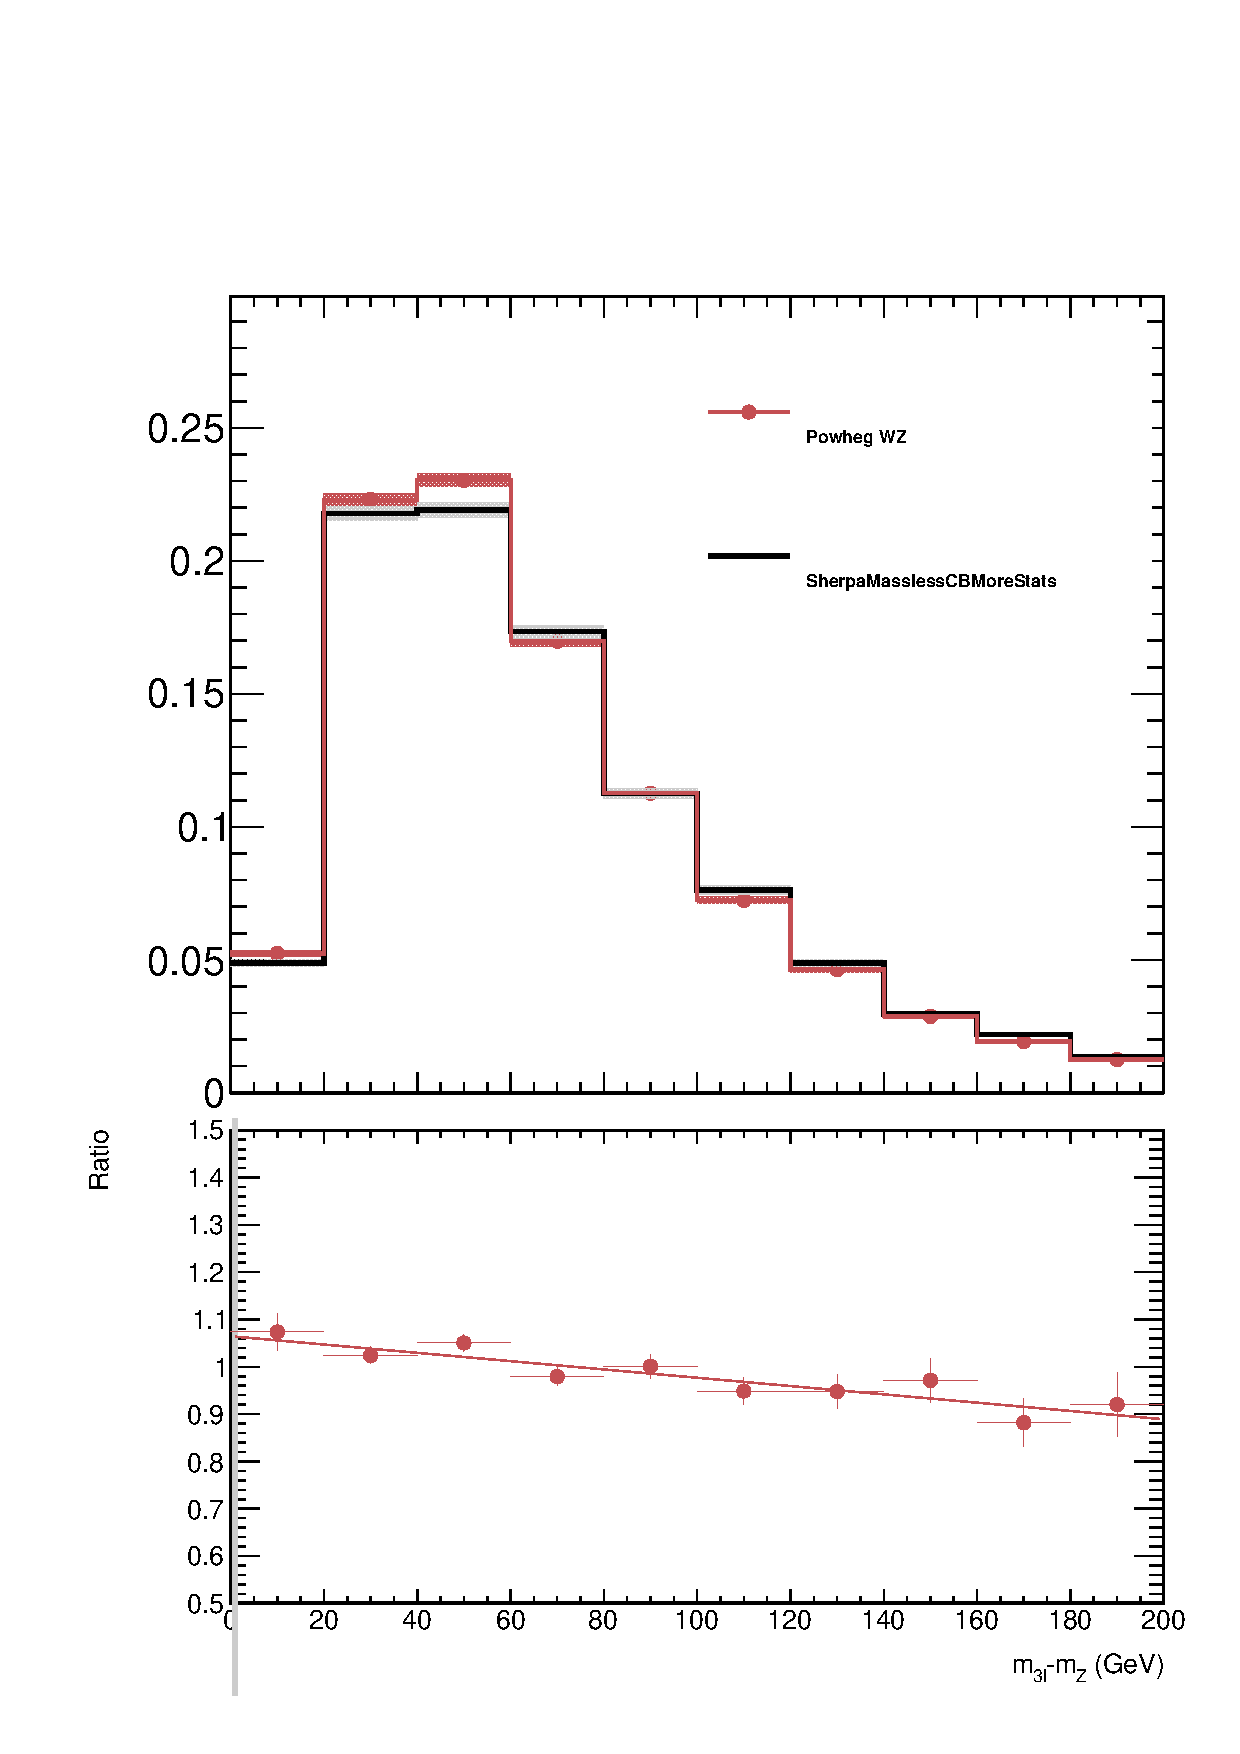
\includegraphics{figures/ch6-resonance/c_systematics_WZShape_Ze_InclusiveNoM3L_WZ.pdf}}
		}
		\subfloat[ ThreeLDijet SR, $Z+e$] {
			\resizebox{2.5in}{!}{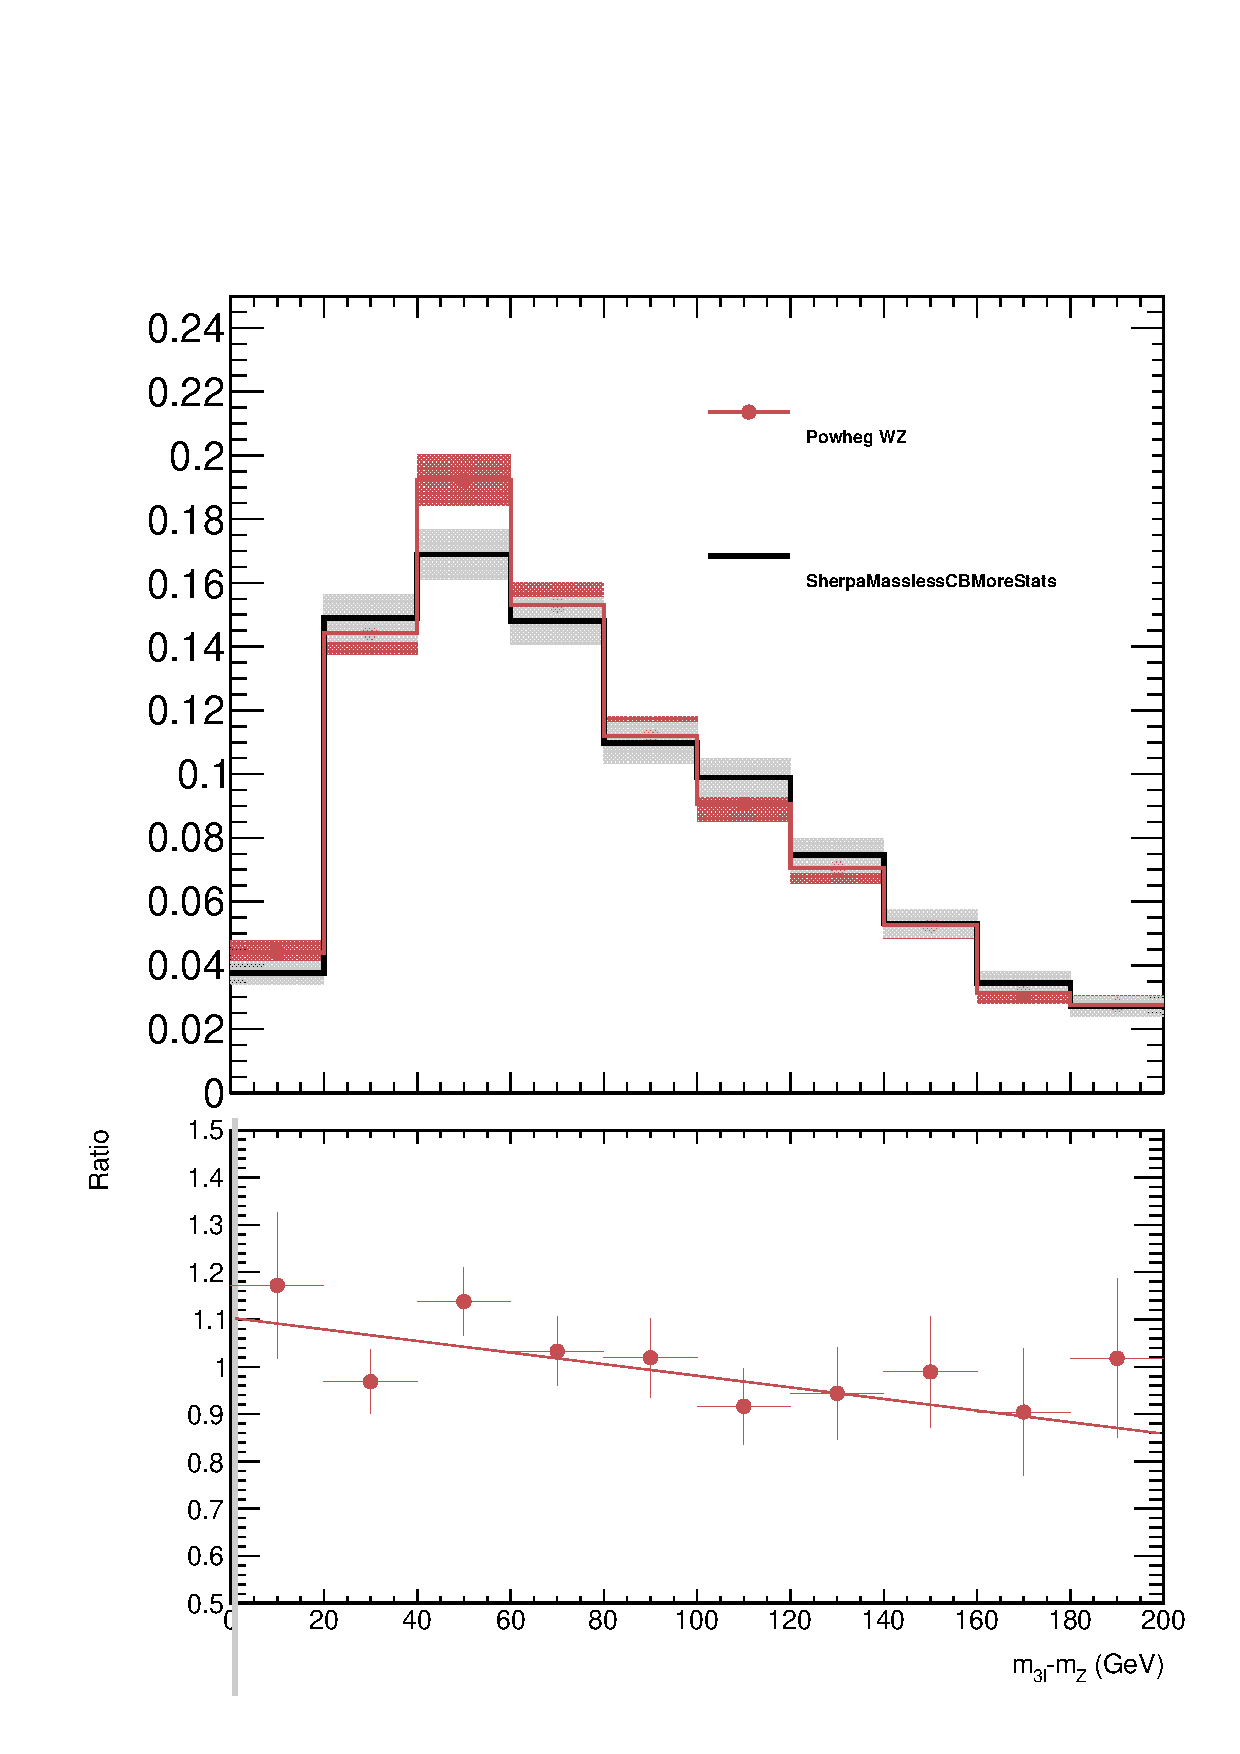
\includegraphics{figures/ch6-resonance/c_systematics_WZShape_Ze_ThreeLDijetNoM3L_WZ.pdf}}
		} \\
		\subfloat[ Inclusive SR, $Z+\mu$] {
			\resizebox{2.5in}{!}{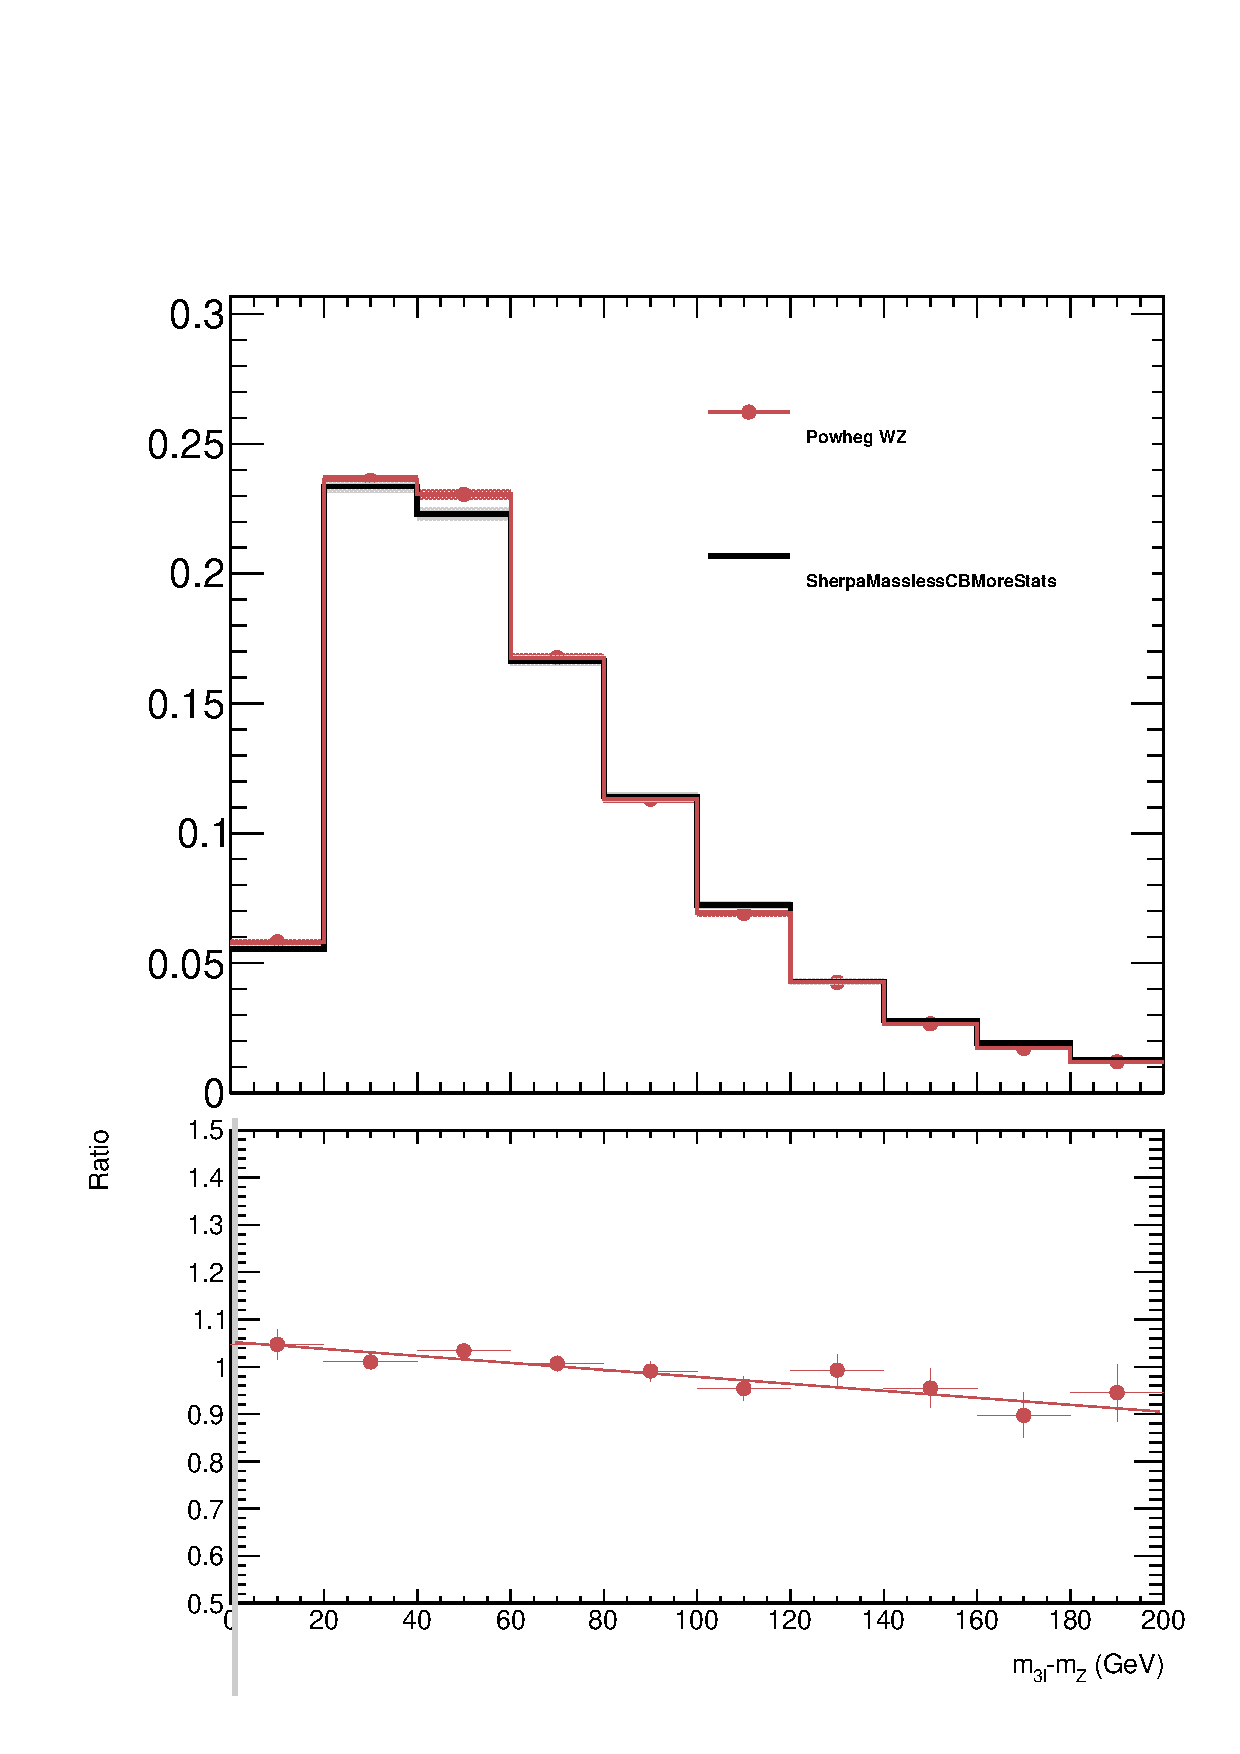
\includegraphics{figures/ch6-resonance/c_systematics_WZShape_Zmu_InclusiveNoM3L_WZ.pdf}}
		}
		\subfloat[ ThreeLDijet SR, $Z+\mu$] {
			\resizebox{2.5in}{!}{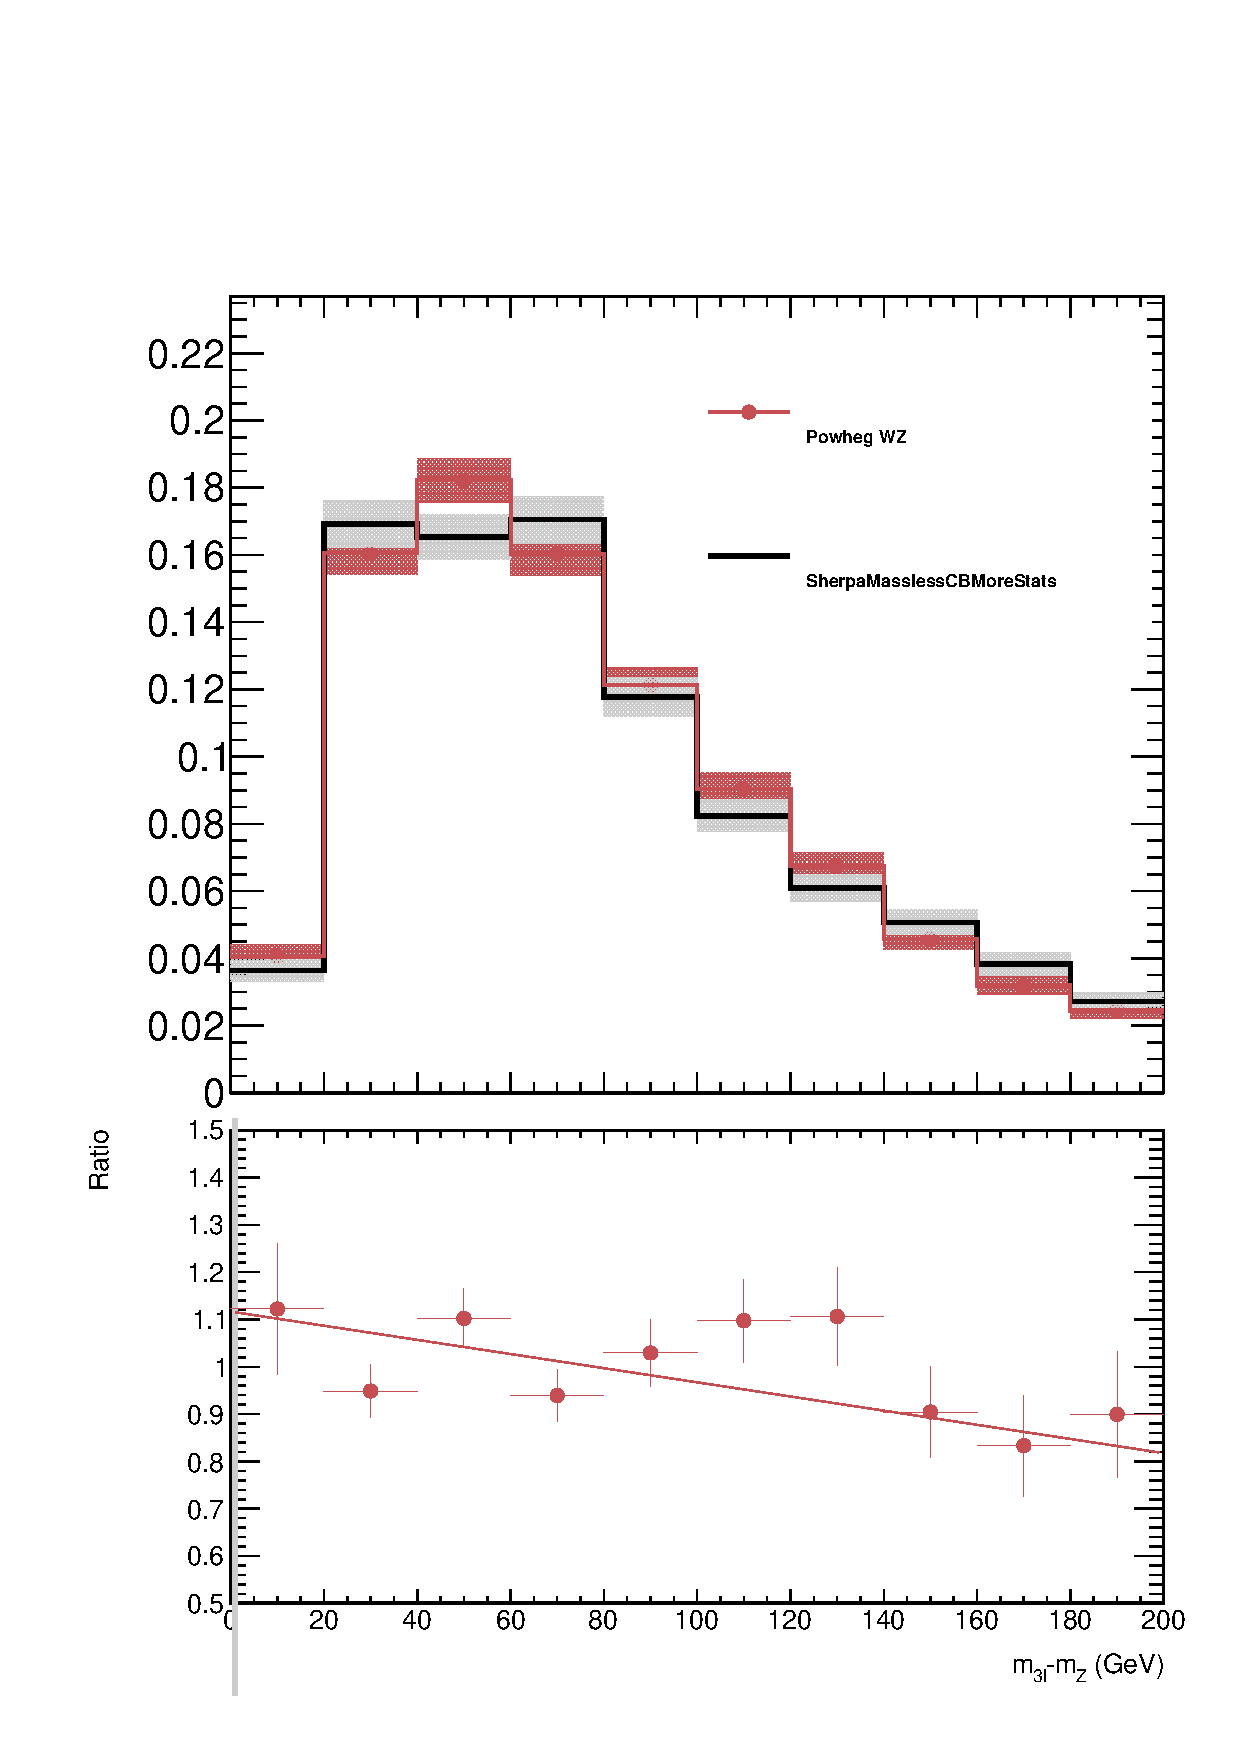
\includegraphics{figures/ch6-resonance/c_systematics_WZShape_Zmu_ThreeLDijetNoM3L_WZ.pdf}}
		}
		\caption{Comparison of the $\deltam$ distributions between \powheg~and \sherpa~for the $WZ$ backgrounds. The 4L signal region is omitted due to the negligible number of $WZ$ events with four leptons.}
		\label{fig:systematic-WZ-shape}
	\end{figure}

	\begin{figure}[h]
		\centering
		\subfloat[ Inclusive SR, $Z+e$] {
			\resizebox{2.5in}{!}{\includegraphics{figures/ch6-resonance/c_systematics_ZZShape_DeltaM_Ze_InclusiveNoM3L}}
		}
		\subfloat[ ThreeLDijet SR, $Z+e$] {
			\resizebox{2.5in}{!}{\includegraphics{figures/ch6-resonance/c_systematics_ZZShape_DeltaM_Ze_ThreeLDijetNoM3L}}
		} \\
		\subfloat[ Inclusive SR, $Z+\mu$] {
			\resizebox{2.5in}{!}{\includegraphics{figures/ch6-resonance/c_systematics_ZZShape_DeltaM_Zmu_InclusiveNoM3L}}
		}
		\subfloat[ ThreeLDijet SR, $Z+\mu$] {
			\resizebox{2.5in}{!}{\includegraphics{figures/ch6-resonance/c_systematics_ZZShape_DeltaM_Zmu_ThreeLDijetNoM3L}}
		}
		\caption{Comparison of \sherpa, \sherpa~with mll4 filter, and \powheg.}
		\label{fig:ZZ-mll4}
	\end{figure}
	

	\begin{figure}[h]
		\centering
		\subfloat[ Inclusive SR, $Z+e$] {
			\resizebox{2.5in}{!}{\includegraphics{figures/ch6-resonance/c_systematics_ZZShapeSyst_Ze_InclusiveNoM3L.pdf}}
		}
		\subfloat[ ThreeLDijet SR, $Z+e$] {
			\resizebox{2.5in}{!}{\includegraphics{figures/ch6-resonance/c_systematics_ZZShapeSyst_Ze_ThreeLDijetNoM3L.pdf}}
		} \\
		\subfloat[ Inclusive SR, $Z+\mu$] {
			\resizebox{2.5in}{!}{\includegraphics{figures/ch6-resonance/c_systematics_ZZShapeSyst_Zmu_InclusiveNoM3L.pdf}}
		}
		\subfloat[ ThreeLDijet SR, $Z+\mu$] {
			\resizebox{2.5in}{!}{\includegraphics{figures/ch6-resonance/c_systematics_ZZShapeSyst_Zmu_ThreeLDijetNoM3L.pdf}}
		}
		\caption{Comparison of the $\deltam$ distributions between \powheg~and \sherpa~for the $ZZ$ backgrounds. The \powheg~events are weighted to account for the mll4 filter.}
		\label{fig:systematic-ZZ-shape}
	\end{figure}
	

	\item \textbf{Monte Carlo statistics and Fit Parameter Uncertainties}: as described below in section~\ref{sec:fit-method}, the limit setting is performed using fits with analytical functions to the Monte Carlo background predictions. Hence the uncertainty due to the finite statistics of the background samples is in represented in the uncertainties on the fit parameters, returned by the fitting code. This uncertainty is discussed in more detail in section~\ref{sec:fit-limits-systematic-uncertainties}.


	\item \textbf{Monte Carlo sample normalizations}: The Monte Carlo samples used for the irreducible background prediction are normalized to the measured luminosity of the data using theoretical cross sections. The uncertainty on the luminosity is $2.8\%$~\cite{luminosity}. The uncertainties on the cross sections for $WZ$, $ZZ$, and $t\overline{t}+V$ are listed in table~\ref{table:mc-cross-section-uncertainties}. The $WZ$ and $ZZ$ uncertainties are taken from \cite{DeViveiros:1670929}, and are based off a comparison of \sherpa with \vbfnlo. A cross section uncertainty is not assigned to the $Z+\gamma$ backgrounds; instead, as described next, a large uncertainty is assigned due to applying scale factors to correct the simulated rate of photon conversions. Similarly, an uncertainty is not assigned for the $VVV^{(*)}$ cross section, due to its small contribution to the signal regions. 

	In the fit-based limit setting procedure, the uncertainty is implemented as a constraint on the normalization of the corresponding sample: the normalizations of the dominant diboson samples are allowed to float within the quadrature sum of all the normalization uncertainties. The normalizations of the small $t\overline{t}+V$ and $VVV^{(*)}$ backgrounds are fixed due to their comparatively small magnitude, which the fit is unable to resolve. 

	\begin{table}[h]
		\centering
		\begin{tabular}{ccc}
			Process & Cross Section Uncertainty & Reference \\
			\hline
			$WZ$ & $7.6\%$ & \cite{DeViveiros:1670929}\\
			$ZZ$ & $4.3\%$ & \cite{DeViveiros:1670929} \\
			$t\overline{t}+V$ & $22\%$ & \cite{ttV} \\
		\end{tabular}	
		\caption{Cross sections and uncertainties for the Monte Carlo samples used for irreducible background estimation.}
		\label{table:mc-cross-section-uncertainties}
	\end{table}

	\item \textbf{Charge flip scale factors}: The rate of trilepton events due to $Z+\gamma$, where the photon converts asymmetrically and is reconstructed as an electron, is observed to be overestimated in Monte Carlo. Scale factors are applied following the charge flip likelihood estimation method from the same-sign dilepton analysis~\cite{DeViveiros:1670929}, and an uncertainty of $30\%$ is assigned to this background sample.

	\item \textbf{Fake factor method}: The systematic uncertainty on the fake factors is described in sections~\ref{sec:electron-fake-factors} and \ref{sec:muon-fake-factors}. They range from $20\%$-$30\%$ for electrons and $25\%$-$50\%$ for muons. 

	\item \textbf{Luminosity}: The uncertainty on the integrated luminosity in 2012 is $2.8\%$. 

	\item \textbf{Lepton scale factors}: Scale factors are applied to equalize the lepton trigger, reconstruction, and identification efficiencies between data and simulation. The corrections are implemented with official performance group tools: 

	\texttt{MuonEfficiencyCorrections}~\cite{MuonEfficiencyScaleFactors} and 

	\texttt{TElectronEfficiencyCorrectionTool}~\cite{ElectronEfficiencyScaleFactors}. 

	Systematic uncertainties on the scale factors are applied according to the official recommendations. 

	\item \textbf{Electron energy corrections}: To improve agreement in electron energy between data and simulation, the energy is scaled in data and smeared in Monte Carlo according to the recommendations at~\cite{ElectronEnergyCorrectionsGEO20,ElectronEnergyCorrectionsGEO21}. The corrections and corresponding systematic uncertainties are provided by the \texttt{ElectronPhotonFourMomentumCorrection} package. 

	\item \textbf{Muon mommentum corrections}: The muon momenta are smeared in simulation according to the recommendations at~\cite{MuonMomentumCorrections}. The corrections are derived by ``comparing the reconstructed muon momentum in experimental and simulated data,'' using $J/\psi$ and $Z$ decays. 

	\item \textbf{Jet energy scale and resolution}: Systematic uncertainties on the jet energy scale and resolution are applied following the recommendations from the Jet/ETMiss group~\cite{JetEtmissRecommendations2012}, and are taken from the package \texttt{JetUncertainties~00-08-07}. The jet energy uncertainties have a small impact on this analysis, only affecting the normalization in the 3L+dijet signal region when the dijet mass is pushed in or out of the window $m_{W}-20~\mbox{GeV}<m_{jj}<m_{h}+25~\mbox{GeV}$. 
\end{itemize}

Figures~\ref{fig:systematics-summary-Ze} and \ref{fig:systematics-summary-Zmu} show the fractional uncertainty due to each source of uncertainty in $20~\mbox{GeV}$ bins for each signal region, as well as the total systematic uncertainty and expected statistical uncertainty. Note that the uncertainties shown are bin-by-bin uncertainties on the Monte Carlo predictions, and do not necessarily correspond to the final uncertainty after fitting the background shapes; for example, after fitting, the Monte Carlo statistical uncertainties are contained in the uncertainties on the fit parameters. Further, the Monte Carlo statistical uncertainties are overrepresented, as they are also contained in the $WZ$/$ZZ$ shape uncertainties derived from the comparison of two statistically independent samples. Finally, due to the fact that the shapes for the 4L and 3L+dijet signal regions are taken from the inclusive signal region, the shape uncertainties derived in these categories are not used in the analysis.

The impact of each uncertainty in each signal region, in terms of fractional uncertainty on the total normalization, is shown for background in figure~\ref{table:systematics-summary}, and some example signal points in figures~\ref{table:systematics-impact-summary-seesaw-160}--\ref{table:systematics-impact-summary-seesaw-500}. The complete set of tables of signal systematics is in appendix~\ref{appx:signal-uncertainties}.


\begin{figure}[p]
	\centering
	\subfloat[ Inclusive SR, $Z+e$] {
		\resizebox{0.48\textwidth}{!}{\includegraphics{figures/ch6-resonance/c_systematics_DeltaM_Ze_InclusiveNoM3L_300GeV}}
	}
	\subfloat[ 4L SR, $Z+e$] {
		\resizebox{0.48\textwidth}{!}{\includegraphics{figures/ch6-resonance/c_systematics_DeltaM_Ze_FourLNoM3L_300GeV}}
	} \\
	\subfloat[ 3L+dijet SR, $Z+e$] {
		\resizebox{0.48\textwidth}{!}{\includegraphics{figures/ch6-resonance/c_systematics_DeltaM_Ze_ThreeLDijetNoM3L_300GeV}}
	}
	\subfloat[ Rest SR, $Z+e$] {
		\resizebox{0.48\textwidth}{!}{\includegraphics{figures/ch6-resonance/c_systematics_DeltaM_Ze_ElseNoM3L_300GeV}}
	}
	\caption{Systematics summary plots for each signal region in the $Z+e$ flavor channel. The contribution from each source of systematic uncertainty is shown in $20~\mbox{GeV}$ bins, along with the total systematic uncertainty and the expected statistical uncertainty. Note that these uncertainties reflect bin-by-bin uncertainties on the Monte Carlo predictions, and do not necessarily correspond to the final uncertainty after fitting the background shapes.}
	\label{fig:systematics-summary-Ze}
\end{figure}

\begin{figure}[p]
	\centering
	\subfloat[ Inclusive SR, $Z+e$] {
		\resizebox{0.48\textwidth}{!}{\includegraphics{figures/ch6-resonance/c_systematics_DeltaM_Zmu_InclusiveNoM3L_300GeV}}
	}
	\subfloat[ 4L SR, $Z+e$] {
		\resizebox{0.48\textwidth}{!}{\includegraphics{figures/ch6-resonance/c_systematics_DeltaM_Zmu_FourLNoM3L_300GeV}}
	} \\
	\subfloat[ 3L+dijet SR, $Z+e$] {
		\resizebox{0.48\textwidth}{!}{\includegraphics{figures/ch6-resonance/c_systematics_DeltaM_Zmu_ThreeLDijetNoM3L_300GeV}}
	}
	\subfloat[ Rest SR, $Z+e$] {
		\resizebox{0.48\textwidth}{!}{\includegraphics{figures/ch6-resonance/c_systematics_DeltaM_Zmu_ElseNoM3L_300GeV}}
	}
	\caption{Systematics summary plots for each signal region in the $Z+\mu$ flavor channel. The contribution from each source of systematic uncertainty is shown in $20~\mbox{GeV}$ bins, along with the total systematic uncertainty and the expected statistical uncertainty. Note that these uncertainties reflect bin-by-bin uncertainties on the Monte Carlo predictions, and do not necessarily correspond to the final uncertainty after fitting the background shapes.}
	\label{fig:systematics-summary-Zmu}
\end{figure}


\begin{table}[htbp]
  \renewcommand{\arraystretch}{1.5}
  \centering
  \begin{tabular}{|c|c|c|c|c||c|c|c|c|}
    \hline
     & \multicolumn{4}{c||}{$Z+e$} & \multicolumn{4}{c|}{$Z+\mu$} \\
    \hline
     &  Total & $4l$ SR & $3l+jj$ SR  & $3l$-only SR  & Total & $4l$ SR & $3l+jj$ SR  & $3l$-only SR  \\
    \hline
    $\sigma_{ZZ}$ & $0.9$  & $3.9$  & $0.9$  & $0.8$  & $0.7$  & $3.8$  & $0.4$  & $0.6$ \\
    $\sigma_{WZ}$ & $4.9$  & $0.1$  & $4.6$  & $5.1$  & $5.3$  & $-$  & $4.9$  & $5.6$  \\
    $\sigma_{ttV}$  & $0.4$  & $1.5$  & $2.9$  & $0.1$  & $0.4$  & $0.9$ & $2.9$  & $0.1$  \\
    Luminosity  & $2.6$ & $2.8$  & $2.7$  & $2.6$  & $2.5$  & $2.6$  & $2.4$  & $2.5$  \\
    $\gamma$ conv. SFs  & $2.0$  & $-$ & $1.2$  & $2.1$  & $-$ & $-$ & $-$ & $-$ \\
    $\ell$ efficiency & $1.6$  & $1.8$  & $1.6$  & $1.6$  & $0.9$  & $0.9$  & $1.0$  & $0.9$  \\
    $e$ reducible SFs  & $1.7$  & $-$ & $0.5$  & $1.9$ & $0.1$ & $0.9$  & $0.1$  & $0.1$  \\
    $\mu$ reducible SFs  &  $0.3$ & $-$ & $0.3$ & $0.3$ & $3.4$ & $0.6$ & $4.3$ & $3.5$  \\
    JES/JER & $0.1$  & $_{-0.0}^{+0.2}$  & $3.3$  & $0.4$  & $0.1$  & $0.2$  & $3.2$  & $0.5$  \\
    LES/LER & $0.6$ & $_{-0.3}^{+1.0}$  & $_{-1.2}^{+0.3}$  & $_{-0.4}^{+0.7}$  & $0.1$  & $0.1$  & $0.2$  & $0.1$  \\
    MC Statistics & $2.4$ & $5.0$ & $4.3$ & $2.6$ & $1.2$ & $3.5$ & $2.8$ & $1.2$ \\
    \hline
    \hline
    Total & $6.9$ & $7.4$ & $8.4$ & $7.1$ & $7.0$ & $6.0$ & $8.7$ & $7.2$ \\
    % Old: wrong muon FFs. 
    % Total & $_{-7.21}^{+7.55}$  & $_{-5.29}^{+5.38}$  & $_{-7.79}^{+8.59}$  & $_{-7.47}^{+7.87}$  & $_{-6.06}^{+6.06}$  & $_{-4.83}^{+4.83}$  & $_{-6.65}^{+7.15}$  & $_{-6.26}^{+6.27}$  \\
    \hline
  \end{tabular}
  \caption{The impact of significant sources of uncertainty on the background prediction in each signal region, in terms of percent of the total background normalization.}
  \label{table:systematics-summary}
\end{table}

\begin{table}[htbp]
  \centering
  \begin{tabular}{|c|c|c|c|c||c|c|c|c|}
    \hline
     & \multicolumn{4}{|c||}{$Z+e$} & \multicolumn{4}{c|}{$Z+\mu$} \\
    \hline
     &  Incl SR & $4l$ SR & $3l+jj$ SR  & $3l$-only SR  & Incl SR & $4l$ SR & $3l+jj$ SR  & $3l$-only SR  \\
    \hline
    Luminosity  & $2.8$ & $2.8$ & $2.8$ & $2.8$ & $2.8$ & $2.8$ & $2.8$ & $2.8$ \\
    $l$ scale factors & $1.7$ & $1.7$ & $1.7$ & $1.6$ & $1.1$ & $1.1$ & $1.1$ & $1.0$ \\
    MC Statistics & $2.1$ & $4.5$ & $3.7$ & $3.0$ & $1.4$ & $2.7$ & $2.7$ & $2.2$ \\
    JES/JER & $0.0$ & $0.2$ & $3.6$ & $3.0$ & $0.2$ & $0.3$ & $3.0$ & $2.2$ \\
    LES/LER & $0.1$ & $0.4$ & $0.1$ & $0.1$ & $0.1$ & $0.2$ & $0.2$ & $0.2$ \\
    \hline
    \hline
    Total & $3.9$ & $5.6$ & $6.1$ & $5.3$ & $3.3$ & $4.0$ & $5.1$ & $4.3$ \\
    \hline
  \end{tabular}
  \caption{The impact of different sources of systematic uncertainty on the signal prediction for the type~III seesaw model with $m_{\Sigma}=160 \GeV$, in terms of percent of the total signal normalization.}
  \label{table:systematics-impact-summary-seesaw-160}
\end{table}

\begin{table}[htbp]
  \centering
  \begin{tabular}{|c|c|c|c|c||c|c|c|c|}
    \hline
     & \multicolumn{4}{|c||}{$Z+e$} & \multicolumn{4}{c|}{$Z+\mu$} \\
    \hline
     &  Incl SR & $4l$ SR & $3l+jj$ SR  & $3l$-only SR  & Incl SR & $4l$ SR & $3l+jj$ SR  & $3l$-only SR  \\
    \hline
    Luminosity  & $2.8$ & $2.8$ & $2.8$ & $2.8$ & $2.8$ & $2.8$ & $2.8$ & $2.8$ \\
    $l$ scale factors & $1.8$ & $1.7$ & $1.8$ & $1.9$ & $1.2$ & $1.2$ & $1.2$ & $1.2$ \\
    MC Statistics & $3.0$ & $5.7$ & $4.9$ & $4.7$ & $2.2$ & $3.7$ & $3.8$ & $3.6$ \\
    JES/JER & $0.1$ & $-$ & $1.6$ & $1.7$ & $0.2$ & $0.3$ & $2.0$ & $2.3$ \\
    LES/LER & $0.4$ & $0.1$ & $1.0$ & $0.4$ & $0.3$ & $0.0$ & $0.9$ & $0.3$ \\
    \hline
    \hline
    Total & $4.5$ & $6.5$ & $6.2$ & $6.0$ & $3.8$ & $4.8$ & $5.3$ & $5.3$ \\
    \hline
  \end{tabular}
  \caption{The impact of different sources of systematic uncertainty on the signal prediction for the type~III seesaw model with $m_{\Sigma}=300 \GeV$, in terms of percent of the total signal normalization.}
  \label{table:systematics-impact-summary-seesaw-300}
\end{table}

\begin{table}[htbp]
  \centering
  \begin{tabular}{|c|c|c|c|c||c|c|c|c|}
    \hline
     & \multicolumn{4}{|c||}{$Z+e$} & \multicolumn{4}{c|}{$Z+\mu$} \\
    \hline
     &  Incl SR & $4l$ SR & $3l+jj$ SR  & $3l$-only SR  & Incl SR & $4l$ SR & $3l+jj$ SR  & $3l$-only SR  \\
    \hline
    Luminosity  & $2.8$ & $2.8$ & $2.8$ & $2.8$ & $2.8$ & $2.8$ & $2.8$ & $2.8$ \\
    $l$ scale factors & $1.8$ & $1.8$ & $1.8$ & $2.0$ & $1.3$ & $1.4$ & $1.3$ & $1.3$ \\
    MC Statistics & $3.0$ & $5.5$ & $4.8$ & $4.8$ & $2.4$ & $4.0$ & $3.9$ & $4.1$ \\
    JES/JER & $-$ & $-$ & $1.7$ & $1.9$ & $0.3$ & $0.5$ & $1.8$ & $2.5$ \\
    LES/LER & $0.4$ & $0.5$ & $2.1$ & $1.7$ & $0.4$ & $1.6$ & $2.8$ & $2.2$ \\
    \hline
    \hline
    Total & $4.5$ & $6.4$ & $6.4$ & $6.4$ & $3.9$ & $5.4$ & $6.0$ & $6.1$ \\
    \hline
  \end{tabular}
  \caption{The impact of different sources of systematic uncertainty on the signal prediction for the type~III seesaw model with $m_{\Sigma}=500 \GeV$, in terms of percent of the total signal normalization.}
  \label{table:systematics-impact-summary-seesaw-500}
\end{table}


\section{Background Validation}\label{sec:resonance-background-validation}
For each flavor channel, four validation regions are defined to test the background predictions from the Monte Carlo simulation samples and the fake factor procedure. Each region starts from the set of events with three selected electrons or muons, two of which form an OSSF pair of leptons. 

The \underline{\textbf{high $\Delta R$}} region contains events with large separation between the $Z$ candidate momentum and the off-$Z$ lepton momentum, $\Delta R(Z,\ \ell_3)>3$. Events are also required to have exactly three leptons, and to satify $\deltam<200 \GeV - m_Z$, to limit signal contamination from hypotheses with larger $m_{\lpm}$ where the $Z$ and the off-$Z$ lepton are less collimated. The region has a similar background composition to the signal regions with three leptons, and tests the $WZ$, $ZZ$, and reducible background predictions.

The \underline{\textbf{$ZZ$}} region contains events with two OSSF lepton pairs with invariant mass within $10 \GeV$ of $m_Z$. The region tests the $ZZ$ background prediction.

The \underline{\textbf{off-$Z$}} region contains events with exactly three leptons, with an OSSF pair within $50 \GeV$ of $m_Z$, but no OSSF pairs with invariant mass within $20 \GeV$ of $m_Z$. As the event does not contain a $Z$ candidate, the trilepton selection is modified: the highest mass OSSF pair is selected, and the third lepton is chosen to be the remaining lepton. In the $Z+e$ flavor channel, this region tests the $Z+\gamma$ background prediction. In the $Z+\mu$ channel, the region is dominated by $ZZ$, where one lepton is not selected, and the other two leptons originate from an off-shell $Z^{*}/\gamma^{*}$. 

The \underline{\textbf{$WZ$}} region contains events with exactly three leptons, two of which form an OSSF pair within $10~\mbox{GeV}$ of $m_Z$, and the third of which satisfies $40~\mbox{GeV}<\mtw<90~\mbox{GeV}$. Additionally, the validation region requires $40~\mbox{GeV}<\Etmiss<100~\mbox{GeV}$ and zero jets, which suppresses signal contamination.

The definition of each validation region and the backgrounds tested are summarized in table~\ref{table:resonance-validation-region-definitions}. The total number of observed and predicted events in each region is shown in table~\ref{table:resonance-validation-region-normalizations}, and the corresponding $\deltam$ distributions are shown in figure~\ref{fig:resonance-validation-regions}. Good agreement is seen in most validation regions, with the observed and predicted normalizations agreeing to better than $1.5\sigma$. A deficit of data with respect to the background prediction is seen in the off-$Z$, $Z+\mu$ validation region, corresponding to $2.3\sigma$. The region is dominated by contributions from $ZZ$, where only three leptons pass the selection requirements and no same-flavour, opposite-sign lepton pair is reconstructed with invariant mass within $20 \GeV$ of $m_Z$. 


\begin{table}[htbp]
	\centering
	\resizebox{6in}{!}{
	\begin{tabular}{|c|c|c|}
		\hline
		Control Region & Definition & Background Tested \\
		\hline
		\multirow{2}{*}{High $\Delta R$} & $\Delta R(Z,\ l_3)>3.0$ & $WZ$, $ZZ$, and reducible \\
		 & $\deltam < 200~\mbox{GeV} - m_Z$ & \\
		\hline
		Off $Z$ & Reject events with $|m_{ll}-m_Z|<20~\mbox{GeV}$ & $Z+\gamma$ ($Z+e$ events) and $ZZ$ ($Z+\mu$ events) \\
		\hline
		Two $Z$ & Require 2 $Z$ candidates ($|m_{ll}-m_Z|<10~\mbox{GeV}$) & $ZZ$ \\
		\hline
		\multirow{3}{*}{$WZ$} & $3$ leptons, 0 jets, & $WZ$\\
		 & $40~\mbox{GeV}<\mtw<90~\mbox{GeV}$, & \\
		 & $40~\mbox{GeV}<\Etmiss<100~\mbox{GeV}$ & \\ 
		\hline
	\end{tabular}
	}
	\caption{Definitions and targeted backgrounds of the four validation regions.}
	\label{table:resonance-validation-region-definitions}
\end{table}

\begin{table}[htbp]
	\centering
	\begin{tabular}{|c|c|c|c|c|}
		\hline
		Flavor Channel & Control Region & Data & Background Prediction & $\frac{\mbox{Data}-\mbox{Bkgd}}{\sigma_{\mathrm{bkgd}}}$ \\
		\hline
		$Z+e$	&	High $\Delta R$	&	$239$	&	$239.16 	\pm 15.47^{(\mathrm{stat})} \pm 13.66^{(\mathrm{syst})}$ 	&	-0.01	\\
		\hline
		$Z+e$	&	OffZ		&	$360$	&	$348.81 	\pm 18.68^{(\mathrm{stat})} \pm 44.21^{(\mathrm{syst})}$ 	&	0.23	\\
		\hline
		$Z+e$	&	TwoZ		&	$39	$	&	$37.29 		\pm 6.11^{(\mathrm{stat})} \pm 2.14^{(\mathrm{syst})}$ 		&	0.26	\\
		\hline
		$Z+e$	&	WZ			&	$140$	&	$133.47 	\pm 11.56^{(\mathrm{stat})} \pm 10.29^{(\mathrm{syst})}$ 	&	0.42	\\
		\hline
		$Z+\mu$	&	High $\Delta R$	&	$302$	&	$301.00 	\pm 17.35^{(\mathrm{stat})} \pm 12.33^{(\mathrm{syst})}$ 	&	0.05	\\
		\hline
		$Z+\mu$	&	OffZ		&	$163$	&	$200.25 	\pm 14.16^{(\mathrm{stat})} \pm 7.77^{(\mathrm{syst})}$ 	&	-2.31	\\
		\hline
		$Z+\mu$	&	TwoZ		&	$74	$	&	$63.4 		\pm 7.97^{(\mathrm{stat})} \pm 3.43^{(\mathrm{syst})}$ 		&	1.22	\\
		\hline
		$Z+\mu$	&	WZ			&	$222$	&	$192.96 	\pm 13.90^{(\mathrm{stat})} \pm 14.42^{(\mathrm{syst})}$ 	&	1.45	\\
		\hline
	\end{tabular}
	\caption{Summary of number of events observed and predicted for each control region.}
	\label{table:resonance-validation-region-normalizations}
\end{table}

\begin{figure}[h]
	\centering
	\subfloat[ $Z+e$] {
		\resizebox{3in}{!}{\includegraphics{figures/ch6-resonance/c_output_DeltaM_Ze_HighDeltaR_300GeV}}
	}
	\subfloat[ $Z+\mu$] {
		\resizebox{3in}{!}{\includegraphics{figures/ch6-resonance/c_output_DeltaM_Zmu_HighDeltaR_300GeV}}
	}\\
	\caption{$\deltam$ distributions for the high $\Delta R$ validation regions.}
	\label{fig:resonance-VR-HighDeltaR}
\end{figure}

\begin{figure}[h]
	\centering
	\subfloat[ $Z+e$] {
		\resizebox{3in}{!}{\includegraphics{figures/ch6-resonance/c_output_DeltaM_Ze_TwoZ_300GeV}}
	}
	\subfloat[ $Z+\mu$] {
		\resizebox{3in}{!}{\includegraphics{figures/ch6-resonance/c_output_DeltaM_Zmu_TwoZ_300GeV}}
	}\\
	\caption{$\deltam$ distributions for the $ZZ$ validation regions.}
	\label{fig:resonance-VR-ZZ}
\end{figure}

\begin{figure}[h]
	\centering
	\subfloat[ $Z+e$] {
		\resizebox{3in}{!}{\includegraphics{figures/ch6-resonance/c_output_DeltaM_Ze_OffZ_300GeV}}
	}
	\subfloat[ $Z+\mu$] {
		\resizebox{3in}{!}{\includegraphics{figures/ch6-resonance/c_output_DeltaM_Zmu_OffZ_300GeV}}
	}\\
	\caption{$\deltam$ distributions for the off-$Z$ validation regions.}
	\label{fig:resonance-VR-OffZ}
\end{figure}

\begin{figure}[h]
	\centering
	\subfloat[ $Z+e$] {
		\resizebox{3in}{!}{\includegraphics{figures/ch6-resonance/c_output_DeltaM_Ze_WZ_300GeV}}
	}
	\subfloat[ $Z+\mu$] {
		\resizebox{3in}{!}{\includegraphics{figures/ch6-resonance/c_output_DeltaM_Zmu_WZ_300GeV}}
	}\\
	\caption{$\deltam$ distributions for the $WZ$ validation regions.}
	\label{fig:resonance-VR-WZ}
\end{figure}

\clearpage

\section{Signal and Background Fit Model}\label{sec:resonance-fit-method}
The numbers of signal and background candidate events in data are determined from an unbinned maximum-likelihood fit of a combination of signal and background models to the $\deltam$ distributions in each signal region. The signal and background processes are modelled with analytical probability density functions (p.d.f.s). The parameters of the p.d.f.s are determined from fits to the $\deltam$ distributions predicted by simulation or the fake factor procedure. Then, in each flavor channel, the data is fitted with the combined signal and background model, performed simultaneously on the three categories. In each signal region, the normalization of the dominant background ($ZZ$ or $WZ$) is a free parameter in the fit. The normalizations of all other backgrounds are constrained to fluctuate according to Gaussian probability distributions with mean and width values equal to the estimates and the total uncertainties before fitting.The uncertainties on the p.d.f. parameters are incorporated as Gaussian-distributed nuisance parameters.

\subsection{Signal Modeling}\label{sec:resonance-signal-model}
The $\deltam$ distributions for the type~III seesaw and vector-like leptons scenarios contain two distinct pieces: a peak associated with the correct identification of the three leptons due to the heavy lepton decay, and a broader component due to cases where the trilepton candidate does not originate from a heavy lepton decay. Accordingly, the distributions are modeled using the sum of two functions: a Voigtian for the peak and a Landau function for the combinatorial component.  The signal parametrization is given by the following expression: 

\begin{align}\label{eqn:resonance-signal-parametrization}
\mathcal{S}(m_\Sigma) &= f_V F_V(\deltam; \Gamma_V, m_V,  \sigma_V ) + (1-f_V)F_L(\deltam; \sigma_L, m_L), \\
%F_V(x; \Gamma_V, m_V, \sigma_V) &= \int_{-\infty}^{\infty} G(x'; \sigma_V) L(x-m_V-x'; \Gamma_V),\ \mbox{where } G(x;\sigma_V)=\frac{e^{-x^2/(2\sigma_V^2)}}{\sigma\sqrt{2\pi}}\ \mbox{and } L(x;\Gamma_V)=\frac{\Gamma_V}{\pi(x^2+\Gamma_v^2)}, \\
%F_L(x; \\sigma_L,m_L) &= ?
\end{align}
where $f_V$ denotes the fraction of events in the Voigtian; $\Gamma_V$, $m_V$ and $\sigma_V$ are the width, mean and gaussian smearing term of the Voigtian; and $\sigma_L$ and $m_L$ are the width and mean of the Landau distribution.  

\begin{figure}[H!]
\begin{minipage}[c]{\textwidth}
  \centering
 % \includegraphics[width=0.48\textwidth]{figures/Liv/Fit/sig120_Fit.pdf}
 \subfloat[ $m_{3l}$ ] {
		\resizebox{0.48\textwidth}{!}{\includegraphics{figures/ch6-resonance/Fit_sig120_Fit.pdf}}
	}
	\subfloat[$\deltam$ ] {
		\resizebox{0.48\textwidth}{!}{\includegraphics{figures/ch6-resonance/Seesaw_inclusive_sig120_Fit.pdf}}
	}
  \caption{$m_{3l}$ and $\deltam$ distributions for the 120 GeV signal mass point fitted the sum of a Voigtian and a Landau PDF. The fit is an unbinned maximum likelihood fit; the data is binned only for presentation.}
  \label{fig:SigFit}
 \subfloat[$m_{3l}$ ] {
		\resizebox{0.48\textwidth}{!}{\includegraphics{figures/ch6-resonance/Fit_sig120_Pull.pdf}}
	}
	\subfloat[$\deltam$ ] {
		\resizebox{0.48\textwidth}{!}{\includegraphics{figures/ch6-resonance/Seesaw_inclusive_sig120_Pull.pdf}}
	}
  \caption{Pulls of the simulated data with respect to the fit for $m_{3l}$ and $\deltam$ at the 120 GeV signal mass point. }
  \label{fig:Pull}
 \subfloat[$m_{3l}$ ] {
		\resizebox{0.48\textwidth}{!}{\includegraphics{figures/ch6-resonance/Fit_sig120_Resid.pdf}}
	}
	\subfloat[$\deltam$ ] {
		\resizebox{0.48\textwidth}{!}{\includegraphics{figures/ch6-resonance/Seesaw_inclusive_sig120_Resid.pdf}}
	}
  \caption{Residuals of the simulated data with respect to the fit for $m_{3l}$ and $\deltam$ at the 120 GeV signal mass point. }
  \label{fig:Resid}
\end{minipage}
\label{fig:SigFit120}
\end{figure} 

The $\deltam$ distributions at each simulated mass point for both the type~III seesaw and the vector-like leptons models are fitted with the Voigtian plus Landau function, separately for each flavor channel and category. The fits for the $120 \GeV$ mass hypothesis of the type~III seesaw model are shown both for $\deltam$ and  $m_{3l}$, along with the corresponding pulls and residuals of the simulated data with respect to the fit, in figures~\ref{fig:SigFit}, \ref{fig:Pull}, and \ref{fig:Resid}. The same plots, but enlarged around the signal peak, are shown in figure~\ref{fig:fit-Sig_inclusive_zoom}. 

Tables~\ref{table:ZeFitParamsSS}, \ref{table:ZeFitParamsSS}, \ref{table:ZeFitParamsVLL}, and \ref{table:ZeFitParamsVLL} show the fitted parameters for the inclusive signal regions for each of the two flavor channels and signal models. As mentioned in section~\ref{sec:resonance-signal-mc-samples}, the type~III seesaw samples were simulated without intrinsic $Z$ width, and hence the width parameters vector-like leptons are used instead. Plots showing the fits to the $\deltam$ distributions are shown in appendix~\ref{sec:appendix-resonance-fitplots}.

Signal hypotheses at intermediate mass points between the simulated values are obtained by linearly interpolating the fit parameters determined at the nearest simulated points above and below. To validate the linear interpolation between the mass points, a closure test was performed comparing the fit parameters determined at a simulated mass point with the values obtained from a linear interpolation between the adjacent simulated points. The resulting fit for the $160 \GeV$ mass point is shown in Fig.~\ref{fig:sigclosure}. Further test and comparisons between the signal shapes of the two models are shown in appendix~\ref{appendix:signal-validation}.

\clearpage

\subsection{Background Fits}
The dominant diboson backgrounds are modeled using a Bukin function, a 5-parameter function designed to model asymmetric peaks:

\begin{equation}
\mathcal{P}(x;x_p ,\sigma_p, \xi ,\rho)=A_p \exp \left [ \frac{\xi \sqrt{\xi^2+1} (x-x_1) \sqrt{2\log2}}{\sigma_p(\sqrt{\xi^2+1}-\xi)^2 \log (\sqrt{\xi^2+1}+\xi)}+ \rho( \frac{x-x_i}{p_p-x_i})^2 - \log2\right ] ,
\end{equation}
where $\rho = \rho_1$ and $x = x_i$ for $x < x_1$, and $\rho = \rho_2$ and $x_i = x_2$ for $x \leq x_2$. The function describes the diboson $\deltam$ distribution well, in particular successfully modeling the turn-on region at low values of $\deltam$. However, the fit parameters are strongly correlated, with some pairs exceeding $99\%$ correlation. To reduce the number of free parameters, two parameters, $\sigma_p$ and $\xi_p$, are constrained to be linear functions of $x_p$ using pseudoexperiments. 100 toy datasets are generated from the fitted Bukin function, and the Bukin function fit is repeated on each dataset. The scatter plots of $\sigma_p$ versus $x_p$ and $\xi_p$ versus $x_p$ are shown in figure~\ref{fig:resonance-bukin-reduction}, along with the linear least squares fits used to constrain $\sigma_p$ and $\xi_p$. 

The results of the 3-parameter fits are shown with the decorrelated eigenvariations of the fit parameters in figures~\ref{fig:fit-results-Bukin3Par-WZ} and \ref{fig:fit-results-Bukin3Par-ZZ}. 

\begin{figure}[htbp]
    \centering
	\subfloat[ $WZ$, Inclusive, $\sigma_p$ vs $x_p$] {
		\resizebox{0.48\textwidth}{!}{\includegraphics{figures/ch6-resonance/corr_fit_sigp_xp__WZ_hS.pdf}}
	}
	\subfloat[ $WZ$, Inclusive, $\xi_p$ vs $x_p$] {
			\resizebox{0.48\textwidth}{!}{\includegraphics{figures/ch6-resonance/corr_fit_xi_xp__WZ_hS.pdf}}
         }
	\caption{Parameter correlation for 100 toy experiments, including the linear fit for the inclusive $WZ$ region. }
	\label{fig:CorrWZ}
\end{figure}

\begin{figure}[htbp]
    \centering
	\subfloat[ $ZZ$, Inclusive, $\sigma_p$ vs $x_p$] {
		\resizebox{0.48\textwidth}{!}{\includegraphics{figures/ch6-resonance/corr_fit_sigp_xp__ZZ_hS.pdf}}
	}
	\subfloat[ $ZZ$, Inclusive, $\xi_p$ vs $x_p$] {
			\resizebox{0.48\textwidth}{!}{\includegraphics{figures/ch6-resonance/corr_fit_xi_xp__ZZ_hS.pdf}}
         }
	\caption{Parameter correlation for 100 toy experiments, including the linear fit for the inclusive $ZZ$ region. }
	\label{fig:CorrZZ}
\end{figure}


\begin{figure}[htbp]
	\centering
	\subfloat[ Inclusive, $Z+e$] {
		\resizebox{0.48\textwidth}{!}{\includegraphics{figures/ch6-resonance/c_FitVariations_ZZ_Sherpa_Bukin3Par_InclusiveNoM3L_Ze_DeltaM_InclusiveNoM3L.pdf}}
	}
	\subfloat[ Inclusive, $Z+\mu$] {
		\resizebox{0.48\textwidth}{!}{\includegraphics{figures/ch6-resonance/c_FitVariations_ZZ_Sherpa_Bukin3Par_InclusiveNoM3L_Zmu_DeltaM_InclusiveNoM3L.pdf}}
	} \\
	\subfloat[ $\fourl$, $Z+e$] {
		\resizebox{0.48\textwidth}{!}{\includegraphics{figures/ch6-resonance/c_FitVariations_ZZ_Sherpa_Bukin3Par_FourLNoM3L_Ze_DeltaM_FourLNoM3L.pdf}}
	}
	\subfloat[ $\fourl$, $Z+\mu$] {
		\resizebox{0.48\textwidth}{!}{\includegraphics{figures/ch6-resonance/c_FitVariations_ZZ_Sherpa_Bukin3Par_FourLNoM3L_Zmu_DeltaM_FourLNoM3L.pdf}}
	} \\
	\subfloat[ $\threeljj$, $Z+e$] {
		\resizebox{0.48\textwidth}{!}{\includegraphics{figures/ch6-resonance/c_FitVariations_ZZ_Sherpa_Bukin3Par_ThreeLDijetNoM3L_Ze_DeltaM_ThreeLDijetNoM3L.pdf}}
	}
	\subfloat[ $\threeljj$, $Z+\mu$] {
		\resizebox{0.48\textwidth}{!}{\includegraphics{figures/ch6-resonance/c_FitVariations_ZZ_Sherpa_Bukin3Par_ThreeLDijetNoM3L_Zmu_DeltaM_ThreeLDijetNoM3L.pdf}}
	} \\
	\subfloat[ $\threelo$, $Z+e$] {
		\resizebox{0.48\textwidth}{!}{\includegraphics{figures/ch6-resonance/c_FitVariations_ZZ_Sherpa_Bukin3Par_ElseNoM3L_Ze_DeltaM_ElseNoM3L.pdf}}
	}
	\subfloat[ $\threelo$, $Z+\mu$] {
		\resizebox{0.48\textwidth}{!}{\includegraphics{figures/ch6-resonance/c_FitVariations_ZZ_Sherpa_Bukin3Par_ElseNoM3L_Zmu_DeltaM_ElseNoM3L.pdf}}
	} \\
	\caption{Restricted 3-parameter Bukin fits to the $ZZ$ $\deltam$ distributions in each signal region. The central value is shown in black, and the $1-\sigma$ eigenvariations of the fit parameters are shown in the colored dashed lines.}
	\label{fig:fit-results-Bukin3Par-ZZ}
\end{figure}

\begin{figure}[htbp]
	\centering
	\subfloat[ Inclusive, $Z+e$] {
		\resizebox{0.48\textwidth}{!}{\includegraphics{figures/ch6-resonance/c_FitVariations_WZ_Sherpa_Bukin3Par_InclusiveNoM3L_Ze_DeltaM_InclusiveNoM3L.pdf}}
	}
	\subfloat[ Inclusive, $Z+\mu$] {
		\resizebox{0.48\textwidth}{!}{\includegraphics{figures/ch6-resonance/c_FitVariations_WZ_Sherpa_Bukin3Par_InclusiveNoM3L_Zmu_DeltaM_InclusiveNoM3L.pdf}}
	} \\
	\subfloat[ $\threeljj$, $Z+e$] {
		\resizebox{0.48\textwidth}{!}{\includegraphics{figures/ch6-resonance/c_FitVariations_WZ_Sherpa_Bukin3Par_ThreeLDijetNoM3L_Ze_DeltaM_ThreeLDijetNoM3L.pdf}}
	}
	\subfloat[ $\threeljj$, $Z+\mu$] {
		\resizebox{0.48\textwidth}{!}{\includegraphics{figures/ch6-resonance/c_FitVariations_WZ_Sherpa_Bukin3Par_ThreeLDijetNoM3L_Zmu_DeltaM_ThreeLDijetNoM3L.pdf}}
	} \\
	\subfloat[ $\threelo$, $Z+e$] {
		\resizebox{0.48\textwidth}{!}{\includegraphics{figures/ch6-resonance/c_FitVariations_WZ_Sherpa_Bukin3Par_ElseNoM3L_Ze_DeltaM_ElseNoM3L.pdf}}
	}
	\subfloat[ $\threelo$, $Z+\mu$] {
		\resizebox{0.48\textwidth}{!}{\includegraphics{figures/ch6-resonance/c_FitVariations_WZ_Sherpa_Bukin3Par_ElseNoM3L_Zmu_DeltaM_ElseNoM3L.pdf}}
	} \\
	\caption{Restricted 3-parameter Bukin fits to the $WZ$ $\deltam$ distributions in each signal region. The central value is shown in black, and the $1-\sigma$ eigenvariations of the fit parameters are shown in the colored dashed lines.}
	\label{fig:fit-results-Bukin3Par-WZ}
\end{figure}



The shapes of the diboson $\deltam$ distributions in the categorized signal regions are compared to the inclusive signal regions using Kolmogorov-Smirnov tests, shown in figures~\ref{fig:inclusive-KS-tests-ZZ} and \ref{fig:inclusive-KS-tests-WZ} and tables~\ref{table:inclusive-KS-tests-ZZ} and \ref{table:inclusive-KS-tests-WZ}. The shapes of the $\deltam$ distributions in the $\fourl$ and $\threelo$ signal regions are consistent with the inclusive regions; therefore, to take advantage of the larger statistics in the inclusive signal region, \textbf{the shape from the inclusive signal region is used to model the $\fourl$ and $\threelo$ signal regions}. The final fits are shown in figures~\ref{fig:WZ-DiBosonFit} and \ref{fig:ZZ-DiBosonFit}.
 
\begin{figure}[htbp]
	\centering
	\subfloat[ $\fourl$ SR, $Z+e$] {
		\resizebox{2in}{!}{\includegraphics{figures/ch6-resonance/c_KSTests_ZZ_Sherpa_FourLNoM3L_Ze}}
	}
	\subfloat[ $\threeljj$ SR, $Z+e$] {
		\resizebox{2in}{!}{\includegraphics{figures/ch6-resonance/c_KSTests_ZZ_Sherpa_ThreeLDijetNoM3L_Ze}}
	}
	\subfloat[ $\threelo$ SR, $Z+e$] {
		\resizebox{2in}{!}{\includegraphics{figures/ch6-resonance/c_KSTests_ZZ_Sherpa_ElseNoM3L_Ze}}
	} \\
	\subfloat[ $\fourl$ SR, $Z+\mu$] {
		\resizebox{2in}{!}{\includegraphics{figures/ch6-resonance/c_KSTests_ZZ_Sherpa_FourLNoM3L_Zmu}}
	}
	\subfloat[ $\threeljj$ SR, $Z+\mu$] {
		\resizebox{2in}{!}{\includegraphics{figures/ch6-resonance/c_KSTests_ZZ_Sherpa_ThreeLDijetNoM3L_Zmu}}
	}
	\subfloat[ $\threelo$ SR, $Z+\mu$] {
		\resizebox{2in}{!}{\includegraphics{figures/ch6-resonance/c_KSTests_ZZ_Sherpa_ElseNoM3L_Zmu}}
	} \\
	\caption{Comparison of $ZZ$ $\deltam$ shapes between the inclusive signal region and the categorized signal regions, with empirical distribution functions.}
	\label{fig:inclusive-KS-tests-ZZ}
\end{figure}

\begin{table}[htbp]
	\centering
	\begin{tabular}{ccc}
		Signal Region & KS probability & $D$ \\
		\hline
		$\fourl$, $Z+e$ & 0.4109& 0.060 \\
		$\threeljj$, $Z+e$ & 0.001 & 0.122 \\
		$\threelo$, $Z+e$ & 0.782 & 0.019 \\
		$\fourl$, $Z+\mu$ & 0.520 & 0.043 \\
		$\threeljj$, $Z+\mu$ & 0.130 & 0.098 \\
		$\threelo$, $Z+\mu$ & 0.946 & 0.016
	\end{tabular}
	\caption{Results of KS tests comparing the $ZZ$ $\deltam$ shapes between the categorized signal regions and the inclusive signal regions.}
	\label{table:inclusive-KS-tests-ZZ}
\end{table}


\begin{figure}[htbp]
	\centering
	\subfloat[ $\threeljj$ SR, $Z+e$] {
		\resizebox{2in}{!}{\includegraphics{figures/ch6-resonance/c_KSTests_WZ_Sherpa_ThreeLDijetNoM3L_Ze}}
	}
	\subfloat[ $\threelo$ SR, $Z+e$] {
		\resizebox{2in}{!}{\includegraphics{figures/ch6-resonance/c_KSTests_WZ_Sherpa_ElseNoM3L_Ze}}
	} \\
	\subfloat[ $\threeljj$ SR, $Z+\mu$] {
		\resizebox{2in}{!}{\includegraphics{figures/ch6-resonance/c_KSTests_WZ_Sherpa_ThreeLDijetNoM3L_Zmu}}
	}
	\subfloat[ $\threelo$ SR, $Z+\mu$] {
		\resizebox{2in}{!}{\includegraphics{figures/ch6-resonance/c_KSTests_WZ_Sherpa_ElseNoM3L_Zmu}}
	} \\
	\caption{Comparison of $WZ$ $\deltam$ shapes between the inclusive signal region and the categorized signal regions, with empirical distribution functions. The $\fourl$ signal regions are not shown due to the lack of $WZ$ events with four leptons.}
	\label{fig:inclusive-KS-tests-WZ}
\end{figure}

 \begin{table}[htbp]
	\centering
	\begin{tabular}{ccc}
		Signal Region & KS probability & $D$ \\
		\hline
		$\threeljj$, $Z+e$ & 0.0 & 0.165 \\
		$\threelo$, $Z+e$ & 0.012 & 0.016 \\
		$\threeljj$, $Z+\mu$ & 0.0 & 0.152 \\
		$\threelo$, $Z+\mu$ & 0.0349 & 0.012
	\end{tabular}
	\caption{Results of KS tests comparing the $WZ$ $\deltam$ shapes between the categorized signal regions and the inclusive signal regions.}
	\label{table:inclusive-KS-tests-WZ}
\end{table}

\begin{figure}[htbp]
    \centering
	\subfloat[ $WZ$, Inclusive, $\deltam$] {
		\resizebox{0.48\textwidth}{!}{\includegraphics{figures/ch6-resonance/fit_WZ_hS.pdf}}
	}
	\subfloat[ $WZ$, Dijet, $\deltam$] {
			\resizebox{0.48\textwidth}{!}{\includegraphics{figures/ch6-resonance/fit_WZ_3Ljj_hS.pdf}}
         }
	\caption{$\deltam$ distributions for $WZ$ and Bukin function fits for the inclusive and the $\threeljj$ signal regions. The separate fits for the $Z+e$ and $Z+\mu$ flavor channels can be found in Appendix~\ref{sec:appendix-fitplots}.}
	\label{fig:WZ-DiBosonFit}
\end{figure}
 
 
\begin{figure}[htbp]
    \centering
	\subfloat[ ZZ, Inclusive, $\deltam$] {
		\resizebox{0.48\textwidth}{!}{\includegraphics{figures/ch6-resonance/fit_ZZ_hS.pdf}}
	}
	\subfloat[ ZZ,Dijet,  $\deltam$] {
			\resizebox{0.48\textwidth}{!}{\includegraphics{figures/ch6-resonance/fit_ZZ_3Ljj_hS.pdf}}
         }
	\caption{Final $\deltam$ distributions for $ZZ$ and Bukin function fits for the inclusive and the $\threeljj$ signal regions. The separate flavour fits can be found in Appendix~\ref{sec:appendix-fitplots}.}
	\label{fig:ZZ-DiBosonFit}
\end{figure}



The most important remaining backgrounds are due to reducible processes and $Z(ll)+\gamma$. The $Z(ll)+\gamma$ background is only significant in the $Z+e$ signal regions. Due to the limited statistics from the fake factor estimate, the individual categories are combined into a single inclusive distribution for electron and muons. The reducible backgrounds are fitted with Landau distributions, shown in figure~\ref{fig:reducible-landau-fits}. The individual regions are then normalized to the expectations from the individual categories~\footnote{In categories where the fake factor method predicts overall normalization that is negative but consistent with zero within statistical uncertainties, which can occur due to the prompt subtraction, the normalization is set to zero.}.

 The $Z(ll)+\gamma$ background is only significant in the $\threelo$, $Z+e$ signal region. This background is modeled with the sum of a Landau and a Gaussian, shown in figure~\ref{fig:eegamma}. The remaining small contributions from $\ttbarV$ and triboson processes are modeled together with a Landau function, shown in figure~\ref{fig:ttV}. 


\begin{figure}[htbp]
    \centering
	\subfloat[ Reducible bachelor electron, $\deltam$ ] {
		\resizebox{0.48\textwidth}{!}{\includegraphics{figures/ch6-resonance/fit_reducible_Ze.pdf}}
	}                                                                                                    
	\subfloat[ Reducible bachelor muon, $\deltam$ ] {
		\resizebox{0.48\textwidth}{!}{\includegraphics{figures/ch6-resonance/fit_reducible_Zmu.pdf}}
	}                                                                                                      
	\caption{The shape of the reducible background is taken from the estimates from the fake factor method. The distribution is parametrized with a Landau for both bachelor lepton flavors. Due to the limited statistics in the categorized signal regions, the shape is determined in the inclusive signal region, and only the normalization varies in the categorized signal regions.}
	\label{fig:reducible-landau-fits}
\end{figure}


\begin{figure}[htbp]
\centering
   \includegraphics[width=0.6\textwidth]{figures/ch6-resonance/fit_llgamma_Ze.pdf}
  \caption{The $\deltam$ distribution for the $Z+\gamma$ background, fitted with the sum of a Landau and a Gaussian. This background is significant for final states with a bachelor electron.} 
  \label{fig:eegamma}
\end{figure} 


\begin{figure}[htbp]
\centering
   \includegraphics[width=0.6\textwidth]{figures/ch6-resonance/fit_ttV_VVV.pdf}
  \caption{The $\deltam$ distribution for the combined  $t\overline{t}+V$, $VVV^{(*)}$  background, fitted with the sum of a Landau and a Gaussian. This background is significant for final states with a bachelor electron.} 
  \label{fig:ttV}
\end{figure} 


\clearpage


\section{Results}\label{sec:resonance-results}

The total number of observed events each signal region is shown in table~\ref{table:SR-event-counts}. The predicted backgrounds before and after performing the unbinned maximum-likelihood fit in the background-only hypothesis are also shown. The $\deltam$ distributions for the pre-fit background estimates and the data are shown in figure~\ref{fig:SR-DeltaM}, with examples signals from the vector-like leptons model with $m_{\lpm}=140 \GeV$ and the type~III seesaw model with $m_{\lpm}=300 \GeV$ also shown. The data agree with the background expectation in all cases, and no clear peak indicating resonant trilepton production is seen in any of the signal regions. 

\begin{figure}[htbp]
  \centering
  \subfloat[] {% [$Z+e$, $\fourl$ category] {
    \includegraphics[width=0.4\columnwidth]{figures/ch6-resonance/c_output_DeltaM_Ze_FourLNoM3L_300GeV_hide_ratio.pdf}
  }
  \subfloat[] {% [$Z+\mu$, $\fourl$ category] {
    \includegraphics[width=0.4\columnwidth]{figures/ch6-resonance/c_output_DeltaM_Zmu_FourLNoM3L_300GeV_hide_ratio.pdf}
  } \\
  \subfloat[] {% [$Z+e$, $\threeljj$ category] {
    \includegraphics[width=0.4\columnwidth]{figures/ch6-resonance/c_output_DeltaM_Ze_ThreeLDijetNoM3L_300GeV_hide_ratio.pdf}
  }
  \subfloat[] {% [$Z+\mu$, $\threeljj$ category] {
    \includegraphics[width=0.4\columnwidth]{figures/ch6-resonance/c_output_DeltaM_Zmu_ThreeLDijetNoM3L_300GeV_hide_ratio.pdf}
  } \\
  \subfloat[] {% [$Z+e$, $\threelo$ category] {
    \includegraphics[width=0.4\columnwidth]{figures/ch6-resonance/c_output_DeltaM_Ze_ElseNoM3L_300GeV_log.pdf}
  }
  \subfloat[] {% [$Z+\mu$, $\threelo$ category] {
    \includegraphics[width=0.4\columnwidth]{figures/ch6-resonance/c_output_DeltaM_Zmu_ElseNoM3L_300GeV_log.pdf}
  }
   \caption{The $\deltam = m_{3\ell}-m_{\ell^+\ell^-}$ distributions for the $\fourl$ (top), $\threeljj$ (middle), and $\threelo$ (bottom) categories, divided into the $Z+e$ (left) and $Z+\mu$ (right) flavour channels. The observed data are shown as black points, while the pre-fit background expectations are shown in the coloured histograms. Also shown are examples for signal contributions for a 140~GeV $\lpm$ in the vector-like leptons model and a 300~GeV $\lpm$ in the type~III seesaw model. The error bars on the data points represent statistical uncertainties, and the shaded bands represent the systematic uncertainties on the background predictions.}
  \label{fig:SR-DeltaM}
\end{figure}

\begin{table}[h]
	\renewcommand{\arraystretch}{1.5}
	\centering
	\caption{Observed and expected number of events in the six signal regions, before and after the combined unbinned maximum-likelihood fit. The pre-fit uncertainties represent the total systematic uncertainties on the background estimates. The post-fit uncertainties are determined by the maximum-likelihood fit.}
	\sisetup{ table-number-alignment=center,
	separate-uncertainty=true,
	%   table-figures-integer = 1,
	%table-figures-decimal = 2
	}
	\footnotesize
	\begin{tabular}{ | c ||
	S[separate-uncertainty,table-figures-uncertainty=1] |
	S[separate-uncertainty ,table-figures-uncertainty=1]|
	S[separate-uncertainty,table-figures-uncertainty=1] ||
	S[separate-uncertainty,table-figures-uncertainty=1] |
	S[separate-uncertainty,table-figures-uncertainty=1] |
	S[separate-uncertainty,table-figures-uncertainty=1] |
	%             S[separate-uncertainty,table-figures-uncertainty=1] |
	}
		\hline
		&	\multicolumn{3}{c||}{$Z+e$}	&	\multicolumn{3}{c|}{$Z+\mu$}	\\
		\hline
		Process	&	{$4$l SR}	&	{$3l+jj$ SR}	&	{$3l$-only SR}	 &	{$4l$ SR}	&	{$3l+jj$ SR}	&	{$3l$-only SR}	\\
		\hline
		\hline
		& \multicolumn{6}{c|}{Before combined background-only fit} \\
		\hline

		$ZZ$	&	10.9 \pm 0.6	&	11.7 \pm 0.8	&	91 \pm 5	&	21.4 \pm 1.1	&	7.5 \pm 0.6	&	90 \pm 5	\\
		\hline
		$WZ$	&	0.08 \pm 0.01	&	35.3 \pm 3.1	&	337 \pm 28	 &  {\textemdash}	 & 	46 \pm 4	 & 	480 \pm 40	\\
		\hline
		$Z+\gamma$	&   {\textemdash}	 & 	2.3 \pm 0.8	 & 	35 \pm 11	 & 	  {\textemdash}	 & 	  {\textemdash}	 & 	{\textemdash}	\\
		\hline
		Reducible	 & 	  {\textemdash}	 & 	1.6 \pm 0.5	 & 	38 \pm 14	 & 	1.5 \pm 0.3	 & 	8.8 \pm 3.0	 & 	79 \pm 22	\\
		\hline
		$t\overline{t}+V, VVV^{(*)} $ &  1.2 \pm 0.2  &  7.8 \pm 1.7  &  2.3 \pm 0.4  &  1.5 \pm 0.2  &  9.5 \pm 2.1  &  3.3 \pm 0.5 \\
		\hline
		Total Background & 	12.2 \pm 0.7	 & 	59 \pm 4	 & 	504 \pm 34	 & 	24.4 \pm 1.2	 & 	72 \pm 6	 & 	650 \pm 50 	\\
		\hline
		\hline
		& \multicolumn{6}{c|}{After combined background-only fit} \\
		\hline
		$ZZ$ & 15 \pm 4 &   13.4\pm 2.3 &  107\pm 9 & 22 \pm 5 &  10.1 \pm 1.6 &  88 \pm 8 \\
		\hline
		$WZ$ & 0.08 \pm 0.03 &   39 \pm 6 &  393 \pm 28 & 0.02 \pm 0.02 &   56 \pm 9 &  460 \pm 40 \\
		\hline
		$Z + \gamma$ &   {\textemdash} &   2.2 \pm 0.8 &  34 \pm 11 &   {\textemdash} &    {\textemdash} &   {\textemdash} \\
		\hline
		Reducible &   {\textemdash}  &   1.8 \pm 1.2 &  37 \pm 13 & 1.8 \pm 0.9 &  10.2 \pm 2.8 &  92 \pm 24 \\
		\hline
		$t\overline{t}+V, VVV^{(*)}$  & 1.1\pm 0.3 &   7.5 \pm 1.7 &  2.5 \pm 0.6 & 1.5\pm 0.4 &  9.1 \pm 2.1 &  3.3 \pm 0.8 \\
		\hline
		Total Background & 16 \pm 4 & 64\pm7  & 574\pm 34 &  25\pm5  & 85\pm10 &  640\pm40 \\
		\hline
		\hline
		Data 	&	\multicolumn{1}{c|}{16}	&	\multicolumn{1}{c|}{64}	&	\multicolumn{1}{c||}{573}	&	\multicolumn{1}{c|}{25}	&	\multicolumn{1}{c|}{86}	&	\multicolumn{1}{c|}{651}	\\
		\hline
	\end{tabular} 

	%		\hline
	%			&\multicolumn{3}{c||}{$Z+e$}	&	\multicolumn{3}{c|}{$Z+\mu$}	\\
	%		\hline
	%		Process	&	$4l$ SR	&	$3l+jj$ SR	&	$3l$-only SR	&	$4l$ SR	&	$3l+jj$ SR	&	$3l$-only SR	\\
	%		\hline
	%    \hline
	%     & \multicolumn{6}{c|}{Pre-Fit} \\
	%    \hline
	%
	%		$ZZ$	&	$10.9 \pm 0.6$	&	$11.7 \pm 0.8$	&	$91.3 \pm 5.0$	&	$21.4 \pm 1.1$	&	$7.5 \pm 0.6$	&	$90.4 \pm 4.8$	\\
	%		\hline
	%		$WZ$	&	$0.08 \pm 0.01$	&	$35.3 \pm 3.1$	&	$337 \pm 28$	&	$-$	&	$46.3 \pm 4.2$	&	$475 \pm 39$	\\
	%		\hline
	%		$Z+\gamma$	&	$-$	&	$2.3 \pm 0.8$	&	$35 \pm 11$	&	$-$	&	$-$	&	$-$	\\
	%		\hline
	%		Reducible	&	$-$	&	$1.6 \pm 0.5$	&	$38 \pm 14$	&	$1.5 \pm 0.3$	&	$8.8 \pm 3.0$	&	$79 \pm 22$	\\
	%		\hline
	%    $t\overline{t}+V$, $VVV^{(*)}$ & $1.2 \pm 0.2$ & $7.8 \pm 1.7$ & $2.3 \pm 0.4$ & $1.5 \pm 0.2$ & $9.5 \pm 2.1$ & $3.3 \pm 0.5$ \\
	%		\hline
	%		Total Background	&	$12.2 \pm 0.7$	&	$58.7 \pm 4.1$	&	$504 \pm 34$	&	$24.4 \pm 1.2$	&	$72.1 \pm 5.9$	&	$647 \pm 46$	\\
	%		\hline
	%		\hline
	%     & \multicolumn{6}{c|}{Post-Fit} \\
	%    \hline
	%    ZZ & $14.9 \pm 4.1$ & $  13.4\pm 2.3$ & $ 106.5 \pm 8.8$ & $21.8 \pm 5.1$ & $ 10.1 \pm 1.6$ & $ 88.0 \pm 7.7$ \\
	%    \hline
	%    WZ & $0.08 \pm 0.03$ & $  39.1 \pm 6.4$ & $ 393.0 \pm 27.9$ & $0.02 \pm 0.02$ & $  56.0 \pm 8.7$ & $ 460.9 \pm 35.5$ \\
	%    \hline
	%    $Z + \gamma$ & $-$ & $  2.2 \pm 0.8$ & $ 34.2 \pm 10.8$ & $ -$ & $  -$ & $ - $ \\
	%    \hline
	%    Reducible & $-$ & $  1.8 \pm 1.2$ & $ 37.4 \pm 12.6$ & $1.8 \pm 0.9$ & $ 10.2 \pm 2.8$ & $ 92.1 \pm 23.9$ \\
	%    \hline
	%    $t\overline{t}+V$, $VVV^{(*)}$  & $1.1\pm 0.3$ & $  7.5 \pm 1.7$ & $ 2.5 \pm 0.6$ & $1.5\pm 0.4$ & $ 9.1 \pm 2.1$ & $ 3.3 \pm 0.8$ \\
	%    \hline
	%    Total Background & $16.1 \pm 4.1$ & $64.0\pm7.2$  & $573.6 \pm 33.6$ &  $25.1\pm5.2$  & $85.4\pm9.5$ &  $644.3\pm43.5$ \\
	%    \hline
	%    \hline
	%		Data&	$16$	&	$64$	&	$573$	&	$25$	&	$86$	&	$651$	\\
	%		\hline
	%	\end{tabular}
	%
	\label{table:SR-event-counts}
\end{table}

\begin{figure}[htbp]
  \centering	
  \subfloat[ ] {%Background only fit,  $Z+e$] {
    \resizebox{0.48\textwidth}{!}{\includegraphics{figures/ch6-resonance/Fit_BGOnly_Ze_ErrorBand.pdf}}
  }
  \subfloat[ ] {%Background only fit, $Z+\mu$] {
    \resizebox{0.48\textwidth}{!}{\includegraphics{figures/ch6-resonance/Fit_BGOnly_Zmu_ErrorBand.pdf}}
  } \\
  \caption{Projections onto the $\deltam$ variable of the background-only unbinned maximum-likelihood fits, shown superimposed on the data with the three categories in each flavour channel added together. The $Z+e$ flavour channel is shown in (a), and the $Z+\mu$ channel is shown in (b). The contributions of the separate background components to the total background-only fit are also shown. The error bars on the data points represent statistical uncertainties. Good agreement is observed between the background model and the data.}
  \label{fig:FitResult}
\end{figure}

Good agreement is seen between the pre-fit and post-fit normalizations for the $\fourl$ and $\threeljj$ categories in the $Z+\mu$ flavour channel. The largest change in normalization due to the fit is in the $\fourl$ category for the $Z+e$ flavour channel, where the fitted $ZZ$ normalization exceeds the prediction by $35\%$. The $WZ$ and $ZZ$ normalizations increase by roughly $15\%$ in the $\threeljj$ and $\threelo$ categories in the $Z+e$ flavour channel, and $30\%$ in the $\threeljj$ category in the $Z+\mu$ flavour channel. The projections of the fit results in the background-only hypothesis are shown in figure~\ref{fig:FitResult} for the combination of the three categories in each flavour channel.




\section{Interpretation}\label{sec:resonance-interpretation}
The data are well described by the combined fit to the three categories in each flavour channel. The consistency of the data with the background-only hypothesis is evaluated by scanning the local $p_0$-value for the $\deltam$ distribution in $3 \GeV$ intervals for signal mass hypotheses in the range $100-400 \GeV$ for the vector-like leptons model, and $100-500 \GeV$ for the seesaw model, using the unbinned maximum-likelihood fit described in section~\ref{sec:resonance-fit-method} with the signal strength set to zero. The agreement is expressed in terms of the $p_0$-value, the probability that, assuming the background-only hypothesis is true, an experiment would yield at least as many events as observed in the current measurement. The $p_0$ values are calculated using the frequentist hypothesis test based on the profile likelihood ratio test statistic and approximated with asymptotic formulae~\cite{asimov}. The minimum $p_0$-value is $p_0=0.02$ at a mass of $183~\GeV$ for the $Z+e$ flavour channel, and $p_0=0.05$ at a mass of $109~\GeV$ for the $Z+\mu$ flavour channel.

\subsection{Limits on Models}

Since no significant excess above the background expectation is observed, the fit model is used to derive 95\% confidence level (CL) exclusion limits on the heavy lepton pair-production cross section, $\sigma$, using the $CL_s$ method~\cite{CLs}. The limits are shown for the vector-like leptons model in figure~\ref{fig:VLLLimit}, and for the type~III seesaw model in figure~\ref{fig:T3SSLimit}, evaluated in the same $3 \GeV$ intervals as the $p_0$-values.
The vector-like leptons model is excluded for electron-only mixing in the heavy lepton mass ranges $129$--$144 \GeV$ and $163$--$176 \GeV$, with an expected exclusion in the range $109$--$152 \GeV$. The corresponding observed (expected) exclusion for the muon-only mixing scenario is $114$--$153 \GeV$ and $160$--$168 \GeV$ ($105$--$167 \GeV $).
The significantly higher production cross sections for the type~III seesaw model lead to an observed (expected) exclusion in the electron-only mixing scenario in the heavy lepton mass range $100$--$430 \GeV$  ($100$--$436 \GeV$). For the muon-only mixing scenario, the observed exclusion is in the ranges $100$--$401 \GeV$ and $419$--$468 \GeV$, while the expected exclusion is $100$--$419 \GeV$.

\begin{figure}[htbp]
  \centering	
  \subfloat[] {
    \resizebox{0.5\textwidth}{!}{\includegraphics{figures/ch6-resonance/LimitVLL_Ze_NP.pdf}}
  }
  \subfloat[] {
    \resizebox{0.5\textwidth}{!}{\includegraphics{figures/ch6-resonance/LimitVLL_Zmu_NP.pdf}}
  } \\
  \caption{$95 \%$ CL upper limits on the vector-like lepton cross section. The left (right) plot shows the limits assuming $100\%$ branching fraction to $e/\nu_e$ ($\mu/\nu_{\mu}$). The solid line shows the observed limit. The dashed line shows the median expected limit for a background-only hypothesis, with green and yellow bands indicating the expected fluctuations at the $\pm1\sigma$ and $\pm 2 \sigma$ levels. The limit is evaluated in $3 \GeV$ intervals.}
  \label{fig:VLLLimit}
\end{figure}

\begin{figure}[htbp]
  \centering
  \subfloat[] {
     \resizebox{0.5\textwidth}{!}{\includegraphics{figures/ch6-resonance/SeesawZe_ShapeInterpol_xsectot_plot}}
  }
  \subfloat[] {
     \resizebox{0.5\textwidth}{!}{\includegraphics{figures/ch6-resonance/SeesawZmu_ShapeInterpol_xsectot_plot}}
  }
  \caption{$95 \%$ CL upper limits on the type~III seesaw production cross section. The left (right) plot shows the limits assuming $100\%$ branching fraction to $e/\nu_e$ ($\mu/\nu_{\mu}$). The solid line shows the observed limit. The dashed line shows the median expected limit for a background-only hypothesis dataset, with green and yellow bands indicating the expected fluctuations at the $\pm1\sigma$ and $\pm 2 \sigma$ levels. The limit is evaluated in $3 \GeV$ intervals.}
  \label{fig:T3SSLimit}
\end{figure}

\subsubsection{Model-Independent Limits}

The constraints shown in figures~\ref{fig:VLLLimit} and \ref{fig:T3SSLimit} are relevant to the specific VLL and type~III seesaw models considered, and are not necessarily applicable to other scenarios predicting trilepton resonances with an intermediate $Z$ boson. A more model-independent observable is the \emph{visible cross section}, $\sigmavis$, defined as the number of observed events with $Z+\ell$-induced trilepton resonances for a given resonance mass divided by the integrated luminosity of the data sample, 20.3~\ifb. The 95\% CL upper limits on $\sigmavis$, denoted $\sigma_{95}^{\mathrm{vis}}$, are derived from a fit to each flavour channel with $f_V=1$, i.e. using only the peak component of the signal. The results for the two flavour channels, derived from the inclusive event selection without dividing the events into the three categories, are shown in figure~\ref{fig:N95}.

The limits on $\sigmavis$ can be used to test specific models after taking into account the model's acceptance with respect to a fiducial volume, $\mathcal{A}$, and reconstruction and selection efficiency of events within the fiducial volume, $\epsilon_{\mathrm{fid}}$. The 95\% CL upper limit on the cross section for the model is given by:

\begin{equation}\label{eqn:sigma95}
	\sigma_{95} = \frac{\sigma_{95}^{\mathrm{vis}}}{\mathcal{A}\times \epsilon_{\mathrm{fid}}}.
\end{equation}

The acceptance $\mathcal{A}$ is defined as the probability for generated signal events to lie within a fiducial volume defined by the kinematics of the generated leptons. The leptons are considered at \emph{particle level}, i.e. after parton shower and hadronization and with lifetimes longer than $10^{-11}$~s, and are \emph{dressed}, including the contributions from radiated photons within a cone of $\Delta R=0.1$. The fiducial volume requires that events contain an $\lpm$ decaying to a prompt electron or muon and a $Z$ boson that then decays to electrons or muons. The three leptons from the $\lpm$ decay are required to have $\pt>15~\GeV$ and lie within $|\eta|<2.5$, with at least one lepton satisfying $\pt>26~\GeV$. Two of the leptons must form a same-flavour opposite-sign pair with a mass within $10 \GeV$ of $m_Z$, and the $Z$ boson and the off-$Z$ lepton must be separated by $\Delta R < 3$.  The events are divided into flavour channels according to the flavour of the off-$Z$ lepton. For the VLL and type~III seesaw models used in this analysis, the acceptance of events containing an $\lpm\rightarrow Z(\ell\ell)\ell$ decay to fall within the fiducial volume is in the range $60\%$--$65\%$ for most of the mass range, decreasing at higher masses due to the cut on the $\Delta R$ between the $Z$ boson and the off-$Z$ lepton. The acceptance decreases at low masses due to the lepton $\pt$ requirement, reaching $30\%$--$35\%$ at $m_{\lpm}=100 \GeV$.

For type~III seesaw and VLL events within the fiducial volume, $\epsilon_{\mathrm{fid}}$ ranges from 20\% to 49\% if the other heavy lepton decays to a neutrino and a $W$, $Z$, or $H$ boson. If the other heavy lepton decays to an electron or a muon, the efficiency is 10\%--20\% lower, due to the increased probability of incorrectly selecting the off-$Z$ lepton. The event selection efficiencies for the type~III seesaw model in scenarios where the second heavy lepton decays to a $W$ boson are shown in figure~\ref{fig:fiducial-efficiencies-inclusive} as a function of $m_{\lpm}$; the efficiencies for scenarios where the second heavy lepton decays to a $Z$ or $H$ boson and for the vector-like leptons model are consistent with these efficiencies within the statistical uncertainties.


\begin{figure}[htbp]
  \subfloat[] {%[$Z+e$]{
  	\includegraphics[width=0.48\columnwidth]{figures/ch6-resonance/SeesawZe_N95_Inclusive}
  }
  \subfloat[] {%[$Z+\mu$]{
  	\includegraphics[width=0.48\columnwidth]{figures/ch6-resonance/SeesawZmu_N95_Inclusive}
  }
  \caption{Upper limits at 95\% CL on $\sigmavis$ for the $Z+e$ (left) and $Z+\mu$ (right) flavour channels, derived without dividing events into the three categories. The limits are evaluated in $3 \GeV$ intervals.}
  \label{fig:N95}
\end{figure}

\begin{figure}[htbp]
  \subfloat[] {%[$Z+e$]{
  	\includegraphics[width=0.48\columnwidth]{figures/ch6-resonance/c_fid_eff_vs_mass_Ze_InclusiveNoM3L_Seesaw_minimal}
  }
  \subfloat[] {%[$Z+\mu$]{
  	\includegraphics[width=0.48\columnwidth]{figures/ch6-resonance/c_fid_eff_vs_mass_Zmu_InclusiveNoM3L_Seesaw_minimal}
  }
  \caption{Efficiencies for reconstructing and correctly identifying the $\lpm\rightarrow Z(\ell\ell)\ell^{\pm}$ decay in events within the fiducial volume for the type~III seesaw model. The left (right) plot shows the efficiencies for events containing a $\lpm\rightarrow Z(\ell\ell)e$ ($\lpm\rightarrow Z(\ell\ell)\mu$) decay. The decay of the second heavy lepton is specified in the legend. The shaded bands show the statistical uncertainty.}
  \label{fig:fiducial-efficiencies-inclusive}
\end{figure}


\chapter{Conclusion}

% \appendix
%\printbibliography

\end{document}
